\documentclass[11pt,a4paper,twoside]{book}
% SI NO PENSAS IMPRIMIRLO EN FORMATO LIBRO PODES USAR
% \documentclass[11pt,a4paper]{tesis}


\usepackage[T1]{fontenc}   

\usepackage[utf8]{inputenc}
\usepackage[spanish]{babel}
\usepackage[left=3cm,right=3cm,bottom=3.5cm,top=3.5cm]{geometry}
\usepackage{booktabs}

% \usepackage[none]{hyphenat}

\usepackage{gensymb}

\usepackage{filecontents}

%%%%%%%%%%% PAQUETES TESIS JULI
\usepackage{enumerate}
\usepackage{amsfonts}
\usepackage{mathrsfs}
\usepackage{latexsym}
\usepackage{amssymb}
\usepackage{amsmath}
\usepackage{textcomp}
\usepackage{enumerate}
\usepackage{hyperref}
%\usepackage[acronym]{glossaries}
\usepackage{comment}

% AGREGADOS POR JIG
\usepackage[table,xcdraw]{xcolor}
\usepackage{tabularx}
\usepackage{adjustbox}

\usepackage{fancyhdr} %encabezados guias
\usepackage[nottoc]{tocbibind} %para incluir la bibliografía en el índice
\usepackage[subfigure]{tocloft} %borra el estilo de página en el índice
%\usepackage{palatino,eulervm}%font

\usepackage{epsfig,graphics}
\usepackage{graphicx}
\usepackage{graphics}
\usepackage{caption}
\usepackage{epsfig}
\usepackage{float}
\usepackage[hang,center]{subfigure}

\usepackage{makecell}

\usepackage{multirow}
\usepackage{booktabs} %for nicer tables
\usepackage{tabularx} %para poder hacer tablas con footnotes que funcionen
\usepackage{adjustbox} %rotar tablas


\usepackage{acronym}
\usepackage{multicol}
\setlength{\columnseprule}{0.4pt}
%%%%%%%%%%%%%%%%%%%%%%%%

\usepackage{soul}
\newcommand{\A}[1]{{\it\color{blue}AD: #1}}
\newcommand{\J}[1]{{\it\color{red}JG: #1}}
\newcommand{\F}[1]{{\it\color{green}FG: #1}}

\begin{document}

%%%% CARATULA

\def\autor{Lic. Juan Ignacio Gossn}
\def\tituloTesis{Corrección atmosférica de imágenes de color del mar en aguas turbias del Río de la Plata}
\def\runtitulo{Corrección atmosférica de imágenes de color del mar en aguas turbias del Río de la Plata}
\def\runtitle{Atmospheric Correction of Ocean Color Images of the Turbid Waters of Río de la Plata Estuary}
\def\director{Dra. Ana Inés Dogliotti}
\def\codirector{Dr. Francisco Matías Grings}
\def\consejero{Dra. Cristina Hemilse Mandrini}
\def\lugar{Instituto de Astronomía y Física del Espacio}
\def\fecha{Ciudad Autónoma de Buenos Aires, 2020}
\newcommand{\HRule}{\rule{\linewidth}{0.2mm}}
%
\thispagestyle{empty}

\begin{center}\leavevmode

\vspace{-2cm}

\begin{tabular}{l}

\includegraphics[width=4cm]{logofcen.pdf}
\end{tabular}


{\large \sc Universidad de Buenos Aires

Facultad de Ciencias Exactas y Naturales

Departamento de Física}

\vspace{6.0cm}

%\vspace{3.0cm}
%{
%\Large \color{red}
%\begin{tabular}{|p{2cm}cp{2cm}|}
%\hline
%& Pre-Final Version: \today &\\
%\hline
%\end{tabular}
%}
%\vspace{2.5cm}

\begin{huge}
\textbf{\tituloTesis}
\end{huge}

\vspace{2cm}

{\large Tesis presentada para optar al título de Doctor de la Universidad de Buenos Aires en el área de Ciencias Físicas}

\vspace{2cm}

{\Large \autor}

\end{center}

\vfill

{\large

{Directora: \director}

\vspace{.2cm}

{Director Asistente: \codirector}

\vspace{.2cm}

{Consejera de estudios: \consejero}

\vspace{.2cm}

{Lugar de trabajo: \lugar}

\vspace{.2cm}

\fecha
}

\newpage\thispagestyle{empty}


%%%% ABSTRACTS, AGRADECIMIENTOS Y DEDICATORIA
\frontmatter
\pagestyle{empty}
%\begin{center}
%\large \bf \runtitulo
%\end{center}
%\vspace{1cm}
\chapter*{\runtitulo}

\noindent
\textbf{Resumen}

El sensoramiento remoto en la región óptica del espectro electromagnético, o \textit{color del mar}, ha demostrado su capacidad de proveer información sinóptica de las propiedades ópticas y biogeoquímicas de los océanos. Esta se basa en la determinación de la radiancia espectral que proviene de la superficie del agua que es obtenida a partir de la señal que llega al tope de la atmósfera (TOA). La amplitud y la forma del espectro de este producto geofísico primario (generalmente dado como \textit{reflectancia}) son interpretadas en términos de los productos derivados como concentraciones de sustancias ópticamente activas o propiedades ópticas inherentes (\textit{Inherent Optical Properties}, IOPs) que pueden ser luego utilizadas en aplicaciones ambientales y modelos biogeoquímicos a escala regional y global. La precisión en la estimación de estos parámetros depende sin embargo de la capacidad de obtener la reflectancia medida justo sobre la superficie del agua, $\rho_{w}$, a partir de la radiancia total medida por el sensor, $L_{TOA}$. Este procesamiento que se le debe realizar a la señal incluye entre otros, la eliminación de la contribución de la atmósfera, proceso llamado \textit{corrección atmosférica} (CA). En este contexto, esta tesis tuvo como objetivo la exploración de nuevas alternativas de algoritmos de CA sobre la región abarcada por el Estuario del Río de la Plata (RdP), cuyas aguas extremadamente turbias (principalmente en la región del frente de turbidez, a la altura de la Barra del Indio) constituyen un desafío tanto para los esquemas de CA tradicionales, como para las alternativas desarrolladas para aguas turbias.


En el capítulo \ref{blr} se describe el algoritmo \textit{BLR-AC} (CA por Resíduos de Línea de Base), el cual fue calibrado, testeado y validado sobre imágenes OLCI (\textit{Ocean and Land Color Instrument}) aunque es potencialmente extendible a otros sensores con tripletes de bandas espectralmente cercanas en el rango Rojo-NIR-SWIR (NIR: \textit{Near Infrared} o infrarrojo cercano. SWIR: \textit{Short Wave Infrared} o infrarrojo de onda corta). Los resultados muestran desempeños favorables en comparación con otros esquemas (como BAC/BPAC v2.23, C2RCC, C2RCCnewNN, SeaDAS). Se observan correlaciones espaciales comparativamente más bajas entre las reflectancias del agua y las de aerosoles; valores más coincidentes con las mediciones realizadas \textit{in situ} (ejercicio de \textit{match-up}), y correspondencias muy buenas entre las reflectancias del agua en el Rojo/NIR estimadas con BLR-AC y con un esquema no operativo sencillo - diseñado \textit{ad-hoc} para la comparación - basado en la extrapolación de la señal de aerosoles en ventanas fijas de aguas claras a toda la región de interés. Si bien los resultados obtenidos con el esquema BLR-AC son favorables, aún es necesario extender la corrección a bandas del visible a partir de un método de extrapolación y eventuales condiciones de contorno adicionales en la región visible del espectro.

En el capítulo \ref{pca} se describe el algoritmo \textit{SWIR-PCA} (Análisis de Componentes Principales de la señal de aerosoles utilizando bandas en el SWIR) desarrollado para aguas ópticamente complejas del Río de la Plata para sensores como SABIA-Mar (Satélite Argentino-Brasileño para Información del Mar) y MODIS (MODerate Resolution Imaging Spectroradiometer) que poseen bandas en la región espectral del SWIR lejano, es decir, donde es válido el \textit{supuesto de agua negra} (Gordon 1978, \cite{gordon1978}) para cualquier concentración de sedimentos. El esquema está basado en la descomposición en componentes principales de la señal atmosférica en el NIR/SWIR y en la consecuente utilización de las bandas en el SWIR para la determinación de la señal en el NIR. El esquema fue testeado teóricamente a partir de simulaciones de transferencia radiativa de un sistema acoplado agua-atmósfera, mostrando resultados plausibles en la determinación de la reflectancias del agua en las bandas NIR de los sensores considerados (MODIS, SABIA-Mar, entre otros). A su vez, un análisis geoestadístico aplicado a un conjunto de imágenes Aqua/MODIS se realizó para testear el impacto del ruido del sensor sobre el desempeño del algoritmo, mostrando una baja sensibilidad del esquema al ruido del sensor. Si bien los resultados de dicho esquema son plausibles, aún es fundamental testear su desempeño en imágenes de sensores ya en órbita, como Aqua/MODIS y nuevamente extender la corrección a bandas del visible.

En el capítulo \ref{ppe} se describe un procedimiento de detección y remoción de eventos de partículas veloces (EPVs) que impactan en los sensores que orbitan en trayectorias de tipo LEO (\textit{Low Earth Orbit}) - como por ej., OLCI. Dichos eventos son extremadamente frecuentes en la región de la Anomalía Magnética del Atlántico Sur (SAA, \textit{South Atlantic Anomaly}) - en particular, afectando las imágenes del Río de la Plata. El desempeño de este algoritmo fue evaluado tanto visualmente como mediante la comparación con resultados preexistentes - evaluados sobre el sensor OLCI previo al lanzamiento. Los resultados indican que las imágenes sobre la región de la SAA contienen 27.8 veces más píxeles contaminados por EPVs que las correspondientes a regiones por fuera de la SAA y que las bandas más afectadas son las de 400 y 1016 nm, donde la fracción de píxeles detectados como contaminados por EPVs sobre la SAA alcanzó el 0.14\% y 0.26\%, respectivamente. Dicha corrección forma parte del preprocesamiento realizado previo a la corrección atmosférica descrita en el capítulo \ref{blr} (BLR-AC).

En el capítulo \ref{cam} se describe una aplicación desarrollada para imágenes de color del mar del Río de la Plata: el algoritmo FAIT (\textit{Floating Algal Index for Turbid waters}) de detección de vegetación flotante (VF) en aguas turbias. En este capítulo se evaluó la invasión inusual del jacinto de agua (\textit{Eichhornia crassipes}) ocurrida en el RdP en enero-abril de 2016 desde una perspectiva de múltiples misiones; se discutió el impacto de diferentes resoluciones espaciales en la detección de la VF, y finalmente se analizó y cuantificó su extensión espacial y variabilidad temporal y su relación con el caudal de salida del río.

Finalmente, en el capítulo \ref{oil} se describe otra aplicación específica a estas imágenes: un posible algoritmo de detección de derrames de hidrocarburos en aguas turbias, junto con diversos índices que permitirían determinar el espesor de la capa superficial del derrame. Para ello se armó una muestra de aguas del RdP a escala de laboratorio a la cual se vertieron diferentes volúmenes de hidrocarburos, y habiendo expuesto dicha muestra a condiciones de iluminación natural, se midieron las reflectancias del agua a diferentes espesores de derrame. Los resultados nos muestran que existen varios índices espectrales que podrían auspiciar de indicadores de presencia de hidrocarburos en aguas turbias, como el cociente de reflectancias roja e infrarroja, la luminosidad, la turbidez o el cociente violeta/rojo. Si bien las diferencias halladas entre las firmas de aguas con hidrocarburos y aguas del RdP a diferentes espesores de hidrocarburos son contundentes, es fundamental ampliar este estudio para contemplar el impacto de otras variables pertinentes, como la concentración de material particulado en suspensión, diferentes tipos de hidrocarburos y diferentes grados de emulsión.


\bigskip

\noindent\textbf{Palabras claves:} color del mar, corrección atmosférica, aguas turbias, Río de la Plata, SABIA-Mar, Ocean and Land Color Instrument.

\cleardoublepage
%\begin{center}
%\large \bf \runtitle
%\end{center}
%\vspace{1cm}
\chapter*{\runtitle}

\noindent 
\textbf{Abstract}

Remote sensing in the optical region of the electromagnetic spectrum, or \textit{ocean color}, has demonstrated its ability to provide synoptic information of the optical and biogeochemical properties of the oceans. This is based on the determination of the spectral radiance that comes from the surface of the water, which is obtained from the signal that reaches the top of the atmosphere (TOA). The amplitude and spectral shape of this primary geophysical product (usually given as \textit {reflectance}) are interpreted in terms of derived products such as concentrations of optically active substances or IOPs (\textit{Inherent Optical Properties}) that can then be used in environmental applications and biogeochemical models at regional and global levels. The precision in estimating these parameters depends, however, on the ability to obtain the reflectance measured just above the surface of the water, $\rho_{w}$, from the total radiance measured by the sensor, $L_{TOA}$. The processing steps that must be applied to the signal include, among others, the elimination of the contribution of the atmosphere, a process called \textit{atmospheric correction} (AC). In this context, this thesis is aimed at exploring new alternatives of AC algorithms on the Río de la Plata Estuary (RdP), whose extremely turbid waters (mainly in the region of the turbidity front, at Barra del Indio) are a challenge both for traditional AC schemes, and for alternatives developed for turbid waters.

Chapter \ref{blr} describes the \textit{BLR-AC} algorithm (AC based on Baseline Residuals), which was calibrated, tested and validated on OLCI images (\textit{Ocean and Land Color Instrument}) although it is potentially applicable to other sensors with triples of spectrally close bands in the Red-NIR-SWIR range (NIR: \textit{Near Infrared}. SWIR: \textit{Short Wave Infrared}). The results show plausible performances compared to other schemes (such as BAC/BPAC v2.23, C2RCC, C2RCCnewNN, SeaDAS). Comparatively lower spatial correlations are observed between water and aerosol reflectances; better match-ups, and very good correspondences between the water reflectances on the Red/NIR estimated with BLR-AC and with a non-operational simple scheme - designed \textit{ad-hoc} for comparison - based on the extrapolation of the aerosol signal in fixed clear water windows to the entire region of interest. Although the results obtained with the BLR-AC scheme are plausible, it is still necessary to extend the correction to visible bands with an extrapolation method and possible additional boundary conditions in the visible region of the spectrum.

Chapter \ref{pca} describes the \textit{SWIR-PCA} (Principal Component Analysis of the aerosol signal using the SWIR bands) algorithm developed for optically complex waters of the Río de la Plata for sensors such as SABIA-Mar (Argentine-Brazilian Satellite for Sea Information) and MODIS (MODerate Resolution Imaging Spectroradiometer) that have bands in the spectral region of the far SWIR, that is, where the \textit{black pixel assumption} (Gordon 1978, \cite{gordon1978}) holds for any sediment concentration. The scheme is based on the decomposition into principal components of the atmospheric signal in the NIR/SWIR and the use of the bands in the SWIR for the determination of the signal in the NIR. The scheme was theoretically tested by means of simulations of radiative transfer of a water-atmosphere coupled system, showing plausible results in the determination of water reflectances in the NIR bands at the considered sensors (MODIS, SABIA-Mar, among others). In turn, a geostatistical approach applied to a set of Aqua/MODIS images was performed to test the impact of sensor noise on the performance of the algorithm, showing a low sensitivity of the scheme to sensor noise. Although the results of this scheme are plausible, it is still essential to test its performance on images of currently operative sensor, such as Aqua/MODIS and again extend the correction to visible bands.

Chapter \ref{ppe} describes a procedure for detecting and removing Prompt Particle Events (PPEs) that hit on sensors at LEOs (\textit{Low Earth Orbits}) - e.g. OLCI. Such events are extremely frequent in the South Atlantic Magnetic Anomaly region (SAA) - in particular, affecting the images of the Río de la Plata. The performance of this algorithm was evaluated both visually and by comparison with pre-existing results - evaluated on the OLCI sensor prior to launch. The results indicate that the images on the region of the SAA contain 27.8 times more pixels contaminated by PPEs than those corresponding to regions outside the SAA and that the most affected bands are those of 400 and 1016 nm, where the fraction of pixels where PPEs were detected over the SAA reached 0.14 \% and 0.26 \%, respectively. This correction is part of the preprocessing steps performed prior to the atmospheric correction described in chapter \ref{blr} (BLR-AC).

Chapter \ref{cam} describes an application developed for ocean color images of the Río de la Plata: the FAIT algorithm (\textit{Floating Algal Index for Turbid waters}) designed for floating vegetation (FV) detection in turbid waters. To perform this algorithm, the unusual invasion of water hyacinth (\textit{Eichhornia crassipes}) that occurred over RdP in January-April 2016 was considered from a multi-mission perspective. The impact of different spatial resolutions on the detection of FV was discussed, and finally its spatial extent, temporal variability and its relationship with the river's flow rate were analyzed and quantified.

Finally, in chapter \ref{oil} another specific application to these images is described: a possible algorithm for the detection of oil spills in turbid waters, together with various indices that might allow to determine the thickness of the surface layer of the spill. For this purpose, a sample of water from RdP was assembled on a laboratory scale to which different volumes of hydrocarbons were poured, and having exposed this sample to natural illumination conditions, water reflectances were measured at different spill thicknesses. The results show that there are several spectral indices that might be used as indicators of the presence of hydrocarbons in turbid waters, such as the ratio of red and infrared reflectances, luminosity, turbidity or the violet/red ratio. Although the differences found between oil-polluted and oil-free reflectances from RdP are well established, it is essential to expand this study to consider the impact of other relevant variables, such as the concentration of suspended particulate material, different types of hydrocarbons and different emulsification states.

\bigskip

\noindent\textbf{Keywords:} Ocean Colour, atmospheric correction, turbid waters, Río de la Plata, SABIA-Mar, Ocean and Land Colour Instrument.

\cleardoublepage
\chapter*{Agradecimientos}

Desde que me desperté con la iniciativa de escribir esto, me vienen a la cabeza múltiples recordatorios de personas a quienes debería agradecer por haberme acompañado en este proceso, ya sea desde lo profesional como desde lo personal. Son muchísimas y muy variadas así que espero no olvidarme de nadie!

Por empezar, quería agradecer especialmente a Ana Dogliotti, mi directora. Ana es una persona brillante, meticulosa y apasionadamente dedicada a la profesión. Esto no sólo significa que trabaja arduamente para seguir perfeccionando los resultados de su trabajo, sino que también siempre está colaborando activamente con la gente que la rodea. A lo largo de mi estadía doctoral puedo asegurar que nunca me faltó nada de lo que busqué o necesité, y esto se lo debo muy especialmente a ella, sobre todo teniendo en cuenta que, incluso en una circunstancia económica muy desfavorable del país, mi doctorado estuvo excepcionalmente nutrido de montones de experiencias laborales en el exterior, congresos, estadías y tareas de campo que sin la ayuda de Ana habrían sido completamente inviables. Más allá de esto, siempre estuvo ahí para ayudarme a resolver todos los conflictos y las dudas que fui teniendo - de hecho, no recuerdo una sola vez que no haya podido dejar un segundo lo que estaba haciendo para ayudarme, o un solo mail que no me haya respondido! Su ejemplo a lo largo de estos años fue fundamental para ir creciendo en todo sentido y por eso y por su solidaridad le estoy muy agradecido.

Otros mentores a quienes les estoy muy agradecido y a quienes tengo mucho respeto son mis codirectores: Kevin Ruddick (putativo) y Fran Grings (formal). De ellos aprendí a encarar los conflictos que fui teniendo en el doctorado con tranquilidad y sobre todo con optimismo. Antes, cuando las cosas no daban como esperaba me frustraba rápidamente. Con Ana y con ellos aprendí un enfoque mucho más optimista y científico: el de aprender con tezón - y fundamentalmente, con tranquilidad - de los errores. En resumen: entender que las situciones en que las cosas no dan como uno espera son las mejores oportunidades para seguir aprendiendo. También a ellos les estoy muy agradecido y les debo la concreción de este trabajo.

Luego, a lxs demás compas del grupo de Teledetección aparte de Ana y Fran, a quienes siempre pude acudir ante cualquier duda o necesidad que surgió, y con quienes seguiré compartiendo almuerzos por un tiempo. En mayor o menor medida, todxs ellxs me enseñaron cosas y fueron dándome una mano siempre que la necesité: Pablo Perna, Mer Salvia, Esteban Roitberg, Vero Barraza, Mati Barber, Marian Franco, Estefi Piegari, Vane Douna, Juli Villa, Wally Rava y a lxs que conocí y ya no están en el IAFE: Haydée Karszenbaum, Cin Bruscantini, Fede Carballo, entre otrxs.

También agradezco a todas las personas con quienes trabajé circunstancialmente durante esta tesis: a lxs colegas del REMSEM de RBINS en Bruselas; a Caro Sá y Giulia Sent - con quienes trabajé y me divertí mucho en mi estadía en Lisboa; a Claudia Simionato y Diego Moreira (y otrxs) del DCAO; a Ivi Tropper y Caro Tauro de CONAE; a Laura Sánchez de Limnología - con quien compartí muchas campañas en Chascomús; a Robert Frouin de Scripps - quien ideó las bases del esquema por PCA; a Bruno Lafrance de LOA - quien nos proporcionó comentarios útiles sobre el código CNES-SOS; a Natalia Morandeira y nuevamente Ivi y lxs compas de tele - quienes me ayudaron en las mediciones de detección de hidrocarburos; a Ana Delgado de Bahía Blanca, y a varias personas más.

También a lxs docentes y compañerxs de la escuela del verano (boreal) de 2016 en Villefranche-sur-Mer, que me hizo aprender y crecer muchísimo y conocer mucha gente brillante de muchas partes del mundo con quienes espero trabajar en algún futuro próximo. Y también a todxs lxs colegas con quienes no trabajo directamente pero con quienes compartí charlas científicas y no científicas en diferentes estadías fuera del IAFE.

También a mis amigxs del IAFE: las charlas aerográficas con Mecha, los mates dulces de Maizu, los mates con burrito de Chomi, las pepas marca Día de Choni, entre otrxs. Y a mis amigxs de la facu, compañía fundamental en todo esto: lxs de Física: Tefi - mi cellista preferida, Fredi - el de los estornudos raros, la Colo, Esteban, Euge, Alan-Facu, Telita, Fiore, Marcos, Virgi, Vale. Y lxs compas atmosféricxs y asociadxs: Luz, Mili, Lula, Manu, Iae, Ine y lxs de Dinámica de los Océanos. Y muchxs más.

A mis amigxs del Sur. A la charla que arranqué con Augusto en 2005 hablando de la Geografía de la Tierra Media y que ahora sigue en formato epistolar (aunque ya no hablamos de la Tierra Media). A la pasión por la música que comparto con Belu y a su caos determinista. Al humor y la fortaleza de Coco, y a sus gustos específicos y a sus personajes. A las tardes de tarot y río con Guido. A los deliciosos muffins de Chela y las coreografías de Britney de Martina, y las charlas reflexivas con ambas. También a mis amigos del colegio y a Maite y lxs poetas de los sábados.

A mi abuela Isabel, y a mi abuelita del corazón, Celia. A mi tía Silvita - la rebelde educadora de la familia - y a mis primas Julia y Lucía.

A mamá Alicia y a papá Horacio. A ellxs debo gran parte lo que soy, con sus virtudes y defectos. De ellxs aprendí lo que es el amor incondicional y a ellxs les agradezco la inmensa labor que implicó criarnos y vernos crecer a mis hermanxs y a mí. Y a ellxs, mis hermanxs, a quienes también en otro sentido les debo la vida y lo que soy: Ale, Pepo, Ine y Clari. Y a mis cuñadas y a Fede, Isa y la sobri que se viene. Por muchas tardes más de juego y aventura con ellxs.

A la memoria de Doña Irma Adela Marangón de Laguzzi, la abuela más tierna que se haya podido tener. A sus cantos friulanos y argentinos, a sus historias de guerra y a su sonrisa. Bastará por ahora con cerrar los ojos y recordarla cantando y silbando los tangos de Gardel y Libertad Lamarque, Il General Cadorna y Quel Mazzolin di Fiori.

A la Piru, quien un día, hace ya 7 años, cayó hacia mí desde un ombú y me abraza cada mañana y cada noche. Y con quien espero seguir compartiendo más y más mates con menta, y nuevas recetas de cocina, y nuevos chismes de último momento, y nuevas alegrías y tristezas, por donde sea que vayamos en este futuro abierto e inmenso que tenemos por delante.

A lxs que mencioné y me olvidé, siempre con fe, amor y esperanza, lxs abraza,

$\quad$

Juancho

\cleardoublepage
\hfill \textit{A Piru, Horacio y Alicia}


\cleardoublepage
\tableofcontents
\listoffigures 
\listoftables

\mainmatter
\pagestyle{headings}

%%%% ACA VA EL CONTENIDO DE LA TESIS

\chapter{Introducción}
\label{int}

\section{Contexto general de esta tesis}
\label{int:s:contexto}

    La teledetección o sensoramiento remoto del entorno terrestre fue cobrando creciente importancia desde su nacimiento (hace aproximadamente 50 años) con el avance de la tecnología espacial; la creciente disponibilidad y diversidad de instrumentos midiendo tanto desde el espacio como \textit{in situ}; la gratuidad y el creciente volumen de los datos adquiridos por dichos instrumentos para su uso científico; el constante avance en el grado de sofisticación de los algoritmos utilizados para extraer información biogeofísica de las imágenes, entre otros. Su aplicación en la evaluación de recursos naturales y el monitoreo de factores ambientales se inició en 1972 con el lanzamiento de la plataforma Landsat 1 \cite{landsat1}, un sistema de prueba de concepto cuyos resultados positivos fomentaron de manera vertiginosa el desarrollo de la tecnología espacial, con fines de monitorear el entorno terrestre. En 1978 cesaron las conexiones con dicha plataforma, pero a su vez fue el año en que se lanzó la plataforma Nimbus 7, la primera misión que portaba un sensor con fines específicos a la teledetección de cuerpos de agua en el rango visible: el \textit{Coastal Zone Color Scanner} (CZCS).
    
    A pesar de que fue originalmente una prueba de concepto destinada a durar un año, el CZCS continuó generando una serie temporal de datos muy valiosos hasta 1986, que permitieron por primera vez observar sinópticamente la distribución espacial y temporal de la concentración de clorofila (Chavez 1995, \cite{chavez1995}) - sustancia utilizada como \textit{proxy} de la biomasa fitoplanctónica - en distintas regiones del mundo y también ha permitido estimar la producción primaria a escala global. Diez años pasaron antes de que otros sensores destinados a proveer datos de color del mar orbitasen nuevamente alrededor de la Tierra. En particular, el SeaWiFS (\textit{Sea-viewing Wide Field-of-view Sensor}) - lanzado en 1997 a bordo del satélite SeaStar de la NASA - fue el que interrumpió esta década sin disponibilidad de sensores y produjo datos hasta 2010 (Figura \ref{int:sensor_timelines}). Algunos de los sensores posteriores más destacados fueron los MODIS (\textit{Moderate-resolution Imaging Spectroadiometer}) a bordo de los satélites Terra y Aqua (lanzados en 1999 y 2002 resp. y actualmente en funcionamiento) y el MERIS (\textit{MEdium Resolution Imaging Spectrometer}) a bordo del satélite Envisat de la Agencia Espacial Europea (ESA) que fue lanzado en 2002 y dejó de ser operacional en 2012. Otros sensores destinados al sensoramiento remoto de cuerpos de agua en el rango óptico - de aquí en más denominado \textit{color del mar} - fueron lanzados más recientemente, incluyendo el OCM-2 (\textit{Indian Ocean Colour Monitor}), el GOCI (\textit{Korean Geostationary Ocean Color Imager}, el primer sensor geoestacionario destinado a color del mar), el VIIRS (\textit{Visible Infrared Imager Radiometer Suite }) y los sensores OLCI (\textit{Ocean and Land Color Instrument}) A y B a bordo de las plataformas Sentinel-3 A y B. Nuevos sensores de color del mar están planeados dentro de la siguiente década por varias agencias espaciales, entre ellas la misión PACE (Pre-Aerosol, Clouds and ocean Ecosystem) que será lanzada por la NASA y la misión argentino-brasileña SABIA-Mar (Satélite Argentino-Brasileño para la Información del Mar). El Cuadro \ref{int:tab:sensores} muestra un listado de los sensores considerados en la presente tesis, junto con sus principales características: ciclo de revisita, resolución espacial, rango espectral y número de bandas.

    \begin{figure}
    \centering
    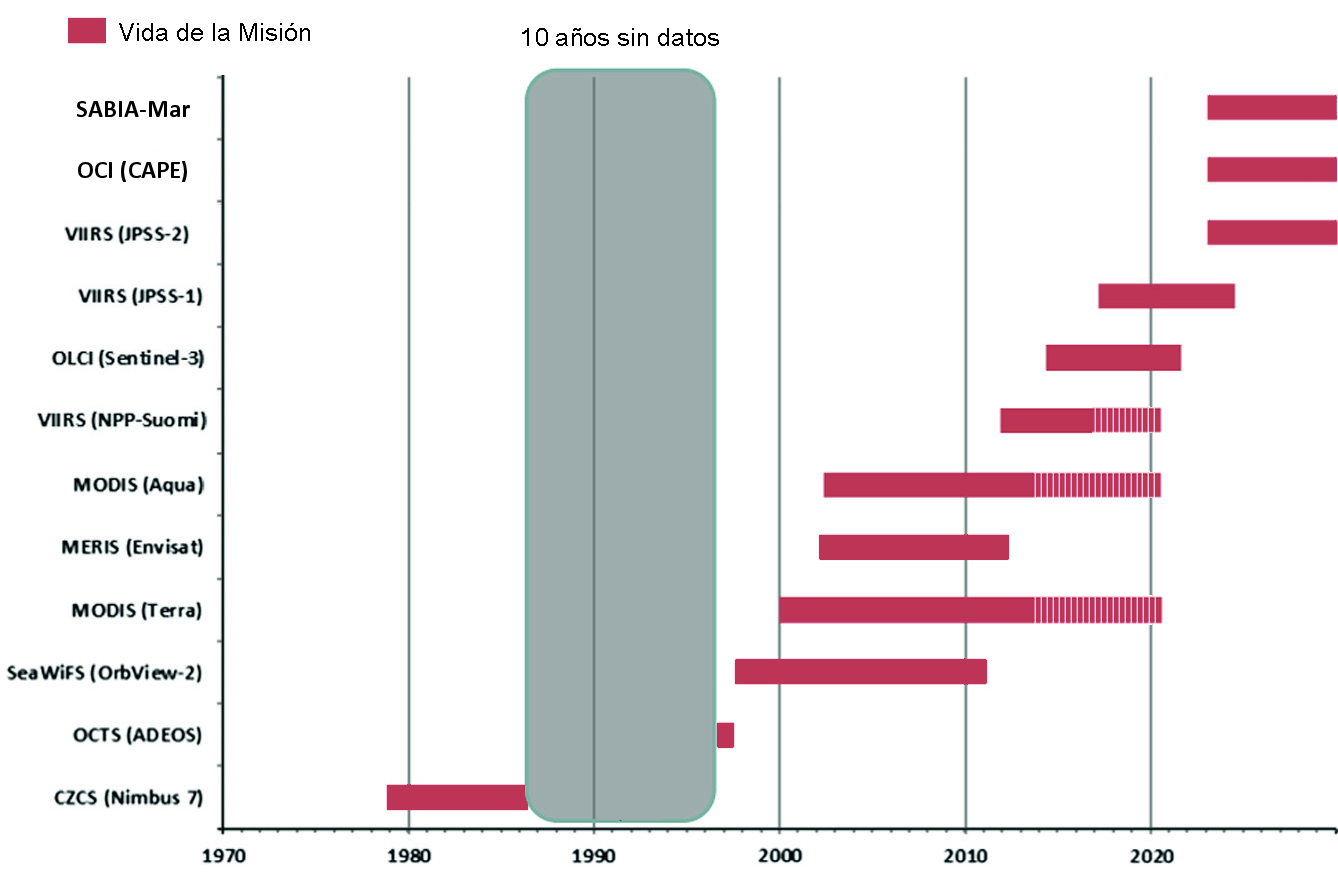
\includegraphics[width=\textwidth]{int/figures/sensor_timelines.png}
    \caption[Línea de tiempo con las principales misiones de color del mar en el período 1978-2030.]{Línea de tiempo con las principales misiones de color del mar en el período 1978-2030. Las barras indican el tiempo de vida útil y las barras rayadas verticalmente indican la extensión de la vida útil más allá del pronóstico inicial.}
    \label{int:sensor_timelines}
    \end{figure}

    \begin{table}
        \small
        \caption[Sensores utilizados en la presente tesis con sus características principales.]{Sensores utilizados en la presente tesis con sus características principales: ciclo de revisita, resolución espacial, rango espectral y número de bandas.}
        \begin{tabular}{|l|l|l|l|l|}
        \hline
        \textbf{Plataforma/Sensor}   & \textbf{\begin{tabular}[c]{@{}l@{}}Ciclo de revisita\\ {[}días{]}\end{tabular}} & \textbf{\begin{tabular}[c]{@{}l@{}}Resolución\\ espacial {[}m{]}\end{tabular}} & \textbf{\begin{tabular}[c]{@{}l@{}}Rango\\ espectral\\ {[}nm{]}\end{tabular}} & \textbf{\begin{tabular}[c]{@{}l@{}}Número\\ de bandas\end{tabular}} \\ \hline
        \textbf{Aqua-Terra/MODIS}    & 1    & 250/1000 & 400-2130 & 16 \\ \hline
        \textbf{LandSat-8/OLI}       & 16   & 30       & 433-2300 & 7  \\ \hline
        \textbf{SABIA-MAR/VNIR-SWIR} & 2    & 200      & 412-1640 & 16 \\ \hline
        \textbf{Sentinel-2/MSI}      & 5    & 10       & 443-2190 & 13 \\ \hline
        \textbf{Sentinel-3/OLCI}     & 2    & 300      & 400-1040 & 21 \\ \hline
        \textbf{Suomi-NPP/VIIRS}     & 1    & 750      & 410-2257 & 10 \\ \hline
        \end{tabular}
        \label{int:tab:sensores}
    \end{table}

    La ciencia del color del mar, posible gracias a la operatividad de estos sensores y a la comunidad científica que la desarrolla, ha demostrado su capacidad de proveer información sinóptica de las propiedades ópticas y biogeoquímicas de los océanos, \cite{tilstone2003b}\cite{blondeau2014}\cite{odermatt2016}. Esta se basa en la determinación de la radiancia espectral que proviene de la superficie del agua y ha demostrado ser una técnica muy fructífera ya que permite estimar la concentración de variables biogeofísicas como la concentración de clorofila-a, de material particulado en suspensión (\textit{Suspended Particulate Matter}, SPM) y la turbidez en áreas muy extensas y de manera periódica, resultando así una herramienta complementaria a las costosas mediciones de campo. Los datos satelitales del color del mar son utilizados para estudiar global y regionalmente la biosfera oceánica, su cambio en el tiempo y cómo se relaciona este cambio con las actividades antropogénicas. Los sensores satelitales de color del mar permiten detectar y cuantificar tendencias globales en las propiedades biogeoquímicas, tanto estacionales como en escalas temporales de décadas. Asimismo, constituyen una herramienta fundamental para la estimación de la producción primaria del \textit{fitoplancton} (organismos acuáticos autótrofos que tienen capacidad fotosintética y que viven dispersos en el agua) y que permite, junto con otras variables, delimitar zonas marinas de protección; como así también identificar potenciales zonas de pesca contribuyendo a un manejo sustentable de los recursos pesqueros, \cite{ioccg2008}.
    
    Las series temporales de propiedades de color del mar tienen aplicación en el estudio del cambio climático global \cite{dutkiewicz2019} - de hecho el color del mar ha sido clasificado como Variable Climática Esencial por el programa GCOS (\textit{Global Climate Observing System}) de la Organización Meteorológica Mundial (\textit{World Meteorological Organization}, WMO, \cite{wmoweb}). Mediante el conocimiento sobre la intensidad luminosa y la eficiencia fotosintética - obtenida mediante color del mar - es posible producir mapas de Producción Primaria Neta (Net Primary Production, NPP) sobre los océanos, es decir, indicadores de cuánto dióxido de carbono son capaces de fijar los organismos autótrofos y mixótrofos presentes en el agua, \cite{carr2006}. De esta forma, los datos del color del mar resultan esenciales en la determinación del balance global de dióxido de carbono, permitiendo mejorar el entendimiento de la tasa neta - actualmente positiva - de inyección de este gas de efecto invernadero en la atmósfera y los océanos.
    
    A su vez, los datos de color del mar junto con datos meteorológicos y de campo han sido utilizados para la detección temprana de floraciones algales nocivas, \cite{stumpf2003b}, a veces popularmente conocidas como \textit{mareas rojas}, las cuales impactan fuertemente en las actividades pesqueras. También han sido empleados para la detección y el análisis de la distribución espacial y temporal de zonas de máxima turbidez en diferentes ríos como el Río Girondo en Francia, \cite{doxaran2006}, o el Río de la Plata \cite{framinan1996}. En este último caso, la zona de máxima turbidez es un área de importancia económica y ecológica ya que es una zona de alta concentración de \textit{plancton} \cite{acha2004} y es el área principal de desove y de cría para muchas especies del estuario que se explotan comercialmente y sostienen las pesquerías costeras de Argentina y Uruguay, \cite{macchi1996}\cite{acha1999}\cite{jaureguizar2003}.
    
% ;  La complejidad adicional que supone la corrección atmosférica en aguas ópticamente complejas dio lugar a una variedad de alternativas, muchas de las cuales resultaron originalmente adecuadas en entornos de aguas moderadamente complejas \cite{stumpf2003}\cite{bailey2010}\cite{ruddick2000}, pero no en aguas extremadamente complejas como el Estuario del Río de la Plata - es decir, nuestra región de interés.
 
    Uno de los problemas más importantes a los que se enfrentan los científicos a la hora de dar uso a las imágenes obtenidas por los sensores de color del mar es la no transparencia de la atmósfera en las longitudes de onda de interés, por lo que es necesario el diseño de un algoritmo que remueva el efecto producido por la atmósfera en el flujo radiativo que, tras atravesar la atmósfera e interactuar con el entorno terrestre, arriba al sensor. Dicha metodología se denomina \textit{corrección atmosférica} (CA) y la primera en ser aplicada operativamente a imágenes ópticas fue diseñada por Howard Gordon para el pionero sensor CZCS, \cite{gordon1978}\cite{gordon1980}\cite{viollier1980}\cite{gordon1981}\cite{gordon1987}\cite{gordon1988}. Paradójicamente, el principio de funcionamiento de la CA radicaba en supuestos que se cumplían únicamente en aguas oligotróficas del océano abierto, siendo que el objetivo original de la puesta en órbita del CZCS era el monitoreo de aguas costeras, tal como su sigla lo indica. La no validez de dicho supuesto en aguas turbias se traducía en una mala estimación de las reflectancias del agua y, consecuentemente, en bajas concentraciones de clorofila-a, \cite{chavez1995}, un pigmento fotoactivo presente en la totalidad de los organismos fotosintéticos.

    Lo expuesto resalta que la precisión de las correcciones atmosféricas es fundamental en el área de color del mar dado que de ellas depende la capacidad de obtener la reflectancia medida justo sobre la superficie del agua, $\rho_{w}$, magnitud de base para los algoritmos bio-ópticos que la utilizan como entrada para estimar la concentración de diferentes propiedades ópticas o sustancias de interés. En general, del total de la radiación que llega al sensor, sólo una pequeña proporción de la misma corresponde a la señal que proviene del agua. Esta puede ser menor al 10\% en la región azul del espectro y mucho menor en las bandas infrarrojas, \cite{gordon1999}. Por lo tanto la aplicación de una corrección atmosférica sumamente precisa es fundamental para poder estimar plausiblemente el tipo y cantidad de sustancias presentes en el agua.
    
    La corrección diseñada e implementada por Howard Gordon para CZCS suponía que el agua absorbe toda la luz en la región del rojo e infrarrojo cercano (Near Infra-Red, NIR) del espectro electromagnético (supuesto de \textit{agua negra} o \textit{píxel negro}) permitiendo estimar la contribución de la atmósfera en esta región del espectro, extrapolarla a la región del visible ($400-600$ nm) y determinar así la componente que proviene de la capa superficial del agua y que contiene la información deseada (\S \ref{int:s:ACblackPixelNIR}). Sin embargo, en aguas altamente productivas o turbias, la alta concentración de partículas en suspensión incrementa mucho la dispersión de la energía en el NIR, por lo que la reflectancia del agua en esta región del espectro deja de ser nula - es decir que el supuesto de agua negra deja de ser válido, \cite{siegel2000}\cite{stumpf2003}. Asumir que la reflectancia del agua en el NIR es cero en aguas productivas o turbias lleva a una sobreestimación de la contribución de los aerosoles y subsecuentemente a una subestimación de la reflectancia del agua en la región visible del espectro, \cite{bailey2010}. Varios algoritmos han sido desarrollados con hipótesis alternativas o incluyendo esquemas que tienen en cuenta la contribución del agua en la señal total que llega al sensor \cite{stumpf2003}\cite{bailey2010}\cite{moore2011}\cite{ruddick2000}\cite{ruddick2006}, \S \ref{int:s:ACiterNIR},\ref{int:s:ACmumm}. Estos últimos algoritmos estiman o modelan la señal que proviene del agua en el NIR (supuesto de \textit{píxel brillante}) para luego restársela a la señal total y así poder aplicar la CA tradicional, es decir, utilizando el supuesto de agua negra. Otra estrategia propuesta ha sido utilizar bandas en longitudes de onda más largas en el infrarrojo de onda corta (Short Wave Infrared, SWIR, $1000-3000$ nm), donde la absorción del agua es tan alta que puede asumirse que la componente que proviene del agua sí es despreciable en esta región del espectro, \S \ref{int:s:ACswir}. Esto es equivalente a decir que dicha estrategia se respalda en el supuesto de agua negra, pero en el SWIR en vez del NIR. La problemática fundamental de dicha estrategia es que muchos de los sensores de color del mar carecen de dichas bandas o bien las poseen pero sin la suficiente relación señal ruido (\textit{Signal-to-Noise Ratio}, SNR), \cite{wang2018}.

    El color del mar es una variable fundamental para todas aquellas naciones con extensas líneas de costa con interés en monitorear y explotar su litoral marítimo, como es el caso de la República Argentina, donde recientemente nació la Iniciativa Pampa Azul \cite{pampaazul}, cuyo objetivo estriba en la imperante necesidad del país de continuar desarrollando una explotación eficiente y sustentable de sus recursos pesqueros. En el marco de la iniciativa, una de las regiones reconocidas de interés es el sistema fluvio-marino del Río de la Plata, cuyas aguas son críticas para las pesquerías costeras de especies como lenguado, pescadilla, gatuzo, raya, pez palo, corvina negra, saraca, pescadilla real y besugo, \cite{pampaazulrdp}. Por otro lado, la Comisión Nacional de Actividades Espaciales (CONAE) en conjunto con la Agencia Espacial Brasileña (AEB) y el Instituto Nacional de Investigación Espacial de Brasil (INPE) se encuentran actualmente desarrollando la misión SABIA-Mar, \cite{conaeSMar}\cite{invap}, cuyo principal objetivo es proveer información y productos para el estudio de los ecosistemas marinos, el ciclo del carbono, la cartografía de costas y hábitats marinos, peligros en el litoral marino, aguas continentales y las actividades pesqueras, \cite{conaeSMar}. Los sensores ópticos del SABIA-Mar tendrán bandas espectrales compatibles con los sensores SeaWiFS, MODIS, VIIRS, MERIS y OLCI. A su vez, SABIA-Mar contará con una resolución de 200 m en las áreas de interés específico que constituyen las zonas costeras y marítimas de Argentina y Brasil, como así también las aguas continentales de América del Sur, y una resolución de 800 m para estudios regionales y de cobertura global del océano con el fin de mantener una continuidad y compatibilidad con las demás misiones de color. Según se encuentra actualmente planeada la misión, SABIA-Mar contará con las bandas que también posee MODIS para la CA (tanto en el NIR como en el SWIR, a excepción de la banda en 2130 nm) más dos bandas que también han sido incorporadas en el sensor OLCI de la ESA, entre las cuales la banda en 1016 nm (SWIR cercano) ha demostrado ser útil tanto para la corrección atmosférica como para la estimación del SPM en aguas turbias, \cite{gossn2019}\cite{knaeps2012}.

    En este contexto, esta tesis fue concebida con el objetivo general de generar algoritmos alternativos de corrección atmosférica para ser aplicables sobre imágenes de sensores remotos con diferentes características espectrales en las aguas ópticamente complejas del Estuario del Río de la Plata, así como trabajar sobre aplicaciones novedosas del sensoramiento remoto en el visible sobre aguas con características ópticas afines. De esta forma, y en el marco de la Iniciativa Pampa Azul, esta tesis pretende generar un humilde aporte mediante el desarrollo de herramientas que permitan mejorar la comprensión del sistema fluvio-marino del Río de la Plata, de vital importancia económica para los países que lo conforman.
    
    En este capítulo presentaremos los antecedentes y los conceptos teóricos necesarios para un adecuado entendimiento de los capítulos posteriores. Partiremos definiendo brevemente las magnitudes físicas básicas utilizadas en el sensoramiento óptico de color del mar, partiendo del flujo radiante y concluyendo en la reflectancia del agua. Luego, describiremos las diferentes componentes del balance radiativo total que arriba al sensor, para después describir los diferentes procesos que son considerados por las CAs, necesarias para obtener la reflectancia del agua. Haremos particular hincapié en las diferentes estrategias existentes para la correcciones de aerosoles - la etapa más compleja de una CA - donde expondremos tanto el algoritmo estándar de corrección en aguas claras como las múltiples alternativas que surgen para corregir imágnes sobre escenarios de aguas ópticamente complejas. Describiremos a continuación nuestra área de estudio, el Estuario del Río de la Plata. Finalmente, presentaremos los objetivos de la tesis y un breve resumen del contenido de los capítulos posteriores.

\section{Magnitudes radiométricas utilizadas en teledetección}
\label{int:s:radiometricas}

    El sensoramiento remoto o la \textit{teledetección} es una técnica que permite adquirir información mediante el análisis de datos colectados por instrumentos que no están en contacto físico con los objetos investigados. Los sensores remotos, generalmente a bordo de aviones o satélites que orbitan la Tierra, miden la energía o radiación electromagnética (REM) que es reflejada o emitida por los objetos. Dicha radiación es cuantificada a partir de varias magnitudes físicas, entre las cuales están la irradiancia, la radiancia y la reflectancia, definidas a continuación. Se asumirán escenarios con campos de radiación estacionarios, por lo que se omitirá la dependencia del tiempo de las magnitudes presentadas.

	\subsection{Ángulos de observación-iluminación}
	\label{int:s:geometricas}
	
        Previo a introducir las magnitudes radiométricas, es necesario definir la convención usual utilizada en teledetección para determinar las direcciones de incidencia solar y de observación. En la Figura \ref{int:obs_ilum} se esquematiza el sistema sol-sensor en conjunto con los ángulos asociados a la geometría de observación-iluminación.
        
        \begin{figure}
        \centering
        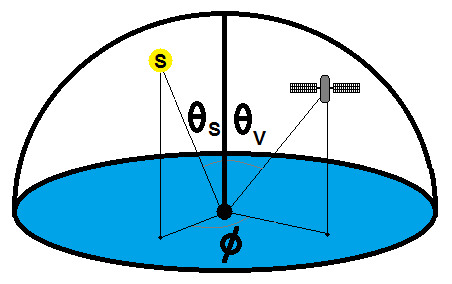
\includegraphics[width=0.5\textwidth]{int/figures/obs_ilum}
        \caption[Ángulos geométricos de observación-iluminación.]{Definición de los ángulos cenitales solar ($\theta_{s}$), de observación ($\theta_{v}$) y acimutal relativo sol-sensor ($\phi$), según la convención utilizada en esta tesis.}
        \label{int:obs_ilum}
        \end{figure}
    
        En general en teledetección se define la dirección en la cual se propaga la radiación en coordenadas esféricas, tomando como dirección polar el cenit; por lo que $\theta$ representa el ángulo cenital. El ángulo acimutal relativo $\phi$ se mide en sentido antihorario respecto del cenit desde el \textit{plano principal solar}, es decir, asumiendo un ángulo acimutal solar $\phi_{s}=0$. En el esquema de la Figura \ref{int:obs_ilum}, se determinan las dos direcciones más pertinentes: la del limbo solar y la de observación. En las definiciones dadas a continuación, donde aparezca la dupla $(\theta,\phi)$, esta referirá a una dirección de campo genérica, que podrá ser identificada con la dirección en que esté observando el sensor.

	\subsection{Irradiancia}
    \label{int:s:irradiancia}
        Considérese un flujo de energía radiativa atravesando un diferencial $dS$ de superficie plana. La tasa de flujo de energía radiativa, o potencia, por unidad de superficie se denomina \textit{irradiancia}, $E$, y es expresada en términos de energía neta $d^{2}U$ que atraviesa la superficie $dS$ en el intervalo temporal $[t,t+dt]$, o bien la potencia neta $d\Phi$ o \textit{flujo radiante} que atraviesa la superficie $dS$ como

        \begin{equation}
         E=\frac{d^{2} U}{dS\,dt}=\frac{d\Phi}{dS}\quad [W \cdot m^{-2}]
        \label{int:eq:irradiancia}
        \end{equation}

        La cantidad $d\Phi$ es diferencial de primer orden, considerada \textit{positiva} si el flujo radiante egresa del hemisferio superior (ascendente, $u$, suponiendo que la superficie sea horizontal) y \textit{negativa} en caso contrario (descendente, $d$). Es conveniente separar el flujo radiante en dos aportes positivos según si es ascendente o descendente, $d\Phi_{u}$ y $d\Phi_{d}$, cada uno de los cuales aporta una cantidad positiva de energía. Las irradiancias ascendente y descendente se definen entonces como
        
        \begin{equation}
         E_{u}=\frac{d\Phi_{u}}{dS}, \quad
         E_{d}=\frac{d\Phi_{d}}{dS}\quad [W\cdot m^{-2}]
        \label{int:eq:irrad_ascen_descen}
        \end{equation}
        
        El flujo radiante neto en la dirección ascendente es $d\Phi=d\Phi_{u}-d\Phi_{d}$. De la misma manera, la irradiancia neta es escrita como la diferencia entre dos cantidades positivas: $E=E_{u}-E_{d}$, siendo estas las medidas de toda la REM que sale y llega a una superficie, respectivamente (Figura \ref{int:irradiancia}).
        
        \begin{figure}
        \centering
        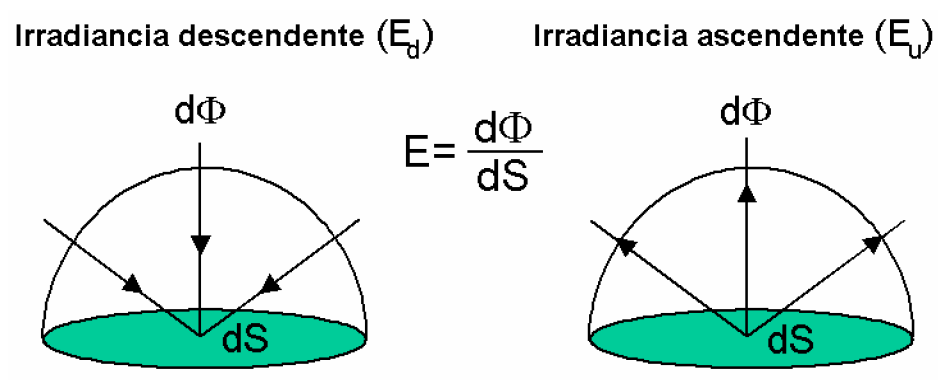
\includegraphics[width=0.6\textwidth]{int/figures/irradiancia}
        \caption[Esquematización de las irradiancias descendente ($E_{d}$) y ascendente ($E_{u}$).]{Esquematización de las irradiancias descendente ($E_{d}$) y ascendente ($E_{u}$), donde $d\Phi$ es el flujo radiante que llega a la superficie $dS$.} 
        \label{int:irradiancia}
        \end{figure}

	\subsection{Radiancia}
	\label{int:s:radiancia}
        Los sensores remotos tienen un campo limitado de observación y no detectan toda la irradiancia emitida por una superficie debido a que la forma del detector y su geometría de observación limitan la señal a una pequeña fracción del flujo. Esto implica que la dependencia del flujo radiante en función de la dirección tendrá un impacto sobre la energía detectada.
        %
        Teniendo en cuenta esto, consideremos un flujo radiante $d^{2}\Phi$ dentro de un ángulo sólido $d\Omega$ alrededor de la dirección $\hat{\Omega}$, atravesando un diferencial de superficie plana $dS$ (por ej. la superficie de un colector \textit{plano}) cuya orientación queda determinada por su normal $\hat{z}$ (ver Figura \ref{int:radiancia}). El ángulo comprendido entre $\hat{z}$ y la dirección de propagación $\hat{\Omega}$ es $\theta$. La potencia por unidad de superficie y por unidad de ángulo sólido se denomina \textit{radiancia}, $L(\theta,\phi)$, y viene dada por:
        
        \begin{equation}
         L(\theta,\phi)=\frac{d^{2}\Phi}{cos(\theta)dS\,d\Omega}\quad [W\cdot m^{-2} \cdot sr^{-1}]
        \label{int:eq:radiancia}
        \end{equation}

        \begin{figure}
        \centering
        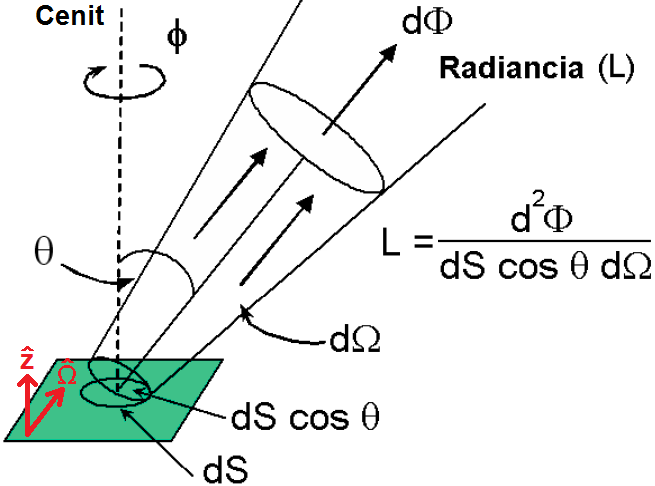
\includegraphics[width=0.6\textwidth]{int/figures/radiancia}
        \caption[Esquematización de la radiancia, $L(\theta,\phi)$, saliente de una superficie.]{Esquematización de la radiancia, $L(\theta,\phi)$, saliente de una superficie. Aquí, $dS$ representa el área de un elemento de la superficie, $L(\theta,\phi)$ es la radiancia que sale de $dS$ con un ángulo cenital $\theta$ (relativo a la normal $\hat{z}$) y un ángulo acimutal $\phi$. Su valor es definido por el flujo radiante que sale de $dS$ dentro del ángulo sólido $d\Omega$, centrado en la línea definida por $\theta$ y $\phi$.} 
        \label{int:radiancia}
        \end{figure}

        Nótese que, además de haber dividido por $d\Omega dS$, se ha dividido por el factor $cos(\theta) = \hat{z}\cdot \hat{\Omega}$, es decir, la proyección del elemento de superficie al plano normal a $\hat{\Omega}$. Es por esto que un colector de radiación plano se denomina \textit{colector coseno}. Nótese también que si $\hat{z}$ y $\hat{\Omega}$ apuntan en hemisferios opuestos, entonces $\hat{z}\cdot \hat{\Omega}$ es negativo. El flujo radiante es también negativo en este caso, por definición; por lo que la relación $d^{2}\Phi/cos(\theta)$ se mantiene positiva: la radiancia es siempre positiva.             Se obtendrá la relación entre radiancia e irradiancia a partir de la Ec. \ref{int:eq:radiancia}, que se podrá reescribir como

        \begin{equation}
         d^{2}\Phi=L(\theta,\phi)cos(\theta) dS d\Omega
        \label{int:eq:radiancia_dif}
         \end{equation}
        
        Utilizando las Ecs. \ref{int:eq:irradiancia} y \ref{int:eq:radiancia_dif} se obtienen las siguientes relaciones entre irradiancias (ascendente y descendente) y radiancia:

        \begin{equation}
        E_{u}=\left|\frac{d\Phi_{u}}{dS}\right|=\int_{+}d\Omega L(\theta,\phi)cos(\theta),\quad  E_{d}=\left|\frac{d\Phi_{d}}{dS}\right|= - \int_{-}d\Omega L(\theta,\phi)cos(\theta)
        \label{int:eq:rad_irrad1}
        \end{equation}
        
        \noindent donde + y - indican que se integra sobre los hemisferios superior e inferior, respectivamente. Sendas magnitudes son definidas positivas. Combinándolas, se obtiene que \textit{la irradiancia neta es la integración de la radiancia sobre todo el ángulo sólido},
        
        \begin{equation}
         E=E_{u} + E_{d}=\int_{4\pi}d\Omega L(\theta,\phi)|cos(\theta)|\quad [W\cdot m^{-2}]
        \label{int:eq:rad_irrad2}
         \end{equation}
        

        % \begin{enumerate}
        % \item \textbf{Radiancia proveniente del limbo solar}. En caso de despreciar el ángulo sólido abarcado por el limbo solar en el cielo terrestre, la radiancia solar incidente, previa a interactuar con la atmósfera, puede ser escrita como
        
        % \begin{equation}
        % L_{s}(\theta,\phi)(\hat{\Omega})=E_{s}\delta(\hat{\Omega}-\hat{\Omega}_{s})
        % \label{limbosolar}
        %  \end{equation}
        
        % \noindetsiendo siendo $\hat{\Omega}_{s}=(\theta_{s}, \phi_{s}=0)$ la dirección en la que se halla el limbo solar, $\delta(\hat{\Omega}-\hat{\Omega}_{s})=\delta(\phi)\delta(cos \theta - cos \theta_{s})$ la distribución delta de Dirac bidimensional, y $E_{s}$ la irradiancia solar extraatmosférica.
        
        A continuación, describiremos dos casos límite en la distribución angular de la radiancia: 

        \subsubsection{Radiancia saliente de una superficie lambertiana}
        \label{int:s:lambertiana}
        
            En caso de incidir sobre una superficie horizontal que sea un difusor perfecto, o sea una superficie que emite o refleja la energía con la misma intensidad en todas las direcciones independientemente del ángulo con el que incide la radiación, tendríamos, en las cercanías de la misma, siguiendo la Ec. \ref{int:eq:rad_irrad1},
            
            \begin{equation}
            E_{u}=E_{d}=\pi L
            \label{int:eq:lambertiana}
            \end{equation}
            
            A este tipo de superficies se las llama \textit{lambertianas} (Figura \ref{int:lambertiana}a).
            Ninguna superficie es perfectamente lambertiana, pero muchas de ellas, especialmente las opacas, se aproximan bastante (como la placa Spectralon utilizada en algunas mediciones radiómetricas de campo, ver \S \ref{dat:s:asdMed}).
        
        \subsubsection{Radiancia saliente de una superficie especular}
        \label{int:s:especular}
        
            Como caso opuesto a una superficie lambertiana puede mencionarse la superficie especular (Figura \ref{int:lambertiana}b). En este tipo de superficie la energía es reflejada con un ángulo igual al incidente pero en sentido opuesto, por lo que podremos afirmar que
            
            \begin{equation}
            L_{u}(\theta,\phi, z = 0^{+}) \propto L_{d}(\theta,-\phi, z = 0^{+})
            \label{int:eq:especular}
            \end{equation}
            
            \noindent donde hemos asumido una superficie planar horizontal. Una superficie natural que se aproxima bastante a este límite es la interfase agua-aire de una laguna profunda de aguas claras un día sin viento y vista en el rango NIR - donde valdría el supuesto de agua negra. En tal caso, la interfase se comportaría como un espejo que reflejaría siguiendo las leyes de Fresnel. Las superficies naturales en general se comportan de forma intermedia entre los casos lambertiano y especular (Figura \ref{int:lambertiana}c).
            
            \begin{figure}
            \centering
            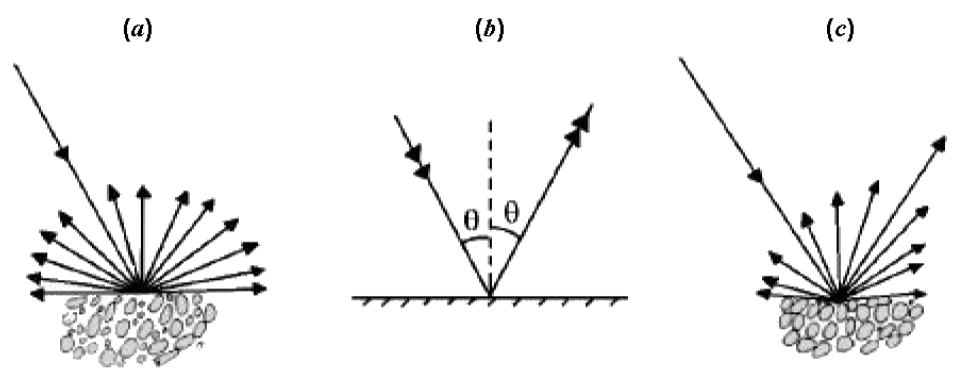
\includegraphics[width=0.75\textwidth]{int/figures/lambertiana}
            \caption[Diferentes tipos de superficies reflectoras: difusa, especular y mixta.]{Diferentes tipos de superficies reflectoras: (a) difusa o lambertiana, (b) especular y (c) tipo mixta.} 
            \label{int:lambertiana}
            \end{figure}
            % \end{enumerate}
        
	\subsection{Reflectancia y color del mar}
	\label{int:s:reflectancia}

        Todas las propiedades ópticas del agua varían con la longitud de onda ($\lambda$), por lo tanto se definen la irradiancia espectral, $E(\lambda)$, y la radiancia espectral, $L(\lambda,\theta,\phi)$, de manera análoga pero considerando radiación en el rango espectral diferencial $[\lambda,\lambda+d\lambda]$, es decir:

        \begin{align}
         &E(\lambda)=\frac{d E}{d\lambda}(\lambda) \quad [W m^{-2} nm^{-1}] \\
         &L(\lambda,\theta,\phi)=\frac{d L}{d\lambda}(\lambda,\theta,\phi) \quad [W m^{-2} sr^{-1} nm^{-1}]
        \label{int:eq:depEspectral}
        \end{align}
        
        La magnitud radiométrica de base del color del mar está determinada por la variación espectral de la reflectancia superficial irradiante o \textit{reflectancia del agua}, $\rho_{w}(\lambda)$, definida como el cociente entre la irradiancia ascendente, $E_{u}$, y la irradiancia descendente, $E_{d}$, justo por encima del agua ($z=0^{+}$), o sea:
        
        \begin{equation}
        \rho_{w}(\lambda)=\frac{E_{u}(\lambda,z=0^{+})}{E_{d}(\lambda,z=0^{+})} \quad [s/u]
        \label{int:eq:reflectancia}
        \end{equation}
        
        Dicha normalización por la irradiancia descendente le confiere a la reflectancia del agua la cualidad de propiedad óptica (cuasi) inherente (\textit{Inherent Optical Property}, IOP), es decir, (casi) independiente de las condiciones específicas del campo de iluminación (ángulo de incidencia del sol, estado de la atmósfera, etc.). Es por esto que la reflectancia es la magnitud radiométrica de la que se parte para la estimación de las diferentes sustancias presentes en el agua; aunque en realidad los sensores remotos no miden la irradiancia ascendente completa - presente en la Ec. \ref{int:eq:reflectancia} -; sino una porción de la misma. Por esto, muchas veces se prefiere expresar el color intrínseco del mar en función de la reflectancia sensada remótamente, $R_{rs}$:
        
        \begin{equation}
        R_{rs}(\theta,\phi,\lambda)=\frac{L_{u}(\theta,\phi,\lambda,z=0^{+})}{E_{d}(\lambda,z=0^{+})} \quad [sr^{-1}]
        \label{int:eq:rrs}
        \end{equation}
        
        \noindent pudiéndose establecer, en caso de asumir la superficie del agua como lambertiana (Ec. \ref{int:eq:lambertiana}), que

        \begin{equation}
        \rho_{w}(\lambda)=\pi R_{rs}(\lambda)
        \label{int:eq:rrsVsRho}
        \end{equation}

\section{El problema de la corrección atmosférica}
\label{int:s:componentes}
    
    Para poder esbozar más detalladamente cuál es el objetivo de aplicar una CA sobre imágenes de color es necesario conocer cuáles son las componentes que afectan la señal que arriba al sensor. La radiancia \textit{que arriba al sensor a TOA} (\textit{Top Of Atmosphere} en inglés) tras haber interactuado con el sistema óptico atmósfera-océano puede modelarse como la suma de diferentes términos que provienen de cada una de las diferentes componentes físicas del sistema. Una posible forma de descomponerla es:
    
    \begin{equation}
        L_{TOA} = L_{R} + [L_{A}+L_{RA}] + L_{g,TOA} + L_{sky,TOA} + L_{wc,TOA} + L_{w,TOA}
        \label{int:eq:ltoa}
    \end{equation}

    \noindent donde cada uno de los términos del lado derecho corresponden a radiancias conformadas por flujos de fotones que interactúan con las siguientes componentes:
    
    \begin{enumerate}
        \item $L_{R}$: fotones que fueron dispersados por moléculas de aire (y no arribaron a superficie).
        \item $L_{A}$: fotones que fueron dispersados por aerosoles (y no arribaron a superficie).
        \item $L_{RA}$: fotones que fueron dispersados por aerosoles y moléculas (dispersión indefectiblemente múltiple).
        \item $L_{g,TOA}$: fotones reflejados especularmente por la interfase del agua, provenientes directamente del limbo solar (\textit{sunglint}).
        \item $L_{sky,TOA}$: fotones reflejados especularmente por la interfase del agua, provenientes del campo de iluminación difusa del cielo (\textit{skyglint}).
        \item $L_{wc,TOA}$: fotones provenientes de la espuma que se halla en la superficie (\textit{whitecaps}).
        \item $L_{wc,TOA}$: fotones que fueron retrodispersados y reemergen del interior del cuerpo de agua.
    \end{enumerate}

    Es fundamental notar aquí que la radiancia es una Propiedad Óptica Aparente (\textit{Apparent Optical Property}, AOP), es decir, depende fuertemente del campo de iluminación. Para poder llegar a una expresión que contenga reflectancias (cuasi-IOPs), es necesario normalizar la expresión de la Ec. \ref{int:eq:ltoa} por la radiancia solar descendente a TOA, que no se mide si no que se calcula según:

    \begin{equation}
        E_{d,TOA} = F_{0}\left(\frac{R_{0}}{R}\right)^{2}cos(\theta_{s})
        \label{int:eq:edtoa}
    \end{equation}

    \noindent donde $F_{0}$ es la irradiancia solar extraatmosférica cuando el Sol se halla a $R_{0} = 1$ unidad astronómica de la Tierra (Figura \ref{int:hiper_thuillier}); el factor $\left(\frac{R_{0}}{R}\right)^{2}$ es el factor de adecuación de la irradiancia solar a la distancia real Sol-Tierra que varía con el día del año, siendo $R$ la distancia Tierra-Sol (Ley del Cuadrado Inverso de la Distancia) y $cos(\theta_{s})$ es el factor de corrección por el apartamiento del Sol del cenit (Ley del Coseno de Lambert). Considerando esta expresión para la irradiancia descendente a TOA, se define la reflectancia a TOA, $\rho_{TOA}$ siguiendo la Ec. \ref{int:eq:reflectancia} como

    \begin{equation}
        \rho_{TOA} = \frac{E_{u,TOA}}{E_{d,TOA}}\approx \frac{\pi L_{TOA}}{F_{0}\left(\frac{R}{R_{0}}\right)^{2}cos(\theta_{s})}
        \label{int:eq:rhotoa0}
    \end{equation}

    \begin{figure}
    \centering
    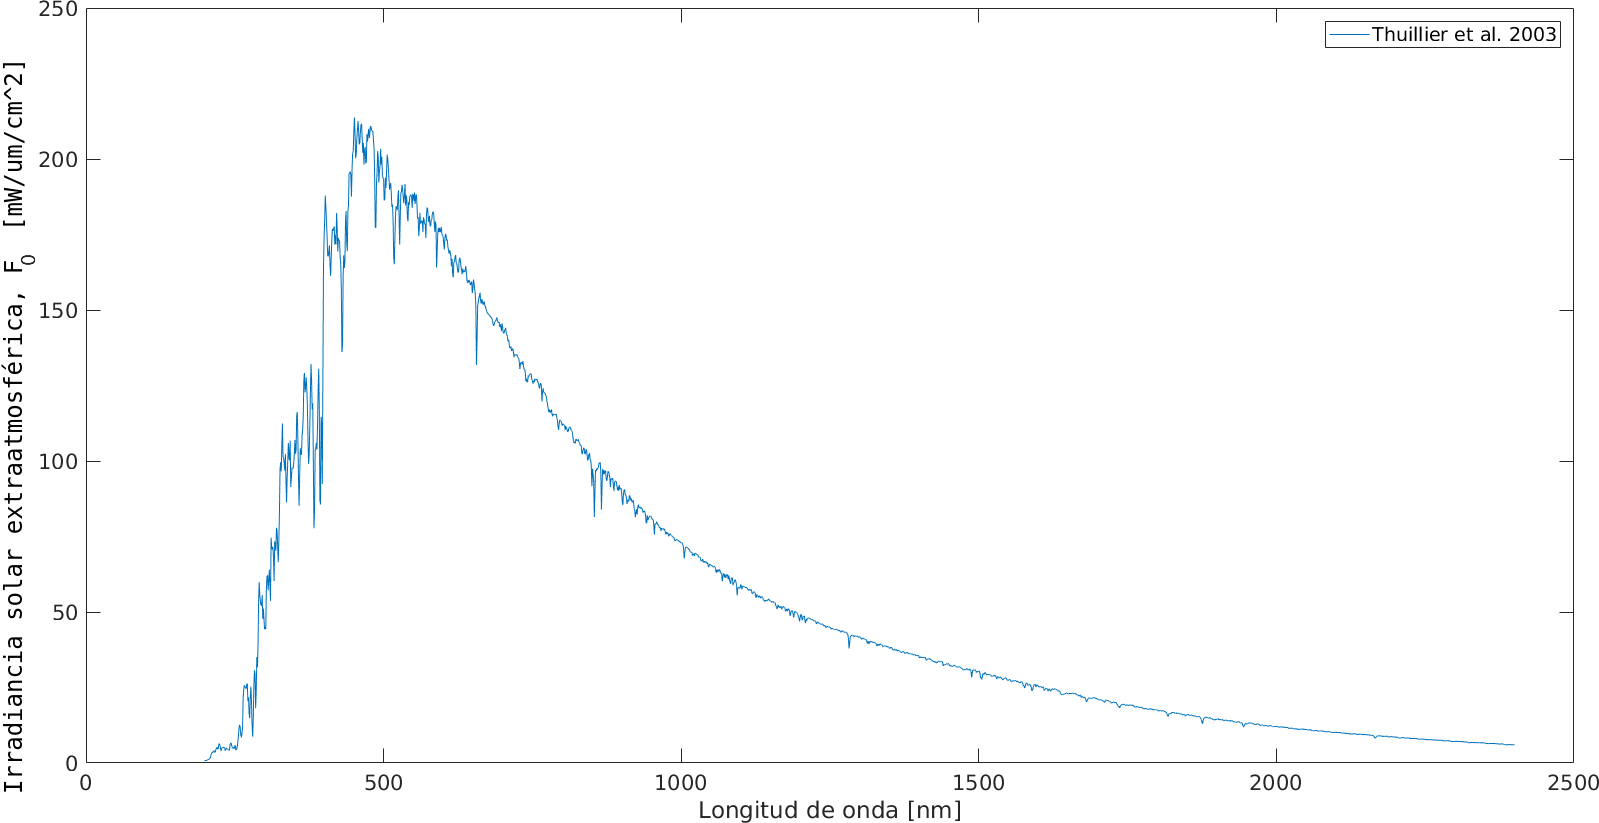
\includegraphics[width=\textwidth]{int/figures/hiper_thuillier.png}
    \caption[Irradiancia solar extraatmosférica (a $R = 1 UA$).]{Irradiancia solar extraatmosférica (a $R = 1 UA$) media medida por el espectrómetro SOLSPEC, Thuillier et al. 2003, \cite{thuillier2003}}
    \label{int:hiper_thuillier}
    \end{figure}

    \noindent donde el factor $\pi$ se utiliza como coeficiente de proporcionalidad entre la radiancia a TOA e irradiancia a TOA, es decir, se asume que la superfcie terrestre es  lambertiana (Ec. \ref{int:eq:lambertiana}). Si bien esta hipótesis no es válida, la expresión dada en Ec. \ref{int:eq:rhotoa0} se suele aplicar como convención y luego se aplica una corrección para minimizar el error introducido por esta hipótesis intentando reproducir la real Función de Distribución Bidireccional de la Reflectancia (\textit{Bidirectional Reflectance Distribution Function}, BRDF). Dicha corrección se suele aplicar directamente sobre la reflectancia del agua siguiendo el procedimiento culminado en Morel y Gentili 2002, \cite{morel2002}. Si embargo, en cuerpos de agua turbios como el RdP no se aplica debido a que dicha corrección fue diseñada para aguas ópticamente claras, y en caso de aplicarla introduciría mayor error en las estimaciones de reflectancias del agua (véase por ej. Li et al. 2019, \cite{li2019}). Una vez aplicado este factor, la expresión dada en la Ec. \ref{int:eq:ltoa} se puede expresar idénticamente, pero en reflectancias:

    \begin{equation}
        \rho_{TOA} = \rho_{R} + [\rho_{A} + \rho_{RA}] + \rho_{g,TOA} + \rho_{wc,TOA} + \rho_{w,TOA}
        \label{int:eq:rhotoa1}
    \end{equation}

    \noindent donde el término de \textit{skyglint} no figura pues fue incluido dentro del término $\rho_{R}$, dado que será corregido junto con la corrección por Rayleigh (véase \S \ref{int:s:rayleigh}). Es importante notar aquí que el sufijo \textit{TOA} que figura en los términos de superficie indica que dichas reflectancias no siguen exactamente la definición de reflectancia dada en la Ec. \ref{int:eq:reflectancia}, dado que no corresponden al cociente de irradiancias de salida y de entrada justo por encima de la superficie ($0^{+}$), sino al cociente a TOA. Para saber cómo relacionar estos términos con reflectancias de superficie reales es necesario establecer la relación entre las irradiancias a TOA y las irradiancias a $0^{+}$. Esto suele hacerse intoduciendo factores de \textit{transmitancia} que representan el efecto de la atmósfera sobre los términos de superficie. Por ejemplo, para el término de reflectancia del agua, se tiene que:

    \begin{equation}
        \rho_{w}(0^{+}) = \frac{E_{w}(0^{+})}{E_{d}(0^{+})} = \frac{\pi L_{w}(0^{+})}{E_{d,TOA}t_{s}t_{gs}} = \frac{\pi \frac{L_{w,TOA}}{t_{v}t_{gv}}}{E_{d,TOA}t_{s}t_{gs}} 
        \label{int:eq:rhowsupVStoa0}
    \end{equation}

    \noindent donde $E_{w}(0^{+})$ y $L_{w}(0^{+})$ son la radiancia y la irradiancia ascendente, medidas justo por encima de la superficie del agua; $t_{gs}$ y $t_{gv}$ son las transmitancias debidas a la absorción de moléculas de aire (véase \S \ref{int:s:tAbs}) en los caminos del Sol a la superficie y de la superficie al sensor, y $t_{s}$ y $t_{v}$ son las \textit{transmitancias difusas} (véase \S \ref{int:s:tDif}) - aplicables a radiancias lambertianas - debidas a fenómenos dispersivos en la atmófera. Obsérvese que nuevamente hemos asumido una relación entre la irradiancia y la radiancia asociada a la presencia de una superficie reflectora lambertiana. También es importante notar que las transmitancias son coeficientes que toman valores en el rango $[0-1]$, es decir que en general $t<1$ - pero cercana a 1 en ciertas regiones del espectro que se utilizan para el sensoramiento remoto usualmente llamadas \textit{ventanas atmosféricas} - por lo que, naturalmente $E_{d}(0+)<E_{d,TOA}$ y $L_{w}(0+)>L_{w,TOA}$. Es evidente que, reordenando la Ec. \ref{int:eq:rhowsupVStoa0}, obtenemos la siguiente relación:

    \begin{equation}
        \rho_{w}(0^{+}) = \frac{\rho_{w,TOA}}{t_{s}t_{v}t_{gs}t_{gv}}
        \label{int:eq:rhowsupVStoa}
    \end{equation}

    Debido a que el término de espuma (\textit{WC}) es aproximadamente lambertiano, \cite{gordon1994b}, la relación entre $\rho_{wc}(0^{+})$ y $\rho_{wc,TOA}$ es equivalente a la dada en Ec. \ref{int:eq:rhowsupVStoa0}. Por otro lado, el término debido al \textit{sunglint} corresponde al caso de una reflexión especular (Ec. \ref{int:eq:especular}), por lo que el factor que se aplica para representar el acople del \textit{sunglint} con la dispersión atmosférica es el de \textit{transmitancia directa}, $T$ (véase \S \ref{int:s:tDir}), resultando entonces

    \begin{equation}
        \rho_{g}(0^{+}) = \frac{\rho_{g,TOA}}{T_{ds}T_{dv}t_{gs}t_{gv}}
        \label{int:eq:rhogsupVStoa}
    \end{equation}
    
    La absorción de moléculas de aire también afectará a los términos atmosféricos puros y podremos desacoplarla - en los casos del ozono ($O_{3}$) y el dióxido de nitrógeno ($NO_{2}$) estratosféricos - de los efectos dispersivos (mayormente troposféricos, \S \ref{int:s:tAbs}), de forma tal que

    \begin{equation}
        \rho_{R} + [\rho_{A} + \rho_{RA}] = (\rho_{r} + [\rho_{a} + \rho_{ra}])t_{gs}t_{gv}
        \label{int:eq:rhorAbs}
    \end{equation}

    \noindent donde las reflectancias con subíndices minúsculos representan a los fenómenos dispersivos en ausencia de absorción de moléculas de aire. Tras haber considerado todos estos procesos, la descomposición de la reflectancia a TOA puede escribirse como

    \begin{equation}
        \rho_{TOA} = \underbrace{t_{g}}_\text{A}.(\underbrace{\rho_{r}}_\text{B} + \underbrace{[\rho_{a} + \rho_{ra}]}_\text{C} + \underbrace{T}_\text{D}.\underbrace{\rho_{g}}_\text{E} + \underbrace{t}_\text{F}.[\underbrace{\rho_{wc}}_\text{G} + \underbrace{\rho_{w}}_\text{H}])
        \label{int:eq:rhotoa}
    \end{equation}

    \noindent donde hemos expresado las transmitancias sol-superficie (\textit{s}) y superficie-sensor (\textit{v}) en transmitancias de dos caminos, por ej. $t = t_{s}t_{v}$. El objetivo de la corrección atmosférica radica en aislar el término $\rho_{w}$ (H) del resto de los términos, originados en la atmósfera y en la interfase aire-agua (A-G). A continuación, para cada uno de estos términos, haremos una breve caracterización de sus propiedades, así como de los esquemas estándares de estimación para su corrección aplicados a cada uno. Es importante destacar que en este análisis obviaremos otros pasos estándares de CA, todos detallados en el tutorial de Mobley et al. 2016, \cite{mobley2016}, y descritos muy brevemente a continuación:
    
    \begin{enumerate}
        \item \textbf{Calibración vicaria}. Típicamente, las reflectancias del agua obtenidas tras aplicar una CA sobre una imagen de color no son exactamente coincidentes con las reflectancias medidas por radiómetros de campo debido a inexactitudes en el proceso de corrección, degradación de diferentes componentes del sensor satelital o inexactitudes en las mediciones \textit{in situ}. Es por esto que típicamente se utilizan sitios de calibración específicos que cuentan con mediciones de campo - tanto de la reflectancia del agua como del estado de la atmósfera - que se asumen como verdaderas (\textit{ground-truth}) y, estableciendo el apartamiento entre las mediciones de campo y las estimaciones satelitales, se computan coeficientes globales que se aplican directamente a las reflectancias del agua estimadas por el satélite. Esto se hace con el objetivo de que las estimaciones satelitales resulten lo más coincidentes posible con las mediciones de campo. Esto define una Calibración Vicaria del Sistema (\textit{System Vicarious Calibration}, SVC) - llamados así porque son calculados con el sensor en órbita - y son un proceso usual aplicado sobre las reflectancias del agua satelitales. Genéricamente corresponderá un conjunto diferente de coeficientes de calibración vicaria para cada esquema diferente de CA aplicada y para cada sensor.
        \item \textbf{Corrección por sensibilidad fuera de banda (\textit{Out-Of-Band sensitivity}, OOB)}. Las Funciones de Respuesta Espectral, (\textit{Spectral Response Function}, SRF), muchas veces toman valores no nulos en longitudes de onda muy alejadas a la central. En tal caso se computan factores de corrección que relacionan las SRFs reales - es decir, con sensibilidad OOB - con SRFs razonables que no consideren longitudes de onda demasiado alejadas de la nominal. Se discute en \cite{mobley2016} cuándo es importante aplicar dicha corrección y cuándo no.
        \item \textbf{Corrección por sensibilidad a la polarización}. Se debe aplicar debido a diferencias - indeseadas - en las mediciones de ciertos radiómetros de color debidas a diferentes estados de polarización de la radiación incidente. Típicamente se computa un factor de corrección, \cite{mobley2016}, basado en i) una caracterización pre-lanzamiento de la matriz de Mueller del sensor - que describe la sensibilidad a las diferentes polarizaciones -, y ii) en simulaciones de transferencia radiativa que consideran únicamente las componentes de más impacto en el grado de polarización dentro del balance de la Ec. \ref{int:eq:rhotoa}: la dispersión Rayleigh molecular y el \textit{sunglint}.
    \end{enumerate}

\section{Absorción molecular (A)}
\label{int:s:tAbs}

    Algunas de las componentes naturales del aire son absorbentes. Existen dos tipos de componentes absorbentes: las mayormente troposféricas (vapor de agua, $H_{2}O$, y oxígeno, $O_{2}$) y las mayormente estratosféricas (ozono, $O_{3}$ y dióxido de nitrógeno, $NO_{2}$).
    
    Dado que los fenómenos de dispersión atmosférica ocurren mayormente en la troposfera, la absorción debida a los gases troposféricos (oxígeno y vapor de agua) es más complicada de corregir, puesto que está fuertemente acoplada a los procesos de dispersión. Esto implica que, dado un fotón en la troposfera, el camino óptico recorrido en la atmósfera es difícil de computar dado que pudo estar sometido a múltiples procesos de dispersión; por lo que es difícil encontrar una expresión para el factor de transmitancia. Afortunadamente, las líneas de absorción de dichas moléculas en el visible son bastante angostas y pueden ser evitadas definiendo bandas que no se vean afectadas por las mismas (Figura \ref{int:oxigeno_h20_Mobley}).

    \begin{figure}
    \centering
    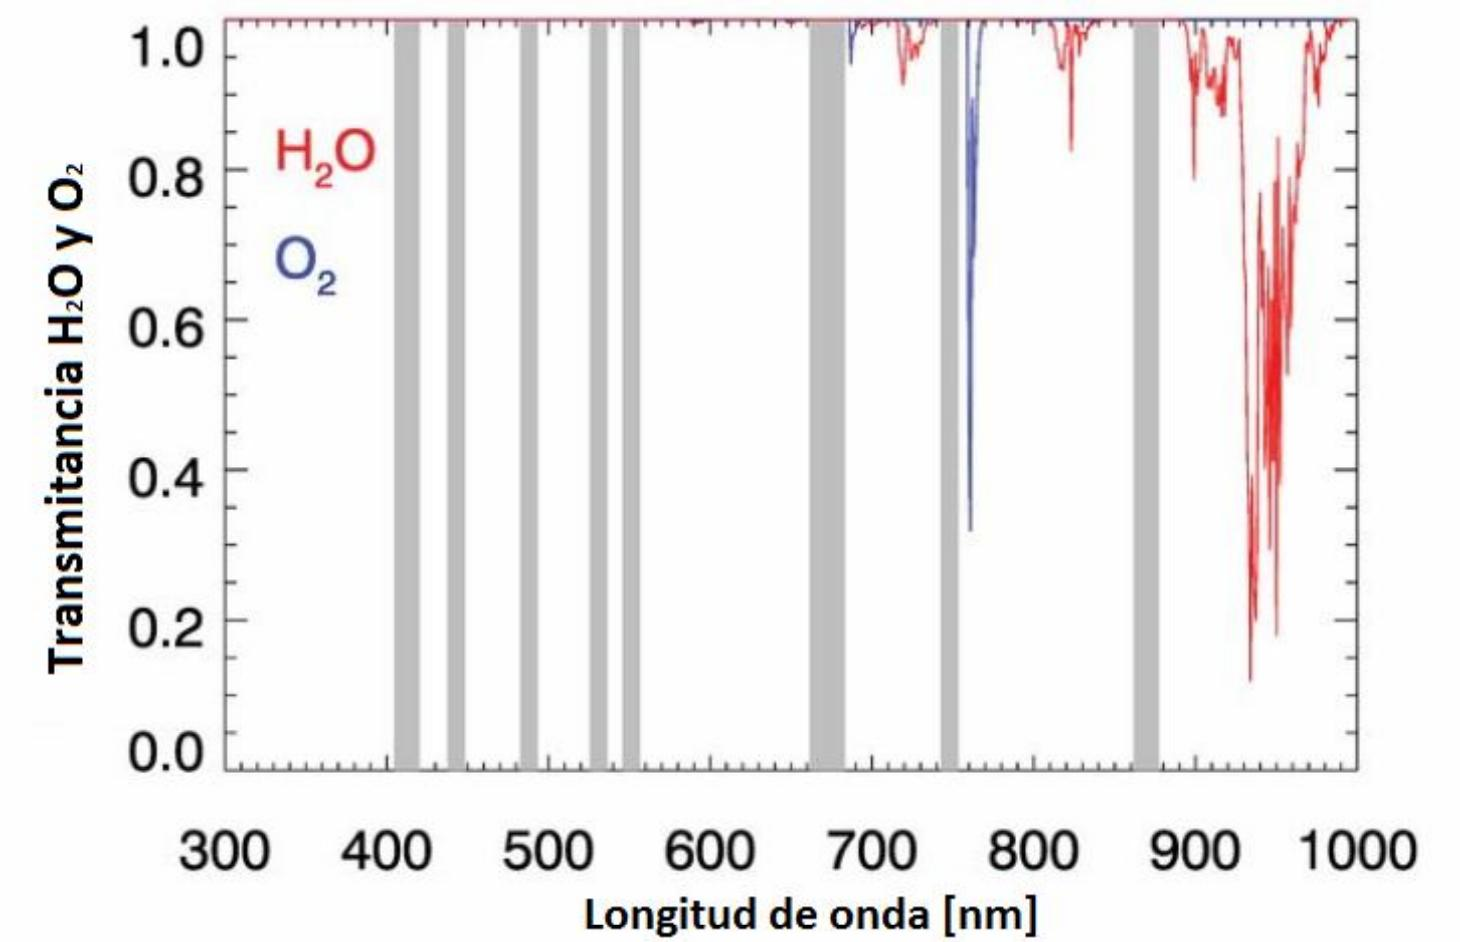
\includegraphics[width=0.7\textwidth]{int/figures/oxigeno_h20_Mobley.png}
    \caption[Transmitancias debidas a la absorción del oxígeno y del vapor de agua.]{Transmitancias debidas a la absorción del oxígeno, $O_{2}$, y del vapor de agua, $H_{2}O$ para una atmósfera húmeda tropical. La resolución es de 1 nm. Figura de Mobley et al. 2016, \cite{mobley2016}.}
    \label{int:oxigeno_h20_Mobley}
    \end{figure}

    Por el contrario, tanto el ozono como el dióxido de nitrógeno se hallan principalmente en la estratósfera, por lo que su acople con los procesos de dispersión es bajo y se podrá asumir la siguiente expresión:

    \begin{equation}
        t_{g}^{O_{3} + NO_{2}} = t_{g}^{O_{3}}(\lambda,[O_{3}],\mu) \times t_{g}^{NO_{2}}(\lambda,[NO_{2}],\mu)
        \label{int:eq:tAbsO3NO2}
    \end{equation}

    \noindent es decir, que el factor de transmitancia total dado por el efecto conjunto de $O_{3}$ y $NO_{2}$ podrá ser factoreado y estimado a partir de sus concentraciones, $[O_{3}]$ y $[NO_{2}]$, y el factor geométrico de masa de aire ($\mu$) dado por los ángulos cenitales de iluminación ($\theta_{s}$) y observación ($\theta_{v}$):
    
    \begin{equation}
        \mu = \frac{1}{cos(\theta_{s})} + \frac{1}{cos(\theta_{v})}
        \label{int:eq:mu}
    \end{equation}

    \noindent sin contemplar ningún efecto de acople con otros efectos atmosféricos, como la dispersión molecular o la presencia de aerosoles. A su vez, cada uno de estos factores puede expresarse a partir de sus respectivos coeficientes de extinción ($k$) según:

    \begin{equation}
        t_{g}^{O_{3} }(\lambda,[O_{3}],\mu) = e^{-k_{O_{3} }(\lambda)[O_{3} ]\mu}
        \label{int:eq:tAbsExpKCTCMU_O3}
    \end{equation}

    \begin{equation}
        t_{g}^{NO_{2}}(\lambda,[O_{3}],\mu) = e^{-k_{NO_{2}}(\lambda)[NO_{2}]\mu}
        \label{int:eq:tAbsExpKCTCMU_NO2}
    \end{equation}
    
    Los valores de $k_{O_{3}}$, expresado como el coeficiente de atenuación (en cm$^{-1}$) cada 1 nm entre 200 y 2550 nm, así como el $k_{NO_{2}}$, expresado como la sección eficaz de absorción del $NO_{2}$ (en cm$^{2}$/molécula) cada 1 nm entre 200 y 2540 nm, pueden ser obtenidos del sitio del \textit{Ocean Biology Processing Group} de la NASA \cite{obpg}. Es importante notar que las expresiones dadas en las Ecs. \ref{int:eq:tAbsExpKCTCMU_O3} y \ref{int:eq:tAbsExpKCTCMU_NO2} corresponden a transmitancias de dos sentidos (sol-superficie y superficie-sensor, tal como las que figuran en la Ec. \ref{int:eq:rhotoa}).
    
    Para computar los valores de los factores dados en la Ec. \ref{int:eq:tAbsO3NO2} es necesario conocer las concentraciones de ozono y dióxido de nitrógeno. Si bien estas pueden obtenerse a partir de datos de satelites meteorológicos (como el TOMS/EPTOMS - Total Ozone Mapping Spectrometer onboard the Earth Probe spacecraft - de la NASA), o de re-análisis (por ej. el provisto por el European Centre for Medium-Range Weather Forecasts, ECMWF), muchas veces no se dispone de dicha información, por lo que se deben asumir valores nominales de $[O_{3}]$ y $[NO_{2}]$. Los valores típicos son de:

    \begin{equation}
        [O_{3}] = 80.7\times10^{16} part/cm^{2} = 300 DU
        \label{int:eq:conc_o3}
    \end{equation}
    \begin{equation}
        [NO_{2}] = 1.1 \times10^{16} part/cm^{2}
        \label{int:eq:conc_no2}
    \end{equation}

    En la Figura \ref{int:O3_RDP_ECMWF} se puede observar la concentración de ozono provista por el re-análisis de ECMWF (cuyos mapas vienen distribuidos junto con las imágenes OLCI Nivel L1B de la ESA) que muestra una distribución espacialmente variable y con valores muy cercanos al valor nominal de 300 DU (Dobson Units). En la Figura \ref{int:O3_ECMWF_VS_NOM} se puede observar la transmitancia por absorción de ozono en 620 nm (la banda del sensor OLCI más afectada por dicho gas) calculada a partir del dato de concentración de ozono que viene con la imagen (izquierda) y a partir de una concentración nominal de 300 DU (derecha). Esta figura muestra que la variabilidad espacial del ozono tiene un pequeño impacto sobre la transmitancia en comparación con la variabilidad en el factor geométrico de masa de aire ($\mu$), que es determinado por la geometría de observación e iluminación.

    \begin{figure}
    \centering
    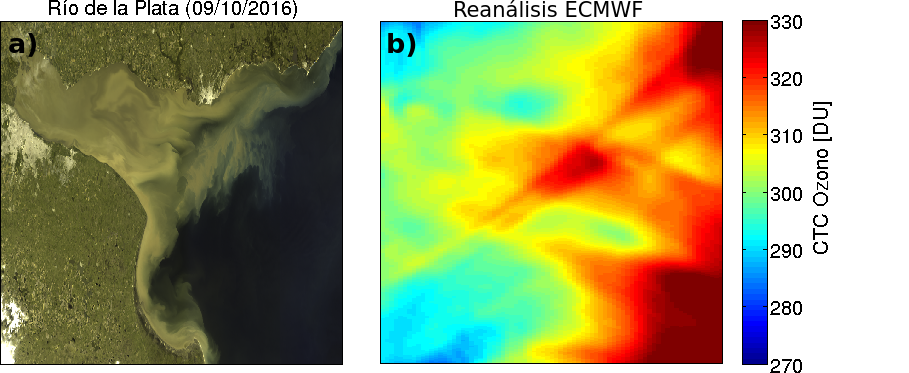
\includegraphics[width=\textwidth]{int/figures/O3_RDP_ECMWF.png}
    \caption[Concentración de ozono en DU obtenida del re-análisis de ECMWF para el RdP el día 09-OCT-2016.]{a) Composición RGB de OLCI (Sentinel-3A) del Río de la Plata del día 9 de octubre de 2016 (en geometría del sensor). b) Concentración de ozono en DU obtenida del re-análisis de ECMWF que es distribuido por la ESA dentro de los productos L1B.}
    \label{int:O3_RDP_ECMWF}
    \end{figure}

    \begin{figure}
    \centering
    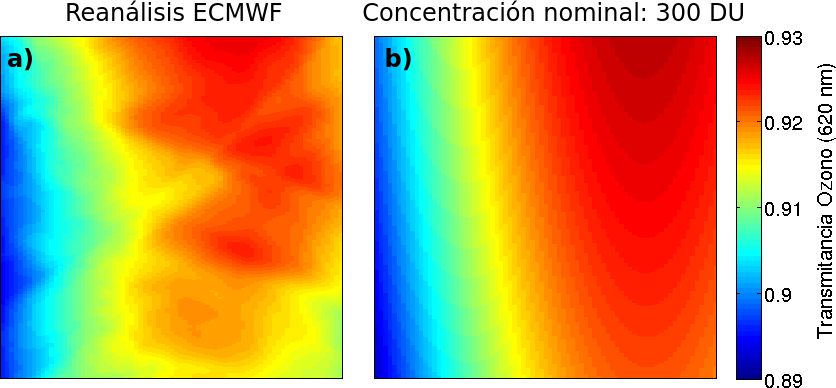
\includegraphics[width=\textwidth]{int/figures/O3_ECMWF_VS_NOM.png}
    \caption[Transmitacias debidas a la absorción del ozono a partir de concentración otorgada por ECMWF y de 300 DU (nominal).]{Transmitacias debidas a la absorción del ozono calculadas utilizando concentraciones provistas por el re-análisis de ECMWF (a) y una concentración nominal de ozono de 300 DU (b).}
    \label{int:O3_ECMWF_VS_NOM}
    \end{figure}

    Por otro lado, la Figura \ref{int:NO2} muestra el factor de transmitancia del $NO_{2}$ para las bandas del SABIA-Mar según diferentes concentraciones (CTC) y factores de masa ($\mu$). Obsérvese que, obviando las curvas asociadas al valor extremo de $[NO_{2}] = 6\times10^{16} part/cm^{2}$ (triángulos) que se corresponden a escenarios industriales donde existen niveles altos de $NO_{2}$ troposféricos, los escenarios naturales presentan valores superiores al $97\%$; por lo que es de esperar un error pequeño al asumir un valor nominal de $[NO_{2}] = 1.1\times10^{16} part/cm^{2}$ (asteriscos). Aparte, la expresión de la Ec. \ref{int:eq:tAbsExpKCTCMU_NO2} dejaría de ser válida en los escenarios con valores extremos de escenarios industriales debido a que la mayoría del $[NO_{2}]$ en estos casos se hallaría en las capas más bajas de la atmósfera.

    \begin{figure}
    \centering
    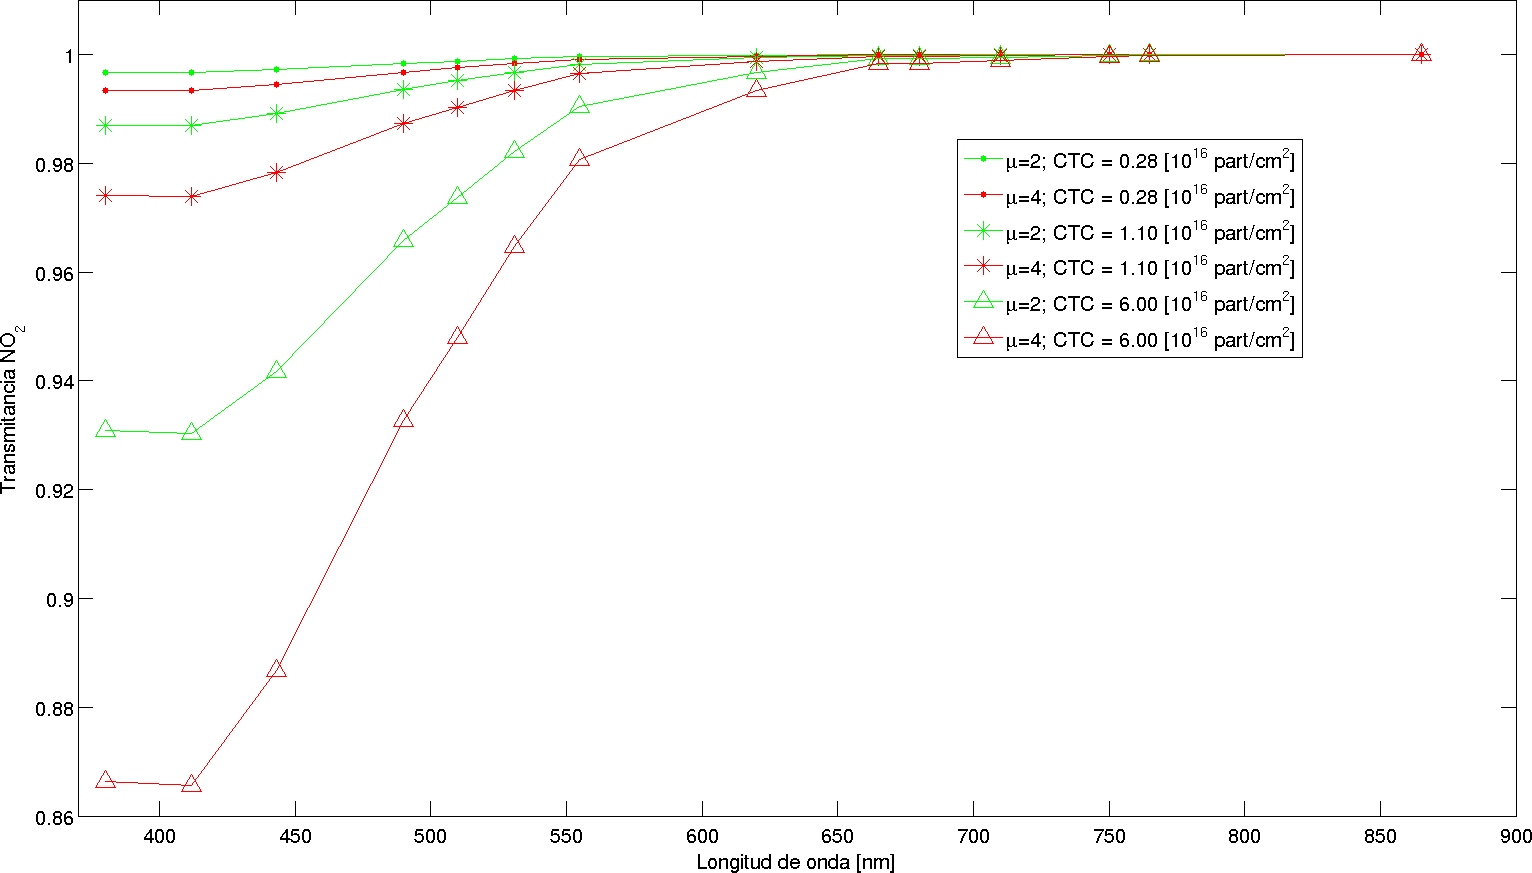
\includegraphics[width=\textwidth]{int/figures/NO2.png}
    \caption[Factor de transmitancia de NO$_{2}$ para diferentes concentraciones y factores de masa de aire.]{Factor de transmitancia de NO$_{2}$ para diferentes concentraciones y factores de masa de aire ($\mu$) para las bandas del SABIA-Mar.}
    \label{int:NO2}
    \end{figure}
    
    Cuando no se disponen de valores de concentración de gases absorbentes en la atmósfera, se pueden asumir los valores nominales de concentración de $O_{3}$ y $NO_{2}$ dados en las Ecs. \ref{int:eq:conc_o3} y \ref{int:eq:conc_no2}, como en Vanhellemont et al. 2014 \cite{vanhellemont2014}. De esta forma, y habiendo evadido las líneas de absorción de los gases troposféricos, se puede calcular un factor de transmitancia total gaseosa $t_{g}$ que sólo variará de acuerdo a la banda y al factor de masa ($\mu$):


    \begin{equation}
        t_{g}(\lambda) = t_{g}^{O_{3} + NO_{2}}(\lambda,\mu)
        \label{int:eq:tAbsO3NO2Nominal}
    \end{equation}

    En la Figura \ref{int:AbsorcionGaseosaHyper375_1700} se muestra la variabilidad hiper-espectral de la transmitancia gaseosa total en el rango $[375-1700]$ nm, y los valores ya integrados en las bandas del SABIA-Mar (Figura \ref{int:AbsorcionGaseosaSabiaMar}). En ambos casos, se hallan los valores obtenidos para factores de masa $\mu=2$ (observación e iluminación en cenit) y $\mu=4$ (observación e iluminación a $60\degree$ del cenit). 

    \begin{figure}
    \centering
    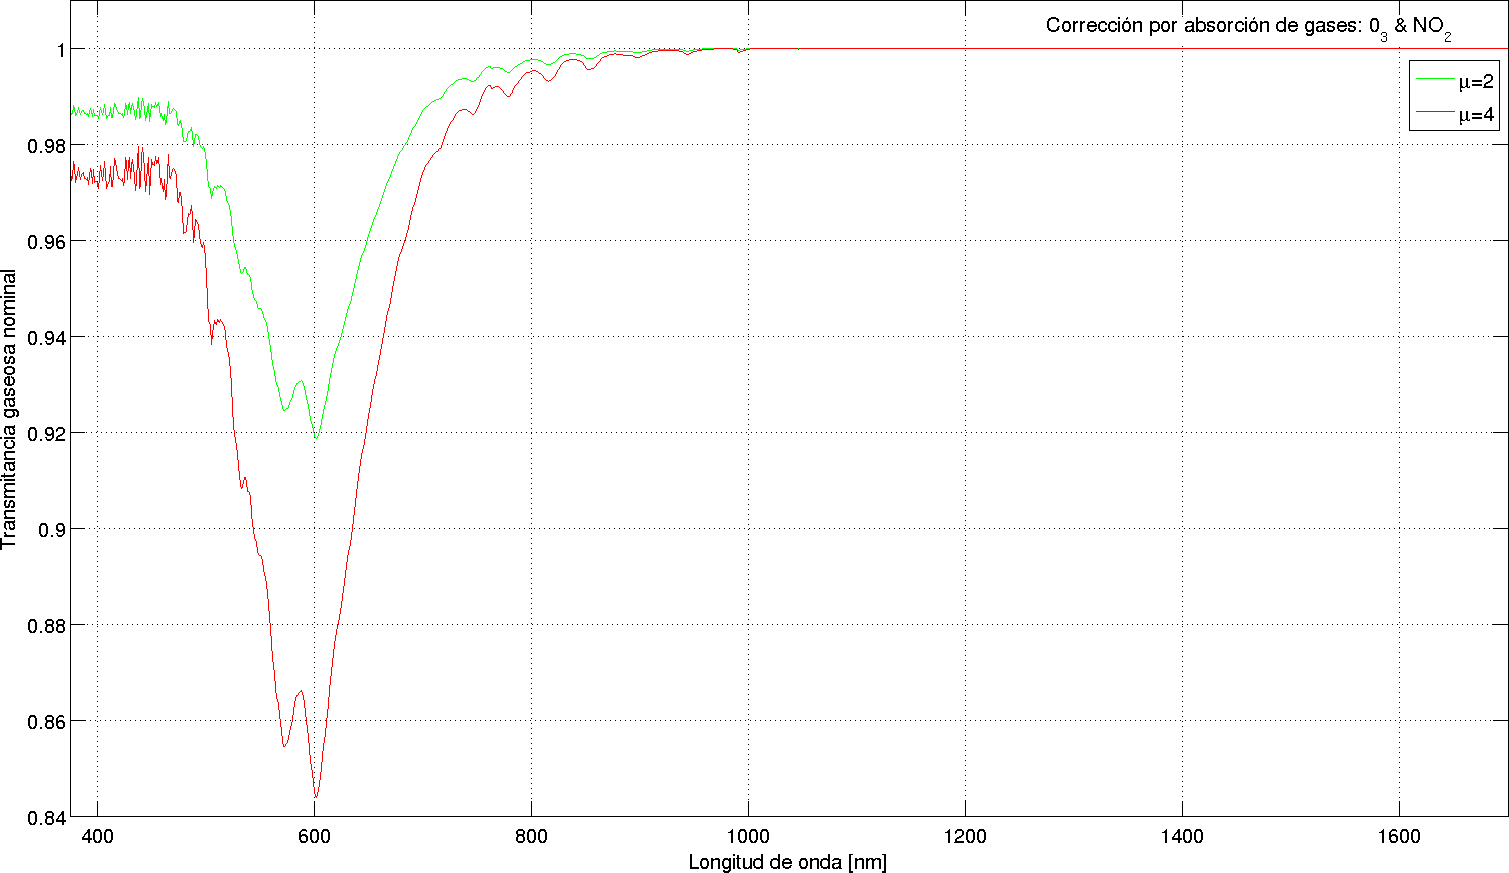
\includegraphics[width=\textwidth]{int/figures/AbsorcionGaseosaHyper375_1700.png}
    \caption[Transmitancia gaseosa por presencia de concentraciones nominales de ozono y dióxido de nitrógeno.]{Transmitancia gaseosa por presencia de concentraciones nominales de $O_{3}$ y $NO_{2}$ en el rango $[375-1700]$ nm: Valores obtenidos para factores de masa de aire $\mu = 2$ y $\mu = 4$.}
    \label{int:AbsorcionGaseosaHyper375_1700}
    \end{figure}

    \begin{figure}
    \centering
    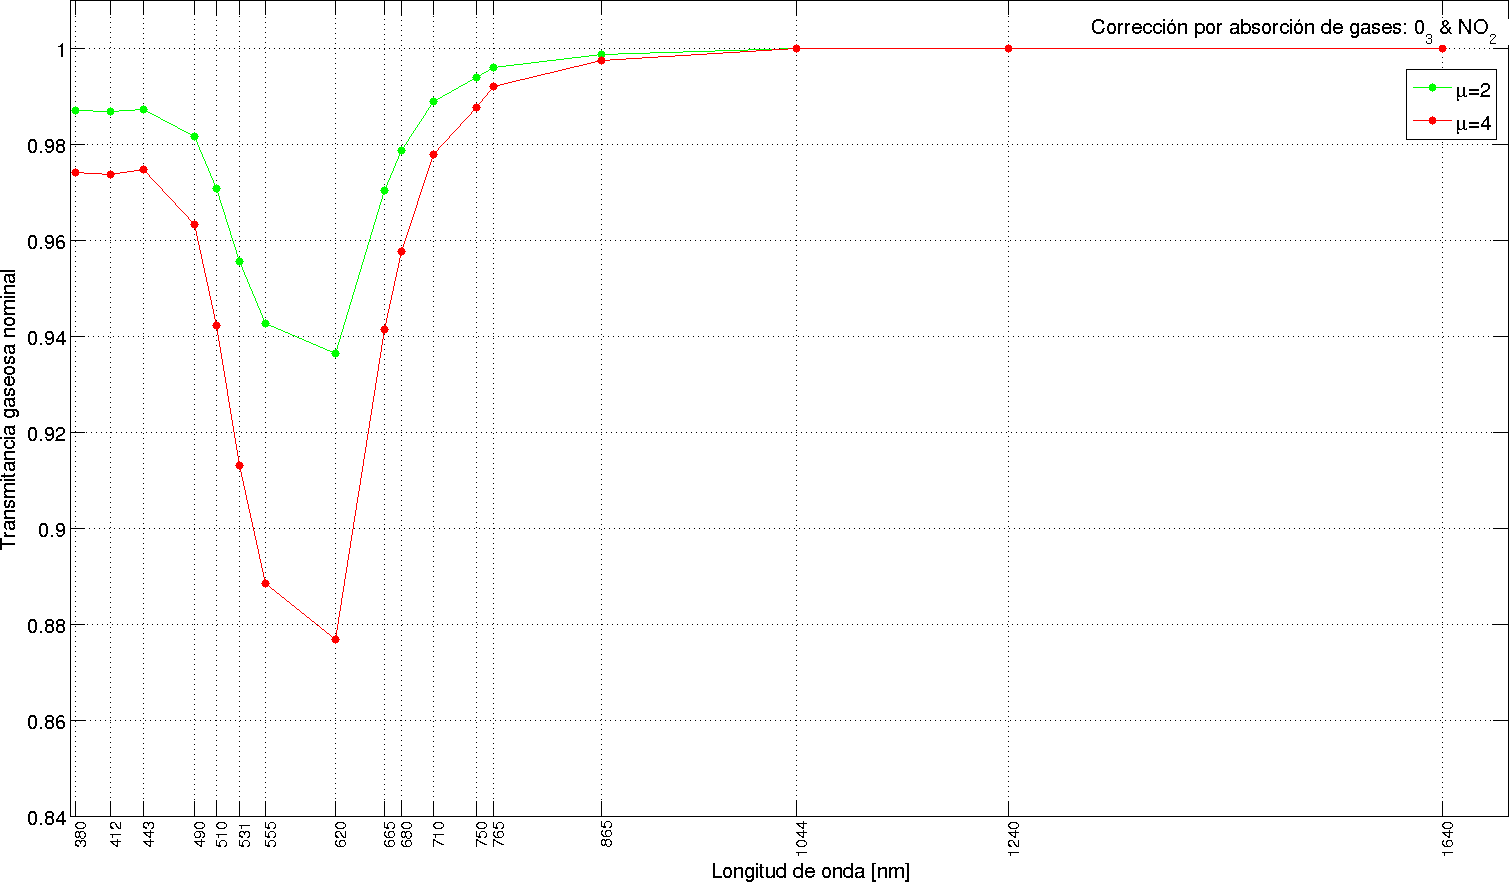
\includegraphics[width=\textwidth]{int/figures/AbsorcionGaseosaSabiaMar.png}
    \caption{Íd. Figura \ref{int:AbsorcionGaseosaHyper375_1700}, pero integrado sobre las SRFs de las bandas del SABIA-Mar.}
    \label{int:AbsorcionGaseosaSabiaMar}
    \end{figure}
    
\section{Dispersión Rayleigh molecular (B)}
\label{int:s:rayleigh}

    La dispersión de Rayleigh es la dispersión elástica de la luz visible o cualquier otra radiación electromagnética por partículas cuyo tamaño es mucho menor que la longitud de onda de los fotones dispersados. En la Teoría Clásica Electromagnética la dispersión de Rayleigh se genera como resultado de la polarizabilidad de las moléculas que actúan como centro dispersor. A partir de un campo de REM inducido por el efecto del campo REM incidente sobre las cargas de la partícula, las mismas actuarán como un dipolo eléctrico que oscilará a la misma frecuencia que la del campo incidente. La radiancia $L_{r} $ de la luz dispersada por una molécula de aire en un haz de luz de longitud de onda $\lambda$ y radiancia incidente $L_{0}$ viene dada por:

    \begin{equation}
        L_{r} = L_{0}{\frac {(1+cos^{2}(\Theta))}{2R^{2}}}\left({\frac{2\pi}{\lambda}}\right)^{4}\left({\frac{n^{2}-1}{n^{2}+2}}\right)^{2}\left({\frac{d}{2}}\right)^{6}
        \label{int:eq:Lray}
    \end{equation}

    \noindent donde $R$ es la distancia a la partícula, $\Theta$ es el ángulo de dispersión, $n$ y $d$ son el índice de refracción y el diámetro de la partícula, respectivamente. A partir del término $1+cos^{2}(\Theta)$, notamos que la dispersión de Rayleigh es simétrica y cuasi-isótropa (Figura \ref{int:scatteringTypes}). A su vez, notamos que la dispersión de Rayleigh es fuertemente dependiente de la longitud de onda ($\lambda^{-4}$).
    
    
    Si bien en ciertas circunstancias la radiancia de Rayleigh puede comprender entre el 50\% y el 90 \% de la radiancia total a TOA (Figuras \ref{int:RDP_TC_comparison_B_RHOGRC} y \ref{int:RDP_TC_comparison_B_RHO}), las propiedades ópticas de la dispersión de Rayleigh en la atmósfera son fácilmente calculables (con un error de $\sim 0.2\%$). En el contexto de la CA de imágenes de color del mar, para llevar a cabo la corrección por dispersión Rayleigh (\textit{Rayleigh Correction}, RC) se suelen utilizar simulaciones de Transferencia Radiativa (TR) para resolver la Ecuación Vectorial (polarizada) de Transferencia Radiativa (EVTR, \S \ref{sos:s:EVTR}) bajo la única presencia de moléculas dispersivas de aire y una superficie reflectora (que dará lugar al término de \textit{skyglint}). Dicho código de transferencia radiativa deberá incluir fenómenos de dispersión múltiple, polarización y un modelo de rugosidad de la interfase agua-aire. Típicamente, ésta se parametriza en función de la intensidad del viento, siguiendo la distribución de inclinaciones de facetas de la superficie propuesta por Cox y Munk 1954 \cite{coxmunk1954} (Figura \ref{int:coxmunk}):
    
    \begin{equation}
        g_{glitter}(\theta_{n},w) = \frac{1}{4\pi\sigma^{2}(w)cos^{2}(\theta_{n})}e^{-\left(\frac{tan(\theta_{n})}{\sigma(w)}\right)^{2}}
        \label{int:eq:coxmunk}
    \end{equation}
    
    \noindent siendo $\theta_{n}$ la orientación cenital de cada diferencial de superficie de agua - es decir, cada faceta -, $w$ la intensidad del viento en $m/s$ y $\sigma(w[m/s]) = 0.00300 + 0.00512w$.


    \begin{figure}
    \centering
    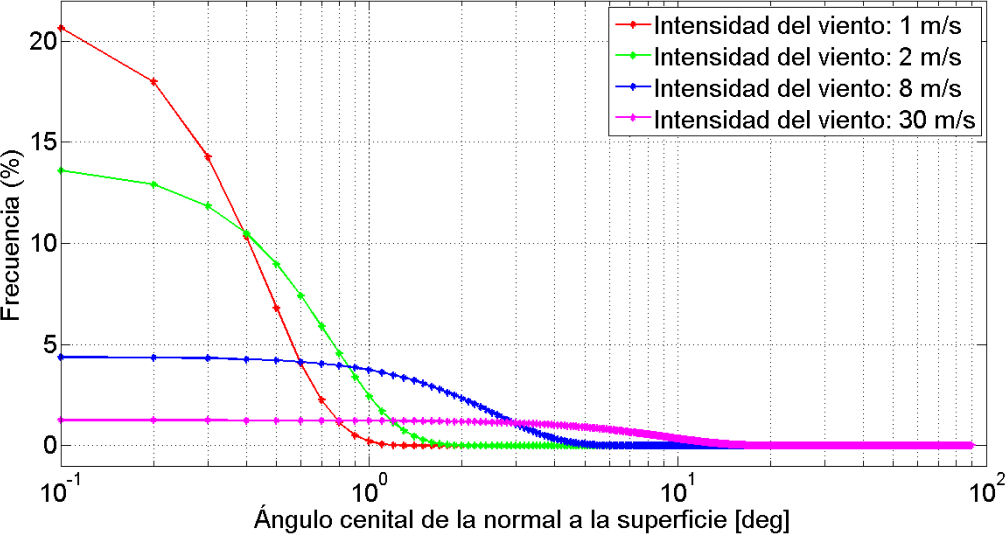
\includegraphics[width=\textwidth]{int/figures/coxmunk.png}
    \caption[Distribuciones de ángulos cenitales de las facetas de la interfase aire-agua para diferentes intensidades del viento en superficie.]{Distribuciones de ángulos cenitales formados por las direcciones normales de las facetas de la interfase aire-agua para diferentes intensidades del viento en superficie (Parametrización de Cox y Munk, \cite{coxmunk1954}). Un ángulo de $0\degree$ corresponde a una superficie horizontal. Paso de la distribución: $0.1\degree$.}
    \label{int:coxmunk}
    \end{figure}

    A su vez, para que el esquema de corrección por Rayleigh sea posible es necesario introducir los siguientes parámetros ópticos al código de transferencia radiativa:
    
    \begin{enumerate}
    
        \item \textbf{Cociente de depolarización molecular}, $\delta_{r}$. El mismo es una corrección debida a la anisotropía de las moléculas de aire. Este influye en las expresiones teóricas tanto de la matriz de fase (véase \S \ref{sos:s:matrizdefase}), inscripta dentro de la rutina de transferencia radiativa, como del espesor óptico. En general se utiliza la expresión dada por Bodhaine et al. 1999, \cite{bodhaine1999} (Figura \ref{int:rayleigh_tau_depol})
        
        \item \textbf{Espesor óptico molecular en superficie (Rayleigh)}, $\tau_{r}(\lambda, z = 0)$. El espesor óptico es el parámetro que indica la extinción de un haz de luz en una unidad de longitud dada (Ec. \ref{sos:eq:tau_definicion}). Existe una expresión teórica para el espesor óptico de Rayleigh, dada por \cite{bodhaine1999}:

        \begin{equation}
            \tau_{r}(\lambda, z = 0) = \frac{24 P N_{A}\pi^{3}(n^{2}-1)^{2}}{mg\lambda^{4}N^{2}(n^{2}-1)^{2}}\left(\frac{6+3\delta_{r}}{6-7\delta_{r}}\right)^{2}
            \label{int:eq:taur}
        \end{equation}

        \noindent siendo $n$ el índice de refracción del aire, $N$ la densidad molecular, $P$ la presión atmosférica en superficie y $N_{A}$ el número de Avogadro. El factor de la derecha (\textit{factor de King}) introduce la dependencia con $\delta_{r}$. Si bien esta expresión teórica es suficientemente adecuada para la corrección de Rayleigh aplicada a las imágenes de color, se utiliza típicamente el espectro reportado en Bodhaine et al. 1999, \cite{bodhaine1999} (Figura \ref{int:rayleigh_tau_depol}), al igual que el cociente de depolarización reportado por los mismos autores.

        \item \textbf{Altura característica de decaimiento exponencial}, $H_{r}$. En el cómputo de la reflectancia por dispersión Rayleigh, es necesario introducir la variación del espesor óptico molecular con la altura. Asumiendo una atmósfera isoterma y en balance hidrostático, el espesor óptico sigue un régimen exponencial decreciente con la altura:
    
        \begin{equation}
            \tau_{r}(\lambda, z) = \tau_{r}(\lambda, z = 0)e^{-z/H_{r}}
            \label{int:eq:hray}
        \end{equation}

        \noindent donde $z$ es la altura (en km) y típicamente, $H_{r} = 8$ km, siguiendo la ley barotrópica.
    \end{enumerate} 


    \begin{figure}
    \centering
    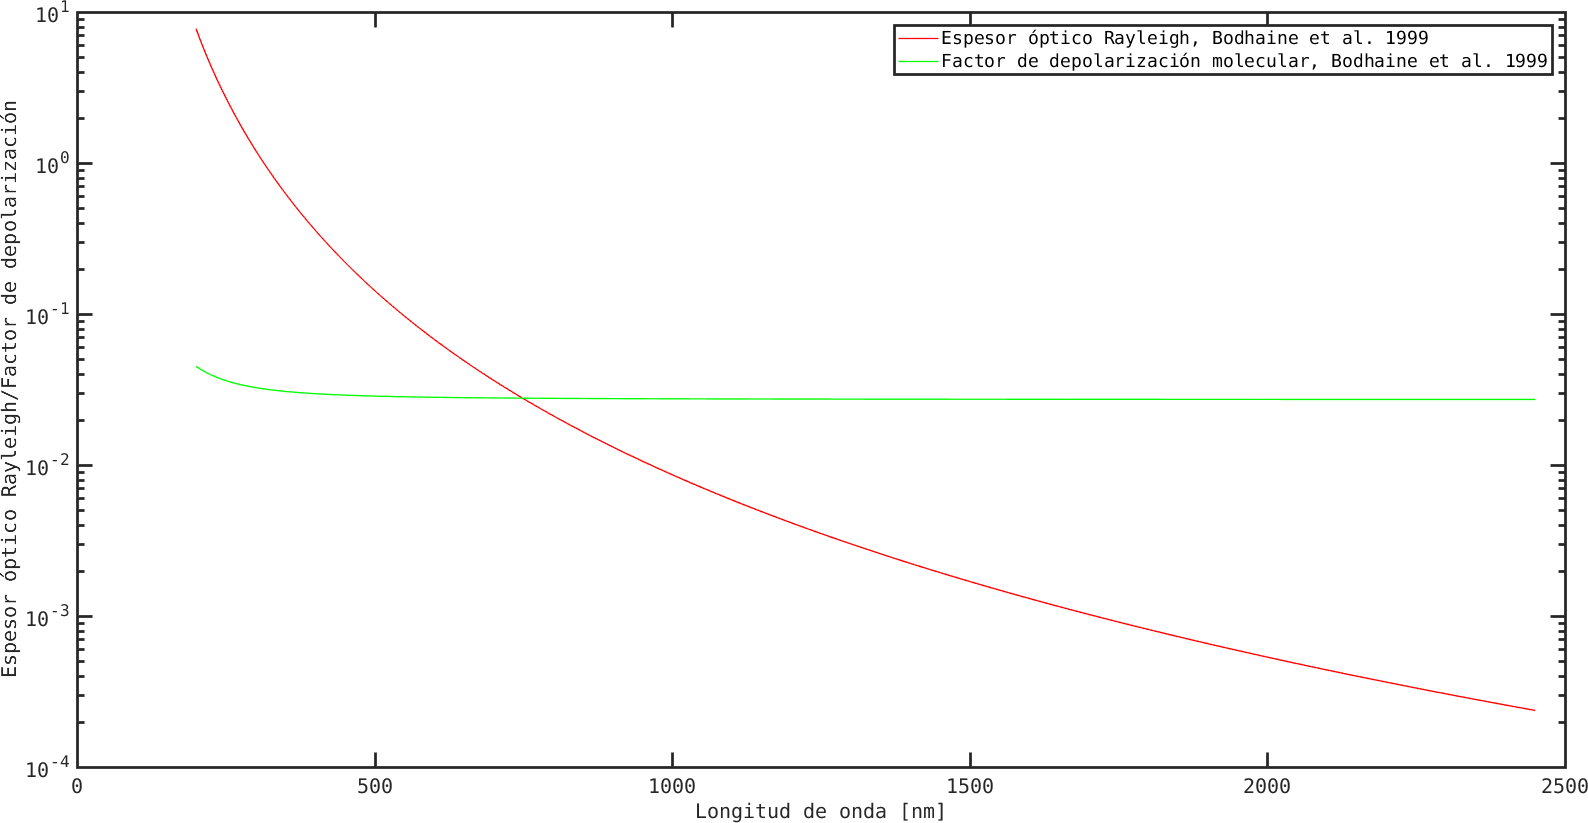
\includegraphics[width=\textwidth]{int/figures/rayleigh_tau_depol.png}
    \caption[Espesor óptico de Rayleigh y cociente de depolarización molecular.]{Espesor óptico de Rayleigh y cociente de depolarización molecular basados en Bodhaine et al. 1999, \cite{bodhaine1999}. [Graficado a partir del archivo bodhaine.txt que se halla en la página del OBPG de la NASA, \cite{obpg}].}
    \label{int:rayleigh_tau_depol}
    \end{figure}

    \begin{figure}
    \centering
    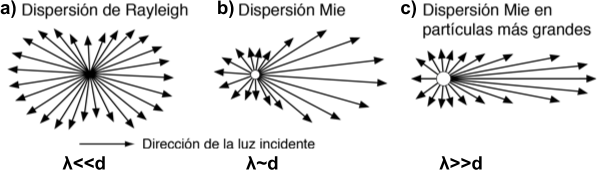
\includegraphics[width=0.75\textwidth]{int/figures/scatteringTypes.png}
    \caption[Distribución angular de la dispersión según la relación entre la longitud de onda y el tamaño de partícula.]{Distribución angular de la dispersión según la relación entre la longitud de onda ($\lambda$) y el tamaño de partícula ($d$): a) Dispersión tipo Rayleigh ($\lambda<<d$), b) tipo Mie ($\lambda \sim d$) y c) tipo Mie ($\lambda>>d$).}
    \label{int:scatteringTypes}
    \end{figure}

    En resumen, las reflectancias utilizadas para la corrección por Rayleigh (RC) se suelen obtener de tablas pre computadas (\textit{Look Up Tables}, LUTs) que dependen de los siguientes parámetros auxiliares:
    
    \begin{enumerate}
        \item Geometría de iluminación-observación (generalmente disponible con los productos satelitales).
        \item Velocidad del viento en superficie (necesaria para computar la rugosidad de la superficie, Ec. \ref{int:eq:coxmunk}).
        \item Presión atmosférica en superficie (necesaria para ajustar los valores de espesor óptico de Rayleigh, Ec. \ref{int:eq:taur})
    \end{enumerate}
    
    El detalle de cómo se efectúan estos cálculos en el procesador del OBPG de la NASA, SeaDAS (\textit{SeaWIFS Data Analysis System}) - utilizado en la presente tesis - se hallan descritos en Ahmad y Fraser 1982, \cite{ahmad1982}.

    \begin{figure}
    \centering
    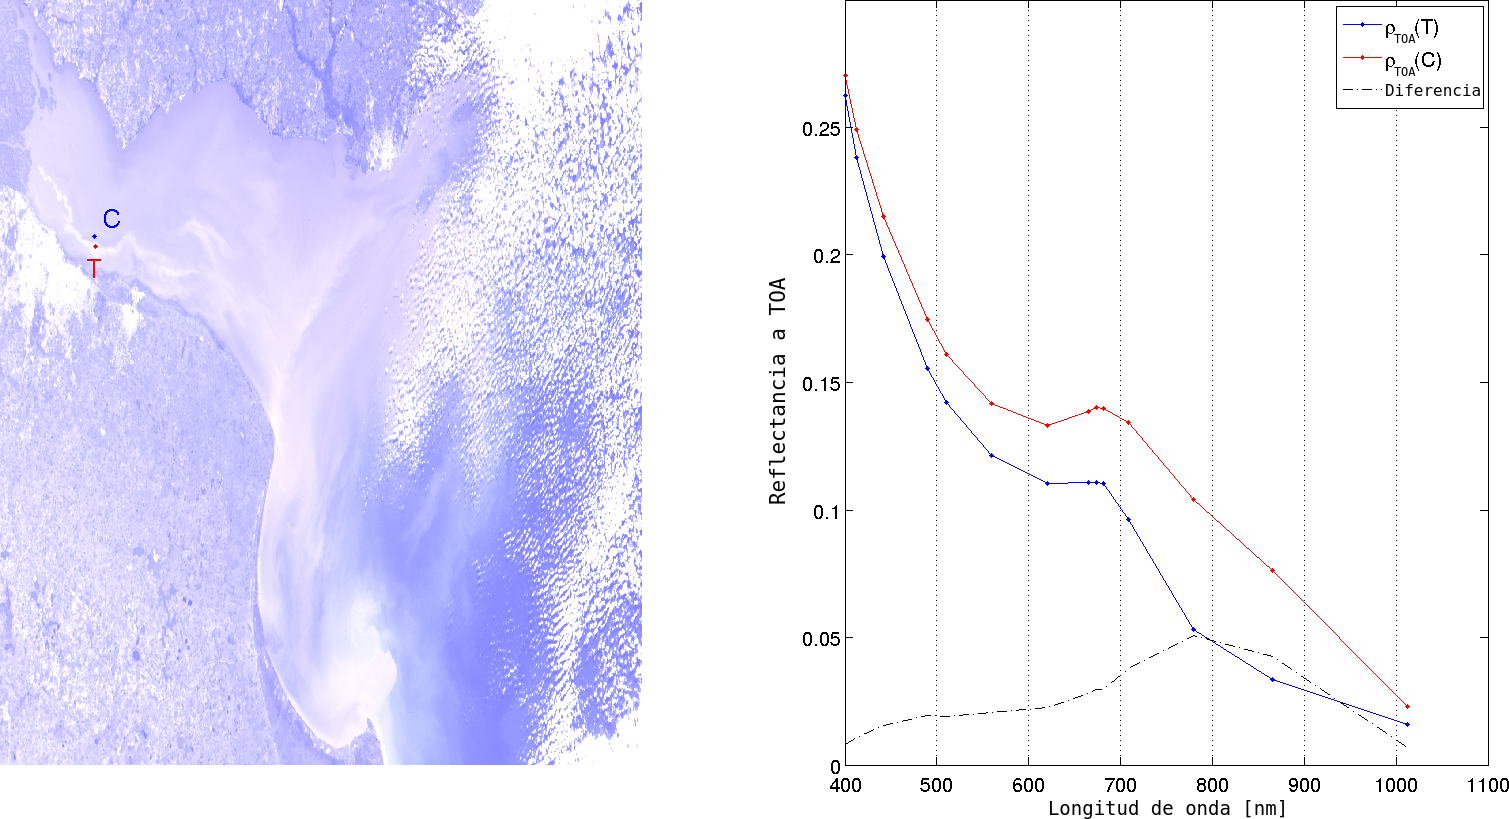
\includegraphics[width=\textwidth]{int/figures/RDP_TC_comparison_B_RHO.png}
    \caption[Reflectancia a TOA de la imagen de OLCI-A del 08-06-2016 sobre el RdP.]{Reflectancia a TOA ($\rho_{TOA}$, Ec. \ref{int:eq:rhotoa}) de la imagen de OLCI-A del 8 de junio de 2016 sobre el RdP. Izq.: Composición RGB - en geometría de sensor - observándose una fuerte componente azul proveniente de la dispersión Rayleigh. Der.: Reflectancias espectrales correspondientes a dos pines dentro de la imagen: \textit{T} (en aguas turbias del RdP) y \textit{C} (en aguas claras).}
    \label{int:RDP_TC_comparison_B_RHO}
    \end{figure}

    \begin{figure}
    \centering
    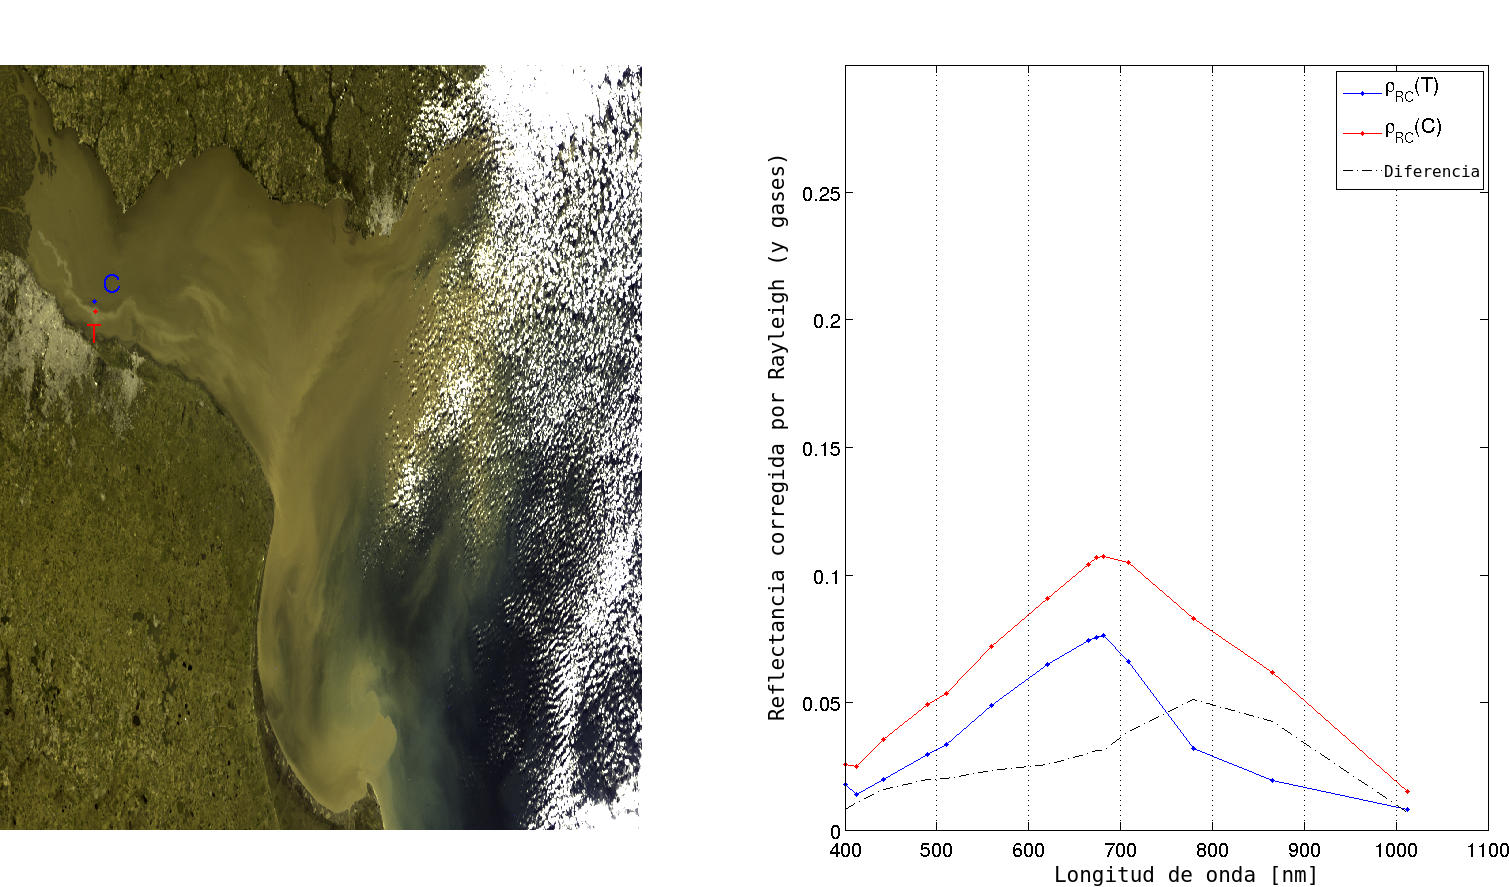
\includegraphics[width=\textwidth]{int/figures/RDP_TC_comparison_B_RHOGRC.png}
    \caption[Reflectancia RC de la imagen de OLCI-A del 08-06-2016 sobre el RdP.]{Ídem Fig. \ref{int:RDP_TC_comparison_B_RHO}, pero para reflectancia corregida por Rayleigh y por absorción de gases.}
    \label{int:RDP_TC_comparison_B_RHOGRC}
    \end{figure}

\section{Dispersión/absorción por Aerosoles (C)}
\label{int:s:aerosoles}

    Los aerosoles son partículas sólidas o líquidas que se hallan en la atmósfera, con tamaños característicos mucho mayores que las moléculas de gas - por lo cual sus propiedades dispersivas se enmarcan dentro del régimen de Mie (Figura \ref{int:scatteringTypes}) - pero a la vez lo suficientemente chicos como para mantenerse suspendidos en la atmósfera por períodos de horas, días o más \cite{mobley2016}. Los radios típicos varían dentro del rango $[0.1 - 10.0] \mu m$. Las propiedades ópticas de aerosoles son determinadas por su composición, la cual se parametriza usualmente a través de su índice de refracción (complejo) y su granulometría (o PSD, por \textit{Particle Size Distribution}). Para el propósito de la CA de imágenes de color es usual utilizar modelos de aerosoles (como los de Shettle y Fenn 1979, \cite{shettle1979}, los de la WMO, \cite{wmo1986} o los utilizados por la NASA de Ahmad et al. 2010, \cite{ahmad2010}) cuyas granulometrías resultan de la suma de dos modos: un modo \textit{fino} (de radios típicos del orden de $1 \mu m$) y uno \textit{grueso} (de radios mayores a $1 \mu m$). A su vez, es conocido que la granulometría de cada uno de estos modos sigue - en la gran mayoría de los casos - una distribución log-normal, por lo que, la distribución cumulativa en volumen resulta, teniendo en cuenta sendos modos: \cite{ahmad2010}
    
    \begin{equation}
        \frac{dV(r)}{d(lnr)} = \sum_{i=1}^{2}\frac{V_{0i}}{\sqrt{2\pi}\sigma_{i}}exp\left[-\left(\frac{ln(r)-ln(r_{v0i})}{\sqrt{2}ln(\sigma_{i})}\right)^{2}\right]
        \label{int:eq:aer_psd}
    \end{equation}
    
    \noindent donde $V(r)$ es el volumen total ocupado por las partículas con radio $r$, típicamente expresado en unidades de $\mu m^{3}cm^{-3}$; $r_{voi}$ y $\sigma_{i}$ son la media geométrica y el desvío estándar del radio del $i-$ésimo modo, respectivamente. Generalmente, el modo fino es de origen continental mientras que el grueso proviene de sales oceánicas.
    
    Las propiedades físicas de los aerosoles determinan sus propiedades ópticas: coeficientes de \textit{absorción} (\S \ref{qssa:s:a}),  \textit{dispersión} (\S \ref{qssa:s:b}) y \textit{función de fase} (\S \ref{sos:s:matrizdefase}). Típicamente - aunque no en todos los casos - es posible representar a los aerosoles como esferas homogéneas, lo que posibilita computar su impacto en el balance radiativo a partir de la Teoría de Mie, \cite{mishchenko2002}. Una vez que los coeficientes de absorción y dispersión específicos - $a^{*}(\lambda)$ y $b^{*}(\lambda)$ - y el perfil de concentraciones - $Conc(z)$ - de los aerosoles son conocidos, es posible computar el coeficiente de \textit{extinción}, $c(z,\lambda) = Conc(z)[a^{*}(\lambda) + b^{*}(\lambda)]$, \S \ref{qssa:s:c}. Luego, siguiendo lo expuesto en \S \ref{sos:s:bouguerlambertbeer}, es posible computar el espesor óptico de aerosoles:
    
    \begin{equation}
        \tau_{a}(\lambda) = \int_{z_{0}}^{TOA}c(z,\lambda) dz
        \label{int:eq:tau_aer_def}
    \end{equation}

    \noindent siendo $z_{0}$ la elevación de la interfase aire-agua (típicamente $z_{0}=0$ km para el Río de la Plata). Esto quiere decir que el espesor óptico de aerosoles en una determinada longitud de onda de referencia es proporcional a la concentración total de aerosoles. Luego, para extrapolar a otras longitudes de onda, es válido, dentro de un rango espectral suficientemente corto, utilizar una ley exponencial:
    
    \begin{equation}
        \tau_{a}(\lambda) = \tau_{a}(\lambda_{0})e^{-c_{\tau}(\lambda-\lambda_{0})}
        \label{int:eq:tau_aer_ang}
    \end{equation}

    \noindent donde $c_{\tau}$ es el coeficiente de decaimiento exponencial, o bien una ley de tipo Angstrom:
    
    \begin{equation}
        \tau_{a}(\lambda) = \tau_{a}(\lambda_{0})\left(\frac{\lambda_{0}}{\lambda}\right)^{\alpha_{\tau}}
        \label{int:eq:tau_aer_exp}
    \end{equation}

    \noindent donde $\alpha_{\tau}$ es el coeficiente de Angstrom. En general, aerosoles más pequeños (grandes) poseen coeficientes de Angstrom más grandes (pequeños), aproximándose al valor de $4$ en el límite de dispersión Rayleigh, Ec. \ref{int:eq:taur}.
    
    \subsection{Escenarios de aerosoles de la WMO}
    \label{int:s:wmo}
        Si bien existen varios catálogos de escenarios de aerosoles, nosotros describiremos muy brevemente los escenarios propuestos por la WMO, \cite{wmo1986}, dado que son los que están incluidos dentro del código de transferencia radiativa CNES-SOS utilizado en esta tesis (\S \ref{sos}). Los escenarios puros cuyos modos son log-normales son tres: el \textit{continental} (WMO-C), el \textit{marítimo} (WMO-M) y el \textit{urbano} (WMO-U) (Cuadro \ref{int:tab:wmo_CMU}). A su vez, cada uno de estos escenarios está conformado por distintas fracciones relativas de los modos de aerosoles de granulometría log-normal, a saber: \textit{polvos}, \textit{hidrosolubles}, \textit{oceánicos} y \textit{hollines} (Cuadro \ref{int:tab:wmo_modos}). 
        
        \begin{table}
        \caption[Proporción de cada componente de aerosoles según escenarios WMO.]{Proporción de cada componente de aerosoles según escenario propuesto por la WMO, \cite{wmo1986}.}
        \begin{tabular}{|l|l|l|l|l|}
        \hline
        \textbf{Escenario WMO} & \textbf{Polvo} & \textbf{Hidrosoluble} & \textbf{Oceánico} & \textbf{Hollín} \\ \hline
        \textbf{Continental}   & 70\%           & 29\%                  & 0\%               & 1\%             \\ \hline
        \textbf{Marítimo}      & 0\%            & 5\%                   & 95\%              & 0\%             \\ \hline
        \textbf{Urbano}        & 17\%           & 61\%                  & 0\%               & 22\%            \\ \hline
        \end{tabular}
        \label{int:tab:wmo_CMU}
        \end{table}

        \begin{table}
        \caption[Parámetros de las granulometrías de los modos log-normalres de aerosoles según reporte de la WMO.]{Parámetros de las granulometrías de los modos log-normalres de aerosoles según reporte de la WMO, \cite{wmo1986}.}
        \begin{tabular}{|l|l|l|}
        \hline
        \textbf{Tipo}         & \textbf{Radio medio [$\mu m$]} & \textbf{Desvío estándar [$\mu m$]} \\ \hline
        \textbf{Polvo}        & 0.5000                         & 2.99                               \\ \hline
        \textbf{Hidrosoluble} & 0.0050                         & 2.99                               \\ \hline
        \textbf{Oceánico}     & 0.3000                         & 2.51                               \\ \hline
        \textbf{Hollín}       & 0.0118                         & 2.00                               \\ \hline
        \end{tabular}
        \label{int:tab:wmo_modos}
        \end{table}

        \begin{figure}
        \centering
        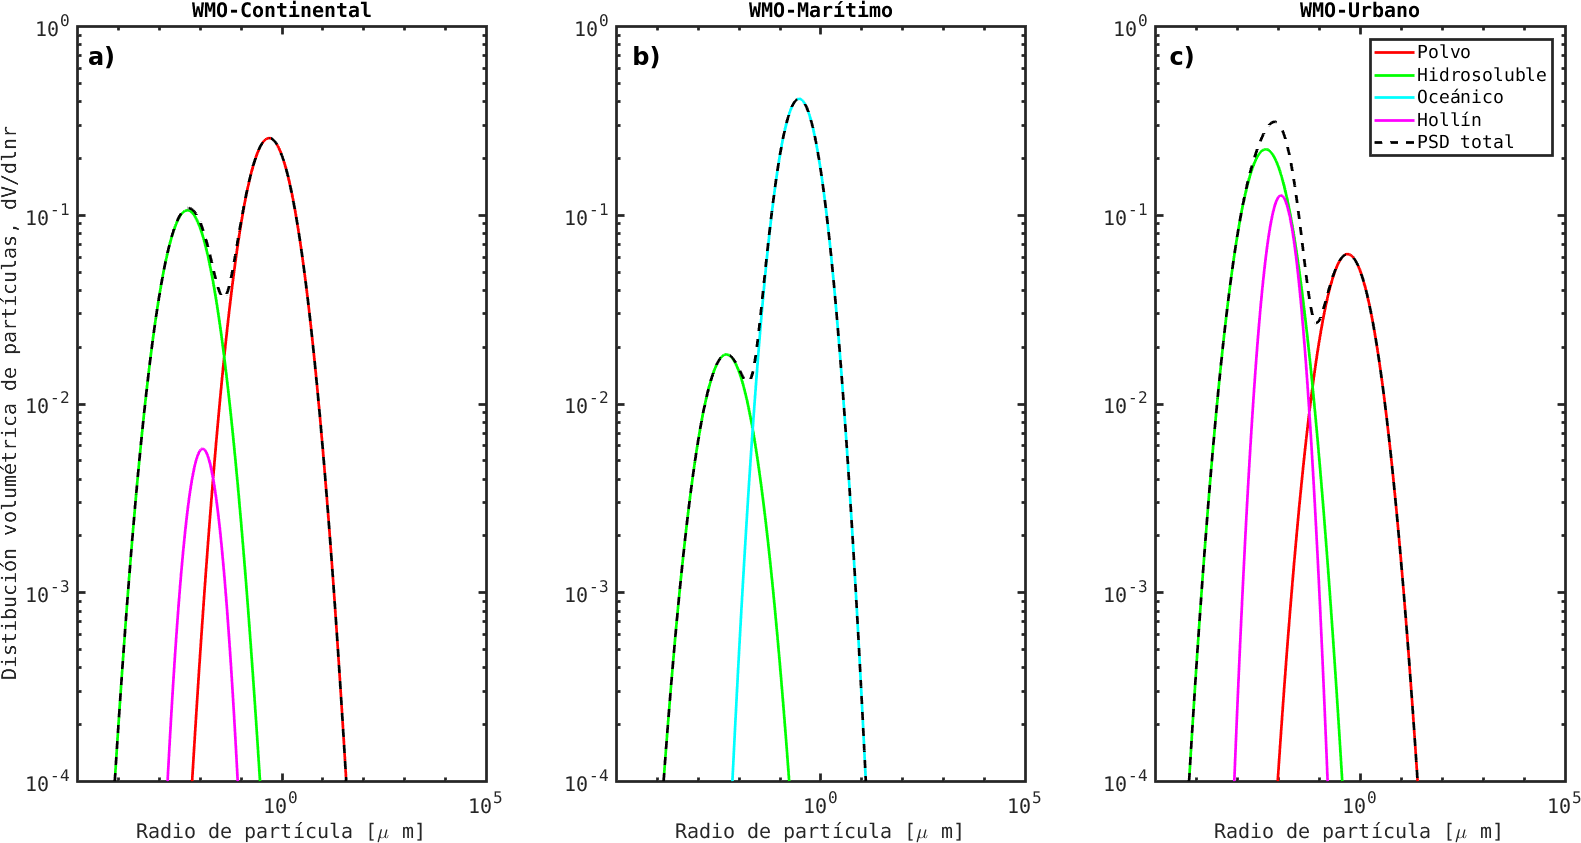
\includegraphics[width=\textwidth]{int/figures/WMO_PSD.png}
        \caption[Distibuciones granulométricas de los escenarios de la WMO.]{Distibución granulométrica, $dV/d(ln(r))$ (Ec. \ref{int:eq:aer_psd}), de los escenarios continental (a), marítimo (b) y urbano (c) propuestos por la WMO, \cite{wmo1986}.}
        \label{int:WMO_PSD}
        \end{figure}
        
        La información detallada de las propiedades de dichos modos de aerosoles (índice de refracción, albedo de dispersión simple, etc.) puede hallarse en \cite{wmo1986} y \cite{lafrance2002}.
    
    \subsection{Estrategias de cómputo de la reflectancia de aerosoles}
	\label{int:s:aer_estrategias}
    
        Contrario al caso de las moléculas de aire, los aerosoles son fuertemente variables en tamaño y composición, por lo que el cómputo de sus propiedades ópticas es más complejo que en el caso de la corrección por dispersión Rayleigh. Existen múltiples estrategias de corrección de aerosoles que podrán ser aplicables o no según el tipo de agua, atmósfera y sensor, de las cuales mencionaremos las principales \textit{familias}.
    
    	\subsubsection{Supuesto de agua negra en el NIR}
    	\label{int:s:ACblackPixelNIR}
    
            Dicho esquema fue desarrollado por Howard Gordon, \cite{gordon1978}\cite{gordon1980}\cite{viollier1980}\cite{gordon1981}\cite{gordon1987}\cite{gordon1988} culminando en el trabajo de Gordon y Wang 1994, \cite{gordon1994}, el cual plantea su aplicabilidad a imágenes SeaWIFS (que portaba dos bandas en el NIR centradas en $765$ nm y $865$ nm). El supuesto de agua negra se basa en el hecho de que la reflectancia proveniente del agua en la región del infrarrojo cercano (NIR) es prácticamente nula (véase Figura \ref{int:casoIyII}). Dicho fenómeno se debe principalmente a la fuerte absorción del agua líquida en dicha región del espectro, \cite{pope1997}\cite{kou1993}.

            Para entender cómo se aplica este supuesto, consideremos la \textit{reflectancia corregida por Rayleigh}, $\rho_{RC}$, que surge tras la corrección por absorción gaseosa, Rayleigh, \textit{sunglint} y \textit{whitecaps}:
            
            \begin{equation}
                \rho_{RC}:=\frac{\rho_{TOA}}{t_{g}}-\rho_{r}-T\rho_{g}-t\rho_{wc} = \rho_{a} + t\rho_{w}
                \label{int:eq:rhoResGW94}
            \end{equation}
            
            \noindent donde hemos expresado los términos de aerosoles como $\rho_{a}$ en vez de $[\rho_{a}+\rho_{ra}]$ por simplicidad. Si asumimos el supuesto de agua negra como válido podremos establecer que, dadas dos bandas en el NIR, $\lambda_{1}$ y $\lambda_{2}$:

            \begin{equation}
                \rho_{RC}(\lambda_{1,2}) \underbrace{=}_{\rho_{w}(\lambda_{1,2})=0} \rho_{a}(\lambda_{1,2})
                \label{int:eq:blackPixelAmplitud}
            \end{equation}

            \begin{equation}
                \epsilon(\lambda_{1},\lambda_{2}):=\frac{\rho_{RC}(\lambda_{1})}{\rho_{RC}(\lambda_{2})} \underbrace{=}_{\rho_{w}(\lambda_{1})=\rho_{w}(\lambda_{2})=0} \frac{\rho_{a}(\lambda_{1})}{\rho_{a}(\lambda_{2})}
                \label{int:eq:blackPixelEpsilon}
            \end{equation}
            
            De esta forma, con poseer al menos dos bandas donde el supuesto de agua negra sea válido es suficiente para establecer una amplitud y un parámetro de variabilidad espectral (tal como $c$ en la Ec. \ref{int:eq:tau_aer_exp} o $\alpha$ en Ec. \ref{int:eq:tau_aer_ang}) para la reflectancia de aerosoles. Luego, mediante la elaboración de LUTs de aerosoles, es posible extrapolar al resto de las bandas la señal de aerosoles determinada en las Ecs. \ref{int:eq:blackPixelAmplitud} y \ref{int:eq:blackPixelEpsilon}. Esto se hace eligiendo modelos de aerosoles - dentro de los que conforman las LUTs - cuyas características espectrales sean coincidentes con las de la reflectancia residual, $\rho_{RC}(NIR)$. Los pasos específicos de cómo es aplicado este esquema por el \textit{software} SeaDAS de la NASA a imágenes MODIS, SeaWIFS, VIIRS, etc. se hallan didácticamente detallados en Mobley et al. 2016, \cite{mobley2016}.

            Dicho esquema tiene dos contras fundamentales:
            
            \begin{enumerate}
                \item No es válido en aguas ópticamente complejas como las del RdP ya que el supuesto de agua negra no es válido en el NIR debido a la elevada retrodispersión de las partículas en suspensión. De hecho, este esquema será únicamente válido en aquellos escenarios donde las concentraciones de fitoplancton y sedimentos sean muy bajas. Afortunadamente, gran parte de las regiones oligotróficas de los océanos cumple dicha condición. En la Figura \ref{int:casoIyII} se muestran valores medidos de reflectacias del agua en escenarios muy contrastantes: el Río de la Plata - donde la reflectancia en el NIR es claramente no nula - y el Golfo San Matías - donde la reflectancia en NIR suele ser cercana a cero o nula.

                \begin{figure}
                \centering
                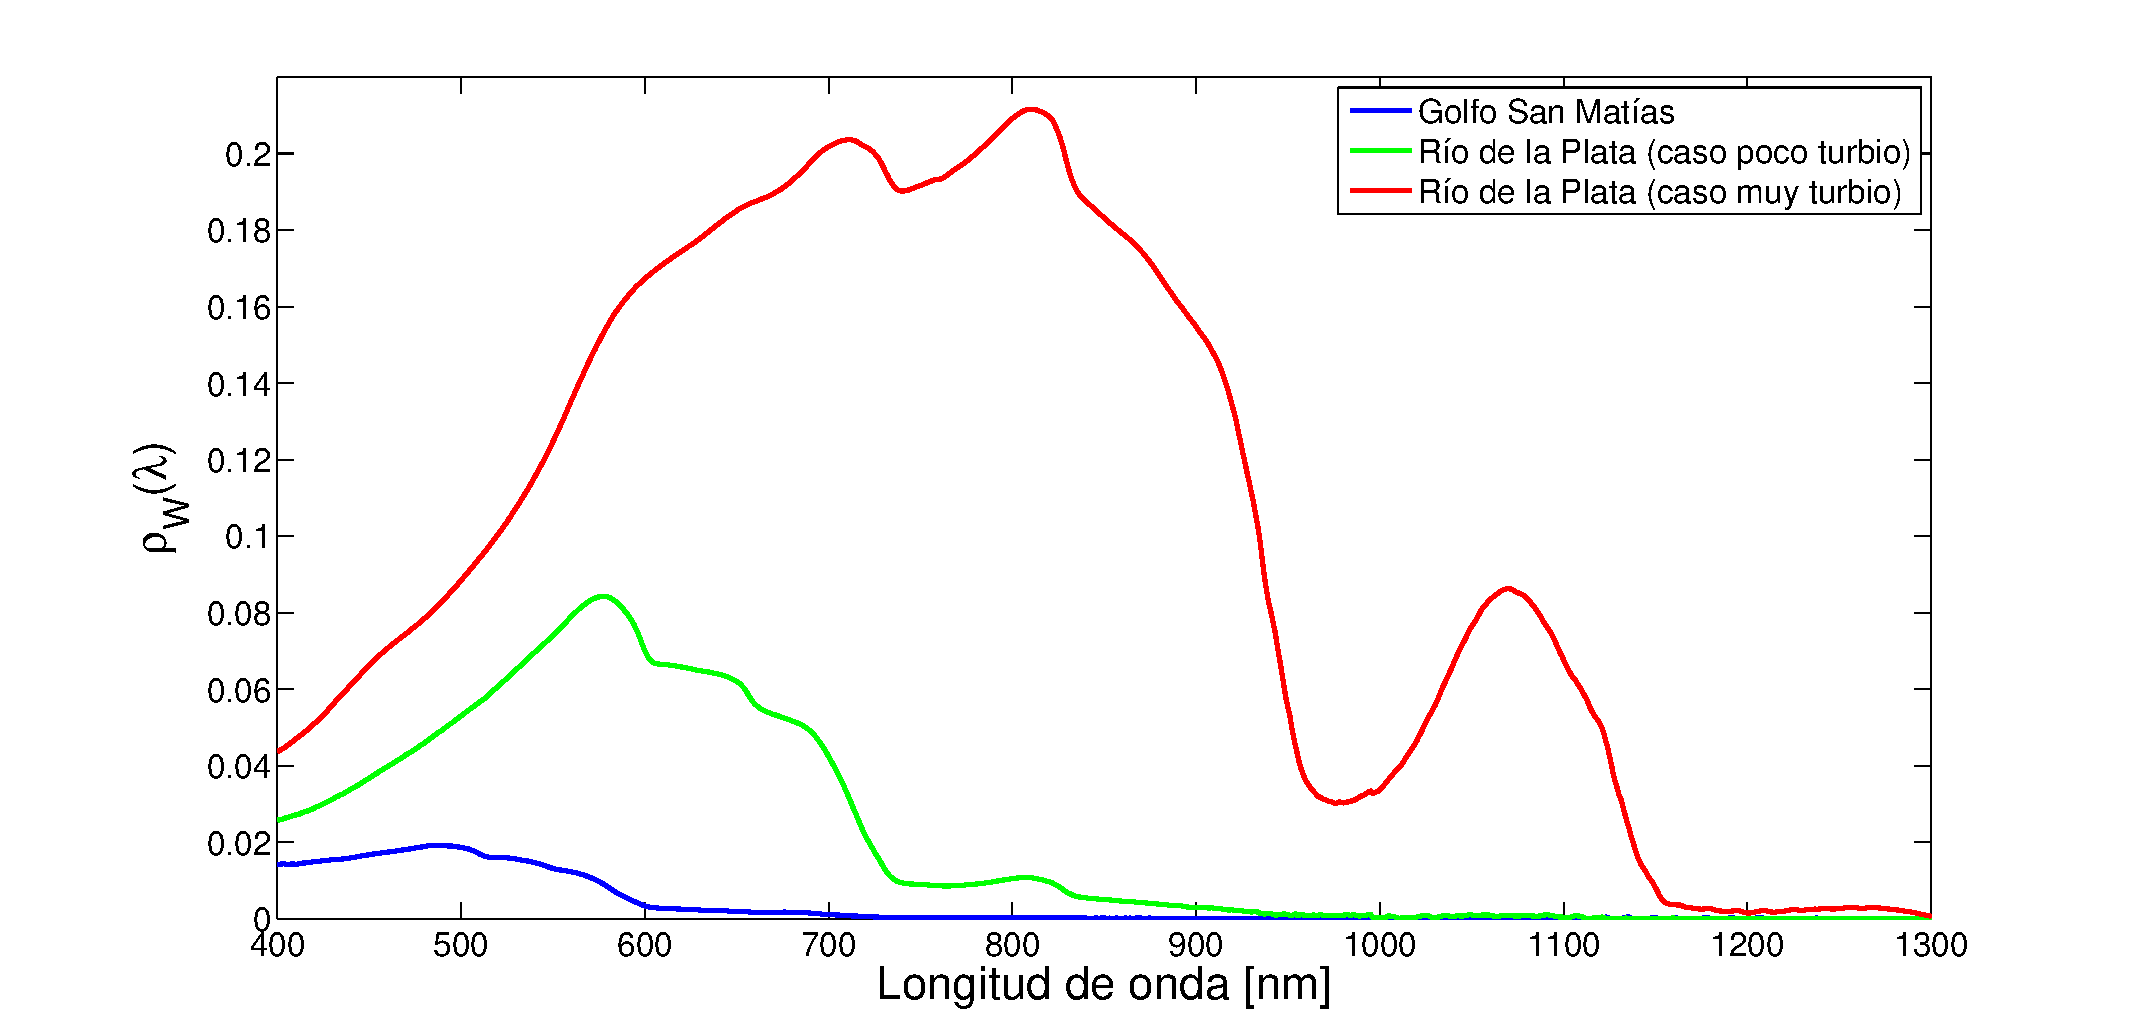
\includegraphics[width=1\textwidth]{int/figures/casoIyII}
                \captionof{figure}[Reflectancias de aguas claras y ópticamente complejas]{Reflectancias medidas sobre cuerpos de agua con características espectrales muy diferentes: el Río de la Plata, donde el supuesto $\rho_{w}(NIR)=0$ es generalmente inválido, y el Golfo San Matías, donde generalmente dicho supuesto es válido. Reflectancia del Golfo de San Matías: cortesía de Gabriela Williams (CENPAT/CONICET).}
                \label{int:casoIyII}
                \end{figure}

                \item Los errores de extrapolación son muy pronunciados en las bandas espectralmente alejadas al NIR: el violeta y el azul. Esto implica que un pequeño error en la determinación de la amplitud o $\epsilon(\lambda_{1},\lambda_{2})$ puede producir grandes errores en la magnitud de $\rho_{a}$ en el azul. A su vez, si consideramos aerosoles fuertemente absorbentes, la extrapolación al azul muchas veces no es biyectiva. Esto quiere decir que al mismo valor de $\epsilon(\lambda_{1},\lambda_{2})$ en el NIR pueden corresponder dos modelos de aerosoles con valores muy disímiles de $\rho_{a}$ en el azul. Es por esto que típicamente no se consideran modelos de aerosoles muy absorbentes en las LUTs utilizadas para dicho esquema de corrección. 
            \end{enumerate}

    	\subsubsection{Esquemas iterativos en el NIR}
    	\label{int:s:ACiterNIR}
    	    La familia de CAs que sucedieron a la de Gordon y Wang 1994, \cite{gordon1994}, plantean esquemas iterativos para poder determinar la señal - no nula - del agua en el NIR. El método perteneciente a esta familia que actualmente es implementado por el OBPG (\textit{Ocean Biology Processing Group}) es descrito en Bailey et al. 2010, \cite{bailey2010}, aunque fue propuesto originalmente por Siegel et al. 2000, \cite{siegel2000}, Stumpf et al. 2003, \cite{stumpf2003}.
    	    
    	    El esquema parte de una corrida inicial en la que se aplica el esquema de agua negra y se obtiene una reflectancia del agua inicial en las bandas del visible (VIS). Luego, a partir de esta reflectancia y utilizando un modelo bio-óptico, se calcula la reflectancia del agua en el NIR y se la sustrae a la señal residual, $\rho_{RC}(NIR)$. De esta forma, se asume que en este primer paso la reflectancia residual se ha aproximado a la condición de agua negra, Ecs. \ref{int:eq:blackPixelAmplitud} y \ref{int:eq:blackPixelEpsilon}. Luego se vuelve a aplicar el procedimiento para obtener una nueva reflectancia del agua en el VIS y en el NIR. Estos pasos se repiten típicamente hasta la convergencia de la estimación o hasta alcanzar un número de iteraciones máximo.
    	    
            Dicho esquema es muy efectivo en escenarios de aguas moderadamente turbias, pero es fuertemente dependiente de la plausibilidad del modelo bio-óptico utilizado para el cálculo de la reflectancia en el NIR. A su vez, la señal del agua es muchas veces lo suficientemente elevada como para saturar las bandas NIR de los sensores, \cite{dogliotti2011}. Existen varias variantes que se basan en esquemas iterativos en el NIR: por ejemplo, el esquema modificado de Wang et al. 2012, \cite{wang2012}, utilizado para GOCI (Geostationary Ocean Color Imager), o el esquema BPC (\textit{Bright Pixel Correction}) aplicado sobre OLCI, \cite{moore1999}\cite{moore2011}\cite{moore2017}\cite{lavender2005}, aunque esta última no depende de un modelo bio-óptico en el VIS.

    	\subsubsection{Supuesto de agua negra en el SWIR}
    	\label{int:s:ACswir}
    
            La generación de sensores que fue lanzada al espacio tras el SeaWIFS, (por ej. MODIS, VIIRS, OLI, MSI), tiene incoporadas aparte de las bandas en el VIS y el NIR, bandas en el SWIR lejano $[1200 - 2500]$ nm, donde la absorción del agua líquida es varias veces mayor que en el NIR. Esto implica que el supuesto de agua negra sigue siendo válido en esta región del espectro; aunque para el caso extremo del frente de turbidez del Río de la Plata, esta hipótesis comienza a vulnerarse también en la banda del SWIR centrada en $1240$ nm, \cite{knaeps2012}, por lo que este cuerpo de agua resulta un desafío aún mayor a la hora de aplicar una CA basada en las bandas del SWIR.

            El esquema de agua negra en el SWIR fue propuesto por Wang y Shi 2005, \cite{wang2005} y se resume a continuación:

            \begin{enumerate}
                \item Los valores de $\rho_{RC}(SWIR)$ son utilizados de manera equivalente que los casos de aguas claras, asumiendo agua negra en el SWIR, para obtener un modelo de aerosoles extrapolable a las bandas del NIR.
                \item Luego se obtienen, a partir de dicho modelo de aerosoles, los valores de $\rho_{w}(NIR)$.
                \item Finalmente, sustrayendo estos valores de $\rho_{w}(NIR)$ a $\rho_{RC}(NIR)$, el esquema se halla en las condiciones iniciales correspondiente a aguas claras, por lo que se puede proceder a la extrapolación desde el NIR hacia el VIS.
            \end{enumerate}
            
            La problemática esencial que tienen las bandas del SWIR es que su razón señal-ruido (SNR) suele ser menor que la SNR de las bandas NIR, sumado al hecho de que son espectralmente más distantes a las bandas del VIS. Esto implica que la extrapolación mediante LUTs posea aún mayores inconvenientes que en el caso anterior. Aparte, no todos los sensores poseen bandas en el SWIR lejano debido a su elevado costo (por ej. OLCI y MERIS).

    	\subsubsection{Algoritmo NIR-SWIR}
    	\label{int:s:ACnirswir}
    	    El algoritmo NIR-SWIR fue desarrollado por Wang y Shi 2007, \cite{wang2007} y en realidad resulta en la aplicación del algoritmo NIR o SWIR dependiendo del grado de turbidez del agua, determinado por un índice propuesto por Shi y Wang 2007, \cite{shi2007}. En caso de que dicho índice exceda un umbral de turbidez mínimo, se aplica el esquema SWIR, \S \ref{int:s:ACswir}; caso contrario, se procede al esquema NIR iterativo de Bayley et al. 2010, \S \ref{int:s:ACiterNIR}. Si bien dicho algoritmo es aplicable a muchos cuerpos de agua, posee todos los defectos combinados de los dos esquemas en los que se basa. A su vez, el índice de turbidez en el que se basa suele no ser plausible en aguas turbias como las del RdP.

        \subsubsection{Supuesto de homogeneidad espacial}
        \label{int:s:ACmumm}
            Esta familia de algoritmos se basa en la idea originalmente descrita en Ruddick et al. 2000, \cite{ruddick2000}. A continuación, haremos una breve descripción del esquema:
            
            \begin{enumerate}

                \item Habiendo determinado la reflectancia residual o corregida por Rayleigh, notamos que se tiene:
                \begin{equation}
                    \rho_{RC}(\lambda_{i})=\rho_{a}^{I}(\lambda_{i})+t^{I}(\lambda_{i})\rho_{w}(\lambda_{i})\quad \forall i=1,...,N
                    \label{int:eq:RUDD:rhoCORR}
                \end{equation}
                
                \noindent siendo $I$ el modelo de aerosoles a determinar, $i$ el número de banda del sensor y $N$ el número total de bandas de interés. Se asumirá por simplicidad que el sensor en cuestión es el SeaWIFS; por lo que $N=8$; las bandas corresponden al visible para $1<i<6$, mientras que $i=7,8$ son bandas en el NIR ($765$ nm y $865$ nm).
                
                \item También se conoce, una vez determinado el modelo de aerosoles $I$, el parámetro espectral $\epsilon$:
                \begin{equation}
                \epsilon(\lambda_{i},\lambda_{j})=\frac{g^{I}(\rho_{a}^{I}(\lambda_{i}))}{g^{I}(\rho_{a}^{I}(\lambda_{j}))}
                \label{int:eq:RUDD:epsilon}
                \end{equation}
    
                \noindent siendo $g^{I}$ la transformación casi-lineal que lleva $\rho_{a}^{I}$ a $\rho_{a,s}^{I}$.
                
                \item Esto implica un total de 15 ecuaciones (las 8 de la Ec. \ref{int:eq:RUDD:rhoCORR} y las 7 de la Ec. \ref{int:eq:RUDD:epsilon}) para 17 incógnitas (los 8 valores de $\rho_{a}$, los 8 valores de $\rho_{w}$ y el modelo de aerosoles a determinar, $I$). En el esquema de agua negra en el NIR, el sistema se cerraba con dos condiciones más, $\rho_{w}(\lambda_{i})=0\quad i=7,8$.

                \item En el trabajo de Ruddick et al. 2000 \cite{ruddick2000} se propone la \textit{hipótesis de homogeneidad espacial en la región del NIR}. La misma asume los parámetros $\alpha_{7,8}$ y $\epsilon_{7,8}$ como valores fijos en una región acotada alrededor de determinado píxel en la imagen, siendo
                            
                \begin{equation}
                    \begin{aligned}
                        \epsilon_{7,8}&=\frac{\rho_{a}(\lambda_{7})}{\rho_{a}(\lambda_{8})}\\
                        \alpha_{7,8}&=\frac{\rho_{w}(\lambda_{7})t(\lambda_{7})}{\rho_{w}(\lambda_{8})t(\lambda_{8})}
                        \label{int:eq:RUDD:alphaydelta}
                    \end{aligned}
                \end{equation}
                    
                Dichos valores pueden ser obtenidos por procesos de calibración de la región de la imagen (véase \cite{ruddick2000}) donde se asume válida la hipótesis de homogeneidad.
            \end{enumerate}
            
            El mayor problema de este método reside en el hecho de que, en muchas ocasiones, la asunción de homogeneidad espacial no es válida o bien es difícil estimar el rango espacial de validez. Aparte, el requerimiento de computar los valores de los parámetros $\alpha_{7,8}$ y $\delta_{7,8}$ para múltiples regiones reducidas de una imagen implica un agregado al costo computacional e imposibilitando la automatización del proceso.

        \subsubsection{Supuesto de agua negra en el UV}
        \label{int:s:ACUV}
            Dicho supuesto fue planteado por primera vez por He et al. 2012, \cite{he2012}, y es en principio aplicable en aguas con elevado contenido de detrito orgánico y partículas no algales en suspensión, donde la elevada absorción del dichas sustancias hace que la reflectancia del agua en el UV se aproxime a 0, $\rho_{w}(UV)=0$, de forma tal de que la reflectancia RC en dichas bandas permite mejorar la calidad de la extrapolación al VIS a partir de la información provista por las bandas NIR y/o SWIR.
            
            El problema de dicho esquema es la mayoría de los sensores remotos vigentes no poseen bandas en el UV, más allá de que las mismas suelen presentar problemas de calibración y ruido. A su vez, el supuesto es únicamente válido en escenarios turbios. Si bien se ha esbozado la hiótesis de que el supuesto del NIR podría eventualmente extenderse al violeta asumiendo un valor constante de reflectancia, $\rho_{w}(400 nm)=cte>0$ (supuesto de \textit{anclaje} en el violeta), dicha hipótesis no ha sido demostrada hasta el momento.

        \subsubsection{Esquemas acoplados de espectro completo}
        \label{int:s:ACacoplados}
            Existen varios algoritmos que utilizan toda la información espectral disponible para realizar la CA, distinto de los previamente mencionados - que únicamente utilizan algunas bandas posicionadas en regiones estratégicas del espectro. Los mismos utilizan modelos acoplados de las propiedades ópticas de la atmósfera y el agua basados en una optimización o un enfoque iterativo para obtener una combinación más adecuada de pares de reflectancias agua-aerosoles, como por ejemplo en Doerffer y Schiller 2007, \cite{doerffer2007}, Chomko y Gordon 2001, \cite{chomko2001}. Dichos enfoques incluso han logrado la remoción exitosa del \textit{sunglint}, señal intensa pero espectralmente simple (por ejemplo, POLYMER, Steinmetz et al. 2011, \cite{steinmetz2011}) y tienden a proporcionar espectros plausibles de reflectancia de agua, evitando - por condiciones de contorno preestablecidas - reflectancias negativas. Incluso han demostrando ser muy robustos para datos con sesgos de calibración. Entre estos esquemas también podríamos incluir las inversiones basadas en redes neuronales, como en el caso de Jamet et. al 2005, \cite{jamet2005}, o bien las basadas en inferencia bayesiana, como el algoritmo desarrollado en Frouin y Pelletier 2015, \cite{frouin2015}.
            
            A pesar del éxito de estos algoritmos en varias circunstancias, los mismos se respaldan en modelos ópticos tanto de la atmósfera como del agua demasiado simples y que muchas veces no son representativos de la realidad. Por otro lado, dada la complejidad subyacente, en caso de no producir buenos resultados, es difícil hallar el origen de la falla en la estimación en comparación con los esquemas extrapolativos clásicos.

\section{Transmitancia directa (D)}
\label{int:s:tDir}

    Dicha transmitancia se aplica a términos de superficie que puedan ser considerados especulares, como el caso del \textit{sunglint}, donde el camino recorrido por los fotones interactuantes con la superficie es aproximadamente proporcional al factor de masa de aire (Ec. \ref{int:eq:mu}) al igual que en el caso de absorción de gases estratosféricos. De esta forma, aplicando la Ley de Bouguer-Lambert-Beer, \S \ref{sos:s:bouguerlambertbeer}, obtenemos la siguiente expresión:
    
    \begin{equation}
        T = T_{s}T_{v} = e^{-\tau/cos(\theta_{s})}e^{-\tau/cos(\theta_{v})} = e^{-\tau \mu}
        \label{int:eq:tDir}
    \end{equation}
    
    \noindent donde $\tau$ es el espesor óptico total de la atmósfera debido a procesos dispersivos. Considerando a las moléculas de aire y los aerosoles, resulta entonces $T = e^{-(\tau_{r} + \tau_{a})\mu}$.
    
\section{Reflexión especular del sol o \textit{sunglint} (E)}
\label{int:s:sunglint}
    
    Dado que el índice de refracción relativo de la interfase agua-aire es prácticamente constante a lo largo del UV-VIS-NIR-SWIR ($n\approx 1.334$), y el hecho de que las reflectancias de la Ec. \ref{int:eq:rhotoa} están normalizadas por la irradiancia solar, el término de reflectancia de \textit{sunglint} es casi espectralmente constante - a excepción del esperable acople de dicha señal con la atmósfera, modelado por los términos de transmitancia directa y de absorción gaseosa. De hecho, Wang y Bailey 2001, \cite{wang2001}, modelan dicha señal - amén de la transmitancia - como una constante espectral cuya variabilidad angular está dada por la geometría de iluminación y la rugosidad de la interfase agua-aire, a su vez parametrizada por la intensidad del viento en superficie, $w$, siguiendo nuevamente la Ec. \ref{int:eq:coxmunk}:
    
    \begin{equation}
        T(\theta_{v},\theta_{v})\rho_{g} = T(\theta_{v},\theta_{v})c(\theta_{v},\theta_{v},w)
        \label{int:eq:rhoglint}
    \end{equation}
    
    \noindent donde $\partial c/\partial \lambda = 0$. Si bien originalmente el \textit{sunglint} está incluido en las LUTs utilizadas para la corrección Rayleigh, el efecto del mismo es usualmente removido de las mismas y tratado aparte. Aunque en la actualidad existen algoritmos que resuelven la señal del \textit{sunglint} en conjunto con la señal de aerosoles (tales como POLYMER, \cite{steinmetz2011}), en escenarios de \textit{sunglint} extremo la señal de esta componente es tan alta que típicamente los píxeles afectados deben ser enmascarados. Es por esto que en muchos casos los sensores remotos no apuntan directamente al nadir, sino que suelen ser rotados de forma tal de que el \textit{sunglint} no contamine el centro de las imágenes, sino - en los casos de sensores polares heliosincrónicos - únicamente la porción \textit{este} dentro de la franja de barrido, como fue el caso del SeaWiFS.

\section{Transmitancia difusa (F)}
\label{int:s:tDif}

    La tranmitancia difusa es más difícil de modelar que la directa, puesto que se aplica a términos de superficie \textit{aproximadamente} lambertianos ($\rho_{wc}$ y $\rho_{w}$), por lo que el espesor de atmósfera recorrido por la radiación resulta incierto. En esta tesis se utilizará la siguiente expresión, sugerida por Tanre et al. 1979, \cite{tanre1979}:
    
    \begin{equation}
        t = e^{-(\sum_{i}^{N}(1-\frac{b_{b,i}}{b_{i}})\tau_{i})\mu}
        \label{int:eq:tDif0}
    \end{equation}
    
    \noindent donde $b_{i}$, $b_{b,i}$ y $\tau_{i}$ son los coeficientes de dispersión y retrodispersión (Ecs. \ref{qssa:eq:b} y \ref{qssa:eq:bb}) y el espesor óptico debido a la dispersión de la especie $i-$ésima. En nuestro caso, aproximaremos el coeficiente de retrodispersión de los aerosoles como $b_{b,a} = \frac{1}{6}b_{a}$, \cite{tanre1979}, y apelando a la isotropía de la dispersión Rayleigh, la transmitancia difusa resulta

    \begin{equation}
        t = e^{-(\frac{5}{6}\tau_{a} + \frac{1}{2}\tau_{r})\mu}
        \label{int:eq:tDif}
    \end{equation}

    \noindent o bien directamente omitiremos el efecto de los aerosoles en dicha expresión. Para entender este factor en más detalle, véase \cite{mobley2016}.

\section{Reflectancia de espuma o \textit{whitecaps} (G)}
\label{int:s:whitecaps}

    El efecto óptico causado por la espuma en superficie puede ser aproximado por un término lambertiano espectralmente blanco para longitudes de onda menores a 600 nm cuya intensidad variará según la fracción de superficie abarcada por la espuma, $f$. En el procesador estándar de la NASA, dicha fracción se parametriza en función del viento en superficie, $w$, siguiendo a Stamska y Petelski 2003, \cite{stramska2003}:
    
    \begin{equation}
        f = 8.75\times 10^{-5}(w[m/s]-6.33)^3
        \label{int:eq:rhoWC_f}
    \end{equation}

    \noindent mientras que la expresión para la reflectancia de espuma normalizada a $f=1$, $\rho^{*}_{wc}(\lambda)$, proviene de Frouin et al. 1996, \cite{frouin1996}:
    
    \begin{equation}
        \rho^{*}_{wc}(\lambda) = \left\{ \begin{array}{lcc}
                     1 &   si &  \lambda \leq 600 nm \\
                     e^{-0.00175(\lambda-600)} &  si & \lambda > 600 nm\\
                     \end{array}
           \right.
        \label{int:eq:rhoWC_a}
    \end{equation}
    
    En esta tesis, no consideraremos en general el efecto procovado por la espuma, dado que trabajaremos con aguas turbias - es decir, más reflectivas - por lo que podremos despreciar el efecto de la espuma.
\section{Área de estudio}
\label{int:s:area}

    El Río de la Plata (RdP) es uno de los sistemas estuariales más grandes del mundo ($\sim 35000$ km$^{2}$) drenando la segunda cuenca más grande de América del Sur luego del Amazonas. Tiene una longitud de $270$ km y un ancho de más de $220$ km en su boca (Figura \ref{int:rdp}) y sus aguas son poco profundas ($<20$ m). Se estima que la cantidad de sedimentos que transporta varía entre $80$ y $160$ millones de toneladas por año, lo cual lo lleva a ser uno de los ríos más turbios del mundo con valores de SPM de $10$ a $500$ mg/l (\S \ref{dat}). El RdP se caracteriza por la presencia de una zona de máxima turbidez asociada a un frente salino donde se produce el encuentro del agua dulce del río y el agua salada del océano, \cite{guerrero1997}\cite{mianzan2001}. La posición de dicho frente está principalmente controlada por la batimetría coincidiendo su posición media con la Barra del Indio en el sector norte y con la isobata de $5$ m en la Bahía de Samborombón hacia el sur. La gran cantidad de sedimentos transportados por el RdP influye, entre otros, en los procesos sedimentológicos cuyo estudio y comprensión resulta importante para un número de aplicaciones en zonas costeras. Varios estudios respaldados en datos de color del mar se han realizado para determinar el área de influencia de la pluma de agua turbia del Río de la Plata sobre aguas costeras del Atlántico Sudoccidental adyacente al estuario \cite{carvalho2014}\cite{garcia2008}\cite{piola2004}\cite{piola2008}.
    
    \begin{figure}
    \centering
    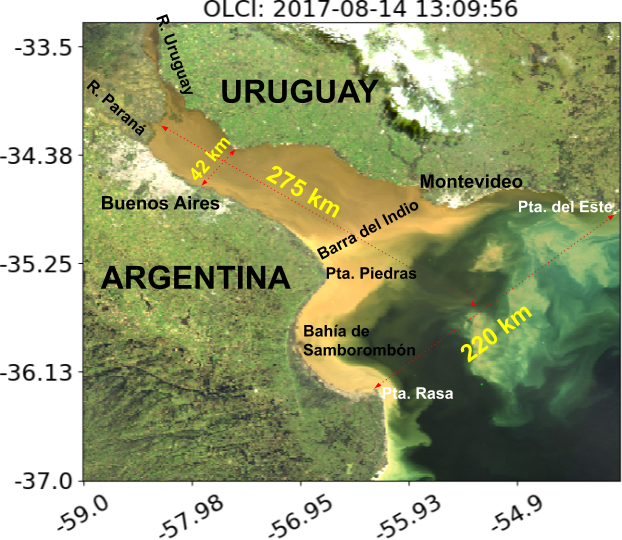
\includegraphics[width=\textwidth]{int/figures/rdp.png}
    \caption[Composición RGB del Río de la Plata.]{Composición RGB de la imagen OLCI del 14-AGO-2017 del Río de la Plata.}
    \label{int:rdp}
    \end{figure}

    Dadas las características particulares del RdP, gran superficie y alto SPM, esta región resulta un gran desafío y un área ideal para evaluar y desarrollar algoritmos de CA que permitan estimar la turbidez o concentración de  material en suspensión a partir de información satelital. En un primer estudio, Dogliotti et al. 2011, \cite{dogliotti2011} analizó en forma cualitativa el desempeño de tres algoritmos de CA aplicados a imágenes MODIS-Aqua en el RdP: i) el algoritmo de CA estándar de la NASA basado en las bandas NIR, \S \ref{int:s:ACiterNIR}; ii) el algoritmo NIR-SWIR, \S \ref{int:s:ACnirswir}, y iii) el algoritmo híbrido propuesto por Wang et al. 2011, \cite{wang2011} entre las estrategias NIR-SWIR y la de homogeneidad espacial, \S \ref{int:s:ACmumm}. Este estudio preliminar mostró - como era esperado - que el supuesto de agua negra en el NIR no se cumple en el RdP debido a la alta concentración de partículas en suspensión. A su vez, muestra que el procedimiento basado en el supuesto de agua negra en el SWIR tampoco genera buenos resultados para imágenes MODIS, puesto que muestra patrones espaciales correlacionados entre las reflectancias del agua y de aerosoles en la zona de máxima turbidez. Por último, si bien muestra buenos resultados para el esquema de Wang et al. 2011, este último posee las falencias propias de los esquemas basados en la homogeneidad espacial. Para otros sensores, como OLCI, se han visto resultados no satisfactorios para el esquema de CA estándar propuesto por la ESA (por lo menos hasta la versión 2.23, \S \ref{blr:s:results:blrac}).
    
    En resumen, estos resultados no concluyentes de las CA preexistentes evidencian la necesidad de realizar un análisis cuantitativo con datos radiométricos de campo y evaluar y/o desarrollar algoritmos alternativos.

\section{Objetivos}
\label{int:s:objetivos}
    La propuesta de tesis planteada propone como objetivo general mejorar la calidad de la información que se obtiene de sensores remotos a bordo de satélites con el fin de mapear la distribución espacio-temporal de variables biogeofísicas, como  la concentración de sedimentos en suspensión, en las aguas dominadas por sedimentos del Río de la Plata. En particular, se pretende llevar a cabo dicho objetivo mediante la exploración de nuevos esquemas de corrección atmosférica que mejoren las estimaciones de la reflectancia del agua en aguas turbias. El trabajo planteado contribuirá en forma directa a la misión argentino-brasileña SABIA-Mar por lo que varias de las simulaciones fueron realizadas para un sistema satélite-sensor con las características del propuesto para dicha misión. Con el fin de alcanzar el objetivo general se plantearon los siguientes objetivos específicos:
    
    \begin{enumerate}
    \item Continuar la colección de datos ópticos de reflectancia en muestras de agua de superficie en el Río de la Plata y organizar sistemáticamente los datos bio-ópticos en una base de datos. 
    \item Desarrollar algoritmos semi-empíricos para derivar la reflectancia del agua usando datos de campo y simulaciones de transferencia radiativa para SABIA-Mar y para diferentes sensores.
    \item Evaluar el desempeño de las correcciones atmosféricas desarrolladas.
    \item Desarrollar aplicaciones y potenciales productos del sensoramiento de color del mar sobre el área del Río de la Plata. 
    \end{enumerate}

\section{Descripción de la estructura de la tesis}
\label{int:s:estructura}

    Esta tesis está escrita en ocho capítulos:
    
    \begin{enumerate}
        \item En el capítulo \ref{int} se introdujeron los conceptos fundamentales de la teledetección del color del mar, de la corrección atmosférica y del área de estudio, con especial énfasis en aquellos que serán requeridos como bagaje previo a los capítulos posteriores.
        \item En el capítulo \ref{dat} se describirán las tareas de campo desarrolladas para calibrar/validar los algoritmos descriptos en los siguientes capítulos, así como un breve análisis de los datos de campo obtenidos. Por último se describirá la estructura de la base de datos confeccionada para sistematizar el almacenamiento y procesamiento de las mediciones realizadas.
        \item En el capítulo \ref{blr} se describirá el algoritmo BLR-AC desarrollado para aguas ópticamente complejas, específicamente para el conjunto de sensores OLCI, que carecen de bandas espectrales en el SWIR lejano, pero que poseen una novedosa banda en el SWIR cercano (1016 nm), que provee de información relevante para el proceso de remoción de aerosoles.
        \item En el capítulo \ref{pca} se describirá el algoritmo SWIR-PCA desarrollado para aguas ópticamente complejas del Río de la Plata para sensores como SABIA-Mar y MODIS que poseen bandas en la región espectral del SWIR lejano, es decir donde es válido el supuesto de agua negra para cualquier concentración de sedimentos.
        \item En el capítulo \ref{ppe} se describirá un procedimiento de corrección de las imágenes de OLCI y MERIS, necesario debido al efecto de eventos de partículas veloces que impactan en los sensores en la región Anomalía Magnética del Atlántico Sur - en particular, afectando las imágenes del Río de la Plata. Dicha corrección forma parte del preprocesamiento realizado previo a la corrección atmosférica descrita en el capítulo \ref{blr}.
        \item En el capítulo \ref{cam} se describirá una aplicación específica al estudio de imágenes de color del mar sobre las aguas ópticamente complejas como las del Río de la Plata: el algoritmo FAIT de detección de vegetación flotante en aguas turbias.
        \item En el capítulo \ref{oil} se describirá otra aplicación específica a estas imágenes: se describirá un posible algoritmo de detección de derrames de hidrocarburos en aguas turbias, junto con diversos índices que permitirían determinar el espesor de la capa superficial del derrame.
        \item En el capítulo \ref{con} se detallarán las conclusiones y las perspectivas a futuro de la presente tesis.
    \end{enumerate}
\chapter{Base de datos bio-ópticos de campo}
\label{dat}

\section{Introducción}
\label{dat:s:intro}

    La factibilidad y el poder predictivo de la mayoría de los algoritmos de estimación de variables biogeofísicas a partir de sensores remotos de color reside en gran parte en la disponibilidad de mediciones de campo de buena calidad de dichas variables. En general, tanto el alcance espacial como la plausibilidad de dichos algoritmos dependerá de la representatividad geográfica, la calidad y la cantidad de datos de campo que se disponga, por lo que el número total de mediciones requeridas suele ser grande. Esto implica que es fundamental mantener nuestro conjunto de datos de manera sistematizada y accesible.
    
    Una parte fundamental del trabajo de esta tesis consistió en adquirir, procesar y analizar datos de campo adquiridos principalmente en el estuario del Río de la Plata (RdP), aunque también en otras regiones. El volumen de datos de campo bio-ópticos disponibles para la región fue creciendo considerablemente desde el inicio de la presente tesis (los primeros datos radiométricos disponibles para la región corresponden a octubre del año 2012, medidos desde el Muelle del Club de Pescadores de Palermo, Buenos Aires), por lo que una tarea fundamental fue continuar con las tareas de campo y sistematizar la información obtenida en una base de datos. Si bien parte de estos datos fueron utilizados para el desarrollo de esta tesis, su recolección y sistematización trasciende los fines específicos de la misma, dado que dicha información es y será utilizada para continuar avanzando en la comprensión y el diseño de nuevos algoritmos en las aguas ópticamente complejas del estuario del RdP, así como de otras regiones de estudio que conforman parte de la base de datos.
    
    En este capítulo se describirán y analizarán las mediciones de campo realizadas en el marco de esta tesis, las cuales se realizaron durante campañas que perseguían objetivos específicos, ya sea en el marco de convenios o proyectos científicos o bien con la intención de documentar un evento puntual (por ejemplo, la invasión de plantas acuáticas superficiales en el verano de 2015/2016 en el RdP, \S \ref{cam}). En primer lugar, se describirán las áreas de estudio, los instrumentos utilizados, sus protocolos de medición y adquisición, sus protocolos de procesamiento y los criterios utilizados para la conformación de una base de datos sistematizada. Por otro lado, se analizará el comportamiento global obtenido para las principales variables bioópticas medidas en el RdP y se las comparará con los valores medidos en otras áreas estudiadas, cuyas aguas también son ópticamente complejas: el estuario del Río Tajo (Portugal) y la Laguna de Chascomús, en la Provincia de Buenos Aires.
   
\section{Características generales de las campañas}
\label{dat:s:generales}

    Durante las campañas se realizaron dos tipos de mediciones según su carácter temporal: o bien i) se midió de forma continua desde el inicio hasta el final de cada jornada de medición (por ejemplo, con el turbidímetro OBS501, ver \S \ref{dat:s:obs}), o bien ii) en forma discreta (estaciones) en horarios preestablecidos. Por otro lado, los horarios de las estaciones se determinaron fundamentamente (aunque no en todos los casos) siguiendo dos criterios fundamentales:
    
          \begin{itemize}
            \item La selección de fechas de medición depende fundamentalmente de i) las condiciones meteorológicas y ii) las pasadas de diferentes satélites de interés.
            \item  Generalmente se trata de realizar una estación simultánea para cada horario de adquisición de las imágenes satelitales de interés que estén disponibles para la jornada de medición. Dichas estaciones son las más relevantes para la validación de productos biogeofísicos satelitales (ejercicio de \textit{match up}).
            \item Fuera de los horarios de las pasadas se intentó generalmente que las estaciones se realizaran de manera periódica para intentar captar la variabilidad diaria del sitio durante la jornada de muestreo. Aún así, es en general impracticable obtener una periodicidad exacta para el muestreo por estación, dado que existen diversas causas de retrasos o adelantos en los tiempos de medición (advenimiento de una nube que perjudique las mediciones radiométricas, falla temporal de algún sensor, desperdicios flotantes en el agua que es necesario remover, etc.).
        \end{itemize}

\section{Áreas de estudio}
\label{dat:s:areas}

    Si bien la gran mayoría de las campañas realizadas como parte de la presente tesis - o bien dentro de nuestro grupo de investigación - tuvieron lugar en distintas regiones del RdP (descrito en \S \ref{int:s:area}), la base de datos total comprende información recopilada de varias otras regiones: los estuarios de los ríos Escalda (Bélgica), Girondo (Francia) y Tajo (Portugal), los golfos patagónicos de San Matías y San Jorge, la Estación Permanente de Estudios Ambientales (EPEA) frente a Mar del Plata y diversas lagunas bonaerenses. En el presente capítulo nos limitaremos a describir los resultados de los datos medidos en el RdP (Figuras \ref{dat:bardp} y \ref{dat:caba}) y a compararlos con el siguiente subconjunto de sitios:
    
    \begin{itemize}
    \item \textbf{Estuario del Río Tajo}: El estuario del Río Tajo se ubica en la costa oeste de Portugal y atraviesa la región urbana de su capital, Lisboa (Figura \ref{dat:tagus}). Cubre aproximadamente 320 km$^{2}$ y conforma una cuenca somera dominada por efecto de la marea que conecta con el Océano Atlántico mediante una profunda y estrecha entrada mareal (Guerreiro et al. 2015, \cite{guerreiro2015}). El lecho del estuario está compuesto principalmente por arenas y arcillas, ambas de origen fluvial y local; mientras que la boca y el canal intermareal están dominados por arenas de origen marino (Freire et al. 2007, \cite{freire2007}). Este estuario comparte con el RdP la característica de que sus aguas están ópticamente dominadas por la presencia de sedimentos inorgánicos en suspensión, aunque, a diferencia del RdP, las concentraciones de sedimentos son más bien moderadas. A su vez, suele presentar una fracción de material orgánico mayor a la del RdP. Estas similitudes y diferencias hacen interesante la comparación del comportamiento general de las variables bioópticas medidas en ambos estuarios.
    \item \textbf{Laguna de Chascomús}: la Laguna de Chascomús (Figura \ref{dat:chascomus}) es un cuerpo de agua turbia (hasta 300 FNU) debido a las altas concentraciones de fitoplancton (algas unicelulares, principalmente de los grupos de las cianobacetrias, \textit{Chlorophyceae} y \textit{Bacillariophyceae}) y material inorgánico (Sánchez et al. 2019, \cite{sanchez2018}). A diferencia del RdP, cuya aguas suelen presentar bajas concentraciones de fitoplancton, es de esperar que las reflectancias medidas en esta laguna presenten rasgos espectrales asociados a la absorción de los principales pigmentos que abundan en las células de dichos organismos.
    \end{itemize}
    
    \begin{figure}
    \centering
    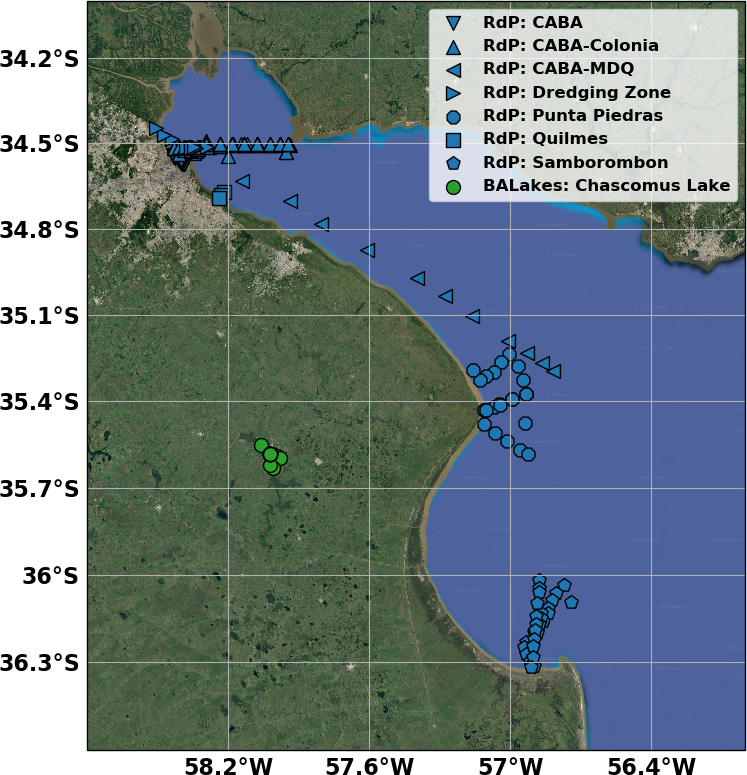
\includegraphics[width=\textwidth]{dat/figures/MAP_BARdp.png}
    \caption[Ubicación de las estaciones de campañas en la Provincia de Buenos Aires y el RdP.]{Ubicación de las estaciones de campañas en la Provincia de Buenos Aires y el RdP. El mapa resulta de una proyección \textit{Plate Carrée} del mosaico utilizado por la aplicación Google Maps, resultante de un ensamblado de representaciones RGB de imágenes ópticas de diversos satelites estadounidenses (de la serie LandSat) y europeos (del progama Copernicus). Naturalmente, el color azulado que se observa sobre el RdP no corresponde al color observado desde el espacio, sino que proviene de una máscara aplicada por Google Maps.}
    \label{dat:bardp}
    \end{figure}
    
    \begin{figure}
    \centering
    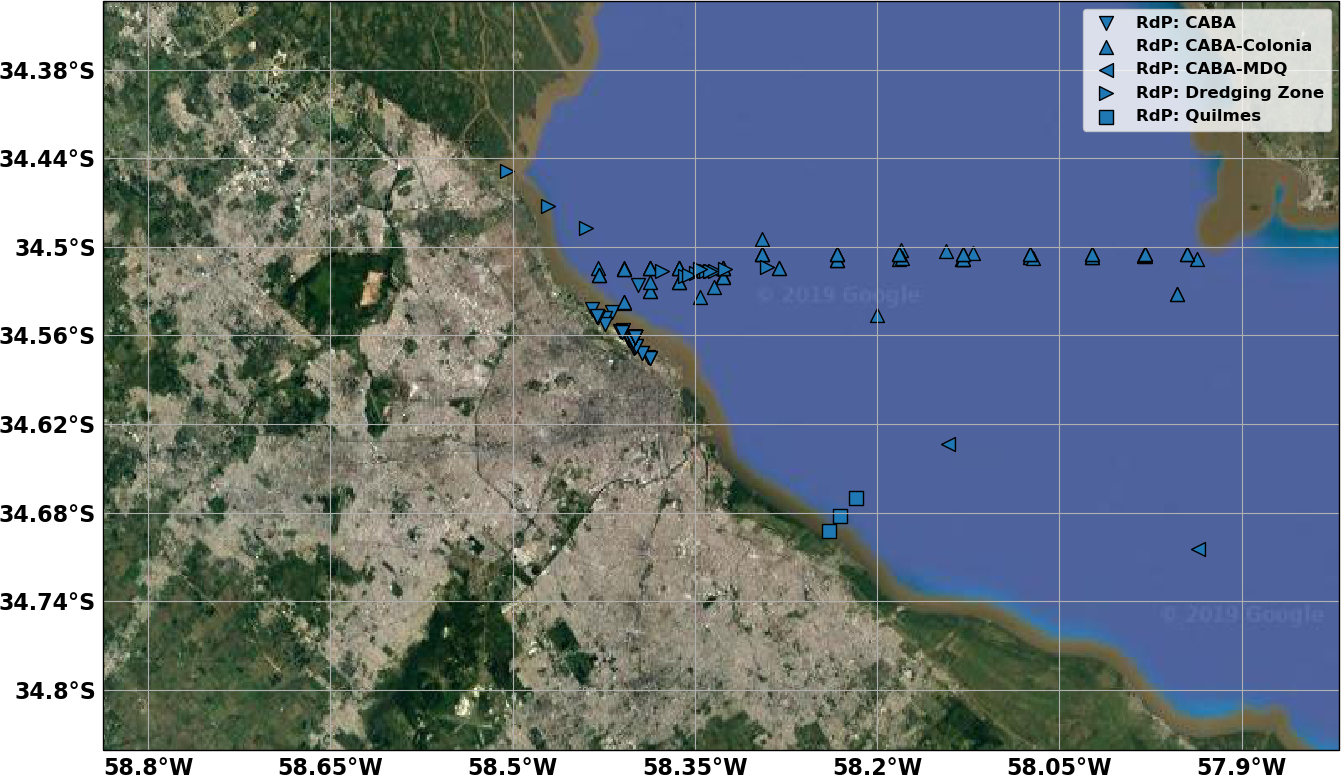
\includegraphics[width=\textwidth]{dat/figures/MAP_CABA.png}
    \caption[Ubicación de las estaciones de campañas en la región de la Ciudad de Buenos Aires.]{Ídem Figura \ref{dat:bardp}, ampliado en la región de la Ciudad de Buenos Aires.}
    \label{dat:caba}
    \end{figure}
    
    
    \begin{figure}
    \centering
    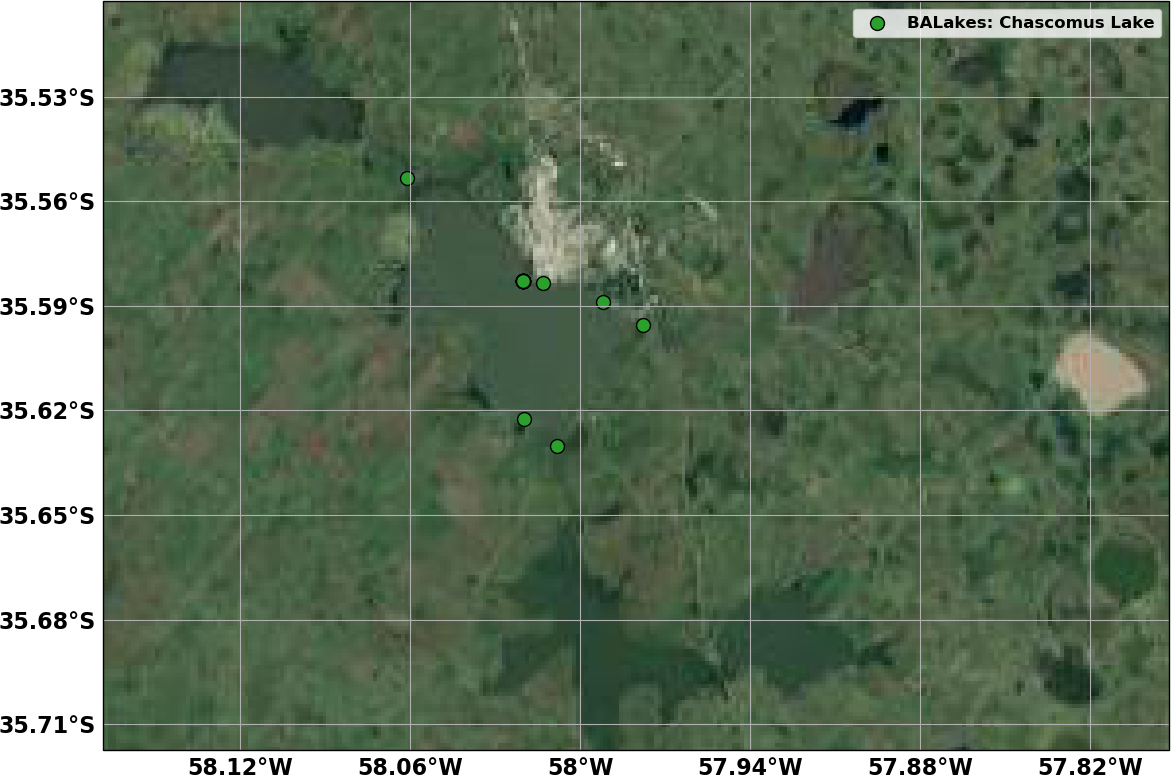
\includegraphics[width=\textwidth]{dat/figures/MAP_Chascomus.png}
    \caption[Ubicación de las estaciones de campañas en la región de la Laguna de Chascomús.]{Ídem Figura \ref{dat:bardp}, ampliado en la región de la Laguna de Chascomús (Chascomús, Prov. Buenos Aires).}
    \label{dat:chascomus}
    \end{figure}
    
    \begin{figure}
    \centering
    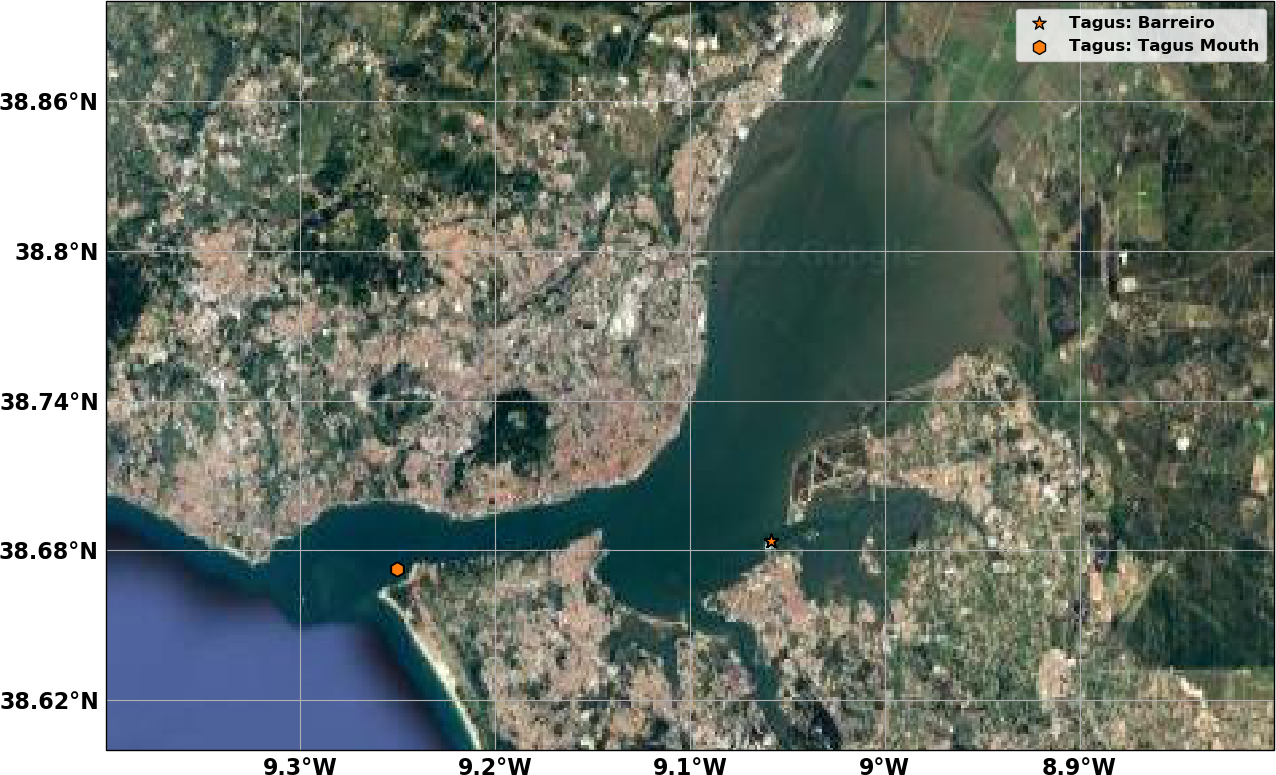
\includegraphics[width=\textwidth]{dat/figures/MAP_Tagus.png}
    \caption[Ubicación de las estaciones de campañas en la región del Estuario del Río Tajo (Portugal).]{Ídem Figura \ref{dat:bardp}, pero para las estaciones de campañas en el Estuario del Río Tajo (Lisboa, Portugal).}
    \label{dat:tagus}
    \end{figure}
    
    El Cuadro \ref{dat:tab:inventario} resume las campañas e instrumentos considerados en el presente capítulo [mediciones de la base de datos realizadas en otras regiones o con otros instrumentos fueron omitidas por exceder los objetivos de la presente tesis]. Obsérvese que los códigos identificatorios de cada campaña siguen el formato Región\_aaaammdd (año-mes-día), y que las siglas \textit{RdP}, \textit{BALakes} y \textit{Tagus} son los códigos identificatorios del RdP, las lagunas bonaerenses (dentro de las cuales se halla la de Chascomús) y el Río Tajo, respectivamente. A su vez, el Cuadro \ref{dat:tab:siglas} hace una breve descripción de las mediciones consideradas.
    
    \begin{table}
    \caption[Inventario del subconjunto de campañas analizado.]{Inventario del subconjunto de campañas caracterizado y analizado en este capítulo. Número de estaciones realizadas para cada uno de los instrumentos utilizados en cada una de las campañas [ver Cuadro \ref{dat:tab:siglas} para una breve descripción de cada instrumento].}
    \small
    \begin{tabular}{|l|c|c|c|c|c|}
    \hline
    \textbf{ID de campaña}                            & \textbf{ASD}             & \textbf{Trios}           & \textbf{OBS501}          & \textbf{SPM}             & \textbf{HACH}            \\ \hline
    \textbf{Región\_yyyymmdd}                         & \cellcolor[HTML]{000000} & \cellcolor[HTML]{000000} & \cellcolor[HTML]{000000} & \cellcolor[HTML]{000000} & \cellcolor[HTML]{000000} \\ \hline
    {\color[HTML]{009901} \textbf{BALakes\_20170131}} &                          & 1                        & 5                        & 1                        & 8                        \\ \hline
    {\color[HTML]{009901} \textbf{BALakes\_20170504}} &                          & 5                        & 5                        & 2                        & 3                        \\ \hline
    {\color[HTML]{009901} \textbf{BALakes\_20180409}} &                          & 5                        & 5                        & 5                        & 5                        \\ \hline
    {\color[HTML]{009901} \textbf{BALakes\_20190321}} &                          & 9                        & 11                       & 2                        & 11                       \\ \hline
    {\color[HTML]{3166FF} \textbf{RdP\_20120515}}     &                          &                          &                          & 13                       &                          \\ \hline
    {\color[HTML]{3166FF} \textbf{RdP\_20121018}}     &                          &                          &                          &                          & 10                       \\ \hline
    {\color[HTML]{3166FF} \textbf{RdP\_20121031}}     &                          &                          &                          &                          & 5                        \\ \hline
    {\color[HTML]{3166FF} \textbf{RdP\_20121101}}     & 3                        &                          &                          &                          & 3                        \\ \hline
    {\color[HTML]{3166FF} \textbf{RdP\_20121113}}     & 37                       &                          &                          & 70                       & 89                       \\ \hline
    {\color[HTML]{3166FF} \textbf{RdP\_20130123}}     & 8                        &                          &                          &                          & 7                        \\ \hline
    {\color[HTML]{3166FF} \textbf{RdP\_20130227}}     & 11                       &                          &                          & 11                       & 11                       \\ \hline
    {\color[HTML]{3166FF} \textbf{RdP\_20130416}}     & 11                       &                          &                          &                          & 11                       \\ \hline
    {\color[HTML]{3166FF} \textbf{RdP\_20130430}}     & 11                       &                          &                          & 13                       & 12                       \\ \hline
    {\color[HTML]{3166FF} \textbf{RdP\_20131120}}     & 1                        &                          &                          & 3                        & 3                        \\ \hline
    {\color[HTML]{3166FF} \textbf{RdP\_20131220}}     & 5                        &                          &                          & 5                        & 13                       \\ \hline
    {\color[HTML]{3166FF} \textbf{RdP\_20140106}}     & 3                        &                          &                          & 5                        & 12                       \\ \hline
    {\color[HTML]{3166FF} \textbf{RdP\_20140227}}     &                          &                          &                          & 5                        & 12                       \\ \hline
    {\color[HTML]{3166FF} \textbf{RdP\_20140318}}     & 3                        &                          &                          & 2                        & 13                       \\ \hline
    {\color[HTML]{3166FF} \textbf{RdP\_20140411}}     &                          &                          &                          & 2                        & 8                        \\ \hline
    {\color[HTML]{3166FF} \textbf{RdP\_20140415}}     & 9                        &                          &                          & 4                        & 9                        \\ \hline
    {\color[HTML]{3166FF} \textbf{RdP\_20140501}}     & 4                        &                          &                          & 5                        & 15                       \\ \hline
    {\color[HTML]{3166FF} \textbf{RdP\_20140516}}     & 4                        &                          &                          & 2                        & 9                        \\ \hline
    {\color[HTML]{3166FF} \textbf{RdP\_20140619}}     & 5                        &                          &                          & 5                        & 13                       \\ \hline
    {\color[HTML]{3166FF} \textbf{RdP\_20140819}}     &                          &                          &                          & 7                        & 15                       \\ \hline
    {\color[HTML]{3166FF} \textbf{RdP\_20141122}}     & 6                        &                          &                          & 8                        & 8                        \\ \hline
    {\color[HTML]{3166FF} \textbf{RdP\_20141217}}     &                          &                          &                          &                          & 9                        \\ \hline
    {\color[HTML]{3166FF} \textbf{RdP\_20150423}}     & 12                       &                          &                          &                          & 4                        \\ \hline
    {\color[HTML]{3166FF} \textbf{RdP\_20151118}}     &                          & 16                       &                          &                          & 42                       \\ \hline
    {\color[HTML]{3166FF} \textbf{RdP\_20160421}}     &                          &                          &                          &                          & 8                        \\ \hline
    {\color[HTML]{3166FF} \textbf{RdP\_20160925}}     &                          & 7                        &                          & 15                       & 15                       \\ \hline
    {\color[HTML]{3166FF} \textbf{RdP\_20170106}}     &                          & 4                        &                          &                          & 4                        \\ \hline
    {\color[HTML]{3166FF} \textbf{RdP\_20170126}}     &                          & 3                        &                          &                          & 16                       \\ \hline
    {\color[HTML]{3166FF} \textbf{RdP\_20180404}}     &                          & 16                       & 22                       & 10                       & 22                       \\ \hline
    {\color[HTML]{3166FF} \textbf{RdP\_20181105}}     &                          & 29                       & 33                       & 17                       & 33                       \\ \hline
    {\color[HTML]{3166FF} \textbf{RdP\_20181202}}     &                          & 7                        & 7                        & 11                       & 11                       \\ \hline
    {\color[HTML]{3166FF} \textbf{RdP\_20190923}}     &                          &                          &                          & 5                        &                          \\ \hline
    {\color[HTML]{FFC702} \textbf{Tagus\_20180828}}   &                          & 27                       &                          & 22                       & 26                       \\ \hline
    {\color[HTML]{FFC702} \textbf{Tagus\_20190617}}   &                          & 22                       &                          &                          & 20                       \\ \hline
    \end{tabular}
    \label{dat:tab:inventario}
    \end{table}
    
    \begin{table}
    \caption[Descripción breve de las variables de campo medidas, caracterizadas y analizadas.]{Descripción breve de las variables de campo medidas, caracterizadas y analizadas en el presente capítulo.}
    \small
    \begin{tabular}{|l|l|l|}
    \hline
    \textbf{Sigla} & \textbf{Descripción breve} & \textbf{Referencia} \\ \hline
    \textbf{ASD} & Espectroradiómetro hiperespectral, rango {[}350 - 2500{]} nm & Knaeps et al. 2012 \cite{knaeps2012} \\ \hline
    \textbf{TriOS} & Espectroradiómetro hiperespectral, rango {[}350 - 950{]} nm & Tilstone et al. 2001 \cite{tilstone2001}   \\ \hline
    \textbf{HACH}  & Turbidímetro portátil (nefelómetro + transmisómetro) & Dogliotti et al. 2015 \cite{dogliotti2015} \\ \hline
    \textbf{OBS}   & \begin{tabular}[c]{@{}l@{}} Medidores de turbidez en continuo \\ (nefelómetro \textit{SS\_OBS501} y retrodispersómetro \textit{BS\_OBS501})\end{tabular} & Campbell Scientific \cite{campbell}\\ \hline
    \textbf{SPM}   & \begin{tabular}[c]{@{}l@{}}Determinación de Material Particulado en Suspensión \\ (orgánico, inorgánico y total) mediante método gravimétrico\end{tabular} & Tilstone et al. 2001 \cite{tilstone2001}   \\ \hline
    \end{tabular}
    \label{dat:tab:siglas}
    \end{table}

\section{Mediciones radiométricas (ASD y TriOS)}
\label{dat:s:radiometricas}
    Las mediciones radiométricas son las más críticas dado que se realizan con sensores ópticos pasivos (al igual que los sensores ópticos de color del mar) y su calidad depende fuertemente de las cualidades \textit{aparentes} de la radiancia ingresante al sensor. Para obtener reflectancias de buena calidad es necesario tener en cuenta que:
    \begin{itemize}
        \item Son preferibles condiciones de nubosidad estable, es decir, o bien cielo totalmente despejado, o bien totalmente cubierto (aunque en este último caso, naturalmente, no será posible realizar \textit{match ups}).
        \item En caso de presentarse nubosidad variable, es fundamental chequear que no haya obstrucciones intermitentes del limbo solar durante las mediciones.
        \item Es importante evitar que el cono visual de cada uno de los sensores en cuestión no esté afectado por sombras u obstáculos (e.g. objetos flotantes locales).
        \item Las mediciones deben realizarse, dentro de lo posible, con ángulos cenitales solares menores a $60 \degree$.
    \end{itemize}
    
    En las campañas se  han utilizado dos radiómetros diferentes para medir la radiación fuera del agua:\footnote{Cabe mencionar que tambien pueden ser utilizados dentro del agua, pero dadas las carecteríticas altamente absortivas de las aguas ópticamente complejas estudiadas la metodología \textit{above-water} es la recomendada (Ruddick et al. 2019, \cite{ruddick2019}).}
    \begin{itemize}
        \item El espectroradiómetro Analytic Spectral Devices (ASD FieldSpec FR) que funciona en el rango espectral 350-2500 nm con una resolución espectral de 3 nm entre 350 nm y 900 nm y entre 10 nm y 12 nm en la región del infrarojo de onda corta (900-2500 nm). Se utilizó un paso de discretización de 1 nm.
        \item El sistema RAMSES/TriOS, conformado por dos radiómetros y un irradiómetro hiperespectrales que funcionan en el rango 350-950 nm, con una resolución espectral de 3.3 nm. Se utilizó un paso de discretización de 2.5 nm.
    \end{itemize}
    
    Para poder calcular la reflectancia espectral del agua, $\rho_{w}$ (Ec. \ref{int:eq:reflectancia})) utilizando radiómetros fuera del agua es necesario adquirir mediciones directas de tres variables radiométricas: la radiancia ascendente ($L_{u}$, proveniente del agua, Ec. \ref{int:eq:radiancia}), la radiancia descendente ($L_{sky}$, proveniente del cielo en ángulo reflejado respecto de la horizontal a la medición de $L_{u}$) y la irradiancia descendente ($E_{d}$, proveniente de todos los ángulos de observación superiores al plano horizontal, Ec. \ref{int:eq:irradiancia}). Para estas mediciones es fundamental mantener una geometría de observación-iluminación adecuada de forma tal de garantizar que la radiancia entrante al sensor sea la requerida al momento de computar la reflectancia del agua. Los ángulos cenital y acimutal utilizados para cada una de las variables se especifican en el Cuadro \ref{dat:tab:radiometria} y en las Figuras \ref{dat:ASD} y \ref{dat:TriOS}.
    
    Con ambos radiómetros, se midieron $L_{u}$ y $L_{sky}$ con un azimut relativo al sol de $135 \degree$ ó $ 90 \degree$ y ángulos horizontales recíprocos de $\theta = \pm 50\degree$ ) (ángulos de acuerdo con Mueller et al. 2003, \cite{mueller2003}). La irradiancia $E_{d}$ es medida por el irradiómetro apuntando al cenit, en el caso del TriOS, mientras que en el caso del ASD la fibra óptica se apunta hacia el nadir sobre una placa cuasi-lambertiana calibrada y se multiplica el valor medido por $\pi$ (asumiendo que la placa es un emisor coseno).
    %
    El protocolo de medición del ASD se detalla en Knaeps et al. 2012, \cite{knaeps2012}, y sigue el \textit{Método 2 por encima del agua} genérico de los Protocolos de Óptica del Océano 2003 de la NASA (Mueller et al. 2003, \cite{mueller2003}); mientras que el protocolo de medición con el sistema TriOS se detalla en Tilstone et al. 2001, \cite{tilstone2001}.
    %
    Las Figuras \ref{dat:ASD} y \ref{dat:TriOS} muestran la disposición de sendos radiómetros. A su vez, los ángulos de observación de ambos sensores se hallan resumidos en el Cuadro \ref{dat:tab:radiometria}
    

    \begin{table}
    \caption{Ángulos e instrumentos de medición según magnitud a medir y dispositivo utilizado.}
    \small
    \begin{tabular}{|l|l|l|l|}
    \hline
    \textbf{Nombre}                   & \textbf{\begin{tabular}[c]{@{}l@{}}Ángulo\\ horizontal\end{tabular}}                & \textbf{\begin{tabular}[c]{@{}l@{}}Acimut\\ relativo\end{tabular}} & \textbf{Instrumento} \\ \hline
    Radiancia ascendente ($L_{u}$)    & $-50 \degree$                                                                       & $90 \degree - 135 \degree$                                         & Radiómetro\\ \hline
    Radiancia del cielo ($L_{sky}$)   & $50 \degree$                                                                        & $90 \degree - 135 \degree$                                         & Radiómetro\\ \hline
    Irradiancia descendente ($E_{d}$) & \begin{tabular}[c]{@{}l@{}}TriOS: $ 90 \degree $\\ ASD: $-90 \degree $\end{tabular} & - & \begin{tabular}[c]{@{}l@{}}TriOS: Irradiómetro\\ ASD: Radiómetro s/ Spectralon\end{tabular} \\ \hline
    \end{tabular}
    \label{dat:tab:radiometria}
    \end{table}

    Las mediciones de $L_{u}$, $E_{d}$ y $L_{sky}$ se utilizan para calcular la reflectancia del agua sobre la superficie, $\rho_{w}$:

    \begin{equation}
        \rho_{w}(\lambda) = \pi \frac{L_{u}(\lambda)-\rho_{sky}(w)L_{sky}(\lambda)}{E_{d}(\lambda)}
        \label{dat:eq:rhoWField}
    \end{equation}

    \noindent
    donde $\rho_{sky}$ es el coeficiente de Fresnel para la radiancia tomado de Mobley 1999, \cite{mobley1999}.
    %    
    En general, se espera que este coeficiente varíe en función de la velocidad del viento (debido a que este perturba la geometría - \textit{a priori} plana - de la interfase) en condiciones de cielo despejado, pero que sea casi independiente del viento en condiciones de cielo totalmente cubierto por nubes. Esto se puede tener en cuenta evaluando la cobertura nubosa mediante la relación $L_{sky}/E_{d}$ en 750 nm, la cual puede tener valores de 0.02 en condiciones de cielo claro (Mobley 1999, \cite{mobley1999}), pero que presenta valores mayores (e.g. del orden de 0.3 para cielos $100\%$ nublados). De esta forma $\rho_{sky}$ se puede calcular según lo explicitado en Ruddick et al. 2006 \cite{ruddick2006}:
    
    \begin{equation}
    \begin{aligned}
        \frac{L_{sky}(750)}{E_{d}(750)} < 0.05 \rightarrow \rho_{sky} & = 0.0256 + 0.00039 w + 0.000034 w^{2}\\
        \frac{L_{sky}(750)}{E_{d}(750)} \geq 0.05 \rightarrow \rho_{sky} & = 0.0256
    \end{aligned}
    \label{dat:eq:mobley}
    \end{equation}
    
    \noindent
    donde $w$ es la velocidad del viento en superficie en $m/s$. En algunos casos de mediciones costeras, como las realizadas desde el Muelle de Pescadores de Palermo se consideró viento igual a cero ($w=0$) en la Ec. \ref{dat:eq:mobley} debido a que en estos sitios costeros la parametrización de la rugosidad de la superficie en función del viento utilizada se aparta fuertemente de la realidad.
    
    Una vez obtenidas las reflectancias espectrales, y habiendo aplicado los pasos de procesamiento específicos a cada sensor (detallados en las siguientes subsecciones) es posible aplicar una corrección para eliminar el \textit{sunglint} residual que consiste en sustraer un sesgo espectralmente blanco a una longitud de onda dada, $\lambda_{0}$:
    
    \begin{equation}                
        \rho_{w}(\lambda) = \rho_{w}(\lambda) - \rho_{w}(\lambda_{0})
    \end{equation}
    
    El supuesto subyacente en esta sustracción es que la señal proveniente del agua es nula a $\lambda_{0}$. En el caso de ASD, siempre se usa $\lambda_{0} = 1305$ nm ya que a esta longitud de onda siempre se espera una señal del agua nula debido a que la absorción de agua pura es extremadamente alta (Kou et al. 1993, \cite{kou1993}, Pope y Fry 1997, \cite{pope1997}). En el caso de TriOS se puede usar opcionalmente $\lambda_{0} = 900$ nm  sólo si el contenido de partículas no es demasiado alto y en caso de detectar un desplazamiento espectralmente blanco en la señal que está asociada al ingreso de \textit{sunglint} moderado. Esto también suele ser observable en fotografías simultáneas tomadas al momento de medir.

    % This can be done as a way to correct for some moderate sunglint that affected the measurements. We assumed here that the in-water signal was 0 at 900 nm, since the turbidity was not too high for none of the stations of this campaign. In the case of ASD, $\lambda_{0} = 1305 nm$ is always used since at this wavelength it is always expected to have no signal from the water due to extremely high pure water absorption. In the case of TriOS, only if the particle content is not too high, $\lambda_{0} = 900 nm$ can be optionally used in case of detecting a white offset at the signal that is evidently associated to some moderate sunglint (also observable from simultaneous pictures of the scene).
    
    % Additionaly, in some cases, we apply:
    % \begin{equation}
    %     max{CV(\rho_{w}(400:900 nm))} < 20 \%.
    % \end{equation}
    % This is equivalent to force the CV to be lower than 20\% throughout the range 400-900 nm. But this isn't satisfied for stations where the mean values at the NIR are too small, and they become indistinguishable from the sensor noise.
    
    Más allá de los criterios de control de calidad específicos a cada tipo de sensor - detallados en las siguientes secciones - se suele imponer un control de calidad sobre el coeficiente de variación del espectro (CV):

    \begin{equation}
    \begin{aligned}
        max\{CV(\rho_{w}(400:900 nm))\} < 20 \%.\\
        CV(\rho_{w}(\lambda_{0})) < 20\%
    \end{aligned}    
    \label{dat:eq:CV}
    \end{equation}
    
    \noindent donde la primera condición es equivalente a forzar el coeficiente de variación (CV) a ser menor al 20\% a lo largo del rango 400-900 nm, y la segunda condición se calcula sobre alguna longitud de onda en el SWIR, según sea conveniente/posible. Estas condiciones no se aplican globalmente en los controles de calidad dado que existen estaciones donde los valores medidos en el NIR/SWIR son demasiado bajos y caen por debajo del umbral de ruido del sensor.
    
    
    \begin{figure}
    \centering
    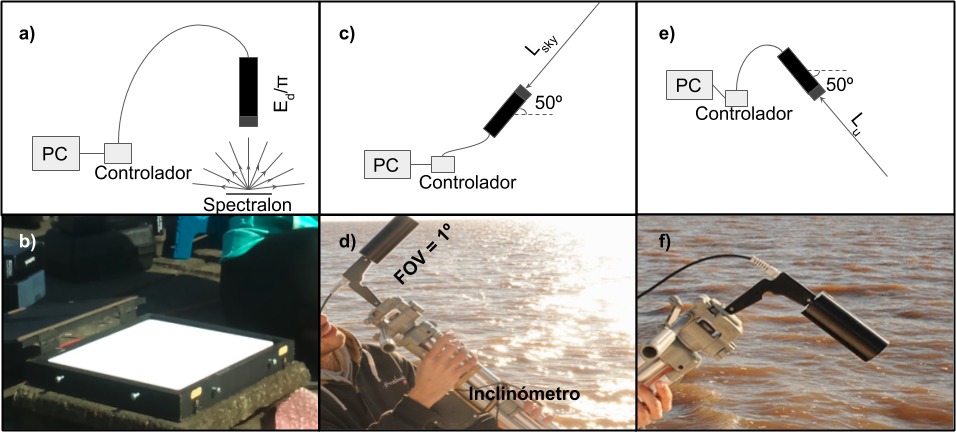
\includegraphics[width=\textwidth]{dat/figures/ASD.png}
    \caption[Disposición del radiómetro ASD utilizada para las mediciones.]{Disposición del radiómetro ASD utilizada para las mediciones. La geometría de sensado se regula mediante un trípode y un inclinómetro. Esquemas de la adquisicón de la irradiancia descendente, $E_{d}$ (a), radiancia ascendente, $L_{u}$ (c) y radiancia del cielo en ángulo horizontal recíproco a $L_{u}$, $L_{sky}$ (e). b),d),f): Fotografías correspondientes a cada una de estas geometrías, campaña RdP\_20140617.}
    \label{dat:ASD}
    \end{figure}

    \subsection{Radiómetro ASD}
    \label{dat:s:asd}
    
        El ASD es un radiómetro hiperespectral de campo en el rango 350-2500 nm cuya geometría de adquisición es regulada por una fibra óptica. El ASD utilizado para llevar a cabo las mediciones que conforman parte de nuestra base de datos pertenece a la CONAE (Comisión Nacional de Actividades Espaciales).

        \subsubsection{ASD: Protocolo de medición}
        \label{dat:s:asdMed}

            La metodología de medición se basa en los protocolos desarrollados y recomendados por la NASA (Mueller et al., 2000 \cite{mueller2003}). Se utilizó una lente con un ángulo de observación (\textit{Field of View} - FOV) de $1 \degree$, la configuración geométrica se describe en la Figura \ref{dat:ASD}, el Cuadro \ref{dat:tab:radiometria} y la configuración del equipo es detallada Dogliotti et al. 2014 \cite{dogliotti2014}.

            Se realizan tres series de mediciones sucesivas en la siguiente secuencia: $E_{d}$, $L_{u}$, $L_{sky}$, $L_{u}$, $L_{sky}$, $L_{u}$, $L_{sky}$, totalizando 21 mediciones (Cuadro \ref{dat:tab:asd}). En cada una de estas será necesario establecer un tiempo de integración del sensor.
            \begin{table}
            \caption{Orden consecutivo de las mediciones realizadas por el espectrorradiómetro ASD durante cada estación.}
                \begin{tabular}{|l|l|l|l|l|l|l|l|}
                \hline
                 & $E_{d}$ & $L_{u}$ & $L_{sky}$ & $L_{u}$ & $L_{sky}$ & $L_{u}$ & $L_{sky}$ \\ \hline
                1$^{ra}$ Serie & 1 & 2 & 3 & 4 & 5 & 6 & 7 \\ \hline
                2$^{da}$ Serie & 8 & 9 & 10 & 11 & 12 & 13 & 14 \\ \hline
                3$^{ra}$ Serie & 15 & 16 & 17 & 18 & 19 & 20 & 21 \\ \hline
                \end{tabular}
            \label{dat:tab:asd}
            \end{table}

        \subsubsection{ASD: Protocolo de procesamiento}
        \label{dat:s:asdProc}
        
            El cálculo de la reflectancia del agua se obtiene de promediar los 9 escaneos - resultantes de los tres escaneos de $L_{u}$ y $L_{sky}$ para cada una de las tres series - obtenidos para la reflectancia (Ec. \ref{dat:eq:rhoWField}), aunque previamente se consideran una serie de criterios para garantizar la obtención de buenas mediciones (estabilidad de $E_{d}$, detección de anomalías y control del desvío estándar en las reflectancias) sobre 4 longitudes de onda en el rango VIS-NIR: $\lambda_{0}$ = 450 nm, 600 nm, 750 nm y 900 nm. Estas longitudes de onda,  distribuidas cada 150 nm, fueron elegidas para que cubran todo el rango de interés y haya solapamiento con las longitudes de onda utilizadas en el protocolo utilizado previamente ($750$ y $900\sim930$ nm). El código de procesamiento fue hecho para que la elección de estas longitudes de onda y los umbrales de los respectivos criterios puedan tomarse como entradas fáciles de modificar. La Figura \ref{dat:ASD_QC} muestra cómo se aplicaron dichos criterios a los escaneos de la estación RdP\_20131220\_DCAO-E.
            
            A continuación se enumeran y describen los criterios de calidad mencionados:

            \begin{enumerate}
                \item \textbf{Criterio de estabilidad de $E_{d}$}: Se asume que si se detectó una alta varibilidad entre las tres mediciones de $E_{d}$ es porque el cielo se hallaba en condiciones de nubosidad variable; por lo que si:
                \begin{equation}
                    max\{E_{d}(\lambda_{0})\} - min\{E_{d}(\lambda_{0})\} > 0.03
                \end{equation}
                
                \noindent
                en alguna de las 4 longitudes de onda mencionadas, se consideran únicamente los escaneos asociados al espectro de $E_{d}$ más alto.

                \item \textbf{Detección de espectros anómalos}: La reflectancia resultante de la serie de mediciones se computa tomando la media espectral. Dado que la media es un estadístico fuertemente sensible a anomalías es fundamental no considerar escaneos anómalos en dicho cómputo. Para ello, se calculan los terciles del conjunto de reflectancias en cada una de las longitudes de onda consideradas y se establece un criterio de detección de valores anómalos a partir del rango intertercil (ITR). Se escogieron terciles y no cuartiles (como es usual) dado que para cada estación el número total de mediciones es 9, por lo que los terciles dividen a las mediciones en tres conjuntos de tres mediciones: La condición que se establece es que si
                
                \begin{equation}
                \begin{aligned}
                \rho_{w}(\lambda_{0},escaneo_{i}) &> T2 + 2.5max\{ITR(\lambda_{0}),0.001\}\\
                \rho_{w}(\lambda_{0},escaneo_{i}) &< T1 - 2.5max\{ITR(\lambda_{0}),0.001\}
                \end{aligned}    
                \label{dat:eq:ITR}
                \end{equation}
                
                \noindent
                entonces se desecha el escaneo. Obsérvese que se considera un valor mínimo de ITR determinado a partir de un umbral de 0.001 para evitar considerar espectros supuestamente anómalos producto de que la variabilidad en la medición resulte demasiado chica en comparación al ruido típico del sensor.

                \item \textbf{Control del desvío estándar}: Una vez aplicados estos criterios, se evalúa el desvío estandar en cada una de las longitudes de onda consideradas, de forma tal de que si
                
                \begin{equation}
                    \sigma(\rho_{w}(\lambda_{0})) > 0.01
                    \label{dat:eq:}
                \end{equation}
                
                \noindent
                en alguna de las 4 longitudes de onda mencionadas, se considera que la medición sigue presentando demasiada variabilidad intrínseca a pesar de los controles de calidad previos; por lo que la misma se descarta.

            \end{enumerate}

            \begin{figure}
            \centering
            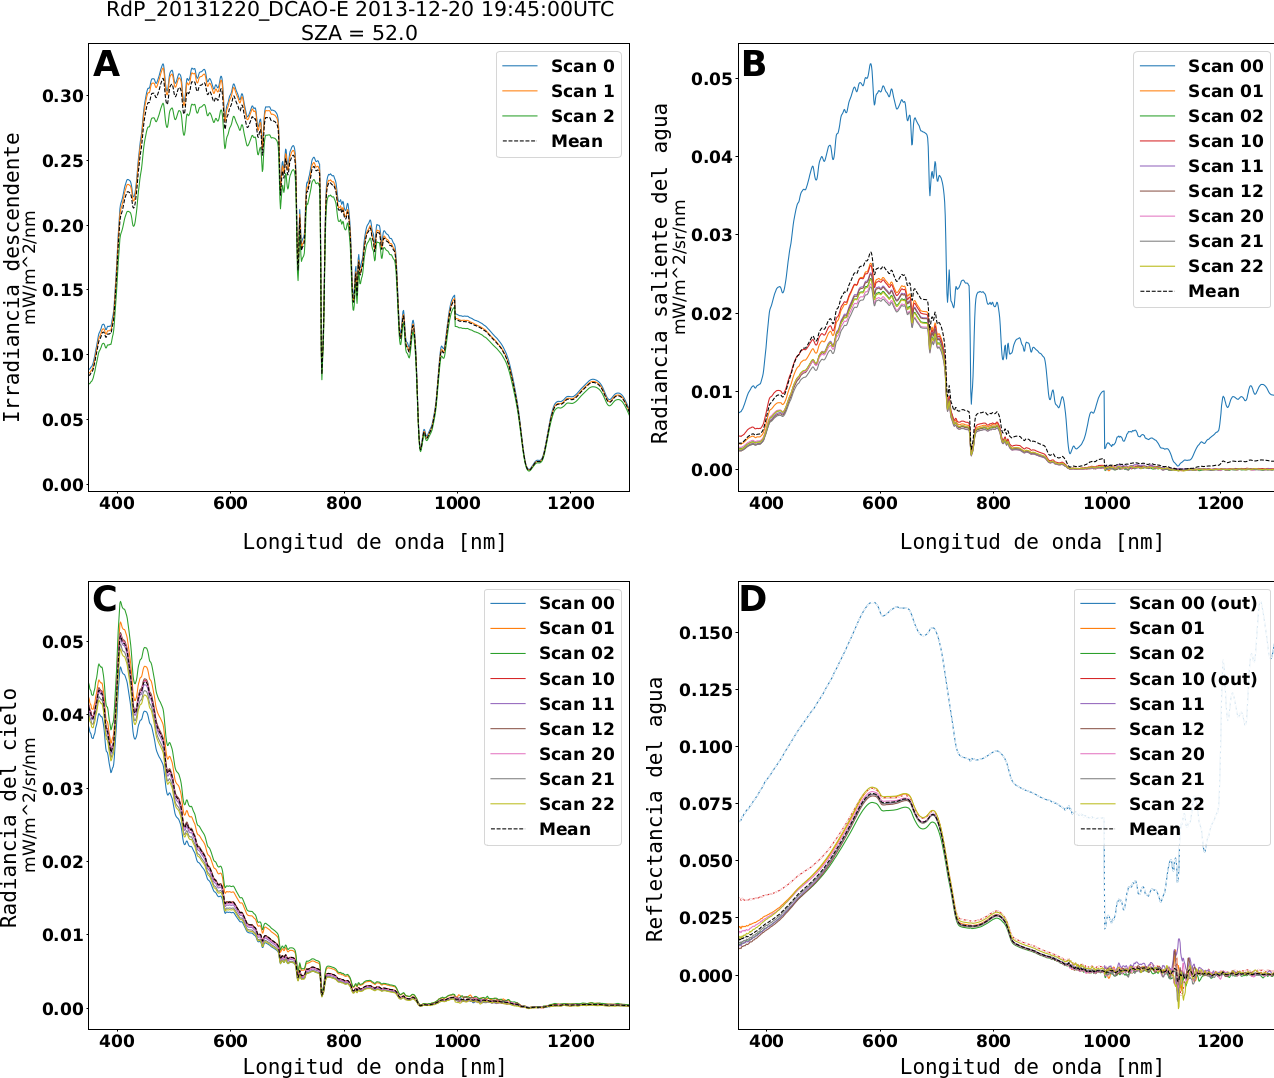
\includegraphics[width=\textwidth]{dat/figures/ASD_QC.png}
            \caption[Control de calidad de los escaneos hechos con el ASD para la estación RdP\_20131220\_DCAO-E.]{Control de calidad de los escaneos hechos con el ASD para la estación RdP\_20131220\_DCAO-E. a) Escaneos de irradiancia descendente, $E_{d}$. b) Escaneos de radiancia ascendente, $L_{u}$. c) Escaneos de radiancia del cielo, $L_{sky}$. d) Reflectancia del agua, $\rho_{w}$, para cada una de las nueve series. Obsérvese que la media computada no tiene en cuenta los espectros anómalos 00 (proveniente de una mala medición de $L_{u}$) y 10 (subestimación de la componente especular del cielo).} 
            \label{dat:ASD_QC}
            \end{figure}


    \subsection{Sistema radiométrico TriOS}
    \label{dat:s:trios}
        
        El radiómetro TriOS mide la luz reflejada en la región visible/infrarrojo cercano (VNIR, $350-950$ nm). A pesar de no medir en el rango del SWIR (en que sí mide el ASD), tiene la ventaja de que mide en simúltaneo los tres espectros requeridos ($E_{d}$, $L_{u}$ y $L_{sky}$), dado que el equipo consta de dos radiómetros y un irradiómetro. Esto lo hace mucho más fácil de operar, y una vez colocado en un soporte mecánico, será mucho más fácil garantizar el correcto posicionamiento de los sensores que en el caso de ASD.

        \subsubsection{TriOS: Protocolo de medición}
        \label{dat:s:triosMed}

            \begin{figure}
            \centering
            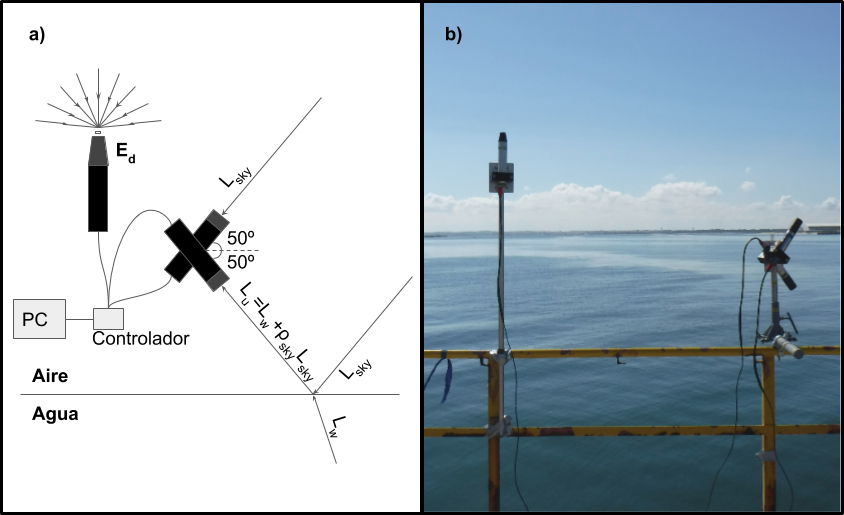
\includegraphics[width=\textwidth]{dat/figures/TriOS.png}
            \caption[Disposición del radiómetro TriOS utilizada para las mediciones.]{Disposición del radiómetro TriOS utilizada para las mediciones. Los tres sensores se manipulan desde el mismo controlador, lo que garantiza simultaneidad de los escaneos. a) Esquema de la geometría (cenital) indicada para los radiómetros ($L_{u}$ y $L_{sky}$) y el irradiómetro ($E_{d}$). b) Fotografía del sistema TriOS colocado sobre el Muelle de Barreiro, en la costa del Estuario del Río Tajo, en Lisboa, Portugal (campaña Tagus\_20190617).}
            \label{dat:TriOS}
            \end{figure}

            El protocolo de medición de TriOS es mucho más sencillo que el del ASD, dado que las mediciones son controladas por un \textit{software} (MSDA\_XE) que automáticamente computa los tiempos de integración y envía las órdenes a los tres sensores para que ejecuten las mediciones en dichos tiempos. Una vez que se quiere realizar la medición, se acciona un disparador global, el cual se mantendrá activo durante aproximadamente 15 minutos. Se fijó esta ventana temporal ya que es lo suficientemente grande como para abarcar una cantidad adecuada de mediciones que superen los estándares de calidad y suficientemente chica como para evitar efectos de varibilidad natural sobre la medición final reportada.
    
        \subsubsection{TriOS: Protocolo de procesamiento}
        \label{dat:s:triosProc}
            
            Los criterios de control de los escaneos se enumeran a continuación:

            \begin{enumerate}
                \item \textbf{Sincronicidad de escaneos}: Seleccionamos previamente los escaneos $E_{d}$, $L_{u}$ y $L_{sky}$ que se sincronizan mutuamente (por ejemplo, eliminamos los escaneos $E_{d}$ que no son simultáneos con ninguno de los de $L_{sky}$ o $L_{u}$). Esto puede suceder cuando los tiempos de integración de los sensores (optimizados automáticamente por TriOS) difieren entre sí. Esto podría ser causado, por ej., por una sombra incidental en cualquiera de los sensores durante las mediciones.

                \item \textbf{Anomalías espectrales}: Descartamos los escaneos que presentan saltos discontinuos (no físicos) en rangos espectrales muy cortos. Hacemos esto comparando valores medidos por el TriOS en longitudes de onda consecutivas. Más precisamente, el escaneo pasa dicho control de calidad si todas las magnitudes $M$ (siendo $E_{d}$, $L_{sky}$ o $L_{sea}$) satisface:
            
                \begin{equation}
                \begin{aligned}
                    M[t_{0}; \lambda + 2.5] - M[t_{0}; \lambda] & <  \alpha[M]*(M[t_{0}; \lambda + 2.5] + M[t_{0}; \lambda])/2\\
                    \alpha[M = E_{d}  ] & = 0.4\\
                    \alpha[M = L_{se} ] & = 2.0\\
                    \alpha[M = L_{sky}] & = 0.4                      
                \end{aligned}
                \end{equation}
                
                Esto se verifica para todos los tiempos de exploración $t_{0}$ y debe cumplirse para todas las longitudes de onda en $[400-947.5]$ nm.

                \item \textbf{Anomalías temporales}: Descartamos los escaneos que presentan picos temporales repentinos. Hacemos esto comparando cada escaneo a tiempo $t=t_{0}$ con el escaneo anterior/posterior, a $t_{0}\pm dt$ a la longitud de onda particular de $550$ nm. Más precisamente, el escaneo deberá satisfacer:

                \begin{equation}
                \begin{aligned}
                    M[t_{0} \pm dt; 550] - M[t_{0}; 550] & <  \beta[M]*(M[t_{0} \pm dt; 550] + M[t_{0}; 550])/2\\
                    \beta[M = Ed  ] & = 0.25\\
                    \beta[M = Lse ] & = 0.25\\
                    \beta[M = Lsky] & = 0.25\\
                \end{aligned}
                \end{equation}
            
                \item \textbf{Desvío de $E_{d}$ del cenit}: Descartamos aquellos escaneos donde el ángulo comprendido entre la medición de $E_{d}$ y el cenit (medido con un inclinómetro adosado al irradiómetro) es mayor a $5 \degree$.
            
                \item \textbf{Selección de escaneos y cómputo de estadísticos}: Una vez que todos estos criterios son considerados, seleccionamos los primeros 5 escaneos válidos (i.e. que hayan pasado todos los controles anteriores). Para este conjunto de escaneos se computan la media ($\mu$), el desvío estándar ($\sigma$) y el coeficiente de variación ($CV = 100\times\sigma/\mu$).

                La Figura \ref{dat:TriOS_QC} muestra cómo dichos criterios fueron aplicados a los escaneos de la estación RdP\_20181202\_ST05.
            
                \begin{figure}
                \centering
                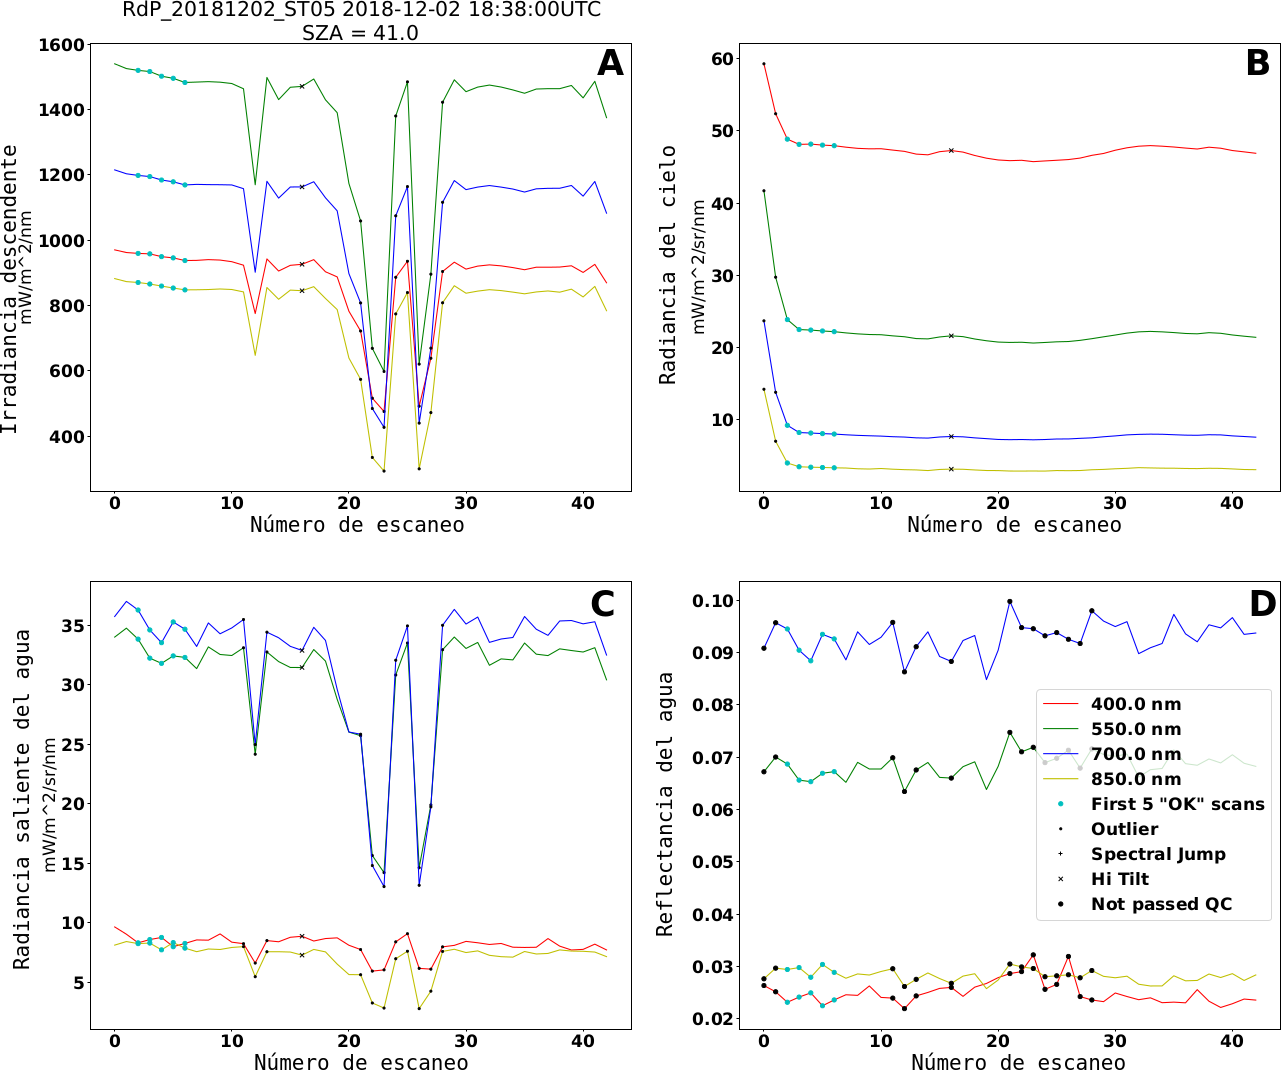
\includegraphics[width=\textwidth]{dat/figures/TriOS_QC.png}
                \caption[Control de calidad de los escaneos hechos con el TriOS para la estación RdP\_20181202\_ST05.]{Control de calidad de los escaneos hechos con el TriOS para la estación RdP\_20181202\_ST05. Escaneos a 400 nm, 550 nm, 700 nm y 850 nm de irradiancia descendente, $E_{d}$ (a), radiancia ascendente, $L_{u}$ (b), radiancia del cielo, $L_{sky}$ (c) y reflectancia del agua, $\rho_{w}$ (d). Todos los criterios de calidad mencionados previamente (anomalías temorales, espectrales y de ángulo cenital elevado) son evaluados previo a seleccionar los primeros cinco escaneos de calidad (señalados en cian).} 
                \label{dat:TriOS_QC}
                \end{figure}
                
                
                \item \textbf{Condiciones de baja variabilidad}: La siguiente condición debe ser satisfecha para asegurar una variabilidad aceptablemente baja entre los 5 escaneos seleccionados:
                
                \begin{equation}
                    std(\rho_{w}(750)) < 0.05
                \end{equation}
            \end{enumerate}
            
\section{Mediciones de turbidez}
\label{dat:s:turbidez}

    La \textit{turbidez} puede ser definida cualitativamente como la reducción de la transparencia de un líquido causada por la presencia de materia no disuelta.
    En términos ópticos, y siguiendo el estándar definido por la norma ISO 7027, la turbidez de una muestra de fluido (en nuestro caso, aguas naturales) se establece determinando qué fracción de luz - proveniente de un LED en el inrarrojo cercano - es dispersada a $90\degree$ por una muestra dada. A su vez, se puede refinar la medición determinando en simultáneo la fracción transmitida del haz incidente. Un instrumento que mide la turbidez únicamente a partir de la dispersión a $90\degree$ se denomina \textit{nefelómetro}; mientras que si se vale a su vez de la detección de la fracción de radiación transmitida el instrumento se denomina \textit{turbidímetro}. Los fotones capturados por el/los fotodiodo/s se transforman en una corriente eléctrica que es trasducida a unidades de turbidez. Si el nefelómetro o turbidímetro es calibrado según los estándares de la ISO 7027, las unidades utilizadas se llaman FNU (Formazin Nephelometric Units). Estas unidades se refieren a una sustancia patrón llamada formazina y se convierten idénticamente a la concentración de dicha sustancia en \textit{mg/l}. Es decir que se trasduce al valor de \textit{x FNU} al voltaje medido por el nefelómetro/turbidímetro sobre una muestra de formazina (en agua pura) de concentración \textit{x mg/l}.
    
    Existen diversas unidades de medición de turbidez según la sustancia patrón utilizada, la fuente emisora y la geometría de detección de los fotodiodos del sensor. En este capítulo utilizaremos dos unidades, ambas determinadas a partir de la formazina: las FNU (ya descritas) y las FBU (\textit{Formazin Backscatter Units}). Tal como su nombre lo indica, estas útlimas corresponden a la trasducción voltaje-concentración de formazina, pero utilizando un retrodispersómetro en vez de un nefelómetro. Es fundamental notar que, for definición, dichas unidades son equivalentes \textit{para una muestra de formazina}, es decir, \textit{1 FNU = 1 FBU = 1 mg/l} de formazina. Sin embargo, dicha identidad no es válida en el caso general, sino que la relación entre estas unidades será dependiente de la geometría de la función de dispersión volumétrica (\textit{Volume Scattering Function}, VSF o $\beta$, Ec. \ref{qssa:eq:vsf}) de la muestra considerada.
    
    Hay un gran interés de los usuarios en monitorear la turbidez de las aguas costeras y estuarinas (Dogliotti et al. 2015, \cite{dogliotti2015}). El mapeo satelital de la turbidez es relevante tanto como un indicador del entorno óptico para fines de monitoreo de la calidad del agua (Nechad et al. 2009, \cite{nechad2010}) como por ser un \textit{proxy} fácilmente medible de la concentración de partículas suspendidas (SPM) en aplicaciones de transporte de sedimentos (Gippel 1995, \cite{gippel1995}). Con respecto al monitoreo de la calidad del agua, la turbidez es considerada un parámetro obligatorio que deben medir los estados miembros de la Unión Europea en la Directiva Marco de la Estrategia Marina (Unión Europea, 2008, \cite{eu2008}).

    \subsection{Turbidímetro portátil \textit{HACH 2100Q is}}
    \label{dat:s:hach}

        El \textit{HACH 2100Q is} es un turbidímetro portátil que satisface el estándar de la ISO 7027. Este instrumento determina la turbidez mediante la razón de la radiación dispersiada a $90 \degree$ y la transmisitida, proveniente de un LED a 860 nm (Figura \ref{dat:HACH}). El instrumento mide turbidez entre 0 y 999 FNU con una resolución de tres dígitos y fue programado para promediar una serie de 12 escaneos sucesivos para minimizar el impacto del ruido.
        
        \begin{figure}
        \centering
        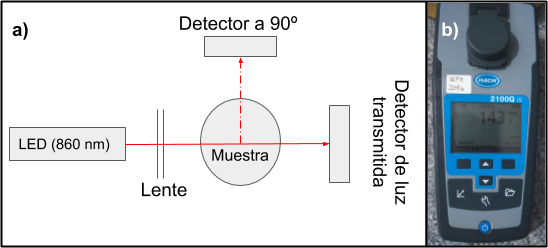
\includegraphics[width=0.8\textwidth]{dat/figures/HACH.png}
        \caption[Esquema y fotografía del turbidímetro portátil \textit{HACH 2100Q is} (ISO 7027).]{Turbidímetro portátil \textit{HACH 2100Q is} (ISO 7027). a) Esquema del funcionamiento del turbidímetro. b) Fotografía de uno de los turbidímetros utilizados en nuestro grupo (IAFE 2016), reportando un valor de 143 FNU (tras haber promediado 12 escaneos).}
        \label{dat:HACH}
        \end{figure}

        \subsubsection{HACH: Protocolo de medición}
        \label{dat:s:hachMed}

            Para realizar las mediciones se utiliza la siguiente metodología:
            \begin{itemize}
                \item Chequear la estabilidad del instrumento usando los estándares de formazina.
                \item Enjuagar y llenar el vial de vidrio con la muestra (10 ml).
                \item Enjuagar el lado exterior del vial con agua ultra pura (milliQ).
                \item Secar el exterior con papel de pulpa de celulosa (tisú).
                \item Ungir la cara exterior del vial con gel de silicona para homogeneizar el índice de refracción del vial en caso de que el vidrio presentase microgrietas de vidrio.
                \item Voltear suavemente la muestra para homogeneizarla. Evitar la formación de burbujas y gotas de condensación que pudieren alterar la medición.
                \item Realizar la medición de turbidez con el HACH 3 veces repitiendo el paso anterior entre cada repetición.
            \end{itemize}
            A partir de estas tres mediciones se obtendrán el valor medio y el desvío estándar y se asociarán al valor reportado con su error, respectivamente.

        \subsubsection{HACH: Protocolo de procesamiento}
        \label{dat:s:hachProc}
        
            El único control de calidad que se hace sobre las mediciones una vez realizadas es chequear que el coeficiente de variación no supere el 20 \%. En caso de superarse, se descarta la medición más alejada de la mediana. De todas formas, esta situación es extremadamente rara - de hecho, jamás se nos presentó - dado que el turbidímetro HACH provee mediciones muy estables que suelen tener coeficientes de variación menores al 5\%.
    
    \subsection{Medidores de turbidez en continuo \textit{OBS501}}
    \label{dat:s:obs}
    
    % , por lo que los llamaremos turbidímetros al igual que el HACH, aunque no satisfacen propiamente la definición planteada en la \S \ref{dat:s:turbidez}
        El sensor OBS501 es una combinación de dos dispersómetros (calibrados en unidades de turbidez) de medición continua que, al contrario del HACH, mide estando sumergido en el agua (Figura \ref{dat:OBS}). Ambos medidores de turbidez sensan la luz emitida por un láser VCCS (Voltage-Controlled Current Source) a 850 nm: uno de ellos es un nefelómetro (ISO 7027) y el otro un \textit{retrodispersómetro}. Ambos fueron calibrados con formazina, por lo que el nefelómetro provee valores de turbidez en FNU (magnitud llamada aquí T\_OBS501\_SS, por \textit{side-scattering}), mientras que el retrodispersómetro provee valores en FBU (magnitud llamada aquí T\_OBS501\_BS, por \textit{back-scattering}). Es importante notar que, a diferencia del HACH, el OBS carece de transmisómetro.
        
        \begin{figure}
        \centering
        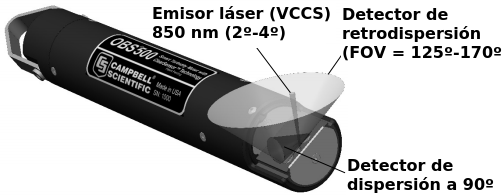
\includegraphics[width=0.8\textwidth]{dat/figures/OBS.png}
        \caption[Fotografía del OBS mostrando los conos de emisión del láser y sensado del nefelómetro y el retrodispersómetro.]{Fotografía del OBS mostrando los conos de emisión del láser y sensado del nefelómetro (T\_OBS501\_SS) y el retrodispersómetro (T\_OBS501\_BS).}
        \label{dat:OBS}
        \end{figure}

        \subsubsection{OBS: Protocolo de medición}
        \label{dat:s:obsMed}

            El OBS501 mide sumergido en el cuerpo de agua, aunque su autonomía es limitada, dado que debe ser comandado desde la superficie por un controlador (o \textit{datalogger}) no sumergible, el \textit{CR-800}. El CR-800 envía diversos comandos  - escaneo, encendido, apagado y activación del limpia-ópticas - al OBS 501 establecidos en un programa escrito en \textit{CRBasic}. En nuestro caso, se diseñó un programa que permitió ejecutar el siguiente protocolo: durante cada jornada de medición, el OBS501 se dispuso a medir cada 5 segundos durante un período continuo que abarcó desde la primera hasta la última de las estaciones de la jornada en determinado sitio.% Luego, se establecieron una serie de criterios para determinar el valor e incerteza de cada estación, detallados en la próxima sección.
            
        
        \subsubsection{OBS: Protocolo de procesamiento}
        \label{dat:s:obsProc}
        
            Para cada campaña se obtienen los valores en continuo de todas los datos de turbidez en FNU (T\_OBS501\_SS) y FBU (T\_OBS501\_BS), entre otras variables misceláneas. Estos datos se almacenan según tres criterios temporales: los datos en crudo, los datos suavizados a 1 minuto y los datos por estación.
            
            Tanto para los datos suavizados como para los datos por estación se selecciona una ventana temporal de los datos crudos: en el primer caso, una ventana móvil de 1 minuto y en el segundo, una ventana de 5 minutos centrada en el horario oficial de la estación (determinado generalmente por la medición radiométrica). En ambos casos, se eliminan escaneos anómalos dentro de dicha ventana, apelando al criterio del rango intercuartil (\textit{Inter-Quartile Range}, IQR, similar a Ec. \ref{dat:eq:ITR}), es decir, \textit{x} es un escaneo anómalo si:
            
            \begin{equation}
                \begin{aligned}
                x &> Q3 + 1.5 IQR\\
                x &< Q1 - 1.5 IQR
                \end{aligned}    
                \label{dat:eq:IQR}
            \end{equation}

            \noindent 
            siendo \textit{Q1} y \textit{Q3} los primer y tercer cuartiles. Una vez eliminados los valores anómalos, se computan la mediana y el desvío estándar dentro de la ventana y se asocian al valor reportado y a la incerteza, respectivamente. Si el coeficiente de variación supera el 15\%, el valor de la ventana no es considerado de buena calidad.

    \subsection{Validación del algoritmo de turbidez de Dogliotti et al. 2015}
    \label{dat:s:dog15}

        A su vez, para intercomparar las mediciones de turbidez con las radiométricas se computó y testeó el algoritmo de turbidez propuesto por Dogliotti et al. 2015, \cite{dogliotti2015} a partir de las reflectancias del agua medidas:

        \begin{equation}
        \begin{aligned}
            T(\lambda) & = \frac{A(\lambda).\rho_{w}(\lambda)}{1-\rho_{w}(\lambda)/C(\lambda)}, \quad\quad \lambda = 645\,nm,\,860\,nm\\
            \omega & = max\{min\{(\rho_{w}(645)-0.05)/0.02;1\};0\}\\
            T\_Dogliotti & = T(645).(1-\omega) + T(860).\omega
        \end{aligned}
        \label{dat:eq:dogliotti2015}
        \end{equation}

        \noindent siendo $A(645) = 228.1$ FNU, $A(860) = 3078.9$ FNU, $C(645) = 0.1641$ y $C(860) = 0.2112$.

\section{Mediciones de Material Particulado en Suspensión}
\label{dat:s:spm}

    La concentración de material particulado total en suspensión (\textit{Suspended Particulate Matter}, SPM) es la razón entre la masa neta del material colectado en un filtro GF/F por filtración y el correspondiente volumen de agua filtrado. Es una concentración masa en volumen y sus unidades usuales son $mg/l$. El método utilizado se denomina \textit{gravimétrico} y está descripto en Tilstone et al. 2003, \cite{tilstone2003} y basado en van der Linde 1998, \cite{vanderlinde1998}.
    
    \subsection{SPM: Protocolo de medición}
    \label{dat:s:spmMed}

        Las muestras de superficie son filtradas en filtros GF/F pre-combustionados y pre-pesados y luego de filtrar la muestra (Figura \ref{dat:SPM}), los mismos son secados y vueltos a pesar, para obtener así el peso por unidad de volumen filtrado. La concentración del material particulado inorgánico (SIM, \textit{Suspended Inorganic Matter}) se calcula mediante el combustionado posterior de los filtros, para eliminar los compuestos orgánicos, y repesado de los mismos. Finalmente la concentración del material particulado orgánico (SOM, \textit{Suspended Organic Matter}) se estima a partir de la diferencia entre el inorgánico y el total. La metodología es descrita a continuación:
        
        \begin{itemize}
            \item Preparación de los filtros
            \begin{itemize}
                \item Pre-combustión de los filtros a 450$\degree$C por 1 hora y lavado con agua milliQ.
                \item Secado de los filtros a 75$\degree$ C por 1 hora y almacenamiento en gel de silicona.
            \end{itemize}
            \item Determinación de SPM
                \begin{itemize}
                    \item Pesaje de los filtros secos (pesaje \textit{M0}).
                    \item Filtrado de un volumen de muestra (\textit{V}) a presiones de succión de $300-400 mmHg$.
                    \item Secado de los filtros en estufa a 75$\degree$C por 24 horas.
                    \item Pesaje de los filtros en la misma balanza usada previamente (pesaje \textit{M1}).
                    \item Determinación de SPM a partir de:
                        \begin{equation}
                            SPM = (M1-M0)/V
                            \label{dat:eq:SPM}
                        \end{equation}
                \end{itemize}
            \item Determinación de SIM y SOM
                \begin{itemize}
                    \item Combustionado de los filtros a 450$\degree$C por 5 horas (ó 4 horas a 550$\degree$C)
                    \item Pesaje de los filtros en la misma balanza usada previamente (pesaje \textit{M2})
                \end{itemize}
                \item Determinación de SIM y SOM a partir de:
                \begin{align}
                    SIM & = (M2-M0)/V\\
                    SOM & = SPM-SIM
                \end{align}
        \end{itemize}

        \begin{figure}
            \centering
            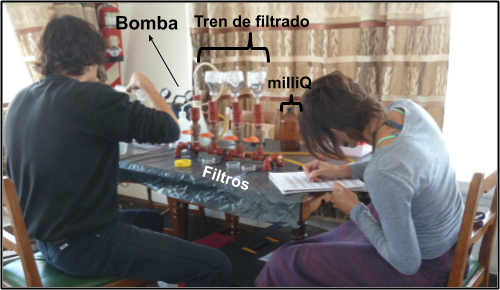
\includegraphics[width=0.75\textwidth]{dat/figures/SPM.png}
            \caption[Fotografía del tren de filtrado utilizado para obtener las mediciones de material particulado total, inorgánico y orgánico.]{Fotografía del tren de filtrado generalmente utilizado para obtener las mediciones de material particulado total (SPM), inorgánico (SIM) y orgánico (SOM).}
            \label{dat:SPM}
        \end{figure}
            
    \subsection{SPM: Protocolo de procesamiento}
    \label{dat:s:spmProc}
    
        Las mediciones por estación suelen hacerse por triplicado (de lo contrario se utiliza un único filtro). En dicho caso, se toma como valor reportado e incerteza a la media y desvío estándar y se descarta la medición si el coeficiente de variación supera el 20\%. 

    \subsection{Validación del algoritmo de SPM de Nechad et al. 2010}
    \label{dat:s:spmNech10}

        Por último, para comparar las mediciones de SPM con las radiométricas se computó y testeó el algoritmo de SPM propuesto por Nechad et al. 2010, \cite{nechad2010}, a partir de las reflectancias del agua medidas:

        \begin{equation}
            SPM\_Nechad = \frac{A(645).\rho_{w}(645)}{1-\rho_{w}(645)/C(645)} + B(645)
            \label{dat:eq:nechad2010}
        \end{equation}

        \noindent
        siendo $A(645) = 253.51 mg/l$, $B(645) = 2.32 mg/l$ y $C(645) = 0.1641$.
        
        
\section{Estructura de la base de datos}
\label{dat:s:basedatos}
    La base de datos presentada en este capítulo se creó siguiendo la lógica estándar de organización de la información usada en lenguajes de consulta de datos (DQLs, \textit{data query languages}, ver Cuadro \ref{dat:tab:metadata}). Es decir, los datos se estructuran en tablas bidimensionales en que cada columna se corresponde con un campo (por ejemplo, la latitud) y cada nueva fila una nueva entrada a la base de datos - una estación. A su vez, cada entrada/estación posee un código único identificatorio llamado \textit{llave} (\textit{key} en DQLs) que permite concatenar con sencillez los campos correspondientes a distintas tablas, y que debe figurar en todas ellas. A modo de ejemplo, supongamos que queremos comparar los datos de turbidez y los de SPM, cuyos campos se hallan en distintas tablas. El hecho de que en ambas figure el campo llave nos permite concatenarlas evitando errores que puedan surgir de la ausencia de entrada para alguna estación en alguno de los campos requeridos. 
    
    \subsection{Sistematización de las diferentes entradas}
    \label{dat:s:entradas}

        Los datos iniciales que conforman la base de datos no estaban originalmente estructurados siguiendo la lógica DQL, por lo que fue necesario reorganizarlos para poder generar un formato común de almacenamiento. De esta forma, se estructuraron las entradas (estaciones) de la base según a qué región pertenecían y según la campaña en la que fueron realizadas. Para cada región se asignó una sigla o acrónimo (e.g. \textit{RdP} para el Río de la Plata, \textit{BALakes} para las lagunas de la Provincia de Buenos Aires) y para nombrar a cada campaña se yuxtapuso a dicha sigla la fecha de la jornada inicial en formato $aaaammdd$ (año-mes-día). Por ejemplo, el Cuadro \ref{dat:tab:metadata} corresponde a la campaña $RdP\_20180404$, es decir, realizada en algún sitio del RdP a partir del 4 de abril de 2018.
        
        Para cada campaña se generó un subdirectorio dentro del directorio de la región correspondiente donde se archivaron las entradas en varias hojas de formato Excel, cada cual conteniendo un conjunto determinado de campos. Por ejemplo, el Cuadro \ref{dat:tab:metadata} corresponde a la hoja de Excel \textit{StationInfo}, donde se guardan los campos de la informacion general de las estaciones: horario de inicio y finalización, fecha, día, latitud, longitud, pasadas satelitales, etc.
                    
    \subsection{Código indentificatorio único de cada estación}
    \label{dat:s:codigo}
     
        Originalmente, la base de datos no poseía un campo al que se le pudiera asignar el rol de llave o código identificatorio. Si bien, dentro de cada campaña, cada estación se nombró de manera unívoca, entre campañas existían entradas de llave repetida que no necesariamente correspondían a la misma ubicación geográfica ni fecha. Para solventar esto se yuxtapuso del nombre de la campaña al nombre de la estación para generar la llave. Por ejemplo, la llave \textit{RdP\_20130430\_PP02-04} corresponde unívocamente a la estación PP02-04 de la campaña realizada a partir del 30 de abril del 2013 en la región del RdP.
        
        La razón por la que se dividieron los datos a partir de las distintas regiones y campañas y los distintos campos en planillas Excel y no en un gran archivo que contuviera a todos los datos fue fundamentalmente la de facilitar la visualización e interpretación de los mismos por los usuarios y garantizar la estabilidad del \textit{software} utilizado para hacer las consultas a la base. Dicho \textit{software} es el módulo \textit{pandas} (Python Data Analysis Library) del lenguaje de programación \textit{Python}. Aparte, los datos recopilados previo al inicio de la construcción de la base fueron históricamente jerarquizados según región y campaña, por lo que se prefirió sostener la jerarquización preexistente.
    
        \begin{table}
        \tiny
        \caption{Información general de las estaciones correspondientes a la campaña RdP\_20180404}
        \begin{adjustbox}{angle=90}
        \begin{tabularx}{1.4\textwidth}{|l|l|l|X|X|X|X|X|X|X|X|X|}
        \hline
        \rowcolor[HTML]{FFFC9E} 
        \textbf{Station ID} & \textbf{Region} & \textbf{Subregion} & \textbf{Pontoon/Vessel/Place} & \textbf{Lat} & \textbf{Lon} & \textbf{Date UTC} & \textbf{start Time UTC} & \textbf{end Time UTC} & \textbf{time Stamp UTC} & \textbf{Overpasses} \\ \hline
        P01 & RdP & CABA & Palermo (Pier) & -34.560754 & -58.39881 & 04/04/18 & 13:36 & 13:46 & 04/04/2018 13:36:00 &  \\ \hline
        P02 & RdP & CABA & Palermo (Pier) & -34.560754 & -58.39881 & 04/04/18 & 14:04 & 14:14 & 04/04/2018 14:04:00 & S2B \\ \hline
        P03 & RdP & CABA & Palermo (Pier) & -34.560754 & -58.39881 & 04/04/18 & 14:34 & 14:49 & 04/04/2018 14:34:00 &  \\ \hline
        P04 & RdP & CABA & Palermo (Pier) & -34.560754 & -58.39881 & 04/04/18 & 15:04 & 15:14 & 04/04/2018 15:04:00 &  \\ \hline
        P05 & RdP & CABA & Palermo (Pier) & -34.560754 & -58.39881 & 04/04/18 & 16:04 & 16:16 & 04/04/2018 16:04:00 &  \\ \hline
        P06 & RdP & CABA & Palermo (Pier) & -34.560754 & -58.39881 & 04/04/18 & 17:20 & 17:25 & 04/04/2018 17:20:00 &  \\ \hline
        P07 & RdP & CABA & Palermo (Pier) & -34.560754 & -58.39881 & 04/04/18 & 17:30 & 17:45 & 04/04/2018 17:30:00 & VIIRS \\ \hline
        P08 & RdP & CABA & Palermo (Pier) & -34.560754 & -58.39881 & 04/04/18 & 18:32 & 18:44 & 04/04/2018 18:32:00 &  \\ \hline
        P09 & RdP & CABA & Palermo (Pier) & -34.560754 & -58.39881 & 05/04/18 & 13:00 & 13:10 & 04/05/2018 13:00:00 &  \\ \hline
        P10 & RdP & CABA & Palermo (Pier) & -34.560754 & -58.39881 & 05/04/18 & 13:43 & 14:01 & 04/05/2018 13:43:00 & S3A \\ \hline
        P11 & RdP & CABA & Palermo (Pier) & -34.560754 & -58.39881 & 05/04/18 & 14:35 & 14:49 & 04/05/2018 14:35:00 &  \\ \hline
        P12 & RdP & CABA & Palermo (Pier) & -34.560754 & -58.39881 & 05/04/18 & 15:38 & 15:51 & 04/05/2018 15:38:00 &  \\ \hline
        P13 & RdP & CABA & Palermo (Pier) & -34.560754 & -58.39881 & 05/04/18 & 16:38 & 16:49 & 04/05/2018 16:38:00 &  \\ \hline
        P14 & RdP & CABA & Palermo (Pier) & -34.560754 & -58.39881 & 05/04/18 & 17:16 & 17:29 & 04/05/2018 17:16:00 & VIIRS \\ \hline
        P15 & RdP & CABA & Palermo (Pier) & -34.560754 & -58.39881 & 05/04/18 & 18:01 & 18:17:39 & 04/05/2018 18:01:30 & Aqua \\ \hline
        P16 & RdP & CABA & Palermo (Pier) & -34.560754 & -58.39881 & 05/04/18 & 18:40 & 18:50 & 04/05/2018 18:40:00 &  \\ \hline
        P17 & RdP & CABA & Palermo (Pier) & -34.560754 & -58.39881 & 06/04/18 & 13:33 &  & 04/06/2018 13:33:00 &  \\ \hline
        P18 & RdP & CABA & Palermo (Pier) & -34.560754 & -58.39881 & 06/04/18 & 14:38 &  & 04/06/2018 14:38:00 &  \\ \hline
        P19 & RdP & CABA & Palermo (Pier) & -34.560754 & -58.39881 & 06/04/18 & 15:33 &  & 04/06/2018 15:33:00 &  \\ \hline
        P20 & RdP & CABA & Palermo (Pier) & -34.560754 & -58.39881 & 06/04/18 & 16:38 &  & 04/06/2018 16:38:00 &  \\ \hline
        P21 & RdP & CABA & Palermo (Pier) & -34.560754 & -58.39881 & 06/04/18 & 17:39 &  & 04/06/2018 17:39:00 &  \\ \hline
        P22 & RdP & CABA & Palermo (Pier) & -34.560754 & -58.39881 & 06/04/18 & 18:41 &  & 04/06/2018 18:41:00 &  \\ \hline
        P-B & RdP & CABA & Palermo (Pier) & -34.562928 & -58.402581 & 06/04/18 & 19:00 &  & 04/06/2018 19:00:00 &  \\ \hline
        \end{tabularx}
        \end{adjustbox}
        \label{dat:tab:metadata}
        \end{table}

    \subsection{Sistematización de los diferentes campos}
    \label{dat:s:campos}

        Como ya fue mencionado, los campos se almacenaron en tablas diferentes según el instrumento de medición. A continuación, enumeramos algunos ejemplos:

        \begin{enumerate}
            \item \textbf{Radiometría}. Dado que los datos radiométricos son vectoriales, cada espectro obtenido se traduce en $N$ campos, siendo $N$ el número total de longitudes de onda ($N=241$ en el caso de TriOS, que fue dispuesto para medir en el rango $350:2.5:950$ nm; $N=2151$ en el caso de ASD, que fue dispuesto para medir en el rango $350:1:2500$ nm). Por lo que los productos espectrales finales derivados de la radiometría (reflectancia media y desvío estándar) son almacenados en hojas separadas para garantizar una visualización adecuada. A su vez, los productos intermedios derivados en el cómputo de estos espectros son guardados en planillas auxiliares (e.g. el conjuto total de escaneos, los valores medios de $E_{d}$, $L_{sky}$ y $L_{u}$, etc.). Por último, se guardan en una hoja aparte el coeficiente de Fresnel equivalente, $\rho_{sky}$, el ángulo cenital solar al momento de la adquisición, $SZA [\degree]$, y los campos de los estadísticos de relevancia a ser utilizados en los controles de calidad: $L_{sky}:E_{d}(750)$, $std[\rho_{w}(750)]$, $CV(780) [\%]$,	$CV(860) [\%]$ y $Max\{CV(400:900)\} [\%]$.	
            \item \textbf{Turbidez HACH}. Los datos de turbidez medidos con turbidímetros HACH se almacenaron según muestra el Cuadro \ref{dat:tab:hach}. Para ello fue necesario crear campos compuestos, dado que para cada turbidímetro HACH utilizado se guardan los triplicados, el promedio y el coeficiente de variación. El módulo \textit{pandas} permite identificar campos compuestos al indicarle un número de filas mayor a uno que corresponden a los nombres de los campos. En este caso, las primeras dos filas (en amarillo en el Cuadro \ref{dat:tab:hach} son interpretadas como descriptoras del campo correspondiente. Asimismo, \textit{pandas} almacena los campos compuestos como duplas de caracteres. Por ejemplo, al campo \textit{sample1} del turbidímetro \textit{HACH2016} se le asigna el nombre \textit{('HACH2016','sample1')}.
        \end{enumerate}

        \begin{table}
        \tiny
        \caption{Mediciones de turbidez (HACH) de las estaciones correspondientes a la campaña RdP\_20180404.}
        \begin{adjustbox}{angle=90}
        \begin{tabular}{|l|l|l|l|l|l|l|l|l|l|l|l|l|l|}
        \hline
        \rowcolor[HTML]{FFFC9E} 
        \cellcolor[HTML]{FFFC9E} & \cellcolor[HTML]{FFFC9E} & \cellcolor[HTML]{FFFC9E} & \cellcolor[HTML]{FFFC9E} & \multicolumn{5}{l|}{\cellcolor[HTML]{FFFC9E}\textbf{IAFE2016{[}FNU{]}}} & \multicolumn{5}{l|}{\cellcolor[HTML]{FFFC9E}\textbf{RBINS2009{[}FNU{]}}} \\ \cline{5-14} 
        \rowcolor[HTML]{FFFC9E} 
        \multirow{-2}{*}{\cellcolor[HTML]{FFFC9E}\textbf{\begin{tabular}[c]{@{}l@{}}Station\\ ID\end{tabular}}} & \multirow{-2}{*}{\cellcolor[HTML]{FFFC9E}\textbf{timeStampUTC}} & \multirow{-2}{*}{\cellcolor[HTML]{FFFC9E}\textbf{\begin{tabular}[c]{@{}l@{}}globalMean\\ {[}FNU{]}\end{tabular}}} & \multirow{-2}{*}{\cellcolor[HTML]{FFFC9E}\textbf{\begin{tabular}[c]{@{}l@{}}globalCV\\ {[}\%{]}\end{tabular}}} & \textbf{sample1} & \textbf{sample2} & \textbf{sample3} & \textbf{Mean} & \textbf{CV{[}\%{]}} & \textbf{sample1} & \textbf{sample2} & \textbf{sample3} & \textbf{Mean} & \textbf{CV{[}\%{]}} \\ \hline
        P01 & 04/04/2018 13:38:00 & 107.50 & 2.18 & 108.00 & 106.00 & 104.00 & 106.00 & 1.89 & 108.00 & 108.00 & 111.00 & 109.00 & 1.59 \\ \hline
        P02 & 04/04/2018 14:18:00 & 111.50 & 2.25 & 110.00 & 116.00 & 109.00 & 111.67 & 3.39 & 112.00 & 112.00 & 110.00 & 111.33 & 1.04 \\ \hline
        P03 & 04/04/2018 14:36:00 & 111.33 & 1.77 & 111.00 & 112.00 & 108.00 & 110.33 & 1.89 & 111.00 & 112.00 & 114.00 & 112.33 & 1.36 \\ \hline
        P04 & 04/04/2018 15:09:00 & 102.27 & 2.24 & 98.60 & 101.00 & 102.00 & 100.53 & 1.74 & 105.00 & 104.00 & 103.00 & 104.00 & 0.96 \\ \hline
        P05 & 04/04/2018 16:05:00 & 92.10 & 2.68 & 91.80 & 88.80 & 89.70 & 90.10 & 1.71 & 94.70 & 94.60 & 93.00 & 94.10 & 1.01 \\ \hline
        P06 & 04/04/2018 17:04:00 & 92.07 & 1.69 & 92.40 & 92.00 & 90.60 & 91.67 & 1.03 & 91.70 & 94.90 & 90.80 & 92.47 & 2.33 \\ \hline
        P07 & 04/04/2018 17:34:00 & 97.23 & 1.63 & 96.80 & 97.30 & 96.10 & 96.73 & 0.62 & 95.20 & 99.60 & 98.40 & 97.73 & 2.33 \\ \hline
        P08 & 04/04/2018 18:36:00 & 102.33 & 0.80 & 101.00 & 103.00 & 103.00 & 102.33 & 1.13 & 103.00 & 102.00 & 102.00 & 102.33 & 0.56 \\ \hline
        P09 & 04/05/2018 13:02:00 & 81.32 & 0.78 & 80.90 & 80.60 & 81.00 & 80.83 & 0.26 & 81.20 & 82.10 & 82.10 & 81.80 & 0.64 \\ \hline
        P10 & 04/05/2018 13:50:00 & 78.90 & 1.15 & 78.70 & 77.90 & 78.60 & 78.40 & 0.56 & 80.50 & 79.30 & 78.40 & 79.40 & 1.33 \\ \hline
        P11 & 04/05/2018 14:35:00 & 83.02 & 0.73 & 82.60 & 82.20 & 82.80 & 82.53 & 0.37 & 83.30 & 83.90 & 83.30 & 83.50 & 0.41 \\ \hline
        P12 & 04/05/2018 15:36:00 & 105.83 & 2.02 & 104.00 & 104.00 & 104.00 & 104.00 & 0.00 & 109.00 & 107.00 & 107.00 & 107.67 & 1.07 \\ \hline
        P13 & 04/05/2018 16:36:00 & 91.52 & 1.47 & 90.80 & 90.10 & 90.10 & 90.33 & 0.45 & 92.30 & 92.80 & 93.00 & 92.70 & 0.39 \\ \hline
        P14 & 04/05/2018 17:16:00 & 110.17 & 1.34 & 108.00 & 111.00 & 112.00 & 110.33 & 1.89 & 109.00 & 110.00 & 111.00 & 110.00 & 0.91 \\ \hline
        P15 & 04/05/2018 18:03:00 & 100.65 & 2.35 & 102.00 & 101.00 & 100.00 & 101.00 & 0.99 & 104.00 & 96.90 & 100.00 & 100.30 & 3.55 \\ \hline
        P16 & 04/05/2018 18:40:00 & 98.90 & 1.65 & 98.80 & 97.00 & 97.00 & 97.60 & 1.06 & 101.00 & 99.60 & 100.00 & 100.20 & 0.72 \\ \hline
        P17 & 04/06/2018 13:33:00 & 121.50 & 1.35 & 122.00 & 121.00 & 121.00 & 121.33 & 0.48 & 122.00 & 124.00 & 119.00 & 121.67 & 2.07 \\ \hline
        P18 & 04/06/2018 14:38:00 & 113.83 & 1.51 & 112.00 & 113.00 & 116.00 & 113.67 & 1.83 & 116.00 & 113.00 & 113.00 & 114.00 & 1.52 \\ \hline
        P19 & 04/06/2018 15:33:00 & 114.00 & 1.57 & 116.00 & 111.00 & 115.00 & 114.00 & 2.32 & 115.00 & 113.00 & 114.00 & 114.00 & 0.88 \\ \hline
        P20 & 04/06/2018 16:38:00 & 101.32 & 1.72 & 99.60 & 99.30 & 101.00 & 99.97 & 0.91 & 104.00 & 102.00 & 102.00 & 102.67 & 1.12 \\ \hline
        P21 & 04/06/2018 17:39:00 & 121.50 & 1.25 & 121.00 & 122.00 & 121.00 & 121.33 & 0.48 & 123.00 & 119.00 & 123.00 & 121.67 & 1.90 \\ \hline
        P22 & 04/06/2018 18:41:00 & 129.33 & 0.80 & 129.00 & 129.00 & 130.00 & 129.33 & 0.45 & 129.00 & 128.00 & 131.00 & 129.33 & 1.18 \\ \hline
        P-B &  &  &  &  &  &  &  &  &  &  &  &  &  \\ \hline
        \end{tabular}
        \end{adjustbox}
        \label{dat:tab:hach}
        \end{table}

\section{Resultados}
\label{dat:s:resultados}

    A continuación, exhibiremos los resultados del comportamiento global de las mediciones realizadas sobre las regiones consideradas (\S \ref{dat:s:areas}). Analizaremos primero las características espectrales de las mediciones radiométricas para cada región (\S \ref{dat:s:espectrales}) y luego intercompararemos los resultados obtenidos para las magnitudes no espectrales (turbidez y SPM, \S \ref{dat:s:noespectrales}).
    
    \subsection{Intercomparación de mediciones radiométricas}
    \label{dat:s:espectrales}
        
        En la Figura \ref{dat:HyperASD} se muestran todos los espectros obtenidos por el ASD para las campañas realizadas en el RdP. En dicha figura, cada espectro fue coloreado según su turbidez (obtenida al aplicar Ec. \ref{dat:eq:dogliotti2015}) siguiendo un mapa de colores logarítmico. A su vez, dicha figura exhibe la fuerte relación entre la forma espectral de las curvas obtenidas y la del coeficiente de absorción del agua líquida pura, \cite{pope1997}\cite{kou1993}. Dicha relación inversa (ascenso de la reflectancia con el descenso de la absorción y viceversa) es completamente compatible con lo esperado (véase Ec. \ref{qssa:eq:rhowmod0}). Se puede establecer que la peculiar \textit{similaridad} entre dichas curvas y la absorción del agua para longitudes de onda mayores a 700 nm (ya notada en Ruddick et al. 2006, \cite{ruddick2006}) se debe esencialmente: i) a que la variación espectral del coeficiente de retrodispersión de las partículas minerales presentes en el agua en este rango es suave (por lo que las variaciones de las reflectancias en rangos espectrales cortos son cuasi-independientes de la dispersión), y ii) al bajo coeficiente de absorción de biopigmentos en dicho rango combinado con las bajas concentraciones de fitoplancton en dichas aguas. Esto último se debe a la alta concentración de partículas minerales que implica a su vez un notable afinamiento de la capa eufótica, inhibiendo la presencia de organismos fotosintéticos. Se puede afirmar entonces que la curvatura de dichas reflectancias en el NIR/SWIR está casi enteramente dominada por la absorción del agua y su magnitud dominada por la concentración de sedimentos, lo cual se manifiesta en el hecho de que rara vez se observan \textit{intersecciones} entre dichas curvas, es decir, que siguen un orden secuencial a lo largo de todo este rango espectral.
        
        
        \begin{figure}
        \centering
        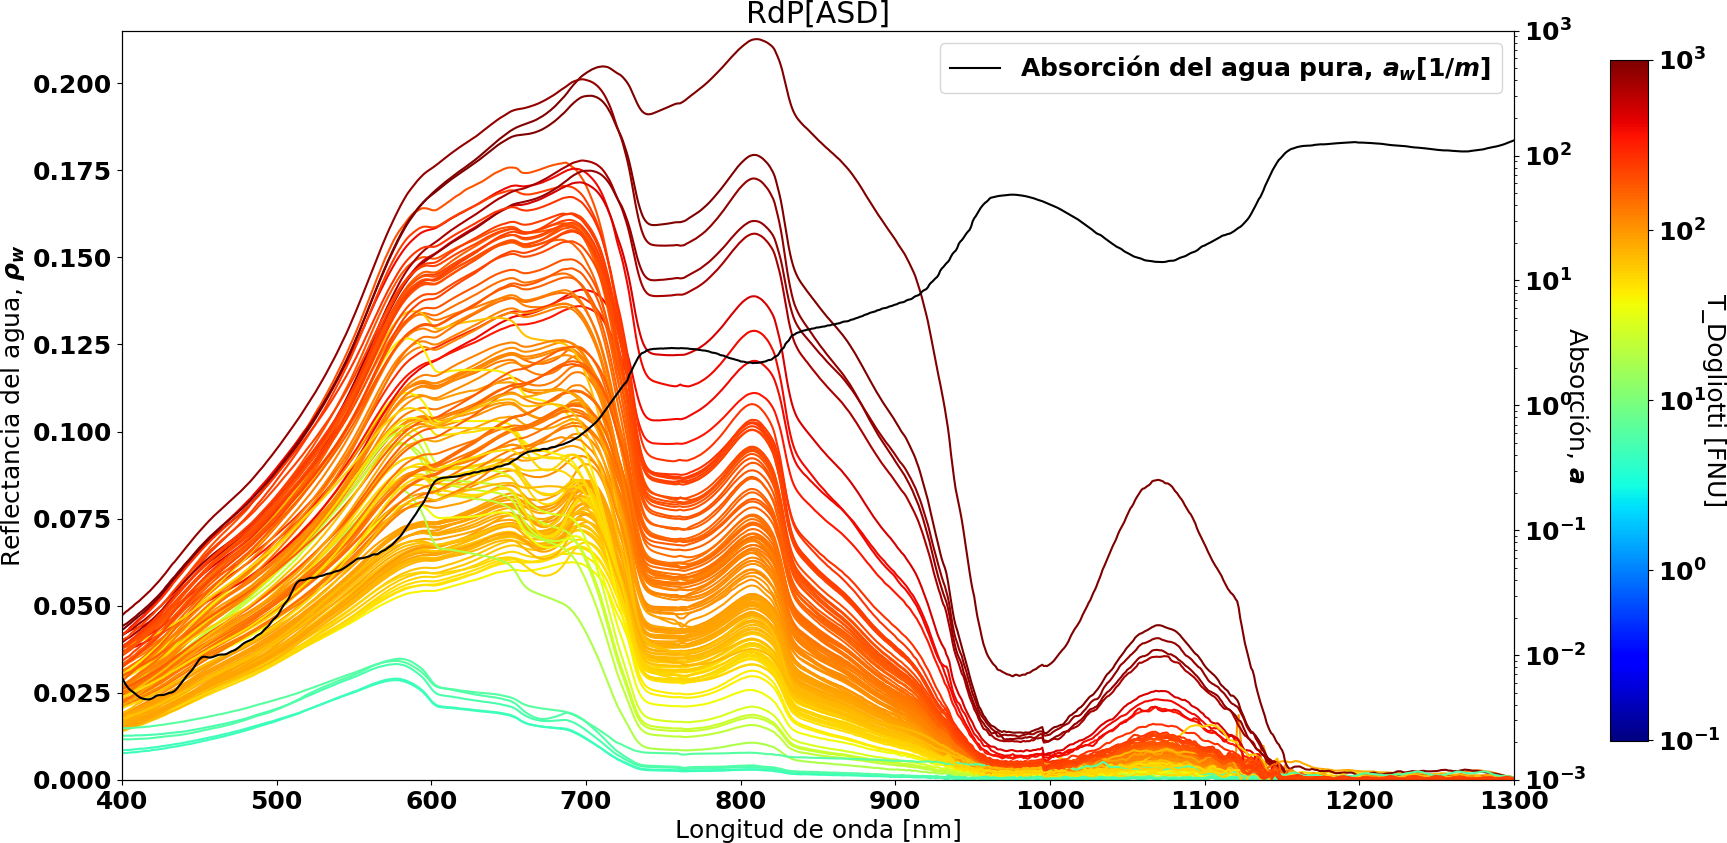
\includegraphics[width=\textwidth]{dat/figures/HyperASD.png}
        \caption[Reflectancias del agua obtenidas con el ASD sobre el RdP]{Reflectancias del agua obtenidas para todo el conjunto de campañas del RdP en que se midió con ASD (todas aquellas que pasaron el control de calidad). Las mismas están mapeadas a un mapa de colores escalado logarítmicamente con la turbidez de Dogliotti et al. 2015, \textit{T\_Dogliotti}. En negro, espectro de absorción del agua líquida pura, \cite{obpg}.}
        \label{dat:HyperASD}
        \end{figure}
    
        Por otro lado, si bien en el rango espectral de 500-700 nm también se observa una fuerte correlación entre las firmas medidas y la absorción del agua, las curvas comienzan a exhibir diferentes comportamientos que se distancian de la similaridad observada en el NIR/SWIR (se observa que las curvas frecuentemente se cortan entre sí). Esto es esperable dado que en este rango espectral el impacto de la eventual presencia de pigmentos y material orgánico coloreado disuelto (CDOM) es mayor y la dependencia espectral de la retrodispersión de partículas no algales más marcada que en el rango NIR/SWIR (véase Figura \ref{dat:HyperTriOS}).
        %
        Por último, en la región del utravioleta, violeta, azul y cian el impacto de la absorción del agua es difícilmente distinguible en las firmas espectrales, dado que entra a dominar en este rango la absorción de las partículas minerales y el CDOM, ambas marcadamente superiores que la del agua en este rango (\S \ref{qssa:s:iops_spm} y \ref{qssa:s:abs_cdom}).
        
        Otra cuestión a destacar de la Figura \ref{dat:HyperASD} es la presencia de firmas espectrales de muy baja turbidez ($\approx 3 FNU$) en comparación con los valores típicos observados en el RdP. Dichas firmas fueron obtenidas en la región de Samborombón (véase Figura \ref{dat:bardp}) en la zona de transición entre los regímen de aguas dulces y turbias de RdP y de aguas saladas del Océano Atlántico.
        También cercano a esta región se conforma el Frente de Turbidez (sobre la Barra del Indio, Framiñan y Brown 1996, \cite{framinan1996}), donde se presentan los valores más altos de turbidez/reflectancia medidos en el RdP (Figura \ref{int:rdp}).

        A partir de la Figura \ref{dat:HyperTriOS} (ídem Figura \ref{dat:HyperASD} pero para el sistema radiométrico TriOS) se pueden visibilizar las principales características distintivas de cada una de las regiones consideradas en el presente análisis. Las firmas del RdP no presentan diferencias sustanciales con las ya analizadas en la Figura \ref{dat:HyperASD}, excepto que en este caso el rango espectral abarcado se restringe a 400-900 nm. En esta figura, aparte del coeficiente de absorción del agua, se superpusieron los coeficientes de absorción específicos de partículas (\S \ref{qssa:s:iops_spm}), de la clorofila-a y la ficocianina, \cite{simis2012}, cuyos impactos son fuertemente observables en las firmas espectrales de Chascomús y en menor medida del Tajo, indicando una concentración más elevada de dichos pigmentos en comparación con el RdP. Nótese que la forma espectral de la absorción de la ficocianina es únicamente identificable en las firmas de Chascomús. Este pigmento es característico de las cianobacterias cuya presencia en esta laguna fue confirmada mediante el análisis al microscopio (\textit{com. pers}. Dra. Laura Sánchez, Laboratorio de Limnología EGE-IEGEBA, UBA/CONICET). Por el contrario, el pico de absorción de la clorofila-a en 680 nm (pigmento presente en todos las algas fotosintetizadoras) genera una depresión en las firmas espectrales de todas las regiones, si bien el efecto es marcadamente más pronunciado en las aguas de dicha laguna, donde la biomasa fitoplanctónica es mayor. A su vez, las aguas del Estuario del Tajo presentan firmas de valores más bajos, debido a concentraciones de SPM más bajas y un impacto fuerte de la clorofila-a. El impacto de la absorción de la ficocianina en las firmas de este estuario no es discernible del impacto de la absorción del agua líquida pura.
    
        \begin{figure}
        \centering
        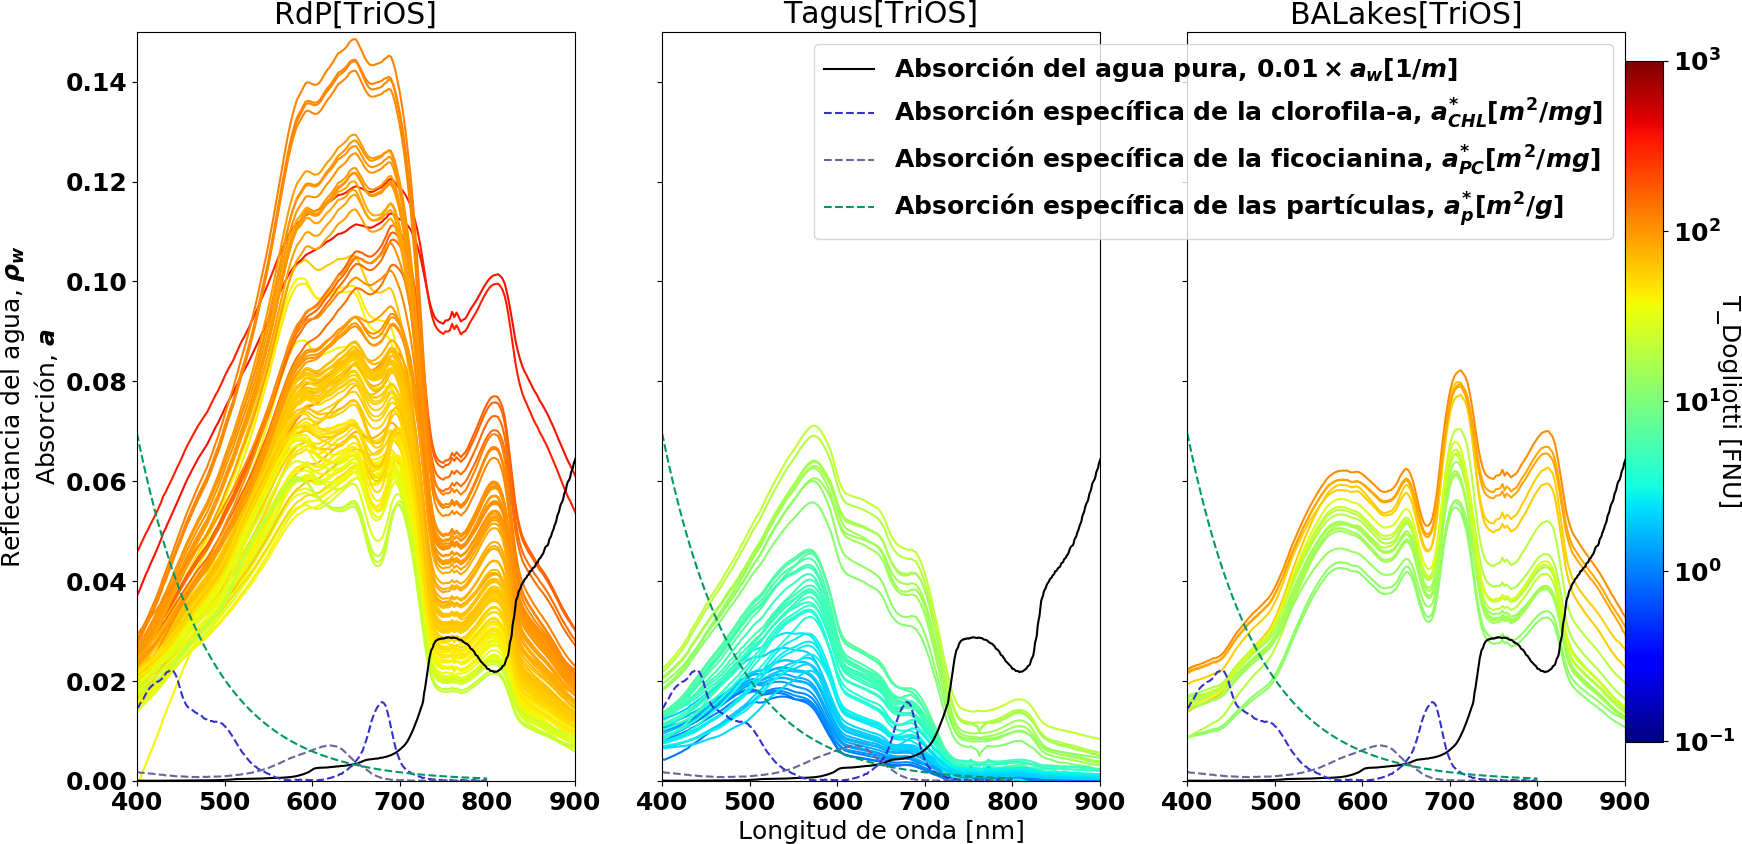
\includegraphics[width=\textwidth]{dat/figures/HyperTriOS.png}
        \caption[Reflectancias del agua medidas con el sistema radiométrico TriOS para las tres regiones consideradas: Río de la Plata, Estuario del Tajo y Laguna de Chascomús.]{Reflectancias del agua medidas con el sistema radiométrico TriOS para las tres regiones consideradas: Río de la Plata (RdP), Estuario del Tajo (Tagus) y Chascomús (BALakes). Se muestran a su vez espectros medios de absorción del agua líquida pura y absorciones específicas típicas de la clorofila-a (\S \ref{qssa:s:abs_pigmentos}), la ficocianina (\S \ref{qssa:s:abs_pigmentos}) y de partículas (\S \ref{qssa:s:iops_spm}).}
        \label{dat:HyperTriOS}
        \end{figure}

    \subsection{Intercomparación de mediciones no espectrales}
    \label{dat:s:noespectrales}
        
        Los rangos abarcados por cada una de las magnitudes no espectrales mencionadas en las secciones anteriores se visualizan en forma de diagramas de cajas en la Figura \ref{dat:boxplot}. En general, se observan valores más elevados de turbidez y SPM para el RdP y Chascomús en comparación con el Estuario del Tajo y un rango dinámico mayor en el RdP en comparación con las restantes. Esto último es esperable dado que el RdP abarca escenarios ópticos mucho más diversos que las otras regiones consideradas y aparte el número de estaciones realizadas excede ampliamente a los de las restantes regiones (véase Cuadro \ref{dat:tab:noespectrales}). A su vez la fracción de materia orgánica respecto de la total (SOM/SPM, también reportada en la Figura \ref{dat:SOMvsSPM}) es menor en el RdP en comparación con el Tajo y Chascomús.

        \begin{figure}
        \centering
        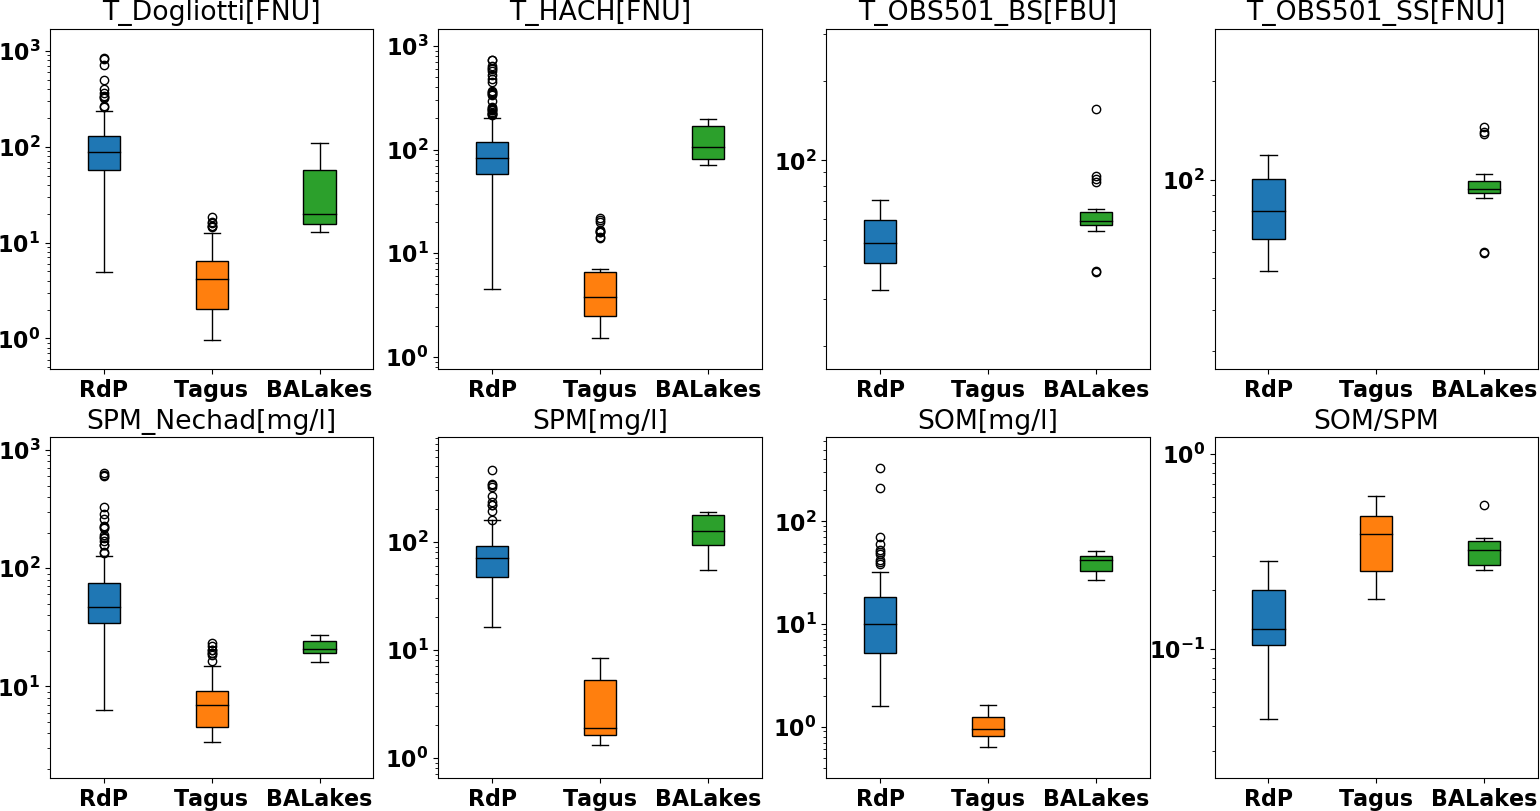
\includegraphics[width=\textwidth]{dat/figures/boxplot.png}
        \caption[Diagramas de cajas de las variables de campo no espectrales según región: Río de la Plata, Laguna de Chascomús y Río Tajo.]{Diagramas de cajas de las variables de campo no espectrales analizadas en este capítulo, divididas según región: Río de la Plata (RdP), Río Tajo (Tagus) y Laguna de Chascomús (BALakes).}
        \label{dat:boxplot}
        \end{figure}

        Prosiguiendo con el análisis, se eligieron algunas combinaciones de a pares de las variables no espectrales mencionadas cuya relación resulta de interés. Para estudiar dicha relación, se evaluó la linealidad entre las variables de dichos pares mediante el regresor lineal no paramétrico de Theil-Sen (Sen 1968, \cite{sen1968}, Theil et al. 1992, \cite{theil1992}). Dicho regresor difiere del convencional de cuadrados mínimos dado que está construido utilizando medianas, es decir, que será menos sensible a la presencia de anomalías. El Cuadro \ref{dat:tab:noespectrales} resume los resultados obtenidos para todos los pares de magnitudes considerados.

        La Figura \ref{dat:T_DogliottivsT_HACH} muestra la relación entre la turbidez estimada por el algoritmo de Dogliotti et al. 2015 (Ec. \ref{dat:eq:dogliotti2015}) y la medida \textit{in situ} por el HACH. Se observa una muy buena correspondencia entre sendas variables tanto para el RdP como para el Estuario del Tajo con pendientes y coeficientes de correlación cercanos a 1 y sesgos bajos. Teniendo en cuenta estas dos regiones, el algoritmo estima valores de turbidez con buena precisión en un rango dinámico de tres órdenes de magnitud [1 - 1000] FNU. En cuanto a la Laguna de Chascomús, si bien la correlación es alta, la estimación no resulta tan adecuada en términos globales (pendiente de $0.69$, sesgo de $-36.82$ FNU), resultando en una subestimación general de la turbidez. Interpretamos que esto ocurre para estas aguas debido a la fuerte presencia de pigmentos absorbentes en la banda roja de 645 nm (una de las utilizadas por el algoritmo de Dogliotti et al. 2015, Ec. \ref{dat:eq:dogliotti2015}). Dicho algoritmo fue calibrado con datos de campo de aguas moderada a altamente turbias; pero los sitios altamente turbios utilizados (RdP, Girondo y Guyana Francesa) no poseen tanto fitoplancton como la Laguna de Chascomús; por lo que sería necesario pensar una recalibración del algoritmo para contemplar estos escenarios, o bien redeterminar el régimen de transición lineal entre las bandas del rojo y la del NIR (llamado $\omega$ en Ec. \ref{dat:eq:dogliotti2015}).

        \begin{figure}
        \centering
        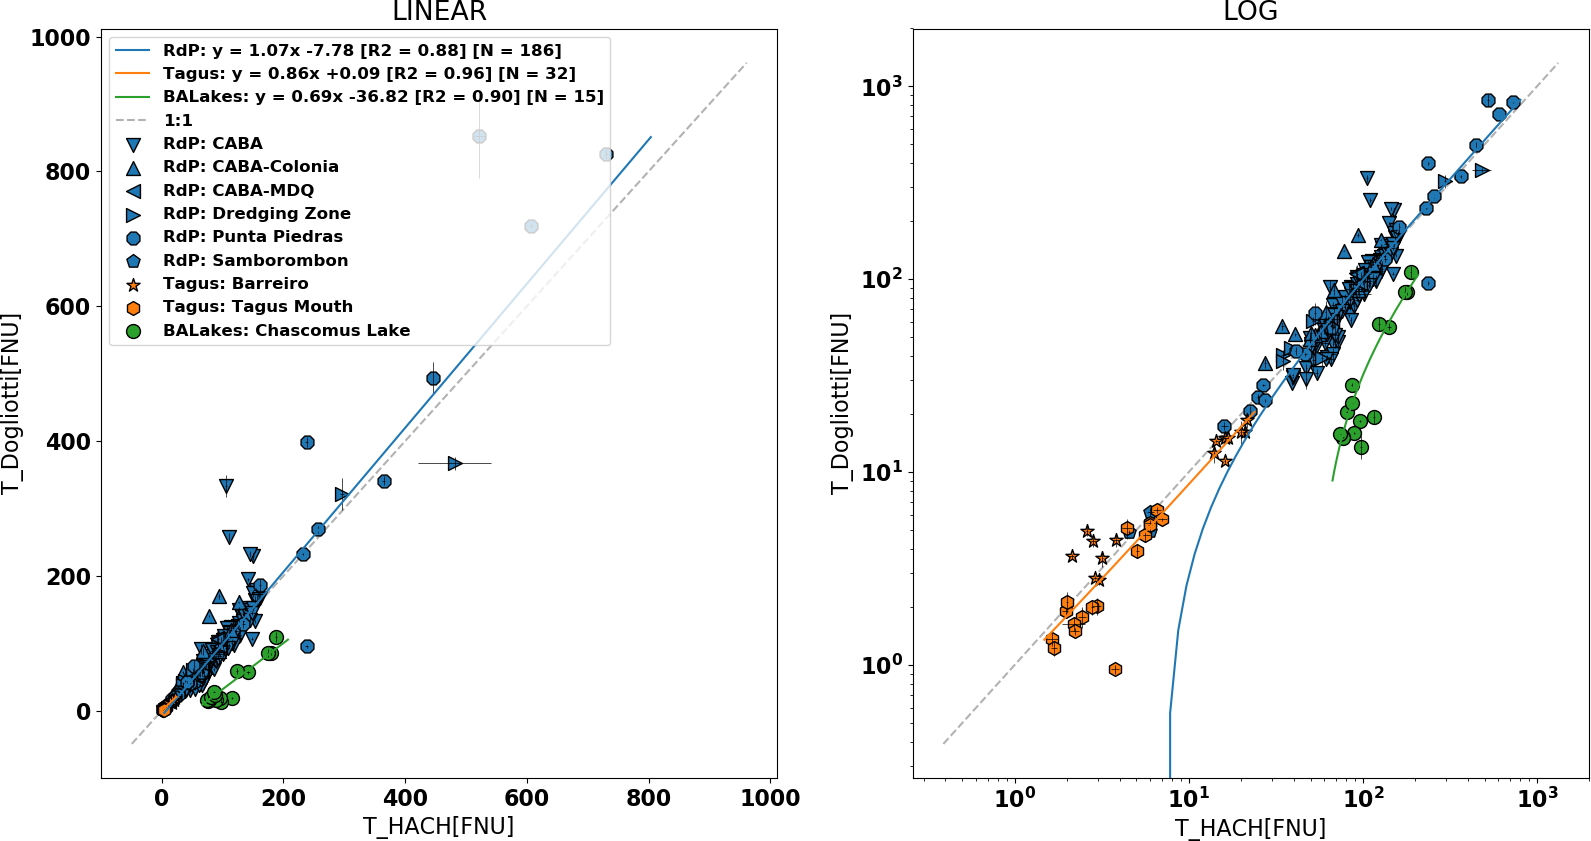
\includegraphics[width=\textwidth]{dat/figures/ScatterT_DogliottivsT_HACH.png}
        \caption[Relación entre la turbidez estimada a partir de reflectancias de agua de campo (T\_Dogliotti) vs. turbidez medida con el turbidímetro HACH.]{Relación entre la turbidez estimada a partir de reflectancias de campo (T\_Dogliotti) vs. turbidez medida con el turbidímetro HACH para las regiones consideradas. Escalas lineal (a) y logarítmica (b). El ajuste lineal fue hecho mediante el regresor no paramétrico de Theil-Sen (insensible a anomalías).}
        \label{dat:T_DogliottivsT_HACH}
        \end{figure}

        El resultado de la validación del algoritmo de una banda de Nechad et al. 2010 utilizado para determinar SPM es muy diferente al anterior (Figura \ref{dat:SPM}), dado que en este caso la correlación entre los valores observados (SPM) y estimados (SPM\_Nechad) resulta muy baja para valores altos de SPM. El coeficiente de correlación para el caso del RdP resultó de $R^{2}=0.02$, y si bien el mismo da razonablemente alto para la Laguna de Chascomús ($R^{2}=0.89$), la pendiente y el sesgo obtenidos están muy alejados del par ideal $(1;\,0\,mg/l)$ - resultó $(0.07;\,13.78\,mg/l)$. El único sitio considerado donde el estimador de Nechad et al. 2010 da buenos resultados es el Estuario del Tajo (pendiente de $0.93$, sesgo de $2.40$ $mg/l$ y correlación de $R^{2}=0.94$). Dicho comportamiento general era esperable, dado que el algoritmo fue diseñado con la banda del rojo en aguas dominadas por partículas minerales. En las aguas del RdP, dicha banda \textit{satura}, es decir que alcanza un comportamiento asintótico que se traduce en una baja sensibilibilidad del algoritmo para detectar diferencias de SPM. Por otro lado, al igual que lo ocurrido con el algoritmo de turbidez, en las aguas de la Laguna de Chascomús dicha banda se halla dominada por el efecto de la absorción del fitoplancton, lo que se traduce en una subestimación de la dispersión de partículas, implicando una subestimación sistemática en los valores de SPM.

        \begin{figure}
        \centering
        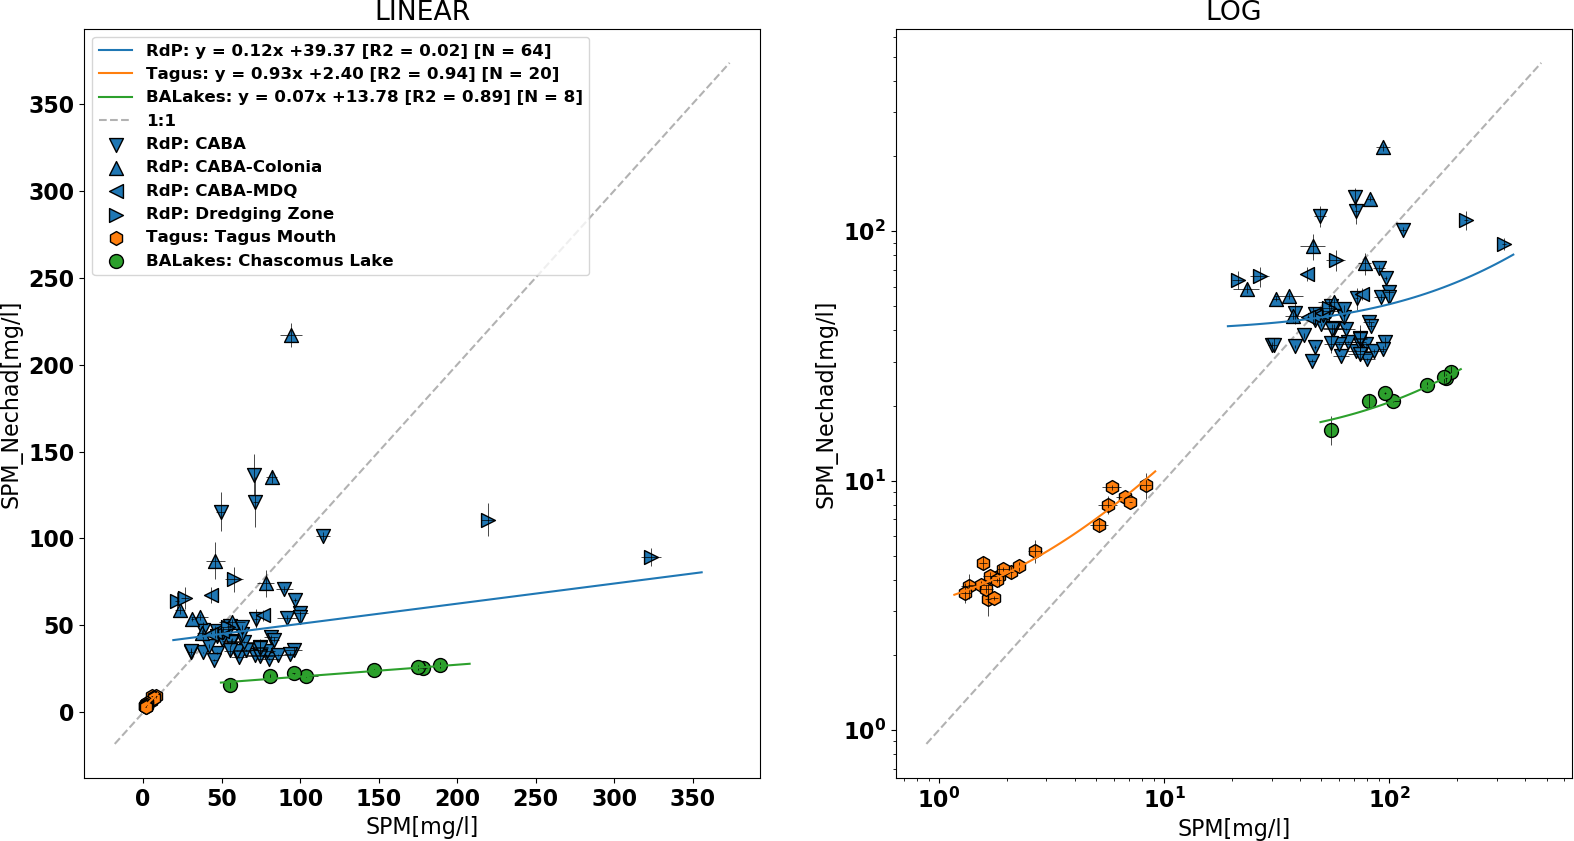
\includegraphics[width=\textwidth]{dat/figures/ScatterSPM_NechadvsSPM.png}
        \caption[Relación entre la concentración de material particulado en suspensión a partir de reflectancias de campo (SPM\_Nechad) y medido \textit{in situ}.]{Ídem Figura \ref{dat:T_DogliottivsT_HACH} pero para la relación entre la concentración de material particulado en suspensión a partir de reflectancias de campo (SPM\_Nechad) y medido \textit{in situ}.}
        \label{dat:SPM_NechadvsSPM}
        \end{figure}
        
        Por otro lado, aparte de considerar el cociente de material orgánico y total ($SOM/SPM$) individual por estación y evaluar su rango de variabilidad (Figura \ref{dat:boxplot}), se obtuvieron valores representativos de dicha fracción mediante una regresión lineal con ordenada nula para cada región (Figura \ref{dat:SOMvsSPM}). Dichas regresiones muestran una fracción de materia orgánica elevada en los casos de Chascomús y Tajo ($32\%$ y $39\%$) y baja en el caso del RdP ($13\%$). Es importante destacar que \textit{a priori} era esperable hallar un comportamiento variable para dicha fracción dentro del RdP, pero de la Figura \ref{dat:SOMvsSPM} no se evidencian diferentes regímenes al considerar las diferentes subregiones (\textit{CABA}, \textit{CABA-Colonia}, etc.).

        \begin{figure}
        \centering
        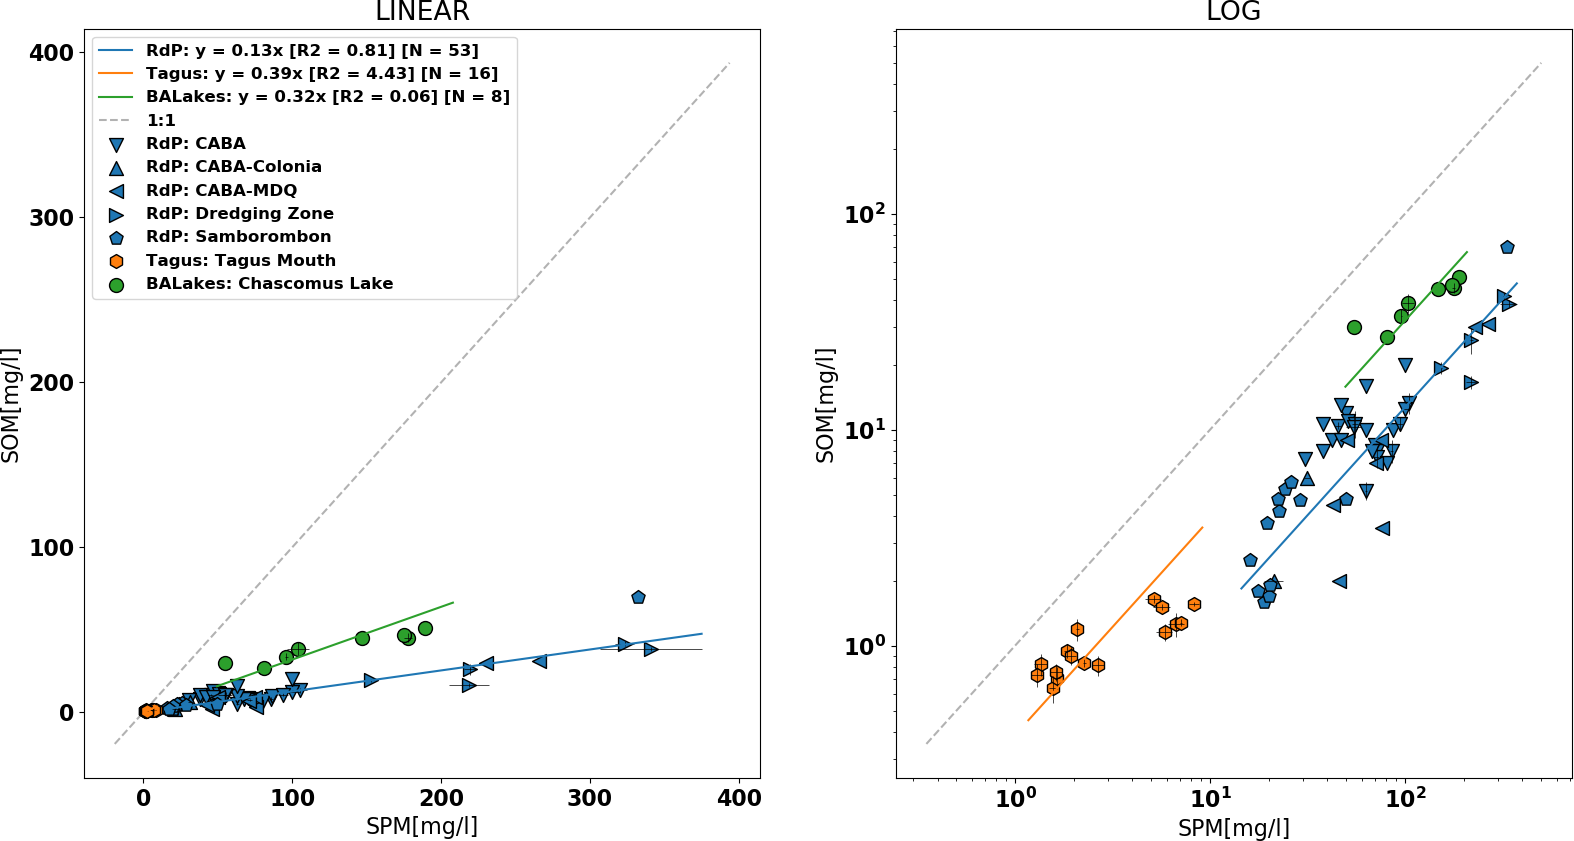
\includegraphics[width=\textwidth]{dat/figures/ScatterSOMvsSPM.png}
        \caption[Relación entre las concentraciones de material particulado en suspensión orgánico (SOM) vs. total (SPM).]{Ídem Figura \ref{dat:T_DogliottivsT_HACH} pero para la relación entre las concentraciones de material particulado en suspensión orgánico (SOM) vs. total (SPM).}
        \label{dat:SOMvsSPM}
        \end{figure}
        
        Como bien es descrito en Dogliotti et al. 2015, \cite{dogliotti2015} (véanse también Moreira et al. 2013, \cite{moreira2013}, Novoa et al. 2017, \cite{novoa2017}, entre otros), la relación entre la turbidez y el SPM muestra una gran variabilidad de un lugar a otro dependiendo de la naturaleza, la forma y el tamaño de las partículas. Por ejemplo, Gohin 2011, \cite{gohin2011}, encuentra una pendiente de $1.85$ FNU.l/mg para las áreas de Dunkerque y Boulogne (sur del Mar del Norte y al este del Canal de la Mancha); Snedden et al. 2007, \cite{snedden2007}, reportan una pendiente de $0.89$ FNU.l/mg para el estuario de Breton (río Mississippi), y Petus et al. 2010, \cite{petus2010}, estiman un valor de $0.74$ FNU.l/mg en las aguas de la costa vasca (Río Adour). Este valor coincide con el hallado por nosotros para el RdP de $0.74$ FNU.l/mg, que a su vez es muy similar al hallado previamente por Moreira et al. 2013 para esta región, de $0.73$ FNU.l/mg. Tanto para el Tajo como para Chascomús, dicho coeficiente es mayor ($0.89$ FNU.l/mg y $1.00$ FNU.l/mg, resp.). Si bien dicha relación es un parámetro distintivo del tipo (tamaño y composición) de partículas presentes en cada uno de los cuerpos de agua considerados, un análisis exhaustivo que pretenda explicar dichas diferencias excede los propósitos de esta tesis.

        \begin{figure}
        \centering
        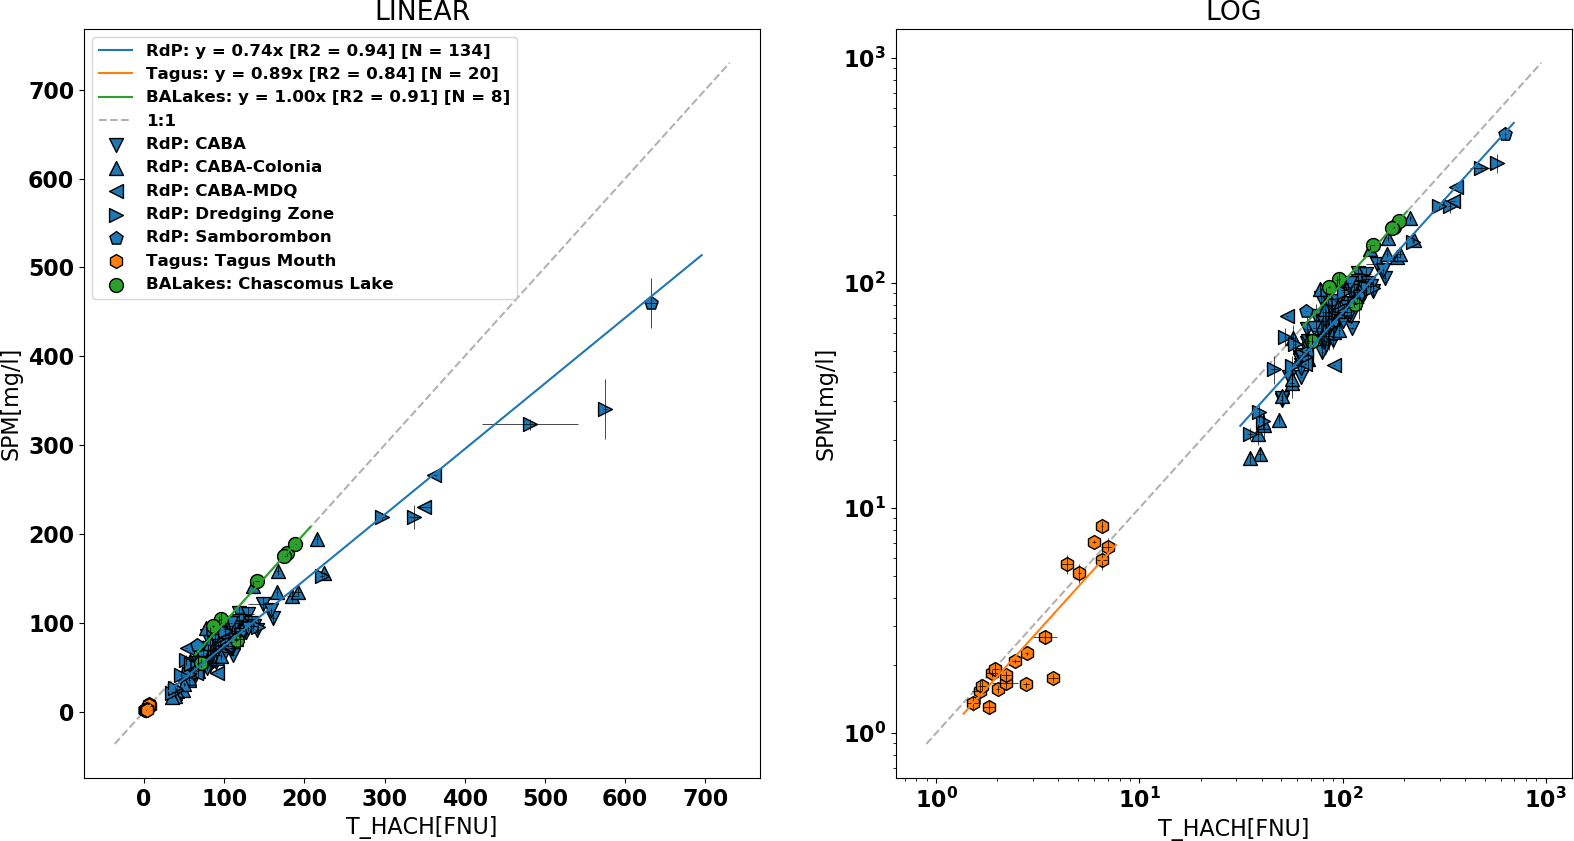
\includegraphics[width=\textwidth]{dat/figures/ScatterSPMvsT_HACH.png}
        \caption[Relación entre SPM y turbidez medida por el turbidímetro HACH.]{Ídem Figura \ref{dat:T_DogliottivsT_HACH} pero para la relación entre SPM y turbidez medida por el turbidímetro HACH.}
        \label{dat:SPMvsT_HACH}
        \end{figure}
        
        Por último, se comparan, a modo de caracterización, las relaciones entre los valores de turbidez obtenidos para cada uno de los medidores de turbidez utilizados (Figuras \ref{dat:T_OBS501_SSvsT_OBS501_BS} y \ref{dat:T_OBS501_SSvsT_HACH}). Se observa una relación lineal entre T\_OBS501\_BS y T\_OBS501\_SS (retrodispersómetro y nefelómetro del OBS501), aunque no se observan diferencias significativas en dicha relación al comparar el RdP con la Laguna de Chascomús (no hay datos de OBS501 disponibles para el Estuario del Tajo), con pendientes de $1.84$ FBU/FNU y $1.71$ FBU/FNU y sesgos de $1.84$ FBU y $1.71$ FBU. Por otro lado, los valores de $T\_OBS501\_SS$ y $T\_HACH$ se asemejan fuertemente para la región del RdP (pendiente $0.91$ FNU/FNU, sesgo $8.56$ FNU y correlación $0.92$), sin embargo presentan fuertes diferencias para la Laguna de Chascomús (pendiente $0.46$ FNU/FNU, sesgo $57.42$ FNU y correlación $0.81$). Si bien el número de puntos que se dispone para Chascomús no es suficiente [$N = 17$] para brindar un resultado conclusivo, también es cierto que \textit{a priori} dichos valores no tienen que coincidir, dado que son medidos mediante métodos diferentes a pesar de tener las mismas unidades: las fuentes son levemente diferentes y aparte el OBS501\_SS es un nefelómetro mientras que el HACH 2100Q \textit{is} es un turbidímetro.
        
        \begin{figure}
        \centering
        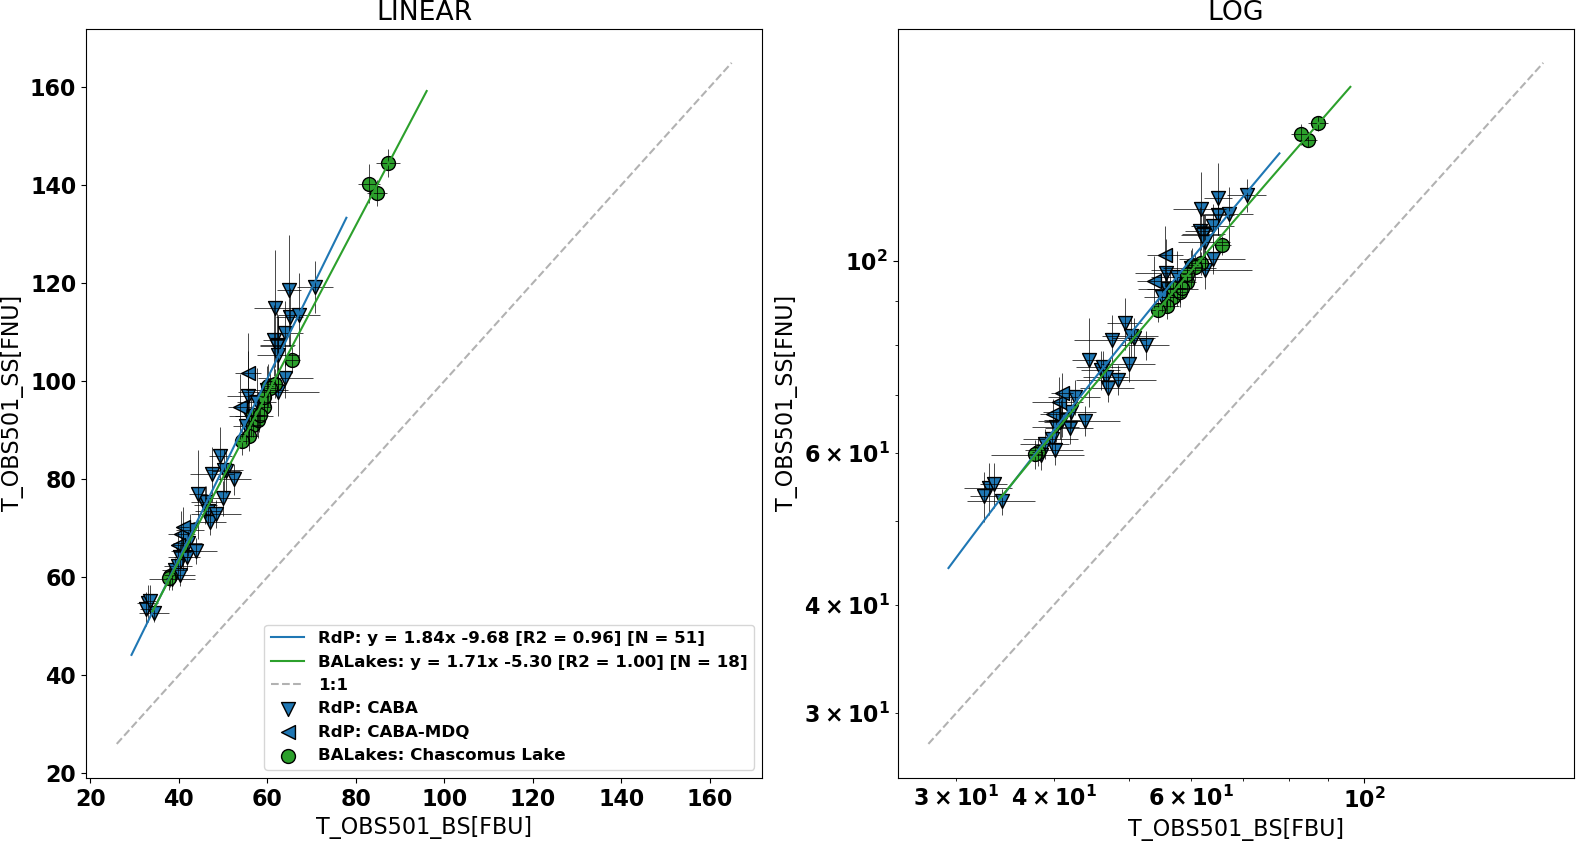
\includegraphics[width=\textwidth]{dat/figures/ScatterT_OBS501_SSvsT_OBS501_BS.png}
        \caption{Ídem Figura \ref{dat:T_DogliottivsT_HACH} pero para la relación entre la turbidez medida por el nefelómetro (T\_OBS501\_SS) vs. el retrodispersómetro (T\_OBS501\_BS) del OBS501.}
        \label{dat:T_OBS501_SSvsT_OBS501_BS}
        \end{figure}
        
        \begin{figure}
        \centering
        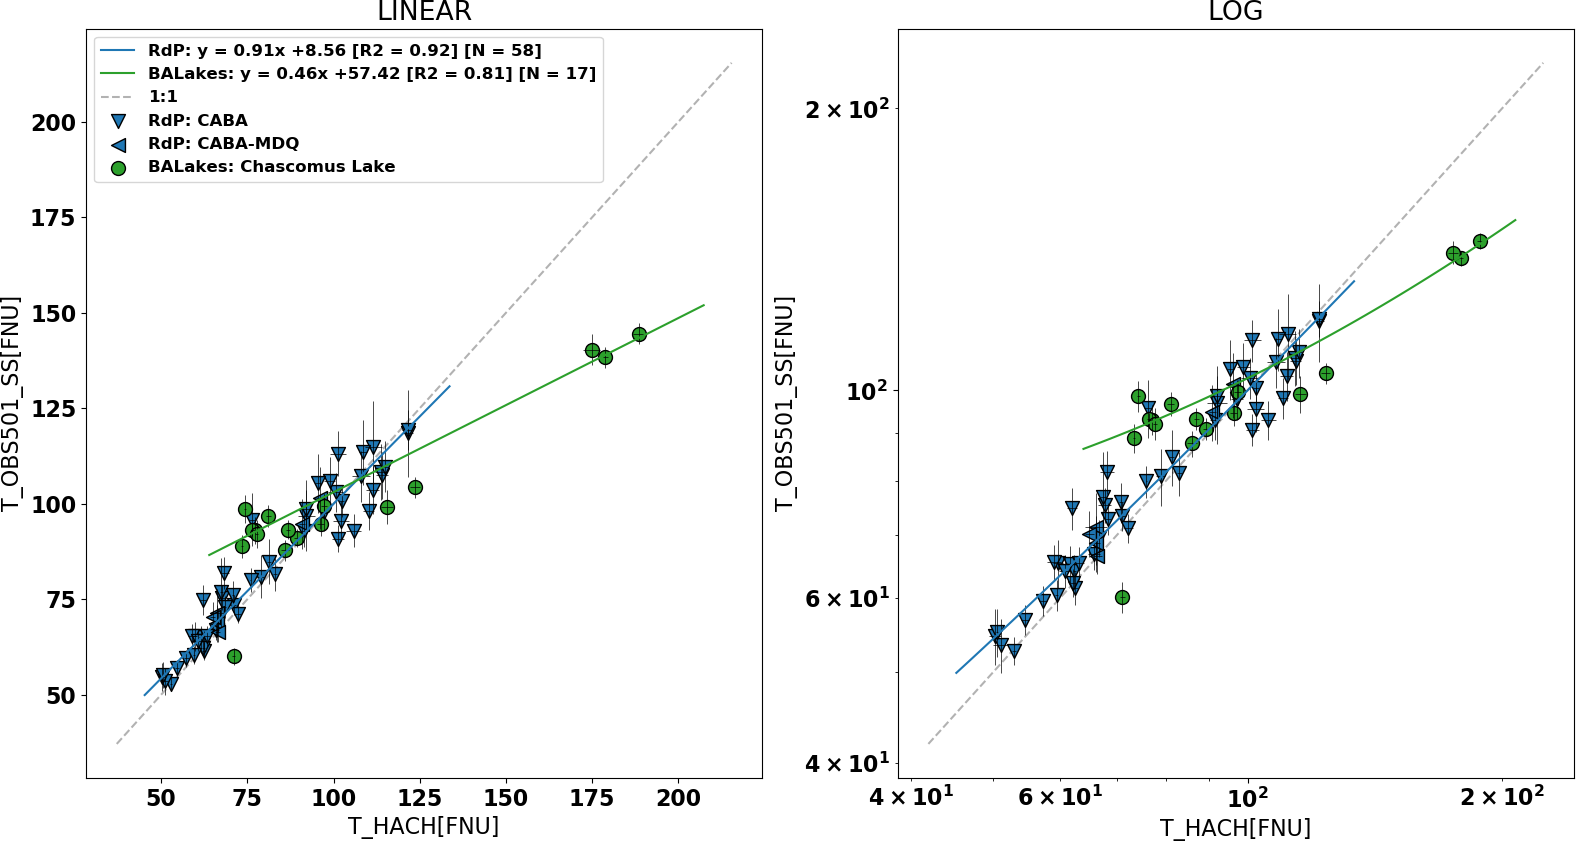
\includegraphics[width=\textwidth]{dat/figures/ScatterT_OBS501_SSvsT_HACH.png}
        \caption[Relación entre valores de turbidez medidos con el nefelómetro sumergible (T\_OBS501\_SS) y el turbidímetro portátil (T\_HACH).]{Ídem Figura \ref{dat:T_DogliottivsT_HACH} pero para la relación entre valores de turbidez medidos por el nefelómetro sumergible (T\_OBS501\_SS) y el turbidímetro portátil (T\_HACH).}
        \label{dat:T_OBS501_SSvsT_HACH}
        \end{figure}

        \begin{table}
        \caption[Resultados obtenidos para las regresiones lineales para cada uno de los pares de variables de campo medidas y regiones de estudio.]{Resultados - pendiente, sesgo, coeficiente de correlación, desviación absoluta mediana (MAD, Ec. \ref{ppe:eq:mad}) - obtenidos para las regresiones lineales no paramétricas (Regresor de Theil-Sen) para cada uno de los pares de variables y regiones de estudio.}
        \small
        \begin{tabular}{|c|l|l|l|l|l|l|}
        \hline
        \multicolumn{1}{|l|}{\textbf{Variables}}                                                                                 & \textbf{Región}                         & \textbf{Pendiente}          & \textbf{Sesgo}                & \textbf{R2}                  & \textbf{MAD} & \textbf{N} \\ \hline
                                                                                                                                 & {\color[HTML]{3531FF} \textbf{RdP}}     & 1.07                        & -7.78                         & 0.877                        & 45.30        & 186        \\ \cline{2-7} 
                                                                                                                                 & {\color[HTML]{F56B00} \textbf{Tagus}}   & 0.86                        & 0.09                          & 0.956                        & 3.05         & 32         \\ \cline{2-7} 
        \multirow{-3}{*}{\textbf{\begin{tabular}[c]{@{}c@{}}T\_Dogliotti{[}FNU{]}\\ vs.\\ T\_HACH{[}FNU{]}\end{tabular}}}        & {\color[HTML]{009901} \textbf{BALakes}} & {\color[HTML]{FE0000} 0.69} & {\color[HTML]{FE0000} -36.82} & 0.899                        & 23.51        & 15         \\ \hline
                                                                                                                                 & {\color[HTML]{3531FF} \textbf{RdP}}     & {\color[HTML]{FE0000} 0.12} & {\color[HTML]{FE0000} 39.37}  & {\color[HTML]{FE0000} 0.020} & 10.48        & 64         \\ \cline{2-7} 
                                                                                                                                 & {\color[HTML]{F56B00} \textbf{Tagus}}   & 0.93                        & 2.40                          & 0.939                        & 1.06         & 20         \\ \cline{2-7} 
        \multirow{-3}{*}{\textbf{\begin{tabular}[c]{@{}c@{}}SPM\_Nechad{[}mg/l{]}\\ vs.\\ SPM{[}mg/l{]}\end{tabular}}}           & {\color[HTML]{009901} \textbf{BALakes}} & {\color[HTML]{FE0000} 0.07} & {\color[HTML]{FE0000} 13.78}  & 0.893                        & 3.45         & 8          \\ \hline
                                                                                                                                 & {\color[HTML]{3531FF} \textbf{RdP}}     & 0.74                        & 0 (fijo)                      & 0.941                        & 28.53        & 134        \\ \cline{2-7} 
                                                                                                                                 & {\color[HTML]{F56B00} \textbf{Tagus}}   & 0.89                        & 0 (fijo)                      & 0.836                        & 1.33         & 20         \\ \cline{2-7} 
        \multirow{-3}{*}{\textbf{\begin{tabular}[c]{@{}c@{}}SPM{[}mg/l{]}\\ vs.\\ T\_HACH{[}FNU{]}\end{tabular}}}                & {\color[HTML]{009901} \textbf{BALakes}} & 1.00                        & 0 (fijo)                      & 0.908                        & 42.95        & 8          \\ \hline
                                                                                                                                 & {\color[HTML]{3531FF} \textbf{RdP}}     & 0.91                        & 8.56                          & 0.923                        & 19.14        & 58         \\ \cline{2-7} 
                                                                                                                                 & {\color[HTML]{F56B00} \textbf{Tagus}}   &                             &                               &                              &              &            \\ \cline{2-7} 
        \multirow{-3}{*}{\textbf{\begin{tabular}[c]{@{}c@{}}T\_OBS501\_SS{[}FNU{]}\\ vs.\\ T\_HACH{[}FNU{]}\end{tabular}}}       & {\color[HTML]{009901} \textbf{BALakes}} & {\color[HTML]{FE0000} 0.46} & {\color[HTML]{FE0000} 57.42}  & 0.812                        & 8.99         & 17         \\ \hline
                                                                                                                                 & {\color[HTML]{3531FF} \textbf{RdP}}     & 1.84                        & -9.68                         & 0.955                        & 18.64        & 51         \\ \cline{2-7} 
                                                                                                                                 & {\color[HTML]{F56B00} \textbf{Tagus}}   &                             &                               &                              &              &            \\ \cline{2-7} 
        \multirow{-3}{*}{\textbf{\begin{tabular}[c]{@{}c@{}}T\_OBS501\_SS{[}FNU{]}\\ vs.\\ T\_OBS501\_BS{[}FBU{]}\end{tabular}}} & {\color[HTML]{009901} \textbf{BALakes}} & 1.71                        & -5.30                         & 0.995                        & 10.13        & 18         \\ \hline
                                                                                                                                 & {\color[HTML]{3531FF} \textbf{RdP}}     & 0.13                        & 0 (fijo)                      & 0.812                        & 5.16         & 53         \\ \cline{2-7} 
                                                                                                                                 & {\color[HTML]{F56B00} \textbf{Tagus}}   & 0.39                        & 0 (fijo)                      & 4.430                        & 0.62         & 16         \\ \cline{2-7} 
        \multirow{-3}{*}{\textbf{\begin{tabular}[c]{@{}c@{}}SOM{[}mg/l{]}\\ vs.\\ SPM{[}mg/l{]}\end{tabular}}}                   & {\color[HTML]{009901} \textbf{BALakes}} & 0.32                        & 0 (fijo)                      & 0.062                        & 14.08        & 8          \\ \hline
        \end{tabular}
        \label{dat:tab:noespectrales}
        \end{table}

\section{Conclusiones}
\label{dat:s:conclusiones}
    
    En este capítulo se presentaron los datos de campo disponibles para el área de estudio de la presente tesis - el RdP - y se los comparó con datos bioópticos obtenidos en otras áreas de estudio exploradas por nuestro grupo de investigación - el estuario del Tajo en Portugal y la Laguna de Chascomús en la Provincia de Buenos Aires - con el fin de extraer similitudes y rasgos distintivos de las mediciones del RdP. Dichas regiones de estudio difieren ópticamente del RdP esencialmente en concentración (Tajo) y en contenido de material orgánico (Tajo y Chascomús). Se exhibió la distribución geográfica de las estaciones realizadas en en RdP y en dichas regiones y se hizo una descripción de cada una de las magnitudes medidas: reflectancias del agua mediante mediciones radiométricas (ASD y TriOS), turbidez mediante diferentes turbidímetros (HACH y OBS501) y determinación de la concentración de masa en volumen de material particulado en suspensión (SPM) mediante el método gravimétrico aplicado sobre muestras filtradas de agua. A su vez, se describieron los instrumentos utilizados, sus protocolos de medición y procesamiento. También, a partir de las reflectancias del agua, se computaron los algoritmos de turbidez de Dogliotti et al. 2015, \cite{dogliotti2015}, y de SPM de Nechad et al. 2010, \cite{nechad2010} para poder validar dichos algoritmos en nuestra región de estudio.
    
    Por otro lado, se describió el método que fue utilizado para sistematizar los datos de campo en una base de datos relacional, para lo cual fue necesario organizar los datos en forma de campos y entradas con una llave identificatoria única (estaciones). La sistematización de la base de datos - incluyendo la realización de los códigos para procesar los datos adquiridos durante las campañas - y el análisis de los mismos se realizó mediante el módulo \textit{pandas} del lenguaje \textit{Python}, cuyo desempeño resultó óptimo en nuestro caso, dado que es un lenguaje de alto nivel - es decir, intuitivo pero no necesariamente el más veloz - y a su vez el volumen de datos no excede los tamaños recomendables para \textit{pandas} ($\approx 50 GB$). En caso de que la base de datos continúe expandiéndose (por ej. aumentar en un factor 10 ó más su tamaño) será necesario abordar los datos con lenguajes específicos de bases de datos, como \textit{SQL} (\textit{Structured Query Language}). Los principales códigos generados para procesar, sistematizar y analizar los datos de campo se hallan en \href{https://github.com/juanchossn/scripts_tesis_doctoral}{\textbf{\underline{este repositorio}}}\cite{repo}.
    
    Los resultados obtenidos para el conjunto total de las mediciones son compatibles con lo esperado. Se observan rasgos espectrales distintivos del RdP con respecto al Tajo y a Chascomús: valores de reflectancias en el rojo/NIR/SWIR más elevados que en Tajo y Chascomús; un impacto marcadamente menor debido a la absorción de pigmentos fotosintéticos, y al igual que en Tajo y Chascomús, una elevada correlación negativa entre la forma espectral de las reflectancias y la absorción del agua en el rojo/NIR/SWIR.
    Por otro lado, se observan valores típicos de turbidez y SPM similares entre el RdP y la Laguna de Chascomús ($\approx 80$ FNU y $\approx 80$ mg/l), a su vez marcadamente mayores a los observados en el Estuario del Tajo ($\approx 5$ FNU y $\approx 2$ mg/l). Asimismo, se observan fracciones de material orgánico a total (SOM/SPM) menores en el RdP ($13\%$) en comparación con Chascomús y Tajo ($32\%$ y $39\%$, respectivamente), situación ya discernible del análisis de las diferencias entre las firmas espectrales ya descritas. A su vez, se observa una relación entre la turbidez (FNU, HACH) y SPM en el RdP de $0.74$ FNU.l/mg, muy similar a la ya encontrada por Moreira et al. 2013 de $0.73$ FNU.l/mg para nuestra región de estudio.
    
    Los valores de turbidez estimados por el algoritmo de Dogliotti et al. 2015 son plausibles tanto para el RdP como para el Tajo, abarcando un rango dinámico de 1-1000 FNU; mientras que subestiman los observados en Chascomús. Dicha discrepancia está asociada a un marcado impacto de la absorción de fotopigmentos en la banda del rojo (utilizada por el algoritmo en regímenes de turbidez baja a moderada). El mismo efecto de subestimación se observa al evaluar la estimación de SPM por el algoritmo de Nechad et al. 2010 para la región de Chascomús; aunque este algoritmo tampoco estima bien los valores de SPM en regímenes de altas concentraciones del RdP ($R^{2}=0.02$), resultado esperable dado que no incorpora la transición al NIR para evadir la saturación que sí incorpora el de Dogliotti et al. 2015 para regímenes de turbidez/SPM altos.
    
    Finalmente, se estudiaron las relaciones entre los valores de turbidez estimados por los diferentes medidores de turbidez descritos (turbidímetro HACH y retrodispersómetro y nefelómetro OBS501). Se observan comportamientos lineales con baja ordenada al origen para la relación entre el nefelómetro y el retrodispersómetro del OBS501, sin observarse diferencias significativas entre regiones. Si bien las mediciones de turbidez por dispersión a $90\degree$ del OBS501 y del HACH (ambas en unidades nefelométricas de formazina, FNU, y dentro de los requerimientos de la ISO 7027) son consistentes para el RdP (pendiente de 0.91 FNU/FNU, sesgo de 8.56 FNU y correlación de $R^{2}=0.92$), presentan diferencias significativas en las aguas de la Laguna de Chascomús (pendiente de 0.46 FNU/FNU, sesgo de 57.42 FNU y correlación de $R^{2}=0.81$). Si bien es cierto que se necesitarían más datos para evaluar mejor dicha correspondencia (actualmente, $N = 17$), también es cierto que, si bien ambas mediciones satisfacen los requerimientos de la ISO 7027 y están referidas a las mismas unidades, no son perfectamente comparables dados sus diferentes métodos de medición (turbidimétrico en caso del HACH y nefelométrico en caso del OBS501\_SS). Aún así, un análisis exhaustivo que pretenda explicar dicha discrepancia excede los objetivos de esta tesis.
    
    Las curvas de reflectancias presentadas y analizadas en este capítulo fueron utilizadas para calibrar y validar el algoritmo presentado en \S \ref{blr} y para validar el algoritmo presentado en \S \ref{pca}. El hecho de haber adquirido y sistematizado una base de datos de campo para las aguas ópticamente complejas del RdP es de un gran potencial para la calibración y validación de futuros algoritmos bioópticos desarrollados para nuestra región de interés.
\chapter[CA sobre imágenes OLCI basada en BLRs]{Corrección atmosférica de imágenes OLCI sobre aguas turbias basada en las bandas roja, NIR y SWIR y una técnica de Residuos de Líneas de Base (BLR)}
\label{blr}

% , un enfoque común para la corrección atmosférica píxel a píxel de las imágenes satelitales de color del mar es calcular las reflectancias del agua y de aerosoles en dos bandas espectrales, típicamente en el infrarrojo cercano (NIR, 700-1000 nm) o en el infrarrojo de onda corta (SWIR, 1000-3000 nm), y luego extrapolar la reflectancia de aerosoles a longitudes de onda más cortas. Para aguas claras, esto se puede lograr simplemente utilizando las bandas NIR, donde la reflectancia del agua se puede suponer insignificante, es decir, el supuesto de \textit{agua negra} (o \textit{píxel negro}, cf. \S \ref{int:s:ACblackPixelNIR}). Para aguas moderadamente turbias, donde la reflectancia del agua en el NIR no es más despreciable, es necesario modelar la reflectacnia en el NIR (\S \ref{int:s:ACiterNIR}) o utilizar bandas SWIR - es decir, de longitud de onda más larga - donde el supuesto de agua negra continúa siendo válido incluso para aguas como las del RdP (\S \ref{int:s:ACnirswir} y \ref{int:s:ACswir}). Como mencionamos anteriormente, para aguas extremadamente turbias, el modelado de la reflectancia del agua no nula en el NIR se vuelve incierto porque las pendientes espectrales de las reflectancias del agua y de aerosoles se vuelven similares en este rango, lo que dificulta la distinción entre ellas. 
%
Tal como vimos en el capítulo \ref{int}, en el sensoramiento remoto de aguas extremadamente turbias como las del RdP el uso de bandas SWIR para la CA está claramente establecido - por ejemplo, las bandas MODIS en 1240 nm y 2130 nm - aunque tales bandas SWIR no se hallan presentes en muchos sensores como el Ocean and Land Color Instrument (OLCI). En este sensor, en cambio, una nueva banda SWIR - más económica - a 1016 nm está disponible con potencial para mejorar la calidad de la corrección atmosférica sobre aguas extremadamente turbias. Ese potencial es analizado en el presente capítulo, donde demostramos que para los tripletes de bandas espectralmente cercanas (como las bandas OLCI a 779-865-1016 nm), la reflectancia corregida por Rayleigh de la banda intermedia de cada triplete luego de haber sustraído la \textit{línea de base}, aquí denominado \textit{Residuo de la Línea de Base} (BLR, \textit{BaseLine Residual}) es esencialmente independiente de las condiciones atmosféricas. Utilizamos tres BLRs definidos por los tres tripletes de bandas consecutivas del grupo de bandas 620-709-779-865-1016 nm (es decir, 620-709-779, 709-779-865 y 779-865-1016 nm) para calcular la reflectancia del agua y, por lo tanto, la reflectancia de los aerosoles en estas longitudes de onda. Mostramos que al comparar el desempeño del algoritmo aquí propuesto con otros algoritmos de corrección atmosférica para el RdP, se observa un rendimiento similar en aguas moderadamente turbias y claras y una mejora considerable en aguas extremadamente turbias.

$\quad$
\noindent

El contenido del presente capítulo se halla parcialmente publicado en:

$\quad$
\noindent

GOSSN, J.I.; RUDDICK, KEVIN G.; DOGLIOTTI, ANA I. (2019) Atmospheric correction of OLCI imagery over extremely turbid waters based on the red, NIR and 1016 nm bands and a new baseline residual technique. Remote Sensing.: MDPI AG. 2019 vol.11 nr. 3. pp. 2072-4292, \cite{gossn2019}

\section{Introducción}
\label{blr:s:introduction}

    El Ocean and Land Color Instrument (OLCI) es un sensor cuya misión es la observación de los continentes y de color del mar, actualmente a bordo de los satélites Sentinel-3 A y B, conformando parte del plan espacial Copernicus de la Agencia Espacial Europea (\textit{European Space Agency} ESA). Sus bandas espectrales y tecnología radiométrica (ver \S \ref{ppe}) fueron heredadas de la misión MERIS con el agregado de bandas en el violeta (400 nm) y en el SWIR (1016 nm). Esto quiere decir que el mismo posee las bandas que poseía MERIS necesarias para los algoritmos de CA basados en procedimientos extrapolativos en el NIR (\S \ref{int:s:ACiterNIR}).
    
    Recapitulando lo que vimos en \S \ref{int}, estos algoritmos pueden fallar para aguas extremadamente turbias del Río de la Plata (por ejemplo, casos en que $\rho_{w}(865 nm)>0.02 $ con valores de SPM superiores a $100g/m^{3}$), debido a uno o más de los siguientes problemas:
    
    \begin{enumerate}

        \item[] \textbf{P1}. El espectro de reflectancia del agua en el NIR se vuelve más \textit{plano} o \textit{blanco} (Doxaran et al. 2002, \cite{doxaran2002}) y, por lo tanto, más similar a los espectros de reflectancia de aerosoles (Ruddick y Vanhellemont 2015, \cite{ruddick2015});
    
        \item[] \textbf{P2}. Con una reflectancia alta, los modelos analíticos simples de reflectancia del agua en el NIR, tales como expansiones polinómicas del parámetro de Gordon (el cociente $\frac{b_{b}}{a + b_{b}}$) ya no son precisos (Ruddick et al. 2006, \cite{ruddick2006}) y se necesita un mejor modelado (Lee et al. 2016, \cite {lee2016}, Luo et al. 2018, \cite {luo2018});
    
        \item[] \textbf{P3}. La reflectancia a tope de la atmósfera (TOA) puede incluso superar los valores de saturación de los fotodetectores de ciertos sensores de color del mar, lo que hace que estas longitudes de onda sean inutilizables (Dogliotti et al. 2011,\cite {dogliotti2011}).
    
    \end{enumerate}
    
    En estos casos, como ya hemos visto, se necesitan mejoras en el procedimiento estándar de extrapolación al NIR. Como fue explicitado en \S \ref{int:s:ACswir}, un enfoque es aplicar el supuesto de agua negra en las bandas del SWIR (por ejemplo, 1240, 1640 y 2130 nm en MODIS, como investigaremos en \S \ref{pca}), donde la absorción de agua es mucho mayor,  resultando en reflectancias del agua prácticamente nulas incluso en aguas extremadamente turbias (Wang y Shi 2005, \cite{wang2005}). Aunque el sensor OLCI carece de bandas SWIR lejanas (por ejemplo, 1240 nm, 2130 nm en MODIS), incorpora una nueva banda SWIR en 1016 nm (nominalmente 1020 nm, aunque aquí se prefiere el valor de 1016 nm, que corresponde a la longitud de onda media de la SRF de la banda). Si bien el supuesto de agua negra no es válido en 1016 nm para aguas extremadamente turbias (Knaeps et al. 2012, \cite{knaeps2012}), la absorción del agua pura es mucho mayor en esta banda ($a_{w}(1016)=29.57 m^{-1}$ Kou et al. 1993, \cite{kou1993}) que en el NIR ($a_{w}(865)=4.6 m^{-1}$ Kou et al. 1993, \cite{kou1993}), lo que significa que el achatamiento del espectro de reflectancia del agua en el NIR en aguas extremadamente turbias (P1) no se extiende a 1016 nm. Esto quiere decir que, con la inclusión de esta banda, los espectros de reflectancia del agua tienen una forma claramente diferente de los espectros de reflectancia de aerosoles y la descomposición de la reflectancia a TOA (o corregida por Rayleigh) en componentes provenientes del agua y de los aerosoles es factible. 
    
    A su vez, el potencial operativo de los enfoques de espectro completo (\S \ref{int:s:ACacoplados}) es plenamente reconocido, pero aquí se prefiere el enfoque extrapolativo porque cada paso del proceso tiene una base física clara, lo que facilita la identificación y resolución de eventuales inconvenientes. Por ejemplo, un modelo de reflectancia de agua deficiente, una calibración imprecisa o un modelo de aerosoles inapropiado se harán evidentes con un enfoque extrapolativo, pero pueden ser menos obvios con un enfoque de sistema agua-atmósfera acoplado de espectro completo.
    
    En este capítulo, presentamos el diseño de un algoritmo de corrección de aerosoles píxel a píxel para aguas turbias en las bandas OLCI del rango rojo-NIR-SWIR (RNS) mediante la identificación de \textit{invariantes atmosféricos} que son sensibles a la reflectancia del agua pero insensibles a los aerosoles (véase Philpot 1991,\cite{philpot1991}).
    %
    Este enfoque se basa en el hecho de que en la región RNS, la reflectancia de los aerosoles es espectralmente más suave que la reflectancia del agua (Ruddick y Vanhellemont 2015, \cite{ruddick2015}). Para calcular directamente la reflectancia del agua, suponiendo únicamente que la reflectancia de aerosoles es espectralmente suave, se propone aquí un algoritmo de Residuo de la Línea de Base (\textit{Baseline Residual}, BLR) para reflectancias corregidas por Rayleigh en 3 tripletes de bandas en el rango RNS. Se define el BLR a partir de restarle al valor de reflectancia de la longitud de onda intermedia (p.ej 709 nm en el triplete 620-709-779 nm) la altura del segmento que une las reflectancias de longitud de onda más corta y más larga del triplete (p.ej el segmento que une a las reflectancias en 620 nm y 779 nm en el triplete 620-709-779 nm). Es decir que el BLR es el residuo de la reflectancia intermedia respecto de la línea de base conformada por las reflectancias laterales (una medida de la \textit{concavidad} de la reflectancia). Este enfoque es similar al adoptado, por ejemplo, en el producto de Altura de la Línea de Fluorescencia (\textit{Fluorescence Line Height}, FLH, Letelier y Abott 1996, \cite{letelier1996}) y proporciona una cantidad, el BLR, que es invariante frente a la adición de señales espectralmente lineales (o suficientemente suaves). Al calcular tres BLRs atmosféricos diferentes, definidos por las reflectancias corregidas por Rayleigh ($\rho_{RC}$, \S \ref{int:s:rayleigh}) en los tripletes (620-709-779 nm), (709-779-865 nm) y (779-865-1016 nm), y aplicando sobre ellos un factor de corrección de \textit{transmitancia equivalente} es posible calcular la reflectancia del agua en el RNS píxel a píxel, incluso en los casos de aguas extremadamente turbias.

    Una vez que se calcula la reflectancia del agua en el rango RNS, la CA puede retrotraerse a los algoritmos extrapolativos NIR estándar al sustraer la reflectancia del agua de la reflectancia corregida por Rayleigh, lo cual permite determinar la reflectancia de aerosoles en el RNS y por ende permitir estimar un tipo de aerosol y concentración en el NIR y el consecuente uso de modelos tabulados para extrapolar la reflectancia de aerosoles a todas las longitudes de onda como en Gordon y Wang 1994, \cite{gordon1994}. Alternativamente, en caso de no requerirse una CA de espectro completo, es posible usar la reflectancia de agua RNS directamente para estimar productos como la turbidez (Dogliotti et al. 2015, \cite{dogliotti2015}, Dogliotti et al.2016, \cite{dogliotti2016}, \S \ref{dat:s:turbidez}) o SPM (Nechad et al. 2010, \cite{nechad2010}, Shen et al. 2010, \cite{shen2010}, Moreira et al. 2013, \cite{moreira2013}, \S \ref{dat:s:spm}), o la concentración de clorofila-a en aguas turbias (Gilerson et al. 2010, \cite{gilerson2010}, Gitelson 1992, \cite{gitelson1992}, Gons et al. 2005, \cite{gons2005})

\section{Materiales y métodos}
\label{blr:s:materials}

    Las siguientes subsecciones describen los diferentes conjuntos de datos utilizados para calibrar y validar el algoritmo.

    \subsection{Mediciones radiométricas \textit{in situ}}
    \label{blr:s:insitu}
    
        En el presente capítulo, se utilizaron mediciones radiométricas \textit{in situ} sobre la superficie (véase \S \ref{dat:s:radiometricas}) para los siguientes propósitos:
        
        \begin{enumerate}
            \item Como entrada a un conjunto de simulaciones de transferencia radiativa para calcular un factor de transmitancia que se aplicará a los BLRs (véase \S \ref{blr:s:transmittance}),
            \item Para comparar entre BLRs de los datos \textit{in situ} y de los derivados de OLCI (véase sección \ref{blr:s:results:blrs}), y
            \item Para validar las reflectancias del agua obtenidas - aplicando la CA aquí descrita y otras preexistentes - sobre imágenes OLCI simultáneas con mediciones \textit{in situ} en el RdP (ejercicio de \textit{match-up}).
        \end{enumerate}
        
        Para los primeros dos propósitos, se seleccionó un total de 105 mediciones de reflectancia del agua de varias campañas (2012-2015) realizadas en el RdP con el radiómetro ASD. La razón por la que se usaron dichas mediciones y no las del TriOS es que el rango espectral de este último no cubre la banda de OLCI en 1016 nm (véase \S \ref{dat:s:radiometricas}). El protocolo de medición, procesamiento y control de calidad de las mediciones sigue exactamente lo detallado en \S \ref{dat:s:asd}, al cual se le agregó el control de calidad opcional hecho sobre el coeficiente de variación en el rango $400-900$ nm y a $1016$ nm (Ec. \ref{dat:eq:CV}). El subconjunto de reflectancias espectrales del agua que pasaron los criterios antes mencionados se representa en la Figura \ref{blr:blrRcSosVsblrWAsd}a.

        Para el propósito de realizar el ejercicio de \textit{match-up} se utilizaron mediciones \textit{in situ} hechas con el radiómetro TriOS - el único disponible durante las campañas con pasadas del sensor OLCI - siguiendo también los protocolos descritos en el capítulo \S \ref{dat}. El sitio de validación utilizado correspondió, en los cuatro casos donde fue posible el \textit{match-up}, al Muelle del Club de Pescadores de Palermo, localizado en $(-34.560754; -58.39881)$ en la costa de la Ciudad de Buenos Aires (sitio perteneciente al conjunto de datos denominado \textit{RdP: CABA} en las figuras de la \S \ref{dat:s:resultados}). Para el \textit{match-up} se utilizaron ventanas cuadradas de 3px $\times$ 3px de las imágenes, cuyos píxeles centrales están desfasados en dos píxeles hacia el interior del RdP para evitar el impacto de la presencia del muelle en las ventanas. Los detalles de las estaciones, las imágenes utilizadas y el desfasaje están reportados en el Cuadro \ref{blr:tab:matchups}.

    \subsection{Simulaciones de Transferencia Radiativa}
    \label{blr:s:simulations}
    
        Se realizaron simulaciones de transferencia radiativa para comparar el comportamiento de los BLRs calculados a partir de reflectancias del agua, $BLR(\rho_{w})$, y BLRs calculados a partir de reflectancias RC, $BLR (\rho_{RC})$, y también para establecer un factor de transmitancia equivalente que se aplicará a los BLRs calculados a partir de reflectancias RC de escenas OLCI (véase \S \ref{blr:s:transmittance}). Para ello se utilizó el código CNES-SOS v5.0 (Centro Nacional de Estudios Espaciales-Órdenes Sucesivos de Dispersión, Lenoble et al. 2007, \cite{lenoble2007}, \S \ref{sos}). Las 105 mediciones radiométricas \textit{in situ} descritas anteriormente se utilizaron como entrada al código para analizar cómo los BLRs de reflectancias del agua (definidos en las Ecs. \ref{blr:eq:blr}-\ref{blr:eq:baseline}) se relacionan con los BLRs de reflectancias corregidas por Rayleigh teniendo en cuenta la transmitancia atmosférica.
        
        Combinando todos los espectros \textit{in situ} con un conjunto de múltiples condiciones atmosféricas simuladas, se calcularon un total de 70875 espectros de reflectancia corregidos por Rayleigh (RC) (Cuadro \ref{blr:tab:sos}) con el código CNES-SOS, que corresponde a: 3 ángulos cenitales solares y de observación a $0\degree$, $ 30\degree$ y $60\degree$ (interpolados desde los ángulos de cuadratura gaussiana, \cite{lenoble2007}), 5 ángulos de acimut relativos al sol en el rango $0-180\degree$ (paso de $45\degree$, donde $0\degree$ representa observar sobre el \textit{sunglint} directo), 3 granulometrías de aerosoles e índices de refracción de tipo Continental (WMO-C), Marítimo (WMO-M) y Urbano (WMO -U), correspondientes a los modelos ópticos de aerosoles descritos en \S \ref{int:s:wmo}, 5 profundidades ópticas de aerosoles a 500 nm en el rango 0-0.4 (paso 0.1) y 105 reflectancias de agua \textit{in situ} (\S \ref{blr:s:insitu}, Figura \ref{blr:blrRcSosVsblrWAsd} a). El índice de refracción relativo de la interfase agua-aire se fijó en $1.334$ en todo el espectro y la velocidad del viento se fijó en $3 m/s$. Los parámetros que describen la dispersión de Rayleigh de las moléculas de aire fueron fijados de acuerdo con los valores del espesor óptico de Rayleigh y el cociente de depolarización de la Figura \ref{int:rayleigh_tau_depol}. Los perfiles verticales moleculares y de aerosoles se configuraron para seguir las funciones de decaimiento exponencial de escalas características de 8 km y 2 km, respectivamente. El código se estableció para no exceder 20 órdenes de dispersión e incluir los efectos de la polarización.
        
        \begin{table}
        \caption{Parámetros atmosféricos, superficiales, geométricos y espectrales utilizados como entrada para el conjunto de simulaciones CNES-SOS utilizado en el presente capítulo.}
        \centering
        %% \tablesize{} %% You can specify the fontsize here, e.g.  \tablesize{\footnotesize}. If commented out \small will be used.
        \begin{tabular}{|c|c|c|}
        \hline
        \textbf{Parámetro CNES-SOS}	& \textbf{Valores de entrada}\\
        \hline
        $\lambda$ (Longitud de onda) & 615-1040 nm (paso 5 nm)\\
        \hline
        $\theta_{s}$ (Ángulo cenital solar) & $0\degree-60\degree$ (paso $30\degree$)\\
        \hline
        $\theta_{v}$ (Ángulo cenital de observación) & $0\degree-60\degree$ (paso $30\degree$)\\
        \hline
        $\phi$ (Ángulo acimutal relativo) & $0\degree-180\degree$ (paso $45\degree$)\\
        \hline
        $\rho_{w}$ (Reflectancia del agua) & ASD \textit{in situ} (RdP)\\
        \hline
        $w$ (Intensidad del viento) & 3 m/s\\
        \hline
        $n_{w}$ (Índice de refracción relativo aire-agua) & 1.334\\
        \hline
        $\tau_{r}$ (Espesor óptico Rayleigh) & Bodhaine et al. 
        1999, \cite{bodhaine1999}\\
        \hline
        $\delta_{r}$ (Cociente de depolarización molecular) & Bodhaine et al. 
        1999, \cite{bodhaine1999}\\
        \hline
        $H_{r}$ (Escala de \textit{e-folding} molecular) & 8 km\\
        \hline
        $\tau_{a}$ (Espesor óptico de aerosoles a 500 nm) & 0:0.1:0.4\\
        \hline
        $dV_{a}/dlnr$ (Granulometría de aerosoles) & WMO-C, -M, -U, \S \ref{int:s:wmo}\\
        \hline
        $n_{a} + i.m_{a}$ (Índice de refracción de aerosoles) & WMO-C, -M, -U, \S \ref{int:s:wmo}\\
        \hline
        $H_{a}$ (Escala de \textit{e-folding} de aerosoles) & 2 km\\
        \hline
        $n_{max}$ (Máximo orden de dispersión) & 20\\
        \hline
        $I_{pol}$ (Índice de polarización) & 1 (considerar polarización)\\
        \hline
        \end{tabular}
        \label{blr:tab:sos}
        \end{table}
        
        Para obtener las reflectancias corregidas por Rayleigh del conjunto, el código se ejecutó dos veces, al igual que en Gross et al. 2007, \cite{gross2007}: i) utilizando los valores de entrada especificados en el Cuadro \ref{blr:tab:sos} para calcular la reflectancia a TOA ($\rho_{TOA}^{SOS}$), y ii) suponiendo un entorno acuático negro ($\rho_{w}=0$) y sin contenido de aerosoles ($\rho_{a}=0$). Los valores del segundo conjunto se restan a los del primero para calcular la reflectancia RC de la misma forma que se calcularía en el paso de corrección por Rayeigh de un procesador de datos satelitales:

        \begin{equation}
        \rho^{SOS}_{RC} = \rho^{SOS}_{TOA}(Aire + Interfase + Aerosoles + Agua) - \rho^{SOS}_{TOA}(Aire + Interfase)
        \label{blr:eq:sosray}
        \end{equation}

    \subsection{Imágenes de OLCI}
    \label{blr:s:olci}
    
        Las imágenes OLCI L1B y L2 utilizadas en este capítulo se descargaron de la base de datos CODA (Copernicus Online Data Access) el 1 de febrero de 2018, \cite{coda}. Las imágenes L1B y L2 utilizadas en este trabajo corresponden a la línea base de procesamiento v2.23. La lista detallada de escenas de Río de la Plata (RdP), Bahía Blanca (BBl, Argentina) y Costa de Bélgica (BE) utilizadas para calibrar y validar el desempeño del algoritmo - en ausencia de datos \textit{in situ} - se muestra en el Cuadro \ref{blr:tab:olci}. Por otro lado, las imágenes utilizadas para realizar el ejercicio de \textit{match-up} de hallan reportadas en el Cuadro \ref{blr:tab:matchups}.
        
        Antes de proceder con los cálculos de BLR, se aplicaron dos correcciones preliminares a las imágenes L1B. En primer lugar, se realiza una corrección por \textit{EPVs} (Eventos de Partículas Veloces) para eliminar artefactos ocasionales sobre píxeles originados por el impacto de partículas magnetosféricas sobre los sensores, siguiendo lo expuesto en \S \ref{ppe}. En segundo lugar, se aplica la corrección por Rayleigh (\S \ref{int:s:rayleigh}), utilizando SeaDAS v7.5 (Bailey et al. 2010, \cite{bailey2010}, Stumpf et al. 2003, \cite{stumpf2003}), para eliminar la radiancia atmosférica esperable para una atmósfera enteramente dominada por dispersión Rayleigh provocada por moléculas de aire y con mar negro de fondo (aunque también considera la reflexión especular de la superficie). El producto que se obtiene es la reflectancia corregida por Rayleigh (RC) en todas las bandas de interés de OLCI, denominado $\rho_{s}$ en SeaDAS.
        
        \begin{table}
        \small
        \caption{Lista de imágenes OLCI (L1B, procesamiento de base v2.23) del Río de la Plata (RdP), de la Costa Belga (BE) y de Bahía Blanca (BBl) usadas para calibrar y validar el algoritmo, descritas por fecha y horario de adquisición.}
        \begin{tabular}{|l|l|l|l|l|}
        \hline
        \textbf{Región} & \textbf{Tiempo de adquisición} & \makecell[tl]{\textbf{Ventana(s) de}\\ \textbf{Calibración/} \\ \textbf{Validación}} & \makecell[tl]{\textbf{Corrección}\\\textbf{Atmosférica}\\\textbf{a Ventana Fija}\\\textbf{(Fix-AC)}} & \textbf{Cal/Val}\\
        \hline
         & yyyy-mm-ddThh:mm:ssZ & líneas; píxels & líneas; píxels & Cal\\
        \hline
        RdP & 2016-08-17T12:55:02Z & 1347-1636; 1258-1528 & 1750-1764; 1143-1157 & Cal\\
        \hline
        RdP & 2016-11-10T12:51:59Z & 1057-1446; 521-685 & 1598-1612; 567-581 & Cal\\
        \hline
        RdP & 2016-11-29T12:58:49Z & 1643-1796; 1218-1332 & 2117-2131; 1267-1281 & Cal\\
        \hline
        RdP & 2017-01-14T13:06:26Z & 2254-2589; 838-1052 & 2655-2669; 1155-1169 & Cal\\
        \hline
        RdP & 2017-03-13T13:02:29Z & \makecell[tl]{1890-2013; 1177-1258\\2044-2124; 1130-1256} & 2140-2154; 1462-1476 & Cal\\
        \hline
        RdP & 2017-05-01T13:32:08Z & \makecell[tl]{4301-4525; 1126-1177\\4381-4561; 1216-1356} & 4549-4563; 1271-1285 & Cal\\
        \hline
        RdP & 2017-07-02T13:24:47Z & 3761-3840; 1220-1254 & 4133-4147; 1498-1512 & Cal\\
        \hline
        RdP & 2017-10-15T13:02:34Z & 1586-1927; 1088-1182 & 2460-2474; 1635-1649 & Cal\\
        \hline
        RdP & 2017-11-19T12:54:31Z & \makecell[tl]{1355-1576; 2252-2366\\1367-1718; 2108-2247\\862-1262; 2025-2108} & 1895-1909; 2178-2192 & Cal\\
        \hline
        BE & 2016-07-19T10:00:32Z & 1613-1823; 1525-1649 & 1497-1511; 1790-1804 & Val\\
        \hline
        BBl & 2016-10-09T13:22:33Z & 2359-2701; 970-1094 & 2917-2931; 1077-1091 & Val\\
        \hline
        RdP & 2017-10-31T12:47:47Z & 724-927; 1398-1452 & 1104-1118; 1774-1788 & Val\\
        \hline
        RdP & 2017-01-21T13:24:42Z & Todo RdP & No aplicada & Val\\
        \hline
        RdP & 2016-06-08T13:09:51Z & Todo RdP & No aplicada & Val\\
        \hline
        RdP & 2017-12-12T12:59:01Z & Todo RdP & No aplicada & Val\\
        \hline
        \end{tabular}
        \label{blr:tab:olci}
        \end{table}

        \begin{table}
        \small
        \caption{Listado de \textit{match-ups} sobre el RdP analizados: sitio de adquisición, ID de estación \textit{in situ}, tiempo de adquisición de imagen OLCI y desfasaje temporal entre la imagen OLCI y la medición de campo correspondiente.}
        \begin{tabular}{|l|l|l|l|l|}
        \hline
        \textbf{ID} & \textbf{Sitio} & \textbf{ID de estación} & \begin{tabular}{c} \textbf{Tiempo de} \\ \textbf{adquisición OLCI} \end{tabular} &  \begin{tabular}{c} \textbf{Desfasaje} \\ \textbf{temporal} \end{tabular}\\ \hline
        \textbf{A}              & Muelle de Palermo & RdP\_20170106\_M0117-02 & 2017-01-06T13:14:16Z       & 4 min                       \\ \hline
        \textbf{B}              & Muelle de Palermo & RdP\_20170126\_test1    & 2017-01-26T12:54:24Z       & 7 min                       \\ \hline
        \textbf{C}              & Muelle de Palermo & RdP\_20180404\_P10      & 2018-04-05T13:43:54Z       & 1 min                       \\ \hline
        \textbf{D}              & Muelle de Palermo & RdP\_20181105\_PTG-P13  & 2018-11-08T13:17:51Z       & 0 min                       \\ \hline
        \end{tabular}
        \label{blr:tab:matchups}
        \end{table}

        Las correcciones atmosféricas estándar de la NASA/SeaDAS y la ESA también se aplicaron a las imágenes OLCI para comparar el rendimiento con el esquema BLR propuesto: i) el software \textit{l2gen} del SeaDAS de la NASA (Bayley et al. 2010, \cite{bailey2010}, Stumpf et al. 2003, \cite{stumpf2003}) se ejecutó con la opción de aerosoles $-2$, es decir, suponiendo un procedimiento iterativo para encontrar el modelo de aerosoles óptimo utilizando las bandas de 865 nm y 1016 nm (denominado SeaDAS-2 (865,1016) en adelante), y ii) la corrección atmosférica estándar de la ESA (realizada para imágenes L2, procesamiento de base v2.23), que combina la corrección atmosférica de base (\textit{Baseline Atmospheric Correction}, BAC, Antoine y Morel 1999,\cite{antoine1999}), que es esencialmente un esquema de píxel negro basado en el NIR, en conjunto con la corrección atmosférica de píxeles brillantes (\textit{Bright Pixel Atmospheric Correction}, BPAC, Moore et al. 1999, \cite{moore1999}), que calcula primero la reflectancia del agua en el NIR desde un enfoque iterativo.

        Por otro lado, para el ejercicio de \textit{match-up} se comparó el desempeño del algoritmo aquí presentado (al cual denominamos BLR-AC) con la CA BAC/BPAC ya descrita anteriormente y con la CA denominada C2RCC (Case 2 Regional processor). La misma es una CA de la familia de algoritmos de espectro completo basada en una red neuronal, originalmente propuesta por Doerffer y Schiller 2007, \cite{doerffer2007}. Originalmente, los parámetros de las capas de \textit{neuronas} de dicha red fueron optimizados a partir de un gran conjunto de simulaciones de transferencia radiativa, que a su vez fueron reentrenados por Brockmann et al. 2016, \cite{brockmann2016}, dando lugar a una nueva CA, aquí denominada C2RCCnewNN, la cual también fue considerada en el ejercicio de intercomparación.
        
        Dado que el conjunto total de estaciones disponibles para realizar el ejercicio de \textit{match-up} con OLCI en el RdP es muy reducido (un total de 4 estaciones), las posibilidades de realizar análisis estadístico sobre los resultados es muy reducida. Aún así, utilizaremos el error absoluto medio (\textit{Mean Absolute Error}, MAE), definido como 

        \begin{equation}
            MAE = \frac{1}{N}\sum_{i=1}^{N} |\hat{x}_{i}-x_{i}|
            \label{blr:eq:MAE}
        \end{equation}

        \noindent donde $\hat{x}_{i}$ y $x_{i}$ son los $i$-ésimos valores estimado y observado, respectivamente, y $N$ es el número total de observaciones ($N=4$). En nuestro caso, tomaremos las reflectancias del agua medidas \textit{in situ} como los valores observados y las derivadas de OLCI como los valores estimados (por ej. $x=\rho_{w}(620 nm)^{TriOS}$ y $\hat{x}=\rho_{w}(620 nm)^{C2RCC}$). 

        Aparte del MAE, se utilizó la raíz de la diferencia cuadrática media (\textit{Root Mean Square-Diference}, RMSD) para intercomparar resultados de reflectancia del agua entre diferentes esquemas de CA, definida de manera muy similar al MAE:

        \begin{equation}
            RMSD = \sqrt{\frac{1}{N}\sum_{i=1}^{N} (\hat{x}_{i}-x_{i})^{2}}
            \label{blr:eq:RMSD}
        \end{equation}

    \subsection{Base teórica del algoritmo BLR}
    \label{blr:s:atb}

    % Considérese la siguiente expresión para representar la refectancia total a TOA (cf. Gordon y Wang 1994, Equation 1 \cite{gordon1994}):
    % \begin{equation}
    %     \rho^{TOA} = \pi \frac{L^{TOA} d^{2}}{E^{TOA}cos(\theta_{s})}
    %     \label{blr:eq:rhoTOA}
    % \end{equation}
    
    % \noindent
    % donde $L^{TOA}$ es la radiancia total a TOA, $d$ es la distancia Sol-Tierra en unidades astronómicas, $E^{TOA}$ es la irradiancia solar extraterrestre a TOA y $\theta_{s}$ es el ángulo cenital solar.
    
    % Un primer paso común a todos los esquemas de corrección atmosférica es estimar la reflectancia corregida por Rayleigh ($\rho_{RC}$, véase \S \ref{int:s:rayleigh}):
    
    % \begin{equation}
    %     \rho_{RC} = \rho^{TOA} - \rho_{R}
    %     \label{blr:eq:rhoRC}
    % \end{equation}
    
    El esquema de corrección de aerosoles presentado aquí constituye un enfoque de píxel a píxel basado en el Residuo de Línea de Base (BLR), que es la diferencia entre la señal en una banda \textit{media} (M, es decir, de longitud de onda intermedia en un triplete de bandas) y el valor de la línea de base formada por las señales en las bandas izquierda (L) y derecha (R) en esta longitud de onda media, como se ilustra en la Figura \ref{blr:blrExamples}. En este trabajo, usamos BLRs calculados usando reflectancias corregidas por Rayleigh (RC), por lo que definimos $BLR(\rho_{RC})$ de la siguiente manera:
    
    \begin{equation}
        BLR(\rho_{RC})(\lambda_{L}, \lambda_{M}, \lambda_{R}) = \rho_{RC}(\lambda_{M})-BL(\rho_{RC})(\lambda_{M}|\lambda_{L},\lambda_{R})
        \label{blr:eq:blr}
    \end{equation}
    
    \noindent donde $\lambda_{L}$, $\lambda_{M}$ y $\lambda_{R}$ representan las longitudes de onda menor, intermedia y mayor del triplete, $\rho_{RC}(\lambda_{M}) $ es la reflectancia RC en $\lambda_{M}$ y $BL(\rho_{RC})(\lambda_{M} |\lambda_{L},\lambda_{R}) $ es el término de referencia, dado por:
    
    \begin{equation}
    BL(\rho_{RC})(\lambda_{M}|\lambda_{L},\lambda_{R}) =   \frac{\rho_{RC}(\lambda_{L})(\lambda_{R}-\lambda_{M})+\rho_{RC}(\lambda_{R})(\lambda_{M}-\lambda_{L})}{\lambda_{R}-\lambda_{L}}
    \label{blr:eq:baseline}
    \end{equation}
    
    \begin{figure}
    \centering
    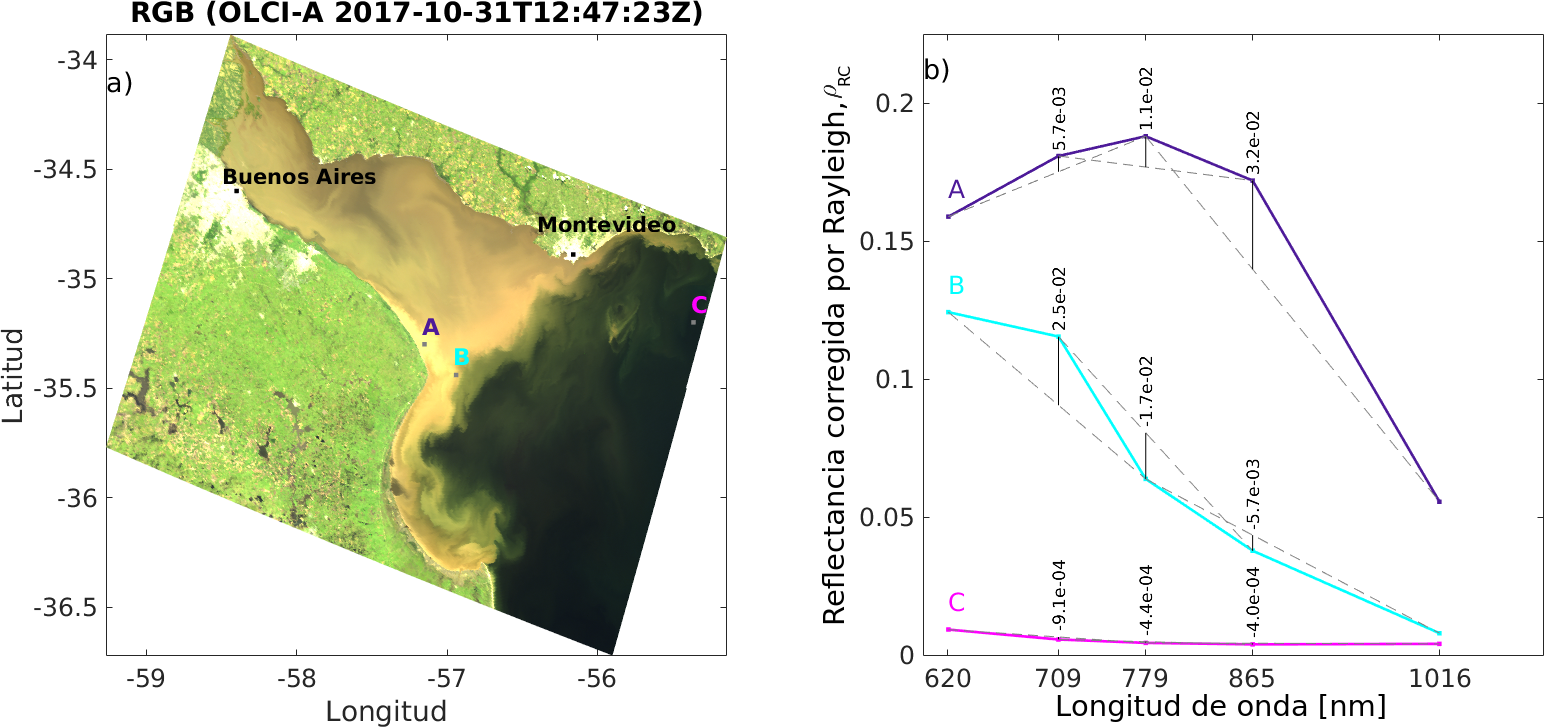
\includegraphics[width=\textwidth]{blr/figures/blrExamles}
    \caption[Ejemplos de BLRs en distintos regímenes de SPM en la imagen OLCI-A 2017-10-31T12:47:23Z sobre el RdP]{a) Composición RGB de la imagen OLCI-A en el Río de la Plata del 2017-10-31T12:47:23Z, creada a partir de reflectancias RC a 620 nm (R) 560 nm (G) y 442 nm (B). b) Reflectancias RC en las bandas roja, infrarroja cercana e infrarroja de onda corta (RNS) utilizadas para el enfoque de corrección atmosférica por BLRs (BLR-AC) en los sitios A, B y C, junto con los correspondientes valores de BLRs.}
    \label{blr:blrExamples}
    \end{figure}
    
    Otros algoritmos preexistentes en la disciplina de color del mar que usan BLRs incluyen la Altura de la Línea de Fluorescencia (\textit{Fluorescence Line Height}, FLH, \cite{letelier1996}), definida para MODIS como el BLR de las radiancias normalizadas del agua en las bandas 665 nm, 677 nm y 746 nm, es decir, $FLH = BLR(nL_{w})(665,677,746)$; el Índice de Algas Flotantes (\textit{Floating Algal Index}, FAI, Hu 2009, \cite{hu2009}), definido también para MODIS como el BLR de las reflectancias corregidas por Rayleigh a 645 nm, 859 nm y 1240 nm, es decir, $ FAI=BLR(\rho_{RC})(645,859,1240)$, el Índice de Máxima Clorofila para MERIS (Maximum Chlorophyll Index, MCI, Gower y King 2008 \cite{gower2008}, véase Ec. \ref{ppe:eq:mci}), que puede expresarse como $MCI=BLR(L_{TOA})(681,709,754)$, o el Índice Sintético de Clorofila (\textit{Synthetic Chlorophyll Index}, SCI, Shen et al. 2010, \cite{shen2010}), que se calcula utilizando reflectancias sensadas remotamente como $SCI=-BLR(R_{rs})(620,665,681)-BLR(R_{rs})(560,620,681)$ (estas bandas corresponden a los casos de MERIS y OLCI). En algunos casos, estos enfoques (FLH, SCI) se implementan después de una corrección de aerosoles, mientras que en otros casos (FAI, MCI) no se aplica.
    
    Sin embargo, todos estos enfoques son similares en el sentido que los índices BLR no se ven esencialmente afectados por señales indeseables como aerosoles y/o \textit{sunglint} moderado (y, por lo tanto, tampoco por errores típicos en el proceso de eliminación de esta señal), ya que estos componentes son generalmente espectralmente más suaves que la señal en el agua, especialmente en la región RNS. Matemáticamente, si consideramos que la señal atmosférica $\rho_{atm}$ dentro del rango espectral determinado por el triplete de bandas $(\lambda_{L},\lambda_{M},\lambda_{R})$ es lo más \textit{suave} posible, es decir, de dependencia lineal con la longitud de onda, $\rho_{atm}(\lambda)=m\lambda+b $, luego $BLR(\rho_{atm})(\lambda_{L},\lambda_{M},\lambda_{R})=0$.
    
    El algoritmo de CA presentado aquí se diseñó teniendo en cuenta que la dependencia de los BLRs con los componentes atmosféricos se minimiza mejor utilizando reflectancias RC en bandas espectralmente cercanas y para longitudes de onda más largas ($\lambda>600nm $), de forma tal de reducir el impacto de la incertidumbre proveniente de la corrección de Rayleigh, incluida la dispersión múltiple acoplada Rayleigh-aerosoles. Esto puede verse considerando la siguiente expresión para la reflectancia RC:
    
    \begin{equation}
            \rho_{RC}(\lambda) = \rho_{a}(\lambda) +  T(\lambda)\rho_{g} +  t(\lambda)\rho_{w}(\lambda)
            \label{blr:eq:rcdesc}
    \end{equation}
    
    \noindent donde asumimos que la corrección por absorción molecular (\S \ref{int:s:tAbs}) ya fue efectuada, y donde despreciamos el efecto de la espuma en superficie (\S \ref{int:s:whitecaps}).
    
    Tal como fue descrito en \S \ref{int:s:aerosoles}, las reflectancias de aerosoles pueden, en la mayoría de los casos, modelarse como funciones exponenciales de longitud de onda - similar a la Ec. \ref{int:eq:tau_aer_exp} - si se considera un rango espectral suficientemente corto en el RNS (ver Figura \ref{pca:RCvsTOA_OAA_30_OZA_30_RAA_180}, y Gordon y Wang 1994,\cite{gordon1994}, Figura 1):
    
    \begin{equation}
        \rho_{a}(\lambda_{i = L,M,R})
        \approx
        \rho_{a}(\lambda_{L})e^{-c_{\rho}\frac{\lambda_{i}-\lambda_{L}}{\lambda_{L}}}
        \label{blr:eq:aerexp} 
    \end{equation}
    
    \noindent donde generalmente $c_{\rho}$ está relacionado con el tipo de aerosol y $\rho_{a}(\lambda_{L})$ equivale a la amplitud de la exponencial en $\lambda_{L}$. Típicamente (pero no siempre) $c_{\rho}>0$, implicando una dependencia monotónica decreciente de la reflectancia con la longitud de onda.
    %
    En particular, en un rango espectral suficientemente corto, e.g. 250 nm en el RNS, es plausible aproximar la reflectancia de aerosoles como una función lineal de la longitud de onda, al menos si la comparamos con la reflectancia de aguas turbias, cuya curvatura espectral es marcadamente mayor:
    
    \begin{equation}
        \rho_{a}(\lambda_{L})e^{-c_{\rho}\frac{\lambda_{i}-\lambda_{L}}{\lambda_{L}}}
        \approx
        \rho_{a}(\lambda_{L})\left(1-c_{\rho}\frac{\lambda_{i}-\lambda_{L}}{\lambda_{L}}\right)\\
        \label{blr:eq:aerlinear}    
    \end{equation}
    
    Si la Ec \ref{blr:eq:aerlinear} se cumple para el rango espectral involucrado en el cálculo de BLR (es decir, de $\lambda_{L}$ a $\lambda_{R}$), el término de aerosoles no contribuye a $BLR(\rho_{RC})(\lambda_{L},\lambda_{M},\lambda_{R}) $, es decir: $ BLR(\rho_{a})(\lambda_{L},\lambda_{M},\lambda_{R})\approx 0$
    %
    Por otro lado, tal como fue descrito en \S \ref{int:s:sunglint}, el término de \textit{sunglint}, al menos en un régimen moderado, es esencialmente un término espectralmente blanco, especialmente en rangos espectrales cortos en la región RNS, donde podemos considerar $\frac{\partial T(\lambda)}{\partial\lambda }\approx0$, es decir, contribución insignificante a $BLR(\rho_{RC})$. Por lo tanto, considerar cualquier triplete de bandas espectralmente cercanas en el RNS implica una dependencia espectral casi lineal de los términos de la interfase atmósfera-agua en la descomposición de reflectancia RC. Por lo tanto, el $BLR(\rho_{RC})$ dependerá principalmente del término proveniente del agua:
    
    \begin{equation}
        BLR(\rho_{RC})(\lambda_{L},\lambda_{M},\lambda_{R})\approx BLR(t\rho_{w})(\lambda_{L},\lambda_{M},\lambda_{R})
        \label{blr:eq:blrrcdepw}
    \end{equation}

    \subsection{Tratamiento del Factor de Transmitancia}
    \label{blr:s:transmittance}

        Dado que la transmitancia difusa es un factor de corrección de segundo orden (\S \ref{int:s:tDif}), supondremos una expresión espectralmente blanca dentro de cada triplete considerado, cuya expresión podría depender de las condiciones geométricas y las propiedades de los aerosoles. Dicho supuesto es concomitante con la aproximación de una señal de aerosoles espectralmente lineal dentro del rango del BLR. Esta aproximación se aplica sobre la Ec. \ref{blr:eq:blrrcdepw} de la siguiente manera:
        
        \begin{equation}
            BLR(t\rho_{w})(\lambda_{L},\lambda_{M},\lambda_{R}) \approx t_{BLR}(\theta_{s},\theta_{v},\phi,a)BLR(\rho_{w})(\lambda_{L},\lambda_{M},\lambda_{R})
            \label{blr:eq:blrtfactor}
        \end{equation}
        
        \noindent donde hemos definido al factor de transmitancia equivalente como $t_{BLR}$; $\theta_{s}$, $\theta_{v}$ y $\phi$ son los ángulos de iluminación-observación (Figura \ref{int:obs_ilum}), y $a$ representa la dependencia del tipo de aerosol y su concentración. En general, al igual que cualquier factor de transmitancia, esperamos que $t_{BLR}$ sea menor que (pero cercano a) 1.
        
        Para mostrar cómo la atmósfera afecta a los BLRs calculados a partir de las bandas seleccionadas, la Figura \ref{blr:blrRcSosVsblrWAsd} muestra la relación entre $BLR(\rho_{w})$ calculada a partir de mediciones \textit{in situ}, (aplicando las Funciones de Respuesta Espectral de OLCI \cite{esasrf} y la Ec. \ref{blr:eq:blr}) y el correspondiente $BLR(\rho_{RC})$, calculado sobre reflectancias RC simuladas con el código de transferencia radiativa CNES-SOS (\S \ref{blr:s:simulations}, Cuadro \ref{blr:tab:sos}). En la Figura \ref{blr:blrRcSosVsblrWAsd}b-d, por cada $BLR(\rho_{w})$ calculado a partir de la reflectancia de agua de entrada asociada, una línea vertical (rango inter-percentil entre los percentiles 5 y 95, $IPR(5,95)$) se muestra junto con los valores extremos (representados por "$*$"), correspondientes al conjunto de reflectancias RC calculadas para la combinación de todas las condiciones atmosféricas posibles descritas en el Cuadro \ref{blr:tab:sos}. Como regla general, $BLR(\rho_{RC})$ tiende a presentar valores absolutos más bajos que $BLR(\rho_{w})$ - es decir que para valores negativos $BLR(\rho_{RC})$ es mayor que $BLR(\rho_{w})$ y para valores positivos es menor - como lo sugieren las pendientes de las regresiones lineales (i.e. $m<1$). En términos de forma espectral, los BLRs absolutos más bajos están asociados a señales espectralmente más suaves, lo que es consistente con un factor de transmitancia equivalente menor que 1 (ver Ecs. \ref{blr:eq:blrrcdepw} y \ref{blr:eq:blrtfactor}). Todos los escenarios asociados a los valores mínimos/máximos, representados por "$*$", corresponden a casos en los que el sensor se coloca en ángulos recíprocos del sol ($\theta_{s}=\theta_{v}$ y $\phi=180\degree$, es decir, \textit{sunglint} directo). Además de estos casos excepcionales, los bajos sesgos obtenidos de las regresiones lineales ($b$) son consistentes con los supuestos subyacentes a la Ec. \ref{blr:eq:blrrcdepw}, es decir, $BLR(\rho_{a}+T\rho_{g})\approx0$.
        
        \begin{figure}
        \centering
        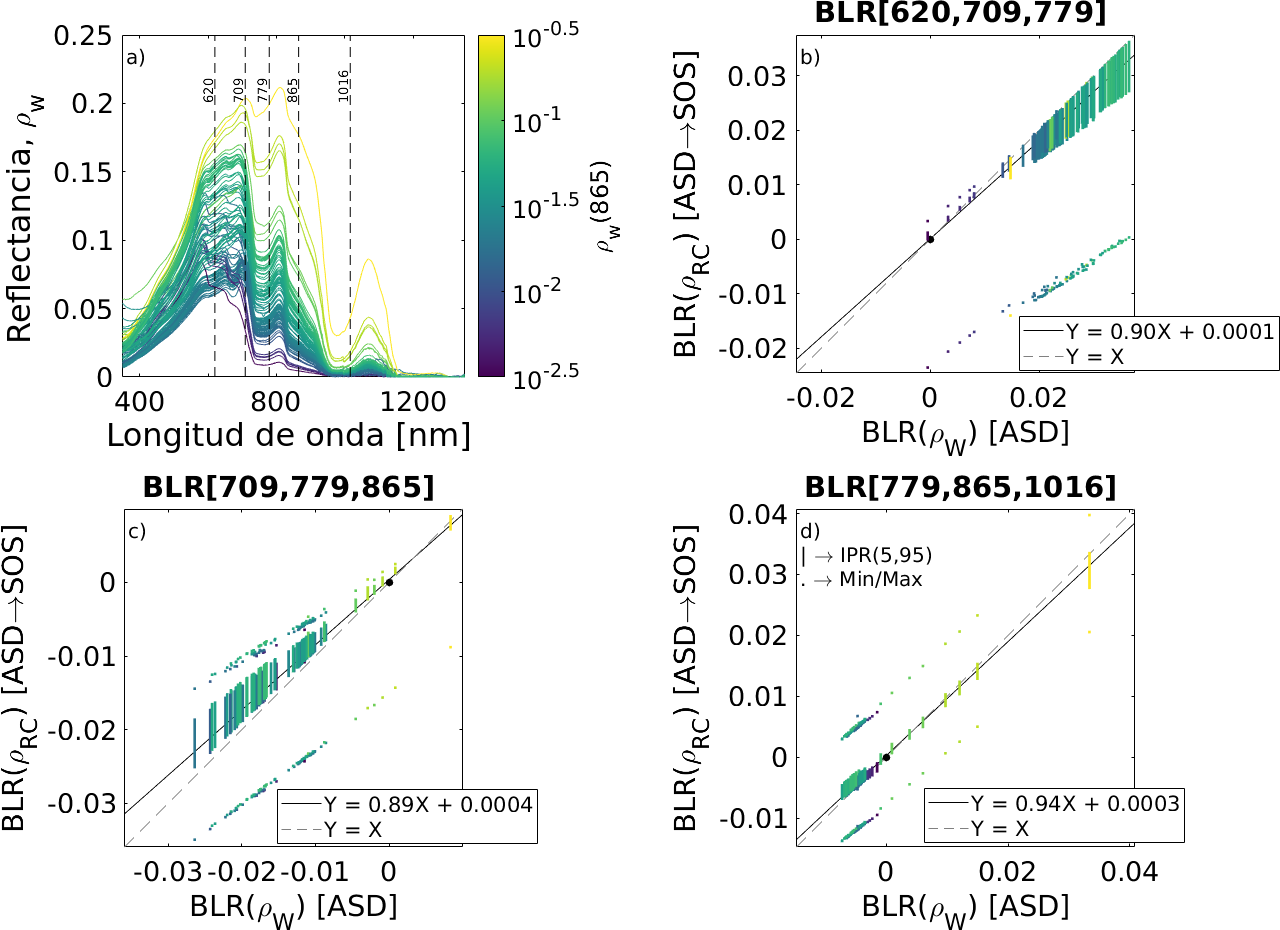
\includegraphics[width=\textwidth]{blr/figures/blrRcSosVsblrWAsd}
        \caption[Comparación entre BLRs de reflectancias del agua medidas y de reflectancias RC simuladas]{a) Reflectancias hiperespectrales obtenidas mediante mediciones radiométricas \textit{in situ} (\S \ref{blr:s:insitu}), utilizadas como reflectancias del agua de entrada en el código de transferencia radiativa CNES-SOS (\S \ref{blr:s:simulations}). Relación entre $BLR(\rho_{w})$ (de las mediciones \textit{in situ}) y $BLR(\rho_{RC})$ (de mediciones \textit{in situ} y simulaciones) para los tripletes $(620,709,779)$ (b), $(709,779,865)$ (c) y $(779,865,1016)$ (d).}
        \label{blr:blrRcSosVsblrWAsd}
        \end{figure}
        
        En todo el conjunto de simulaciones se observó que la dependencia de $t_{BLR}$ con las condiciones geométricas podría reducirse a una sola variable, el factor geométrico de masa de aire, $\mu$ (Ec. \ref{int:eq:mu}) ya que, a excepción de los escenarios con \textit{sunglint} directo, se observó que el acimut relativo tiene un efecto muy pequeño en $t_{BLR}$. Este hecho está bien ilustrado en la Figura \ref{blr:tramsittance}, donde $t_{BLR}$ y su sesgo se representan frente al factor de masa de aire considerando la siguiente expresión:
        
        \begin{equation}
            BLR(\rho_{RC}) = t_{BLR}(\mu)BLR(\rho_{w}) + sesgo(\mu)
            \label{blr:eq:blrtmufactor}
        \end{equation}
        
        En la Figura \ref{blr:tramsittance}, cada punto representa el resultado de $t_{BLR}$ (recuadros superiores) y su correspondiente sesgo (recuadros inferiores) al haber aplicado una regresión lineal de la forma de la Ec. \ref{blr:eq:blrtmufactor} realizada sobre los diferentes subconjuntos definidos por valores específicos para $\theta_{s}$, $\theta_{v}$ y $\phi$, es decir, para condiciones geométricas específicas. Se puede observar que: i) los sesgos son usualmente menores a $0.001$, por lo que no serán tenidos en cuenta en la corrección general de transmitancia, y ii) la dependencia de $t_{BLR}$ con $\mu$ puede considerarse lineal en el rango $\mu\in[2;4]$. Se observan resultados similares al aumentar los espesores ópticos de aerosoles.

        \begin{figure}
        \centering
        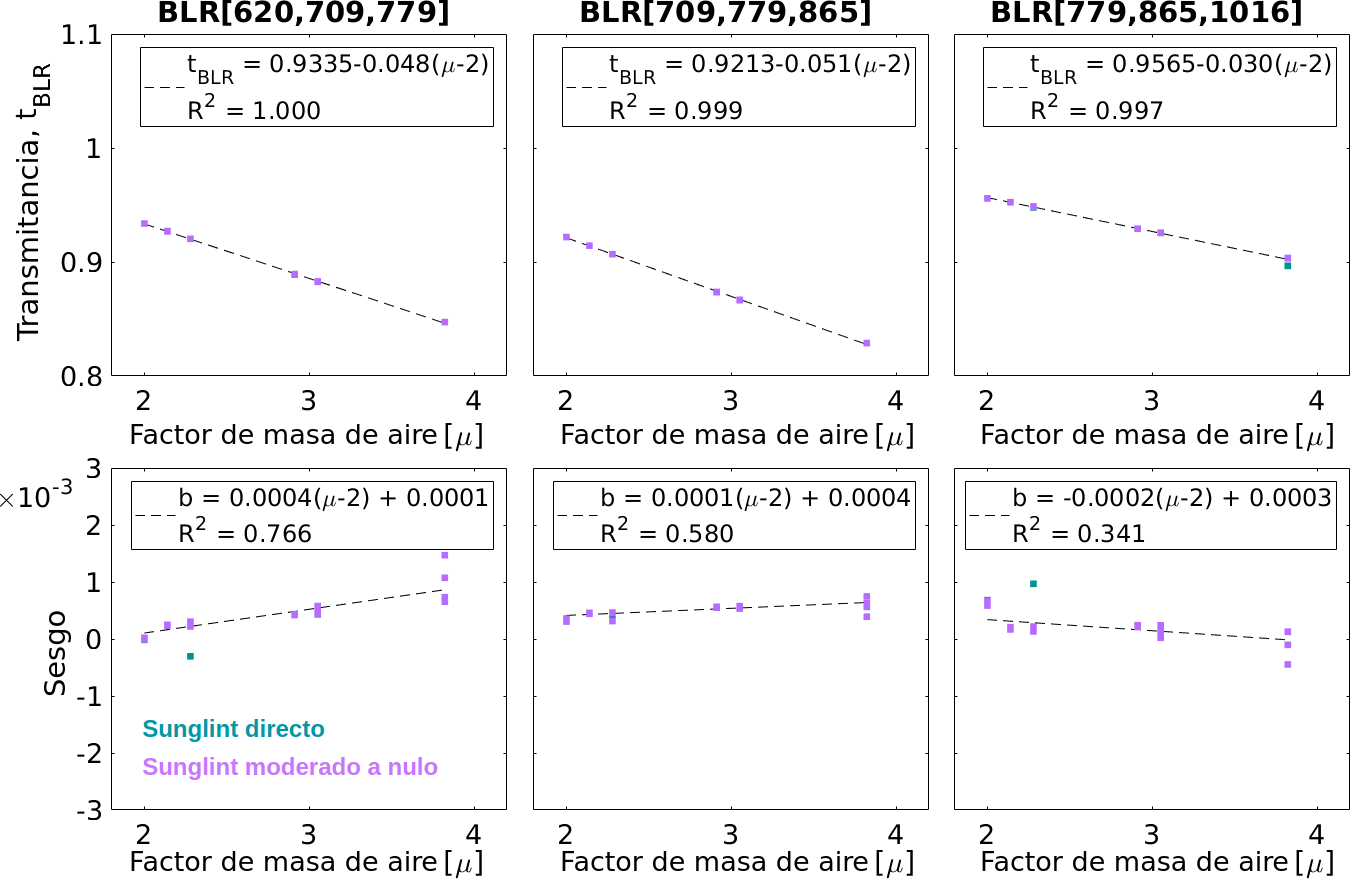
\includegraphics[width=\textwidth]{blr/figures/teqVsMu}
        \caption[Transmitancias equivalentes ($t_{BLR}$) y sesgos vs. factor geométrico de masa de aire para cada BLR utilizado en el esquema BLR-AC.]{Transmitancias equivalentes ($t_{BLR}$, Ecs. \ref{blr:eq:blrtfactor} y \ref{blr:eq:blrtmufactor}) y sesgos vs. factor geométrico de masa de aire, $\mu = \frac{1}{cos(\theta_{s})} + \frac{1}{cos(\theta_{v})}$, para cada BLR utilizado en este trabajo. Los puntos turquesa (violeta) representan los resultados sobre subconjuntos correspondientes a diferentes geometrías de observación/iluminación con (sin) la presencia de \textit{sunglint} directo. Las líneas punteadas indican las regresiones lineales.}
        \label{blr:tramsittance}
        \end{figure}
        
        Sobre la base de estos resultados, los BLRs calculados sobre de escenas RC OLCI utilizadas para estimar la señal del agua son divididos por los factores de transmitancia equivalentes correspondientes para cada píxel (Figura \ref{blr:tramsittance}), para así poder estimar los BLRs asociados a la señal de agua en escenas OLCI, es decir:

        \begin{equation}
            BLR(\rho_{w,OLCI}) := \frac{BLR(\rho_{RC,OLCI})}{t_{BLR}(\mu)}
            \label{blr:eq:blrtolcifactor}
        \end{equation}
        
    \subsection{Relación entre los BLRs y las reflectancias del agua}
    \label{blr:s:blrrhow}

        Las secciones anteriores de este capítulo describieron por qué $BLR(\rho_{w})(620,709,779)$, $BLR(\rho_{w})(709,779,865)$ y $BLR(\rho_{w})(779,865,1016)$ (Ecs. \ref{blr:eq:blr}, \ref{blr:eq:blrrcdepw} y \ref{blr:eq:blrtfactor}) representan un conjunto conveniente de cantidades para estimar la reflectancia del agua en cualesquiera de las bandas consideradas. En este capítulo, nos centramos en establecer una relación entre los BLRs y las reflectancias del agua en al menos dos bandas: 865 nm y 1016 nm, ya que este es el mínimo requerido para eventualmente extrapolar la señal atmosférica a longitudes de onda más cortas (mediante un procedimiento de extrapolación similar al descrito en Gordon y Wang 1994, \cite{gordon1994}).
        Decidimos usar un subconjunto de imágenes OLCI para lograr un conjunto de calibración plausible, a fin de evitar errores sistemáticos que pudieren inducirse al calibrar el algoritmo con datos provenientes de otras fuentes (como mediciones \textit{in situ} o simulaciones de transferencia radiativa).
        Para construir este conjunto de datos, se seleccionó un total de 13 subregiones de 9 imágenes del RdP libres de nubes, \textit{sunglint} o neblina (ver Cuadro \ref{blr:tab:olci}, recuadros magenta en la Figura \ref{blr:Blr14CalValDataSet}). Sobre estas subregiones, se aplicó una CA no operativa para inferir la reflectancia del agua en las bandas de 865 nm y 1016 nm, basándonos en la estimación del componente atmosférico a partir de ventanas de agua clara seleccionadas manualmente - cercanas a las ventanas de interés - de $15 \times 15$ píxeles. Dicha corrección no operativa es denominada en este documento \textit{Fix-AC} (consulte el Cuadro \ref{blr:tab:olci}, recuadros blancos en la Figura \ref{blr:Blr14CalValDataSet}) y supone, para la imagen considerada, un tipo y concentración de aerosoles horizontalmente homogéneos.
        
        \begin{figure}
        \centering
        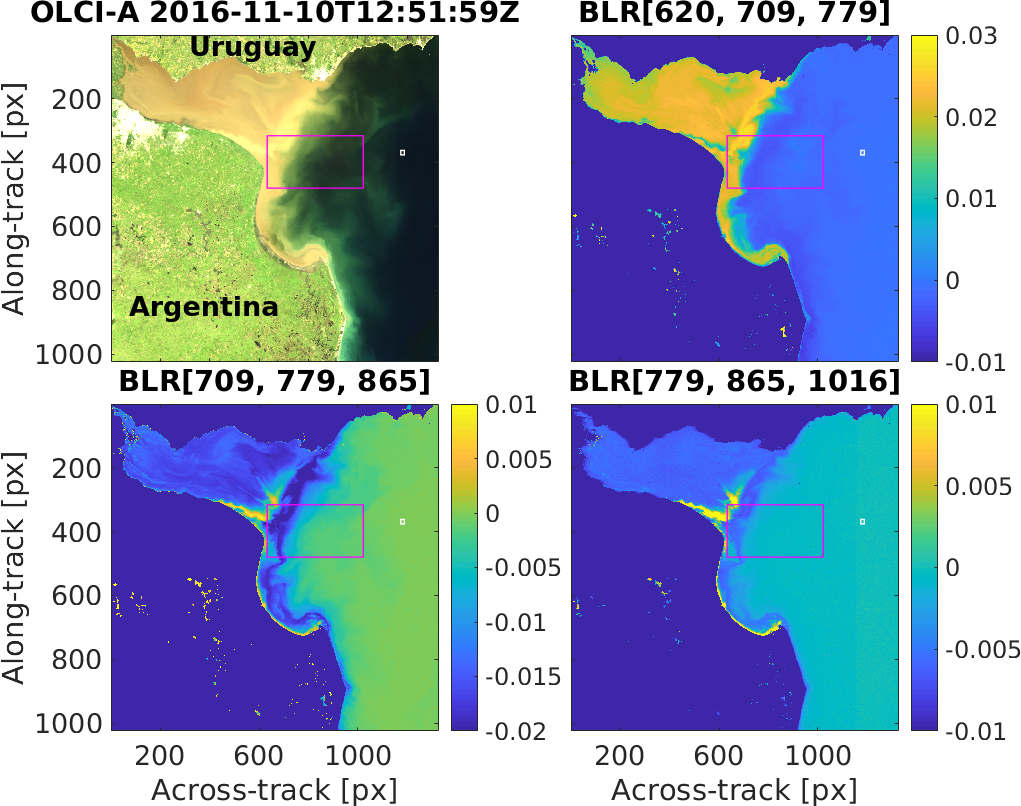
\includegraphics[width=0.8\textwidth]{blr/figures/Blr14CalValDataSet}
        \caption[Ejemplo de una escena que forma parte del conjunto de datos utilizado para calibrar la relación $BLR(\rho_{w})$ vs. $\rho_{w}$.]{Ejemplo de una escena que forma parte del conjunto de datos utilizado para calibrar la relación $BLR(\rho_{w})$ vs. $\rho_{w}$. El cuadro magenta encierra el subconjunto seleccionado de la imagen agregada al conjunto de datos de calibración, mientras que la señal de aerosoles se sustrajo usando el esquema de corrección atmosférica de Ventana Clara Fija (Fix Clear Window, Fix-AC, Ec. \ref{blr:eq:rhow}) de $15 px \times 15 px$, indicadas por los recuadros blancos.}
        \label{blr:Blr14CalValDataSet}
        \end{figure}
        
        Estas \textit{ventanas claras} se eligieron para estar lo más cerca posible de la subregión de interés y a su vez estar totalmente libres de señal de agua en el RNS (determinado por inspección visual de los rásteres $\rho_{RC}$). Esta simple eliminación de aerosol supone una señal atmosférica espacialmente uniforme que se resta de toda la subregión de interés de la siguiente manera:
        
        \begin{equation}
            \rho_{w} = \frac{\rho_{RC} - \rho_{a}^{VentClara}}{t(\lambda)}
            \label{blr:eq:rhow}
        \end{equation}
        
        \noindent donde utilizaremos la expresión simple para el factor de transmitancia difusa dada en la Ec. \ref{int:eq:tDif}, pero en ausencia de aerosoles, $\tau_{a}=0$. Una vez realizado este proceso, el conjunto de datos de calibración formado por las subregiones mencionadas se usa para ajustar una superficie de calibración en el subespacio tridimensional BLR, que es generado por $BLR(620,709,779)$, $BLR(709,779,865)$ y $BLR(779,865,1016)$ (Figuras \ref{blr:Blr14CalValDataSet} y \ref{blr:blr3d}). La superficie de calibración se genera mediante una cuadrícula de malla bidimensional de $X$ - es decir, $BLR(620,709,779)$ - en el rango $(-0.0100;0.0350)$ (paso $0.0005$) e $Y$ - es decir, $BLR(709,779,865)$ - en el rango $(-0.0300;0.0150)$ (paso $0.0005$). Los valores de $Z$ - $BLR(779,865,1016)$ - en cada punto de la cuadrícula se toman como la mediana de los valores $Z$ tomados por el conjunto de datos de calibración en el par $(X,Y)$ correspondiente. Esto se puede hacer de esta manera ya que la superficie BLR no presenta ambigüedad en $Z$, es decir, la superficie BLR puede considerarse como una función de $(X,Y)$: $Z=f(X,Y)$. El punto de calibración se descarta si menos de 10 datos satelitales caen dentro del rango $(X,Y)$ asociado.
        %
        El triplete $BLR(\rho_{w})$ asignado a cada píxel de entrada será el triplete $BLR(\rho_{w})$ más cercano (en el sentido euclidiano) correspondiente a la curva de calibración, junto con la reflectancia del agua en 865 nm y 1016 nm.
        
        \begin{figure}
        \centering
        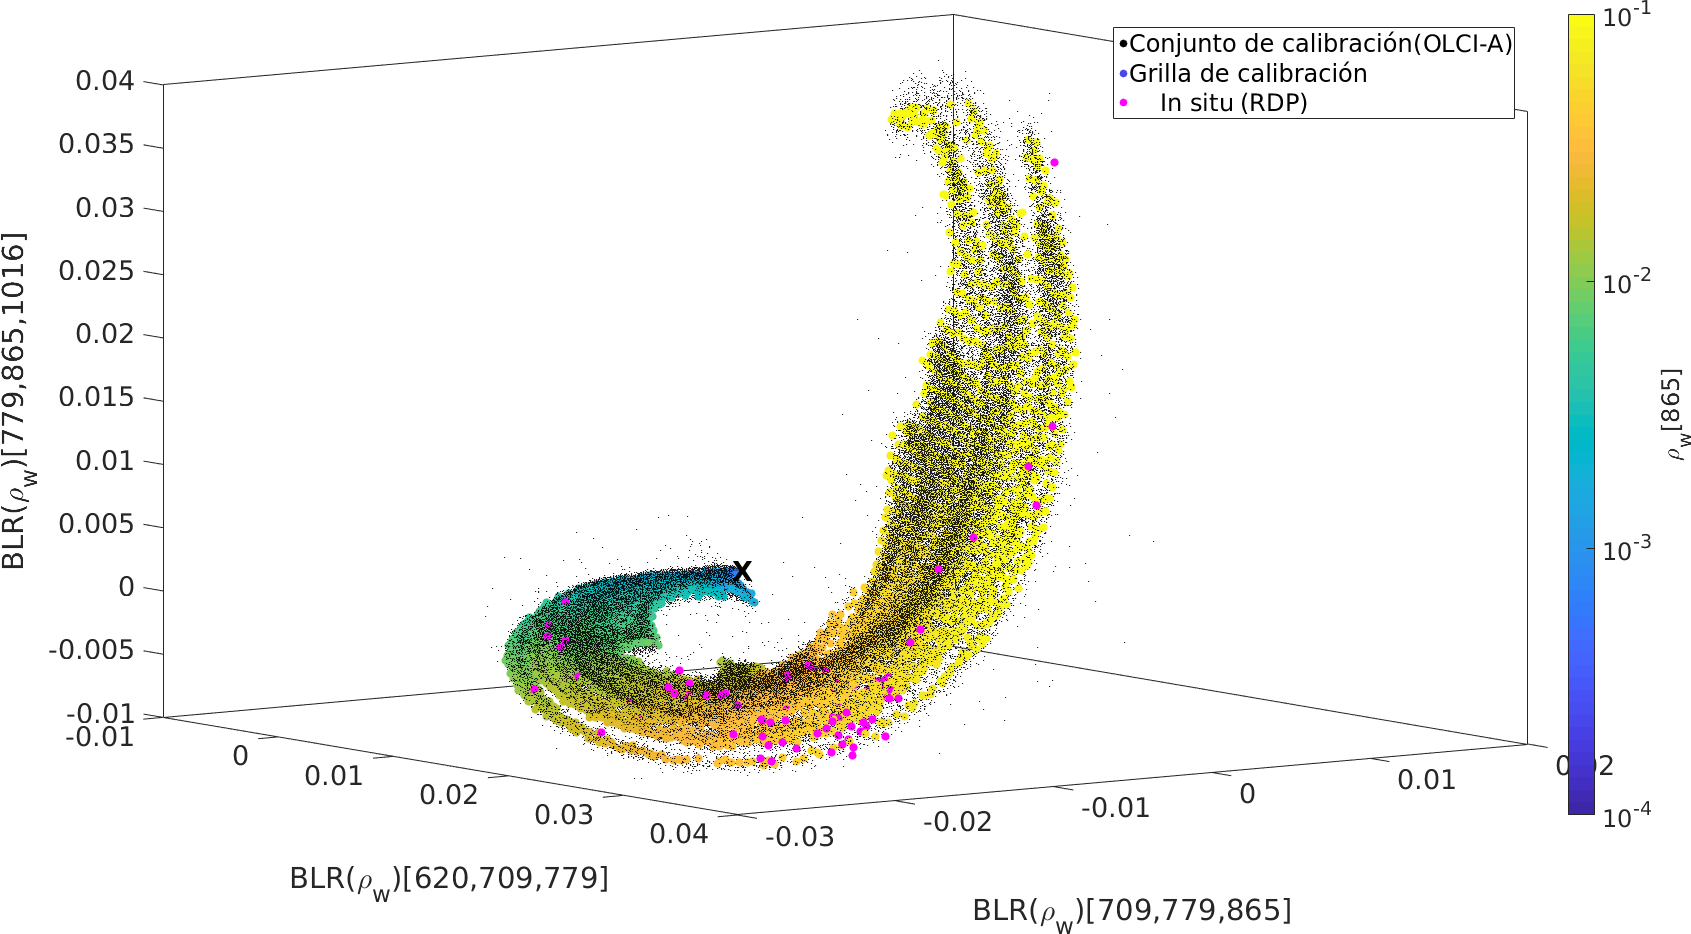
\includegraphics[width=\textwidth]{blr/figures/blr3D}
        \caption[Espacio tridimensional $BLR(\rho_{w})$, formado por los tres BLR linealmente independientes definidos por los tres tripletes consecutivos de las cinco bandas OLCI en 620, 709, 779, 865 y 1016 nm.]{Espacio tridimensional $BLR(\rho_{w})$, formado por los tres BLR linealmente independientes definidos por los tres tripletes consecutivos de las cinco bandas OLCI en 620, 709, 779, 865 y 1016 nm. Puntos pequeños: conjunto de datos de calibración OLCI-A. Puntos grandes mapeados en color: superficie de calibración obtenida del conjunto de datos de calibración OLCI-A, cuyo color indica reflectancia del agua a 865 nm. Los puntos magentas son datos \textit{in situ}. El origen se indica con una X y corresponde a un escenario de \textit{aguas claras}, Ec. \ref{int:eq:blackPixelAmplitud}.}
        \label{blr:blr3d}
        \end{figure}

    \subsection{Elección de bandas}
    \label{blr:s:bandchoice}
    
        En este capítulo, hemos optado por utilizar las reflectancias RC calculadas a partir de las bandas OLCI en 620, 709, 779, 865 y 1016 nm. Estas 5 bandas conforman un espacio $\mathbb{R}^{5}$, del cual consideramos un subespacio conformado por tres BLRs consecutivos, linealmente independientes: $BLR(\rho_{RC})(620, 709, 779)$, $BLR(\rho_{RC})(709, 779, 865)$ y $BLR(\rho_{RC})(779, 865, 1016)$. Estas bandas se han elegido para i) maximizar el impacto de la señal del agua (turbia) en $BLR(\rho_{RC})$, y simultáneamente ii) minimizar el impacto de los componentes atmosféricos. No se consideraron otras bandas OLCI dentro de esta región espectral, por ej. aquellas en el rango de 760-770 nm y la banda centrada a 940 nm, ya que están fuertemente afectadas por la absorción de gases troposféricos (\S \ref{int:s:tAbs}). Las bandas OLCI en el rango de 660-690 nm también se evitan porque las reflectancias del agua pueden verse afectadas por la absorción y la fluorescencia de la clorofila (véase Figura \ref{dat:HyperTriOS}).

    \subsection{Estimación de la reflectancia de aerosoles en las bandas 865 nm y 1016 nm}
    \label{blr:s:residual}

        La reflectancia de aerosoles, $\rho_{a}$, en 865 nm y 1016 nm es computada para testear el grado de correlación espacial con la reflectancia del agua estimada - que se espera sea baja - utilizando la siguiente expresión simplificada:
        
        \begin{equation}
            \rho_{a}(\lambda) = \rho_{RC}(\lambda) - t(\lambda,\mu)\rho_{w,j}(\lambda)
            \label{blr:eq:residual}
        \end{equation}
        
        \noindent donde $\rho_{w,j}$ es el valor de reflectancia del agua asignado al vecino euclidiano más cercano desde la superficie de calibración en el espacio BLR.
        El factor de transmitancia difusa se calculó también utilizando la Ec. \ref{int:eq:tDif} a $\tau_{a}=0$. Esta misma expresión se aplicó para intercomparar con las reflectancias en aerosol producidas por otros esquemas preexistentes (BAC/BPAC y SeaDAS-2(865,1016)).
        Se realiza una última corrección en $\rho_{a}(865)$ para restringir el valor se $\epsilon_{a}(865,1016)=\frac{\rho_{a}(865)}{\rho_{a}(1016)}$ dentro del rango de $(0.85; 1.25)$. Estos límites se determinaron como los valores extremos tomados en un conjunto de 82 ventanas diferentes de tamaño $15px \times 15px$ de escenas OLCI-A de regiones de aguas claras cerca del Río de la Plata, Bahía Blanca, Mar del Norte, Mar Amarillo, Amazonas y el norte de Australia. Además, estos límites son consistentes con lo que se obtuvo sobre las simulaciones CNES-SOS. Esta corrección se realiza imponiendo la siguiente condición píxel a píxel:
        
        \begin{equation}
            0.85\rho_{a}(1016) \leq \rho_{a,new}(865) \leq 1.25\rho_{a}(1016)
            \label{blr:eq:epsCorr}
        \end{equation}

        y luego, corrigiendo consecuentemente los valores de $\rho_{w}(865)$ obtenidos. Esta restricción asume como más confiables los valores estimados de $\rho_{w}(1016)$ por sobre los de $\rho_{w}(865)$ cuando el $\epsilon_{a}(865,1016)$ estimado cae fuera del rango esperado de variabilidad natural y se discute más en la \S \ref{blr:s:discussion}.

    \subsection{Esquema de corrección atmosférica: resumen}
    \label{blr:s:summary}

    La siguiente enumeración resume el algoritmo de CA desarrollado en el presente capítulo:
    
    \begin{enumerate}
        \item La corrección por EPVs (\S \ref{ppe}) se aplica en las imágenes L1B (radiancias a TOA).
        \item La corrección por Rayleigh (y absorción gaseosa) se aplica utilizando el software SeaDAS v7.5.
        \item Se calculan $BLR(\rho_{RC})(620,709,779)$, $BLR(\rho_{RC})(709,779,865)$ y $BLR(\rho_{RC})(779,$ $865,1016)$ a partir de las correspondientes reflectancias corregidas por Rayleigh (ver \S \ref{blr:s:atb} - \ref{blr:s:bandchoice}, Ec. \ref{blr:eq:blr}).
        \item Se aplica una corrección del factor de transmitancia para relacionar $BLR(\rho_{RC})$ con $BLR(\rho_{w})$ (véase \S \ref{blr:s:transmittance}, Ec. \ref{blr:eq:blrtolcifactor})
        \item Para cada píxel, los BLRs calculados se asocian al triplete de BLRs desde la superficie de calibración que minimizan la distancia euclidiana en el espacio BLR. Se asigna al píxel en cuestión la reflectancia del agua correspondiente a 865 nm y 1016 nm (\S \ref{blr:s:blrrhow}).
        \item La señal atmosférica en estas bandas se obtiene restando la señal de agua asignada (habiéndole aplicado un factor de transmitancia difusa) a la reflectancia RC (\S \ref{blr:s:residual}, Ec. \ref{blr:eq:residual}).
        \item Se aplica una restricción final a $\rho_{a}(865)$ para limitar $\epsilon_{a}(865,1016)$ dentro del rango razonable de $(0.85; 1.25)$ (\S \ref{blr:s:residual}, Ec. \ref{blr:eq:epsCorr}).
    \end{enumerate}
    
    % \begin{figure}
    % \centering
    % 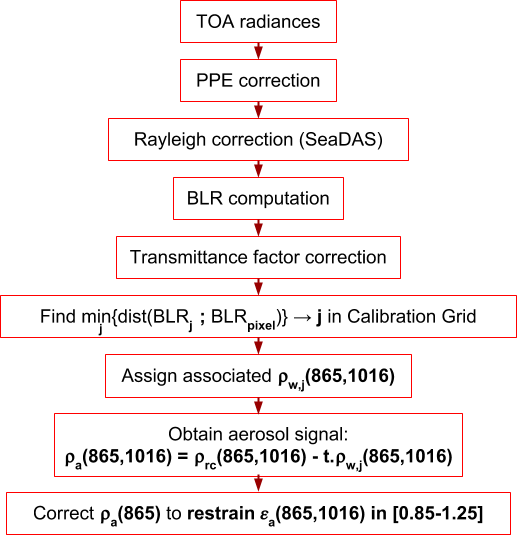
\includegraphics[width=7 cm]{blr/figures/blrScheme}
    % \caption{Esquema de corrección atmosférica por BLR (BLR-AC), detallado en el resumen.}
    % \label{blr:scheme}
    % \end{figure}
    
    Este abordaje puede extenderse a todo el rango de bandas de interés restando la reflectancia del agua estimada en el NIR a la reflectancia a TOA (con la adecuada aplicación del factor de transmitancia difusa) y aplicando la suposición de píxeles claros para extrapolar la señal de aerosoles a longitudes de onda más cortas (Gordon y Wang 1994, \cite{gordon1994}, Stumpf et al. 2003, \cite{stumpf2003}).
    
    \subsection{Efecto del ruido del sensor sobre los BLRs}
    \label{blr:s:blrNoise}

        \subsubsection{Cómputo del ruido absoluto del sensor}
        \label{blr:s:blrNoiseHA}
            Para analizar el alcance del ruido sobre las bandas OLCI involucradas en el cómputo de los BLRs, se estimó el error asociado al ruido del sensor para todas las bandas utilizadas. Para ello, se utilizaron 82 ventanas de $15 px \times 15 px$ de imágenes L2 de reflectancias corregidas por Rayleigh (habiendo utilizado SeaDAS al igual que en \S \ref{blr:s:olci}) cercanas al RdP en condiciones de cielo despejado y aguas claras, lo cual equivaldría en el RNS a condiciones de baja variabilidad espacial dentro de las ventanas. De esta forma, es posible aplicar el método de \textit{Área Homogénea} propuesto por Duggin et al. 1985, \cite{duggin1985}. Dicho método consiste en asociar el desvío estándar sobre dichas ventanas al ruido en la imagen, de forma tal de que
            
            \begin{equation}
                \sigma(\rho_{RC}(\lambda_{i})) = \frac{1}{N}\sum_{j=1}^{N} \sigma(\rho_{RC}^{j}(\lambda_{i}))
                \label{blr:eq:noiseHA}
            \end{equation}
            
            \noindent
            corresponda al valor absoluto del ruido sobre la reflectancia RC estimado para la banda centrada en $\lambda_{i}$ (aquí $\sigma(\cdot)$ representa el desvío estándar). En esta ecuación, $\rho_{RC}^{j}(\lambda_{i})$ es el ráster de la reflectancia RC de la banda $\lambda_{i}$ para la $j$-ésima ventana de 
            $15 px \times 15 px$ considerada, $N$ es el número de imágenes consideradas y $std(\cdot)$ es el desvío estándar.
            
            A partir de este análisis se obtuvieron los valores de ruido absoluto reportados en el Cuadro \ref{blr:tab:blrNoise} para las bandas 620, 709, 779, 865 y 1016 nm. Dichos valores fueron luego utilizados para estimar la propagación del ruido del sensor sobre los BLRs.
            %
            En este procedimiento utilizaremos el ruido absoluto y no la relación señal-ruido (SNR) dado que esta última siempre es referida a un valor de radiancia/reflectancia típico, valor que \textit{a priori} se desconoce o bien está referido a aguas claras.
            
            \begin{table}
            \caption{Valores absolutos del ruido sobre las reflectancia RC de las bandas 620, 709, 779, 865 y 1016 nm de OLCI-A obtenidos mediante el método de \textit{Área Homogénea}.}
            \begin{tabular}{|l|l|l|l|l|l|}
            \hline
            \textbf{Banda}, $[nm]$            & \textbf{620} & \textbf{709} & \textbf{779} & \textbf{865} & \textbf{1016} \\ \hline
            \textbf{Ruido}, $\sigma[10^{-4}]$ & 5.610        & 4.868        & 4.925        &  4.812       &  8.059        \\ \hline
            \end{tabular}
            \label{blr:tab:blrNoise}
            \end{table}

        \subsubsection{Propagación del ruido del sensor sobre los BLRs}
        \label{blr:s:blrNoiseBLR}
            
            Tal como lo expuesto por Curran et al. 1989, \cite{curran1989}, o por Gross et al. 2007, \cite{gross2007}, podremos asumir que el ruido del sensor es independiente de la señal natural y lo consideramos como una variable aleatoria normal aditiva, es decir:
            
            \begin{equation}
                \rho_{RC}(\lambda_{i}) \rightarrow \rho_{RC}(\lambda_{i}) + \varepsilon(\lambda_{i}) =  \rho_{RC}(\lambda_{i}) + \mathcal{N}(0,\sigma_{i})
                \label{blr:eq:rhoRCNoise}
            \end{equation}

            \noindent siendo $\mathcal{N}(0,\sigma_{i})$ una variable aleatoria de distribución normal de media $0$ y desvío estándar $\sigma_{i}$. Para entender cómo se propaga el ruido del sensor en el cálculo de los BLRs, observemos que las Ecs. \ref{blr:eq:blr} y \ref{blr:eq:baseline} pueden ser rescritas como combinación lineal de las reflectancias dentro del triplete considerado:
            
            \begin{equation}
                BLR(\rho_{RC})[\lambda_{L},\lambda_{M},\lambda_{R}] = \sum_{i=L,M,R} A_{i}\rho_{RC}(\lambda_{i}) \rightarrow \sum_{i=L,M,R} A_{i}\rho_{RC}(\lambda_{i}) + \varepsilon(\lambda_{i})
                \label{blr:eq:blrCL}
            \end{equation}

            \noindent
            donde las $A_{i}$ son constantes que dependen únicamente de las longitudes de onda de las bandas de cada triplete y se reportan en el Cuadro \ref{blr:tab:blrCoef}.

            \begin{table}
            \caption{Coeficientes que acompañan a las reflectancias RC en el cálculo de los BLRs (Ec. \ref{blr:eq:blrCL}).}
            \begin{tabular}{|l|l|l|l|}
            \hline
            \textbf{Bandas/Coeficientes}    & \textbf{$A_{L}$} & \textbf{$A_{M}$} & \textbf{$A_{R}$} \\ \hline
            \textbf{$BLR(\rho)[620,709,779] $} & -0.440252               & 1                       & -0.559748               \\ \hline
            \textbf{$BLR(\rho)[709,779,865] $} & -0.551282               & 1                       & -0.448718               \\ \hline
            \textbf{$BLR(\rho)[779,865,1016]$} & -0.637131               & 1                       & -0.362869               \\ \hline
            \end{tabular}
            \label{blr:tab:blrCoef}
            \end{table}

            \noindent
            entonces es válido considerar que cada BLR será a su vez una variable aleatoria de distribución normal cuyo desvío estándar se expresa de la siguiente manera.

            \begin{equation}
                \sigma_{BLR}^{2} = \sum_{i=L,M,R}A_{i}^{2}\sigma_{i}^{2}
                \label{blr:eq:blrNoiseCL}
            \end{equation}
            
            Considerando esta expresión y el hecho de que los valores de $A_{i}$ son menores a la unidad para las bandas laterales ($i=L$ e $i=R$), se desprende que el aporte del ruido del sensor en las bandas laterales será comparativamente menor al de la banda central ($i=M$). Por ejemplo, dado que $A_{1016} = -0.362869$ en el cálculo de $BLR(\rho_{RC})[779,865,1016]$, el aporte del ruido de la banda de 1016 nm a este BLR - la banda con ruido más elevado dentro del conjunto considerado - será de $\approx 13 \%$ del ruido original de dicha banda.

%%%%%%%%%%%%%%%%%%%%%%%%%%%%%%%%%%%%%%%%%%
\section{Resultados}
\label{blr:s:results}

    \subsection{BLRs en aguas claras y turbias}
    \label{blr:s:results:blrs}

        El hecho de que los BLRs considerados en la región espectral RNS se acercan a valores cercanos a cero en aguas claras es consistente con lo expresado en la Ec. \ref{blr:eq:blrrcdepw}, suponiendo que las aguas muy claras son en realidad negras en el RNS para un sensor remoto óptico. Esta propiedad se ve claramente a partir de las reflectancias RC de OLCI, y es evidente en la Figura \ref{blr:blrHist} (así como en las Figuras \ref{blr:blrExamples} y \ref{blr:Blr14CalValDataSet}), donde se intercomparan las distribuciones de BLRs provenientes de i) ventanas seleccionadas para realizar la calibración BLR-AC (que contienen principalmente aguas turbias, \textit{ventanas de calibración} en el Cuadro \ref{blr:tab:olci}), y ii) ventanas seleccionadas para realizar el esquema Fix-AC (que contienen aguas muy claras, \textit{ventanas Fix-AC} en el Cuadro \ref{blr:tab:olci}). En la Figura \ref{blr:blrHist} se observa que los valores medios de BLR y los rangos intercuartiles (IQR) sobre las ventanas Fix-AC se aproximan a 0 (siempre menores que $10^{-3}$) y que los IQRs estimados en dichas ventanas son al menos 9 veces más pequeños que los IQRs calculados para las ventanas de calibración.
        Esto es consistente con lo que se ha predicho y muestra que para este enfoque, el supuesto de agua negra se traduce a la condición $BLR(\rho_{w})=0$ (también evidente al observar las regiones de agua clara en la Figura \ref{blr:Blr14CalValDataSet}). Esto significa que, dado un píxel donde simultáneamente $BLR(\rho_{w})=0$ para los tres tripletes considerados, el algoritmo estima $\rho_{w}(865)=\rho_{w}(1016)=0 $, es decir, el algoritmo vuelve naturalmente al enfoque estándar de CA para aguas claras.
        
        \begin{figure}
        \centering
        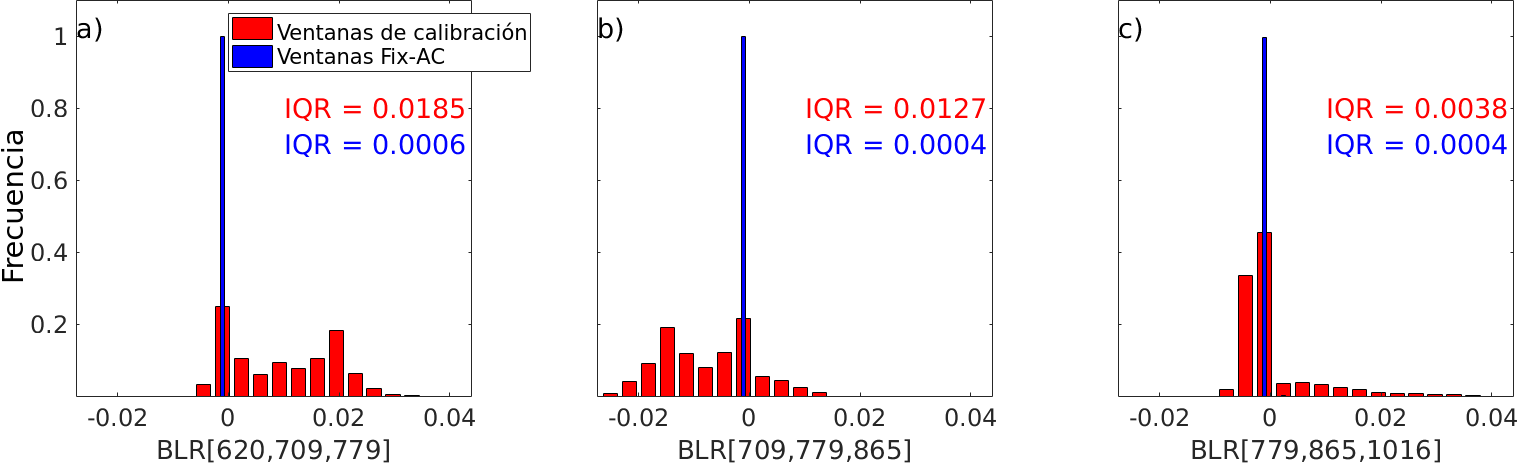
\includegraphics[width=\textwidth]{blr/figures/blrHistClearVsTurbid}
        \caption[Histogramas de $BLR(\rho_{w})$ en los tripletes $(620,709,779)$ nm (a), $(709,779,865)$ nm (b) y $(779,865,1016)$ nm (c) para el conjunto completo de ventanas de calibración y para las ventanas de aguas claras.]{Histogramas de $BLR(\rho_{w})$ en los tripletes $(620,709,779)$ nm (a), $(709,779,865)$ nm (b) y $(779,865,1016)$ nm (c) para: el conjunto completo de ventanas de calibración (en rojo, Cuadro \ref{blr:tab:olci}) y para las ventanas de aguas claras (en azul, ventanas Fix-AC en el Cuadro \ref{blr:tab:olci}), mostrando que los BLRs se aproximan a 0 en aguas claras.}
        \label{blr:blrHist}
        \end{figure}
        
        Esto también es evidente en la Figura \ref{blr:blrVsRho}, donde se intercompara la relación $BLR$ vs. $\rho_{w}$ proveniente de tres fuentes diferentes de información para mostrar cómo los BLRs en cada uno de los tres tripletes de longitudes de onda considerados varían según las reflectancias del agua a 865 nm y 1016 nm. Los puntos azules muestran datos de las ventanas de calibración (Cuadro \ref{blr:tab:olci}); en magenta, los BLRs calculados a partir de los datos \textit{in situ} recopilados del Río de la Plata (\S \ref{blr:s:insitu}), y una familia de curvas de colores muestran la relación $BLR$ vs. $\rho_{w}$ usando un modelo de reflectancia basado en la Aproximación de Dispersión cuasi-Simple (quasi-Single Scattering Albedo, qSSA), descrito en \S \ref{qssa}. Esta familia de curvas fue construida asumiendo que en las bandas del RNS consideradas la única componente bioóptica influyente en aguas turbias del RdP es el material particulado en suspensión. Para estas curvas se fijaron los coeficientes de dispersión y absorción específicos de partículas (descritos en \S \ref{qssa:s:iops_spm}), a excepción del parámetro de absorción de partículas a 443 nm que se varió en el rango $[0.021-0.062]g/m^{2}$ y donde el material particulado en suspensión (SPM) varió logarítmicamente entre $0.001 g/m^{3}$ y $10000 g/m^{3}$.

        \begin{figure}
        \centering
        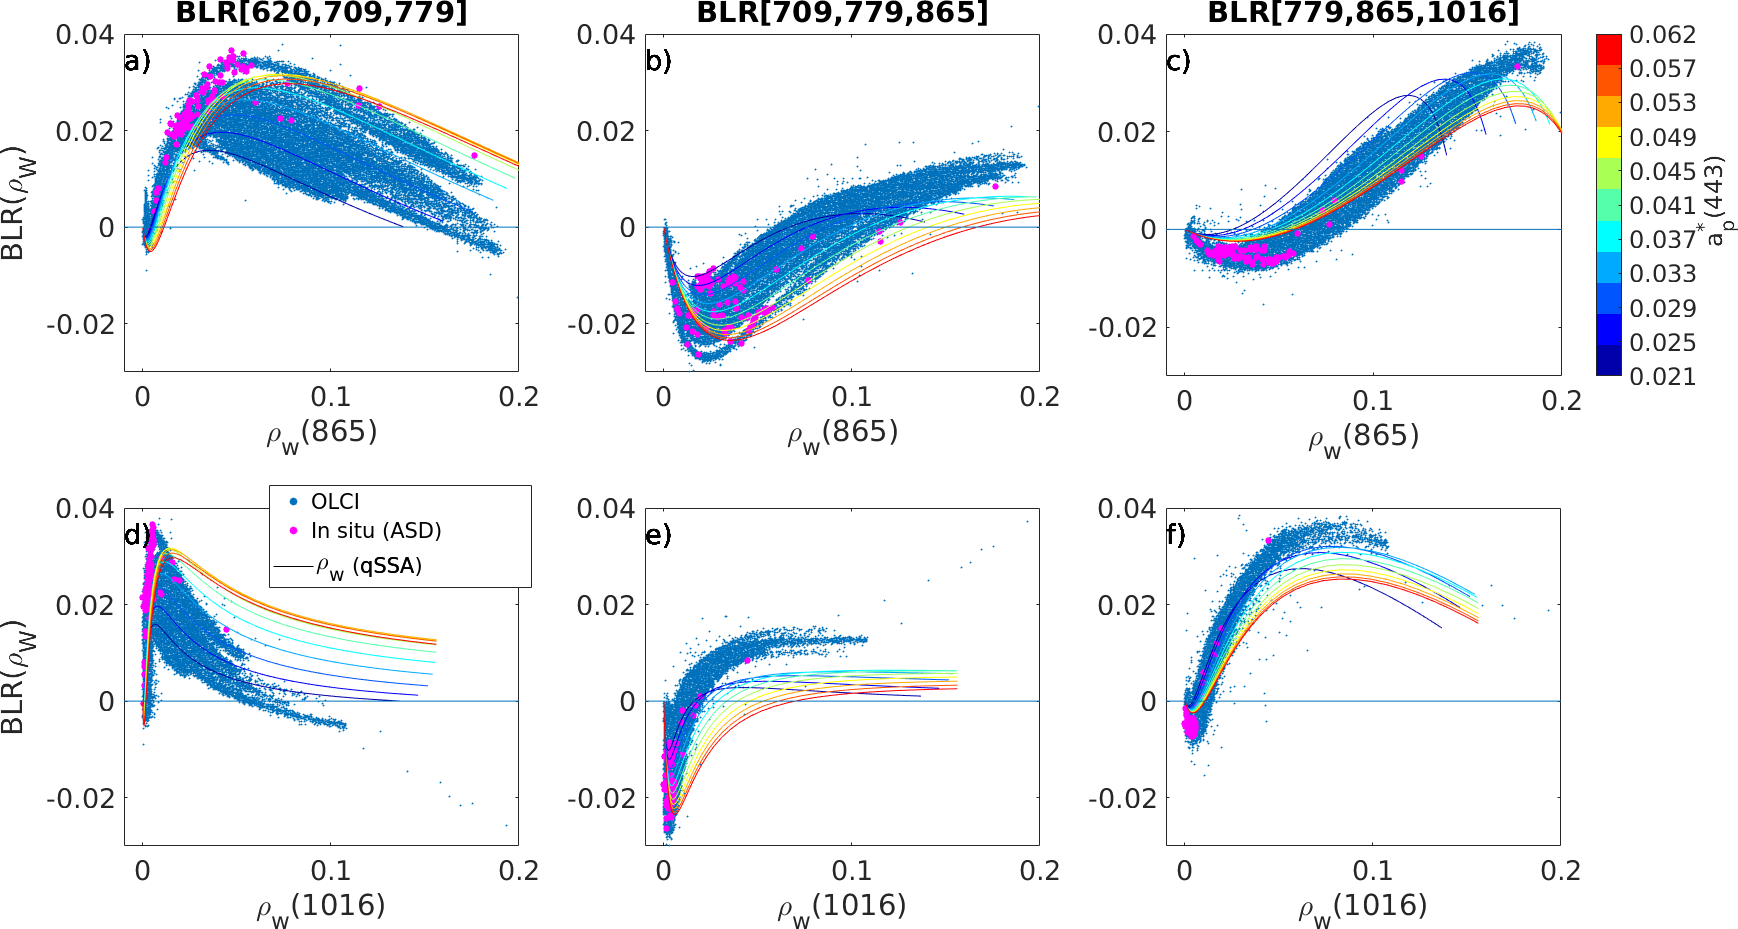
\includegraphics[width=\textwidth]{blr/figures/blrVsrhoWCalDSqSSAinSitu}
        \caption[$BLR(\rho_{w})$ en los tripletes $(620,709,779)$, $(709,779,865)$ y $(779,865,1016)$ vs. reflectancia del agua, $\rho_{w}$, en las bandas 865 nm (a-c) y 1016 nm (d-f).]{$BLR(\rho_{w})$ en los tripletes $(620,709,779)$, $(709,779,865)$ y $(779,865,1016)$ vs. reflectancia del agua, $\rho_{w}$, en las bandas 865 nm (a-c) y 1016 nm (d-f). En azul se grafican los datos extraídos de OLCI de diversas imágenes. Los puntos en magenta corresponden a mediciones radiométricas \textit{in situ}. Las líneas coloreadas corresponden a diferentes reflectancias brindadas por el modelo de Aproximación de Dispersión cuasi-Simple (qSSA, \S \ref{qssa}).}
        \label{blr:blrVsRho}
        \end{figure}
        
        Si bien existe una semejanza evidente entre las tres fuentes de información, debe notarse que las curvas qSSA se apartan de los datos medidos (tanto remótamente como \textit{in situ}) principalmente debido a que el modelo de reflectancia analítica utilizado es menos confiable a reflectancias altas debido al fuerte efecto de la dispersión múltiple a altas concentraciones de partículas.
        Las variaciones sobre la relación BLR vs. $\rho_{w}$ observadas entre las diferentes curvas qSSA indican que los BLRs pueden ser muy sensibles a la absorción de partículas; lo que significa que podrían usarse como indicativos de diferentes propiedades ópticas específicas de partículas en aguas muy turbias. No obstante, esta hipótesis debe verificarse simultáneamente con mediciones radiométricas y con datos de campo de absorción de partículas.
        
        En los tres tripletes considerados, el modelo $BLR(\rho_{w})$ se comporta de manera similar al aumentar la reflectancia. En $\rho_{w}=0$, todos se acercan a los valores cercanos a 0, recuperando el supuesto de agua negra $BLR(\rho_{w}=0)=0$ visto en la Figura \ref{blr:blrHist}. A medida que aumentan las reflectancias, los BLRs toman valores negativos, lo que se puede entender si consideramos $\rho_{w} \propto \frac{b_{b,p}^{*}}{a_{w}}$ para turbideces muy bajas (bajo contenido de sedimento) (cf. Ruddick et al. 2006, Ec. 14 \cite{ruddick2006}). Dado el modelo simple de reflectancia qSSA descrito en \S \ref{qssa}, con IOPs específicas tomadas de los valores informados en Babin et al. 2003 (a y b),\cite{babin2003a}\cite{babin2003b}, esta magnitud es convexa para las bandas OLCI consideradas, es decir, BLRs negativos (Figura \ref{blr:blrBehaviorLimits} a).
        Por el contrario, para turbideces muy altas, las reflectancias del agua tienden a alcanzar un valor constante (saturación) que depende de las IOPs específicas del contenido de partículas del agua: $\rho_{w} \propto \frac{b_{b,p}^{*}}{a_{p}^{*}+b_{b,p}^{*}}$ (cf. Dogliotti et al. 2015, Ec. A2, \cite{dogliotti2015}). En este caso, esta magnitud es cóncava para las bandas OLCI consideradas en el modelo de relfectancia qSSA, es decir, BLRs positivos (Figura \ref{blr:blrBehaviorLimits}b).
        
        \begin{figure}
        \centering
        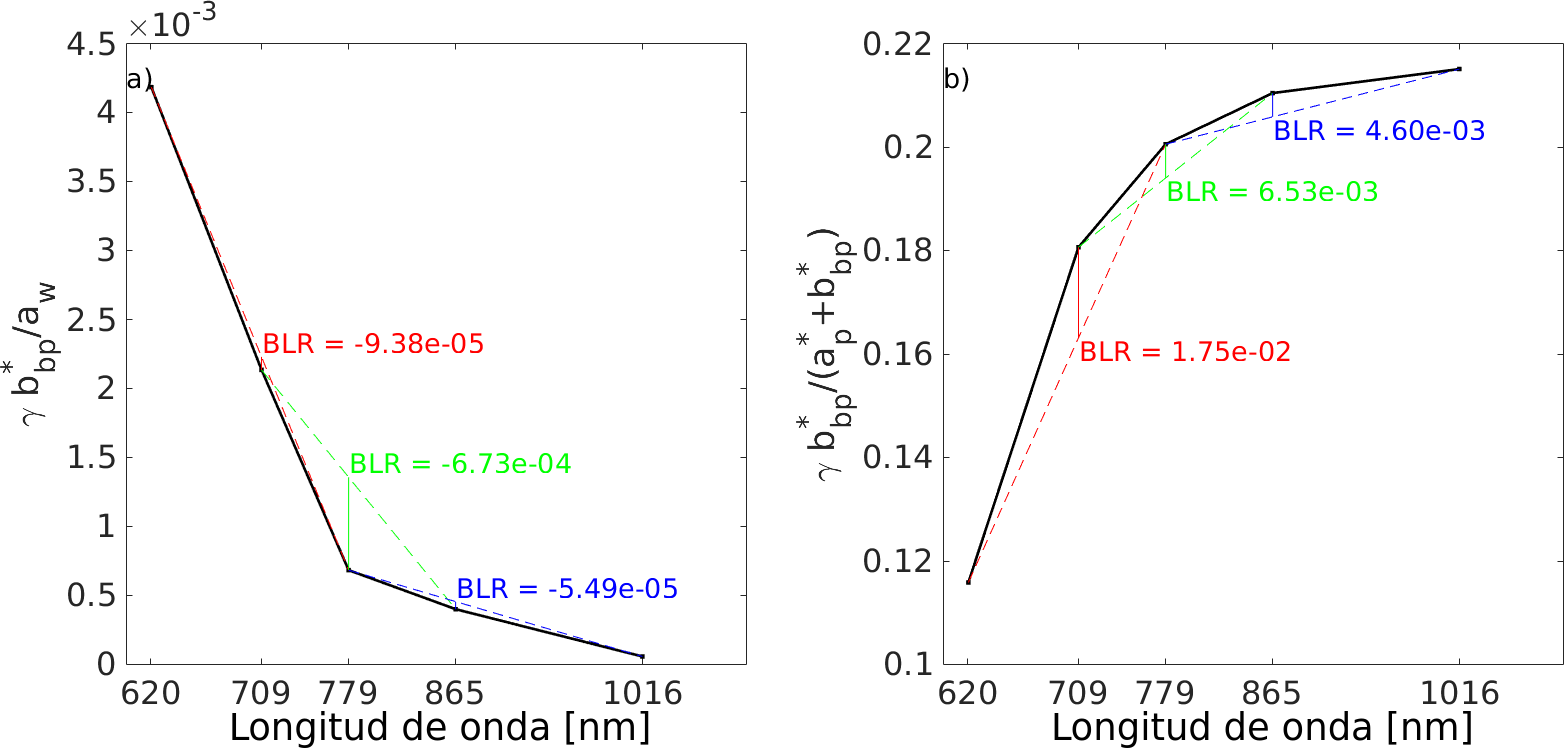
\includegraphics[width=\textwidth]{blr/figures/blrBehaviorLimits}
        \caption{Reflectancias del agua teóricas en las bandas de los BLRs otorgadas por el modelo de Aproximación de Dispersión cuasi-Simple (qSSA) a muy baja (a) y muy alta (b) concentración de partículas.}
        \label{blr:blrBehaviorLimits}
        \end{figure}

    \subsection{Efecto del ruido del sensor sobre los BLRs}
    \label{blr:s:results:blrNoise}    
        
        La Figura \ref{blr:blrQssaNoise} muestra una estimación teórica del rango de variación provocado por el ruido del sensor sobre los BLRs. Para dicha estimación se aplicaron: i) el modelo de reflectancia basado en la aproximación de Dispersión cuasi-Simple descrito en la \S \ref{qssa}; ii) los valores de error absoluto calculados mediante la aproximación de Área Homogénea, descrita en la \S \ref{blr:s:blrNoiseHA}, y la Ec. \ref{blr:eq:blrNoiseCL}.
        
            \begin{figure}
            \centering
            \includegraphics[width=0.7\textwidth]{blr/figures/blrQssaNoise}
            \caption[Efecto del ruido sobre los BLRs, calculado a partir del método de Área Homogénea y del modelos qSSA de reflectancia del agua.]{Valores de los BLRs considerados en este capítulo teniendo en cuenta el modelo de reflectancia del agua basado en la Aproximación de Dispersión cuasi-Simple (curvas sólidas), junto con los valores del desvío estándar del modelo teórico de error calculado a partir de la Ec. \ref{blr:eq:blrNoiseCL}.}
            \label{blr:blrQssaNoise}
            \end{figure}

        La Figura \ref{blr:blrQssaNoise} nos muestra que el efecto del ruido del sensor sobre los BLRs es suficientemente chico como para afirmar que, dadas las características del sensor considerado - OLCI-A - el mismo será capaz de resolver la forma funcional dada por la varibilidad natural de los BLRs estudiados por sobre el ruido del sensor.
        Por otro lado, la Figura \ref{blr:blrRhoRC1016Noise} muestra la reflectancia RC a 1016 nm y el $BLR(\rho_{RC})(779,865,1016)$ de una imagen OLCI-A del RdP (17 de agosto de 2016), donde se observa que el ruido de la banda a 1016 nm tiene un bajo impacto en el BLR, tal como fue detallado en la \S \ref{blr:s:blrNoise}. Más allá de estos resultados consideramos que es necesario realizar un análisis más exhaustivo del efecto del ruido del sensor sobre el desempeño de la CA.
    
        \begin{figure}
        \centering
        \includegraphics[width=\textwidth]{blr/figures/blrRhoRC1016Noise.png}
        \caption{Reflectancia RC a 1016 nm, $\rho_{RC}(1016)$ (a) y $BLR(\rho_{RC})[779,865,1016]$ (b) correspondientes al sensor OLCI-A sobre el Río de la Plata del día 17 de agosto de 2016.}
        \label{blr:blrRhoRC1016Noise}
        \end{figure}

    \subsection{Desempeño de la corrección atmosférica}
    \label{blr:s:results:blrac}

        \subsection{Validación con datos \textit{in situ} (\textit{match-ups})}
        \label{blr:s:results:blrac:matchups}

            Las Figuras \ref{blr:matchups_rho_hyper}, \ref{blr:matchups_rho_scatter}, \ref{blr:matchups_rho_MAE} y \ref{blr:matchups_T} muestran los resultados obtenidos para el ejercicio de \textit{match-up} realizado sobre las mediciones de las estaciones del Cuadro \ref{blr:tab:matchups} (Dogliotti y Gossn 2019, \cite{dogliottiGossn2019}). La Figura \ref{blr:matchups_rho_hyper} muestra las reflectancias del agua medidas \textit{in situ} (líneas sólidas) y los valores de reflectancia del agua obtenidos al aplicar diferentes CAs entre las que se halla la propuesta en este capítulo (denominada con el acrónimo BLR-AC). Cabe resaltar que en este ejercicio de intercomparación se consideraron únicamente bandas en el RNS para el esquema BLR-AC, es decir que no fue considerado aún en este análisis un esquema de extrapolación a bandas por debajo de 600 nm. 
            
            Se observa de las Figuras \ref{blr:matchups_rho_hyper} y \ref{blr:matchups_rho_scatter} que la correspondencia entre los datos medidos y los estimados por BLR-AC es generalmente muy buena en comparación con los esquemas restantes considerados. En particular, se observan para BLR-AC los valores de MAE más bajos en las bandas de $620$, $709$, $779$ y $865$ nm (Figura \ref{blr:matchups_rho_MAE}), seguido de la corrección estándar de los productos L2 de OLCI (BAC/BPAC). Los resultados de esta última CA en conjunto con BLR-AC son los que más se asemejan a la forma funcional de los espectros medidos \textit{in situ}. Por otro lado, en el caso de las CAs basadas en redes neuronales, C2RCC y C2RCCnewNN, se observan en general mayores discrepancias con los datos medidos \textit{in situ}, con una marcada subestimación de la reflectancia en todo el espectro en la estación RdP\_20170106\_M0117-02 en el caso de C2RCC; una marcada subestimación en la estación RdP\_20181105\_PTG-P13 en el caso de C2RCCnewNN (la cual subestima las reflectancias en la región violeta/azul en todos los casos). En la región RNS, BLR-AC es la que mejor estima la reflectancia del agua en todas las estaciones a excepción de RdP\_20170126\_test1 donde tiende a sobreestimar los valores en el rojo, al igual que BAC/BPAC.
    
            \begin{figure}
            \centering
            \includegraphics[width=\textwidth]{blr/figures/matchups_rho_hyper.png}
            \caption[Reflectancias del agua medidas \textit{in situ} y estimadas a partir de imágenes OLCI y de diferentes esquemas de corrección atmosférica (BLR-AC, BAC/BPAC, C2RCC y C2RCCnewNN) para las estaciones detalladas en el Cuadro \ref{blr:tab:matchups}]{Reflectancias del agua medidas \textit{in situ} (hiperespectrales, líneas negras sólidas) y estimadas a partir de imágenes OLCI y de diferentes esquemas de corrección atmosférica (BLR-AC, BAC/BPAC, C2RCC y C2RCCnewNN) para las estaciones detalladas en el Cuadro \ref{blr:tab:matchups}. Las barras de error fueron estimadas a partir del desvío estándar de $\rho_{w}$ sobre las ventanas de $3 px \times3 px$ utilizadas para los \textit{match-ups}. Se indican también los valores de turbidez medidos por el turbidímetro portátil HACH para cada estación (\S \ref{dat:s:hach}).}
            \label{blr:matchups_rho_hyper}
            \end{figure}
            
            \begin{figure}
            \centering
            \includegraphics[width=\textwidth]{blr/figures/matchups_rho_scatter.png}
            \caption[Reflectancias del agua estimadas a partir de imágenes OLCI (CAs BLR-AC, BAC/BPAC, C2RCC y C2RCCnewNN) vs. reflectancias del agua medidas \textit{in situ}.]{Reflectancias del agua estimadas a partir de imágenes OLCI (CAs BLR-AC, BAC/BPAC, C2RCC y C2RCCnewNN) vs. reflectancias del agua medidas \textit{in situ}. Las formas de los símbolos representan diferentes esquemas, y la escala de colores varía según la banda OLCI considerada.}
            \label{blr:matchups_rho_scatter}
            \end{figure}
            
            \begin{figure}
            \centering
            \includegraphics[width=\textwidth]{blr/figures/matchups_rho_MAE.png}
            \caption[Errores absolutos medios calculados sobre las 4 estaciones en las que se efectuó el ejercicio de \textit{match-up} para las bandas 620, 709, 779 y 865 1016 nm.]{Errores absolutos medios (MAEs, Ec. \ref{blr:eq:MAE}) calculados sobre las 4 estaciones en las que se efectuó el ejercicio de \textit{match-up} (Cuadro \ref{blr:tab:matchups}) para las bandas 620, 709, 779 y 865 1016 nm.}
            \label{blr:matchups_rho_MAE}
            \end{figure}
            
            Por otro lado, la Figura \ref{blr:matchups_T} compara los valores estimados por las diferentes CAs y los valores obtenidos \textit{in situ} de la turbidez del algoritmo de Dogliotti et al. 2015 (\S \ref{dat:s:dog15}) a partir de la banda de OLCI en $865$ nm (es decir, asumiendo un parámetro de trancisión del rojo al NIR de $\omega=1$, Ec. \ref{dat:eq:dogliotti2015}). Nuevamente, se observa una mejor correspondencia entre la estimación y la observación para el algoritmo de BLR-AC, con un valor de MAE de $19.71 FNU$, siendo los valores de MAE obtenidos para el resto de las CAs de $24.06 FNU$ (BAC/BPAC), $46.76 FNU$ (C2RCCnewNN) y $97.48 FNU$ (C2RCC). Naturalmente, dicha correspondencia entre turbideces observada y estimada a partir de BLR-AC es concomitante con los buenos resultados obtenidos en la región del NIR para este esquema.
            
            \begin{figure}
            \centering
            \includegraphics[width=0.65\textwidth]{blr/figures/matchups_T.png}
            \caption[Turbidez (Dogliotti et al. 2015) estimada a partir de reflectancias del agua de imágenes OLCI - utilizando los esquemas BLR-AC, BAC/BPAC, C2RCC y C2RCCnewNN - vs. estimada a partir de la reflectancia del agua medida \textit{in situ}.]{Turbidez estimada a partir de reflectancias del agua de imágenes OLCI - utilizando los esquemas BLR-AC, BAC/BPAC, C2RCC y C2RCCnewNN - vs. estimada a partir de la reflectancia del agua medida \textit{in situ}. El algoritmo de turbidez utilizado es el de Dogliotti et al. 2015 (\S \ref{dat:s:dog15}).}
            \label{blr:matchups_T}
            \end{figure}

        \subsection{Validación a partir del esquema Fix-AC}
        \label{blr:s:results:blrac:fixac}
        
            Dada la falta de suficientes \textit{match-ups} entre las mediciones \textit{in situ} y los datos OLCI para el Río de la Plata, el enfoque Fix-AC (considerado de alto rendimiento para las escenas elegidas pero no apropiado para un procesador global automatizado) se utilizó como referencia para validar el rendimiento del esquema BLR-AC (Figura \ref{blr:ACInterFixAC}). Se seleccionaron los píxeles dentro de los rectángulos de colores marcados, correspondientes a las partes más turbias de las imágenes de validación enumeradas en el Cuadro \ref{blr:tab:olci}. Las tres regiones se seleccionaron como representativas de aguas extremadamente turbias (Figura \ref{blr:ACInterFixAC} b) y moderadamente turbias (Figura \ref{blr:ACInterFixAC} a, c). Las reflectancias del agua derivadas de ambos enfoques muestran patrones muy similares y valores de RMSD (Ec. \ref{blr:eq:RMSD}) muy pequeños en ambos casos.
            En el caso de la banda de 620 nm, los valores de $\rho_{w}^{BLR-AC}$ se obtuvieron mediante el uso de una extrapolación lineal simple de la señal de aerosoles de las bandas de corrección de 865 nm y 1016 nm.

            \begin{figure}
            \centering
            \includegraphics[width=\textwidth]{blr/figures/ValFixAcVsBlrAc}
            \caption[Intercomparación entre esquemas BLR-AC y Fix-AC.]{Intercomparación entre esquemas BLR-AC y Fix-AC. Composiciones RGB de escenas de las regiones de Bahía Blanca (ARG), Río de la Plata y Costa belga de donde se adquirieron los conjuntos de datos (cuadros turquesa, violeta y amarillo ocre en los recuadros a-c, resp.). Las reflectancias del agua otorgadas por BLR-AC y Fix-AC, $\rho_{w}^{BLR-AC}$ y $\rho_{w}^{Fix-AC}$ se comparan para los recuadros seleccionados en las bandas 620 nm (d), 865 nm (e) y 1016 nm ( F). Los valores de $\rho_{w}^{BLR-AC}(620)$ se estimaron por extrapolación lineal simple de la reflectancia del aerosoles de 865 nm y 1016 nm.}
            \label{blr:ACInterFixAC}
            \end{figure}

        \subsection{Correlación espacial entre reflectancias del agua y de aerosoles}
        \label{blr:s:results:blrac:correlacionEspacial}
        
            Otra forma de evaluar el rendimiento de una corrección atmosférica es a través del análisis de la (de-)correlación espacial entre las reflectancias estimadas del agua y de aerosoles. Las Figuras \ref{blr:ACInter1} - \ref{blr:ACInter3} muestran reflectancias del agua y de aerosoles a 1016 nm brindadas por la BLR-AC para diferentes escenas de OLCI sobre el Río de la Plata (2017-01-21T13:24:42Z,2016-06-08T13:09:51Z, 2017-12-12T12:59:01Z, Cuadro \ref{blr:tab:olci}), junto con los valores otorgados por correcciones atmosféricas estándar: BAC/BPAC de la ESA y SeaDAS-2 de la NASA(865,1016) (\S \ref{blr:s:olci}). La región más difícil para la corrección atmosférica sobre el RdP es el frente de turbidez adyacente a la costa de la provincia de Buenos Aires (Argentina) a alrededor de $35 \degree0 S; \, \, 57 \degree0 W$ (marcado como $0.8 \degree \times 0.8 \degree$ recuadros negros, \S \ref{int:s:area}), donde los valores de SPM, turbidez y reflectancias del agua en el RNS son máximas \cite{framinan1996}\cite{dogliotti2011}. Es evidente a partir de las pendientes más altas y los valores $R^{2}$ obtenidos para las regresiones lineales en la Figura \ref{blr:ACInter1}b-c cómo las correcciones atmosféricas estándar producen una correlación más alta (no física) entre las señales del agua y de aerosoles. Esto también es evidente al comparar visualmente los \textit{rasters} de agua y aerosoles en el caso BLR-AC, en comparación con BAC/BPAC y SeaDAS-2(865,1016). En términos generales, BAC/BPAC y SeaDAS-2(865,1016) subestiman la señal de agua o simplemente no convergen a una solución numérica (es decir, producen valores NaN, \textit{Not-a-Number}, marcados en magenta en las Figuras \ref{blr:ACInter1} - \ref{blr:ACInter3} e, f, h, i). La imagen que se muestra en la Figura \ref{blr:ACInter1} está parcialmente contaminada con \textit{sunglint} moderado (hacia el borde Este), que se considera como señal que no es agua para los esquemas BLR-AC y BAC/BPAC. La imagen que se muestra en la Figura \ref{blr:ACInter3} está parcialmente contaminada con nubes delgadas. En este caso se observa cómo BLR-AC es claramente capaz de separar la nube delgada de la señal de agua turbia.
    
            \begin{figure}
            \centering
            \includegraphics[width=\textwidth]{blr/figures/ACInter1.png}
            \caption[Comparación entre esquemas de CA: BLR-AC, BAC/BPAC y SeaDAS-2(865,1016) aplicados sobre una imagen OLCI-A adquirida en 2017-01-21T13:24:42Z sobre el Río de la Plata.]{Comparación entre esquemas de CA: BLR-AC, BAC/BPAC y SeaDAS-2(865,1016) aplicados sobre una imagen OLCI-A adquirida en 2017-01-21T13:24:42Z sobre el Río de la Plata. a): Composición RGB. b)-c): Reflectancias del agua vs. de aerosoles a 865/1016 nm sobre la subregión del frente de turbidez (demarcada con rectángulos negros). d)-i): Reflectancia del agua y de aerosoles en 865 nm, estimada por: BLR-AC (d,g), la CA estándar de OLCI (BAC/BPAC) (e,h) y el procedimiento iterativo de SeaDAS utilizando las bandas 865 nm y 1016 nm (SeaDAS-2(865,1016)) (f,i). Los píxeles donde las CAs fallaron (NaNs) están marcados en magenta.}
            \label{blr:ACInter1}
            \end{figure}
            
            \begin{figure}
            \centering
            \includegraphics[width=\textwidth]{blr/figures/ACInter2.png}
            \caption{Ídem \ref{blr:ACInter1}, pero para 2016-06-08T13:09:51Z.}
            \label{blr:ACInter2}
            \end{figure}
            
            \begin{figure}
            \centering
            \includegraphics[width=\textwidth]{blr/figures/ACInter3.png}
            \caption{Ídem \ref{blr:ACInter1}, pero para 2017-12-12T12:59:01Z.}
            \label{blr:ACInter3}
            \end{figure}

%%%%%%%%%%%%%%%%%%%%%%%%%%%%%%%%%%%%%%%%%%
\section{Discusión}
\label{blr:s:discussion}

    El nuevo enfoque de CA presentado aquí tiene la ventaja de que está diseñado sobre la base de principios físicos claros y, por lo tanto, permite comprender (e.g., Figura \ref{blr:blr3d}) cómo factores como la variabilidad natural de las propiedades ópticas inherentes específicas del agua, la calibración a TOA de datos satelitales y la elección de bandas espectrales pueden afectar el rendimiento del algoritmo. Los BLRs calculados a partir de mediciones \textit{in situ} y los datos OLCI se comportan de manera similar y de acuerdo con un modelo de reflectancia de Aproximación de Dispersión cuasi-Simple (qSSA), aunque el modelo qSSA no tiene un buen desempeño para reflectancias medidas en regímenes de turbidez extrema, debido a la vulneración de las aproximaciones subyacentes al modelo qSSA (Figura \ref{blr:blrVsRho}).
    
    Si bien el nuevo algoritmo ya muestra un buen desempeño en la estimación de la reflectancia en el agua en el Rojo/NIR/SWIR, particularmente en aguas extremadamente turbias, y por lo tanto puede usarse directamente para la estimación de la turbidez, SPM y concentración de clorofila-a (en aguas turbias utilizando algoritmos Rojo/NIR), son necesarias mejoras adicionales para la estimación de la reflectancia del agua a longitudes de onda más cortas si es que estas últimas bandas espectrales son eventualmente requeridas para la estimación de otros productos biogeofísicos satelitales.
    
    En aguas extremadamente turbias, la reflectancia corregida por Rayleigh en el Rojo/NIR está dominada por las reflectancias del agua y de aerosoles estimadas y, en particular, el tipo de aerosol estimado (a través de $\epsilon_{a}(865,1016)$) puede verse muy afectado por pequeños errores en las estimaciones de reflectancias del agua. De hecho, en esta situación (de aguas muy turbias), es precisamente la reflectancia del agua la que se puede estimar mejor en términos relativos que la reflectancia de aerosoles. Si bien se requieren valores de $\epsilon_{a}(865,1016)$ más confiables en aguas extremadamente turbias para la extrapolación a longitudes de onda más cortas, entonces el enfoque actual podría mejorarse en el futuro mediante la integración de información adicional. Por ejemplo, se podrían aplicar restricciones adicionales a $\epsilon_{a}(865,1016)$ mediante el uso de bandas en el ultravioleta/violeta (mediante la correcta demostración e implementación del supuesto de anclaje en el violeta, \S \ref{int:s:ACUV}) o mediante el suavizado espacial de $\epsilon_{a}(865,1016)$ suponiendo que la escala de longitud horizontal para la variación del tipo de aerosol es mayor que el tamaño de píxel (Ruddick et al. 2000, \cite{ruddick2000}). En el presente capítulo no se ha aplicado dicha suavización horizontal, lo que nos permite comprender mejor las capacidades y limitaciones de un enfoque automatizado de píxel a píxel y, por lo tanto, identificar, por ejemplo, el valor intrínseco de las diversas bandas espectrales en la separación de las señales de aerosol y agua en el RNS y las posibles fuentes de incertidumbre en esta descomposición. En una versión futura del algoritmo, la restricción sobre $\epsilon_{a}(865,1016)$ aplicada en el último paso (\S \ref{blr:s:summary}, paso 7) del procesamiento podría reemplazarse por restricciones tanto espectrales como espaciales, y se podría abordar la optimización BLR con un método más refinado.
    
    Si bien el nuevo algoritmo se basa en una superficie de calibración BLR construida con imágenes OLCI del Río de la Plata (\S \ref{blr:s:summary}, paso 5), el esquema de CA también se ha probado en muchos otros sitios con aguas dominadas por sedimentos, como la Pluma de Amazonas en el Atlántico, Mar de Bohai, Costa belga, Bahía Blanca (Delgado et al. 2018, \cite{delgado2018}) y el Río Girondo (Renosh et al. (enviado), \cite{renosh2019}), utilizando esta superficie de calibración, por lo que actualmente consideramos que no sería necesario aplicar diferentes calibraciones a diferentes regiones.

\section{Conclusiones}
\label{blr:s:conclusion}

    En este capítulo de la tesis se presentó un nuevo algoritmo de CA para aguas extremadamente turbias para el sensor S3/OLCI. La suposición clave es que la convexidad espectral de la reflectancia corregida por Rayleigh en el RNS está determinada por la reflectancia del agua y no se ve esencialmente afectada por los aerosoles. Esta convexidad espectral se cuantifica aquí a través de los Residuos de la Línea de Base (BLRs, Ec. \ref{blr:eq:blr}) de los tres tripletes consecutivos de las bandas OLCI centradas en 620, 709, 779, 865 y 1016 nm. Una transmitancia equivalente aplicable a los BLRs que depende del factor geométrico de masa de aire se derivó de mediciones \textit{in situ} y simulaciones de transferencia radiativa. El algoritmo que relaciona los BLRs con las reflectancias del agua a 865 y 1016 nm se calibró utilizando datos OLCI de subregiones seleccionadas de imágenes del Río de la Plata, que fueron corregidas atmosféricamente mediante un esquema simple de ventana fija (Fix-AC) que supone la homogeneidad espacial de la atmósfera (dadas las condiciones de cielo muy despejado y distancias horizontales pequeñas a la ventana fija) y calcula la reflectancia atmosférica de las ventanas fijas correspondientes a las regiones de aguas claras. El rendimiento del algoritmo BLR-AC se compara favorablemente con otros algoritmos de corrección atmosférica existentes (el procesador estándar ESA/OLCI, el procesador SeaDAS implementado con las bandas OLCI 865 nm y 1016 nm y el esquema de espectro completo basado en redes neuronales C2RCC), particularmente en aguas extremadamente turbias, donde dichos algoritmos fallan o muestran una correlación no física entre imágenes de reflectancia de aerosoles y del agua (Figuras \ref{blr:ACInter1} - \ref{blr:ACInter3}). La mejora del rendimiento se logra debido al uso de múltiples bandas en el Rojo/NIR/SWIR, incluida la nueva banda OLCI en 1016 nm, que facilita la separación de reflectancias del agua y de aerosoles incluso para aguas extremadamente turbias. A su vez, se determinó mediante un análisis preliminar del ruido del sensor OLCI-A que la señal producida por la variabilidad natural del agua sobre los BLRs considerados para esta CA es marcadamente mayor que el impacto provocado por el ruido del sensor. A su vez, se demostró que el elevado ruido en la banda de 1016 nm tiene un impacto menor sobre el cálculo de $BLR(\rho_{RC})[779,865,1016]$.
    Aunque el enfoque BLR está diseñado aquí para imágenes OLCI, podría expandirse fácilmente a otros sensores que posean tripletes de bandas espectralmente cercanas en Rojo/NIR/SWIR, como la misión conjunta Argentina-Brasileña SABIA-Mar, el sensor MSI a bordo de Sentinel-2, o sensores hiperespectrales como HICO o PROBA/CHRIS. En \href{https://github.com/juanchossn/scripts_tesis_doctoral}{\textbf{\underline{este repositorio}}}\cite{repo} se hallan los \textit{scripts} principales desarrollados en esta tesis para procesar una imagen OLCI utilizando el esquema BLR-AC.
\chapter[CA basada en PCA de la señal atmosférica]{Corrección atmosférica para aguas turbias basada en la descomposición en componentes principales de la señal atmosférica en el SWIR}
\label{pca}

En este capítulo describiremos y evaluaremos un algoritmo de corrección atmosférica diseñado para aguas turbias como las del Río de la Plata a ser aplicado sobre imágenes de sensores que posean bandas en el SWIR lejano, es decir, bandas donde sea válido el supuesto de agua negra incluso en los escenarios más turbios. Si bien esta estrategia ya fue propuesta anteriormente, en nuestro caso, desarrollaremos una metodología diferente para relacionar la señal de aerosoles en el SWIR con la señal en las bandas NIR. La misma está basada en la descomposición en componentes principales de la señal atmosférica de un conjunto de simulaciones de transferencia radiativa en las bandas correctoras (SWIR) y a corregir (NIR, aunque también se testeó en bandas del VIS). Comenzaremos describiendo la base teórica del algoritmo, las simulaciones de transferencia radiativa utilizadas para la obtención de los autovectores de la matriz de varianza-covarianza (las \textit{componentes principales}) y la forma espectral de dichos autovectores para diferentes combinaciones de bandas. Luego evaluaremos, mediante simulaciones de transferencia radiativa y reflectancias del agua provenientes de mediciones de campo en el RdP, el desempeño del algoritmo en la estimación de las reflectancias de aerosoles y del agua en el NIR. Por último, se evaluará teóricamente el efecto del ruido en las bandas NIR y SWIR del sensor Aqua/MODIS en el desempeño de la CA.

$\quad$

\noindent

El contenido del presente capítulo se halla parcialmente publicado en:

$\quad$

\noindent
GOSSN, J.I.; FROUIN, R.; DOGLIOTTI, A.I.; GRINGS, F.M. (2016) SWIR-based atmospheric correction for Satellite Ocean Color using Principal Component Analysis decomposition over the la Plata River highly turbid waters. 2016 IEEE Biennial Congress of Argentina (ARGENCON), Buenos Aires, Argentina, pp.1-6, doi:10.1109/ARGENCON. 2016.7585311, \cite{gossn2016}


\section{Introducción}
\label{pca:s:intro}

    Como ya hemos visto en capítulos anteriores, en aguas ópticamente complejas como las del RdP, el habitual supuesto de agua negra en las bandas del NIR se torna usualmente inválido debido a la alta retrodispersión causada por la alta concentración de material particulado en suspensión presente en el agua (\S \ref{int:s:ACblackPixelNIR}). A su vez, hemos descrito que los esquemas iterativos basados en las bandas del NIR tampoco suelen brindar buenos resultados en imágenes MODIS debido a la saturación de dichas bandas, o bien debido a falencias en el modelo bio-óptico utilizado para estimar la reflectancia del agua en el NIR y/o el VIS. Si bien la estrategia basada en el supuesto de agua negra en las bandas del SWIR ya fue planteada anteriormente (\S \ref{int:s:ACswir}), en este capítulo exploraremos la posibilidad de utilizar esta misma estrategia pero con un esquema extrapolativo diferente, basado en el Análisis de Componentes Principales (\textit{Principal Component Analysis}, PCA) de un conjunto de simulaciones de reflectancias en las que sólo se consideran la atmósfera y el efecto de la interfase (es decir, $\rho_{w}=0$). La diferencia esencial con los esquemas anteriores es que en el esquema por PCA las magnitudes utilizadas para la extrapolación se obtienen a partir de la matriz de varianza-covarianza de las simulaciones y no de parámetros preestablecidos como la amplitud de la señal y el cociente de las bandas correctoras, $\epsilon(\lambda_{1},\lambda_{2})$. A su vez, si bien el enfoque original de este esquema implica la estimación de la reflectancia del agua en las banda del NIR, para luego utilizar un método extrapolativo convencional, analizaremos la posibilidad de estimar las reflectancias del agua en el VIS a partir de este método para determinar hasta qué banda es posible una extrapolación directa desde el SWIR con el método propuesto.

    Si bien Gross et al. 2007, \cite{gross2007}, ya han desarrollado un esquema de CA basado en PCA, éste se diferencia radicalmente del propuesto aquí. Su esquema de CA pertenece a la familia de los algoritmos acoplados agua-atmósfera de espectro completo (\S \ref{int:s:ACacoplados}), en la que se efectúa la descomposicón en componentes principales tanto de la señal atmosférica como del agua y se utiliza la totalidad de las bandas de los sensores considerados. Contrario a esto, nuestro enfoque - al igual que el caso del esquema por BLRs - está basado en hipótesis físicas simples: el supuesto de agua negra en el SWIR y la alta correlación existente entre la señal atmosférica en el SWIR y en el NIR.
    %
    En nuestro enfoque, el peso de cada uno de los autovectores de la matriz de varianza-covarianza del conjunto de simulaciones es determinado a partir de la señal en las bandas en el SWIR para cada píxel (es decir, asumiendo agua negra en el SWIR). Luego, esos pesos son utilizados para el cálculo de la señal atmosférica en el NIR, y tras aplicar un modelo sencillo de transmitancia difusa (Ec. \ref{int:eq:tDif}) obtener la reflectancia del agua en el NIR. Una vez calculada la señal atmosférica, nuestro método se acoplaría a un esquema extrapolativo convencional a partir del NIR, como el de Bailey et al. 2010, \cite{bailey2010}.
    
    En las siguientes secciones se describirá la base teórica del algoritmo, así como la metodología utilizada para llevarlo a cabo. A su vez, se testeará teóricamente el desempeño del mismo a partir de un conjunto de simulaciones de transferencia radiativa en que fueron introducidas diversas condiciones atmosféricas y mediciones \textit{in situ} de reflectancias del agua sobre el RdP. Se analizarán varios esquemas utilizando distintas combinaciones de bandas \textit{correctoras} en el SWIR presentes en los sensores MODIS (Aqua y Terra), Suomi-NPP/VIIRS, Sentinel-2/MSI y SABIA-Mar/VNIR-SWIR. Por último, se considerará la degradación del desempeño de la CA en imágenes Aqua/MODIS producto del ruido del sensor en las bandas involucradas.

\section{Métodos}
\label{pca:s:metodos}

    \subsection{Simulaciones (CNES-SOS)}
    \label{pca:s:simulaciones}

        Para simular las reflectancias a TOA para los sensores SABIA-Mar y MODIS, se ejecutó el código de transferencia radiativa CNES-SOS v5.0, \S \ref{sos:s:sos}, utilizando un conjunto de valores de entrada especificados en el Cuadro \ref{pca:tab:sos}.
        %
        El rango espectral cubierto abarca todas las bandas MODIS, VIIRS, MSI y SABIA-Mar en la región VIS-NIR-SWIR, que a su vez se hallan tabuladas en el Cuadro \ref{pca:tab:bandas}. Las reflectancias de cada banda se calcularon utilizando las funciones de respuesta espectral (SRF) que se hallan disponibles en la página del OBPG, \cite{obpg} en el caso de MODIS, VIIRS y MSI, y utilizando SRFs de forma cuadrada definidos por los centros y anchos de banda en el caso del sensor SABIA-Mar (com. personal con PI de la misión SABIA-Mar, Dra. Carolina Tauro).
        %
        Para tener en cuenta el efecto de dispersión de Rayleigh producido por las moléculas de aire, se utilizaron los valores de espesor óptico de Rayleigh y cociente de depolarización molecular computados por Bodhaine et al. 1999, \cite{bodhaine1999} (\S \ref{int:s:rayleigh}). La altura característica utilizada es de 8 km, siguiendo la ley barotrópica, Ec. \ref{int:eq:hray}.
        %
        Los escenarios atmosféricos de aerosoles utilizados - parametrizados por la granulometría e índice complejo de refracción -  corresponden a combinaciones de los escenarios continental, marítimo y urbano de la WMO (Cuadro \ref{pca:tab:wmo}). Se asumió una escala característica de decaimiento exponencial de los aerosoles de 2 km. 
        %
        El rango barrido de espesores ópticos de aerosoles a 500 nm, $\tau_{a}(500)$, se determinó a partir de las mediciones fotométricas realizadas en la estación CEILAP-BA de Buenos Aires (ubicada en Villa Martelli) perteneciente a la red AERONET \cite{aeronet}, en el período 1999-2013 (Figura \ref{pca:TAU_AERONET}). Estos valores se distribuyen log-normalmente en el rango de 0.00-0.50 con una moda de 0.06.
        %
        Por otro lado, el rango de velocidades del viento en la superficie (utilizadas por el código SOS para calcular la rugosidad de la misma - Ec. \ref{int:eq:coxmunk}) se seleccionó en función de los valores de viento medidos en la Estación Meteorológica Aeroparque para el período 1976-2014 (Figura \ref{pca:VIENTO_AEROPARQUE}). Se escogieron los valores de 0, 2, 4, 8 y 16 $m/s$, distribuidos geométricamente, siendo que las velocidades de viento más probables corresponden al rango de 4-6 m/s, y los vientos superiores a 14 m/s se registraron en mucho menos del 1\% de las mediciones. En las simulaciones no se consideró el efecto de la espuma - \textit{whitecaps}.

        \begin{table}
        \small
        \caption[Bandas de los sensores en que el algoritmo SWIR-PCA fue testeado teóricamente.]{Bandas de los sensores en que el algoritmo SWIR-PCA fue testeado teóricamente. En verde se marcan las bandas en las que el supuesto de agua negra es válido. En amarillo, las bandas en que dicho supuesto se vulnera únicamente a concentraciones de sedimentos muy elevadas (por ej. frente de turbidez del RdP). En rojo, bandas no utilizadas para nuestros propósitos debido a una fuerte absorción de gases troposféricos ($O_{2}$, $H_{2}O$).}
        \begin{tabular}{|l|l|l|l|l|}
        \hline
        \begin{tabular}{c} \textbf{Aqua}      \\ \textbf{MODIS}    \end{tabular} &
        \begin{tabular}{c} \textbf{Terra}     \\ \textbf{MODIS}    \end{tabular} &
        \begin{tabular}{c} \textbf{Suomi-NPP} \\ \textbf{VIIRS}    \end{tabular} &
        \begin{tabular}{c} \textbf{Sentinel-2}\\ \textbf{MSI}      \end{tabular} &
        \begin{tabular}{c} \textbf{SABIA-Mar} \\ \textbf{VNIR-SWIR}\end{tabular}\\
        \hline
        412                         & 412                         & 410                         &                             & 412                         \\ \hline
        443                         & 443                         & 443                         & 443                         & 443                         \\ \hline
        469                         & 469                         &                             &                             &                             \\ \hline
        488                         & 488                         & 486                         & 490                         & 490                         \\ \hline
                                    &                             &                             &                             & 510                         \\ \hline
        531                         & 531                         &                             &                             & 531                         \\ \hline
        551                         & 551                         & 551                         &                             & 555                         \\ \hline
        555                         & 555                         &                             & 560                         &                             \\ \hline
                                    &                             &                             &                             & 620                         \\ \hline
        645                         & 645                         &                             &                             &                             \\ \hline
        667                         & 667                         &                             & 665                         & 665                         \\ \hline
        678                         & 678                         & 671                         &                             & 680                         \\ \hline
                                    &                             &                             & {\color[HTML]{FE0000} 705}  & {\color[HTML]{FE0000} 710}  \\ \hline
        748                         & 748                         & 745                         & 740                         & 750                         \\ \hline
                                    &                             &                             &                             & 765                         \\ \hline
                                    &                             &                             & 783                         &                             \\ \hline
                                    &                             &                             & 842                         &                             \\ \hline
        859                         & 859                         &                             &                             &                             \\ \hline
        869                         & 869                         & 862                         & 865                         & 865                         \\ \hline
                                    &                             &                             & {\color[HTML]{FE0000} 945}  &                             \\ \hline
                                    &                             &                             &                             & 1044                        \\ \hline
        {\color[HTML]{FFCB2F} 1240} & {\color[HTML]{FFCB2F} 1240} & {\color[HTML]{FFCB2F} 1238} &                             & {\color[HTML]{FFCB2F} 1240} \\ \hline
                                    &                             &                             & {\color[HTML]{FE0000} 1375} &                             \\ \hline
        {\color[HTML]{34FF34} 1640} & {\color[HTML]{34FF34} 1640} & {\color[HTML]{34FF34} 1601} & {\color[HTML]{34FF34} 1610} & {\color[HTML]{34FF34} 1640} \\ \hline
        {\color[HTML]{34FF34} 2130} & {\color[HTML]{34FF34} 2130} & {\color[HTML]{34FF34} 2257} & {\color[HTML]{34FF34} 2190} &                             \\ \hline
        \end{tabular}
        \label{pca:tab:bandas}
        \end{table}
        
        \begin{table}
        \caption{Parámetros atmosféricos, superficiales, geométricos y espectrales utilizados como entrada para el conjunto de simulaciones CNES-SOS.}
        \small
        \begin{tabular}{|c|c|}
        \hline
        \textbf{Parámetro CNES-SOS}	& \textbf{Valores de entrada}\\
        \hline
        $\lambda$ (Longitud de onda) & \begin{tabular}{c} ver Cuadro \ref{pca:tab:bandas} \\ $\Delta\lambda$ = 2 nm (VIS/NIR) \\ $\Delta\lambda$ = 3 nm (SWIR cercano) \\ $\Delta\lambda$ = 10 nm (SWIR lejano) \end{tabular}\\
        \hline
        $\theta_{s}$ (Ángulo cenital solar) & $15\degree-60\degree$ (paso $15\degree$)\\
        \hline
        $\theta_{v}$ (Ángulo cenital de observación) & $0\degree-45\degree$ (paso $15\degree$)\\
        \hline
        $\phi$ (Ángulo acimutal relativo) & $0\degree-180\degree$ (paso $15\degree$)\\
        \hline
        $\rho_{w}$ (Reflectancia del agua) & ASD \textit{in situ} (RdP), ver Figura \ref{blr:blrRcSosVsblrWAsd}a\\
        \hline
        $w$ (Intensidad del viento) & 0, 2, 4, 8, 16 m/s\\
        \hline
        $n_{w}$ (Índice de refracción relativo aire-agua) & 1.334\\
        \hline
        $\tau_{r}$ (Espesor óptico Rayleigh) & Bodhaine et al. 
        1999, \cite{bodhaine1999}\\
        \hline
        $\delta_{r}$ (Cociente de depolarización molecular) & Bodhaine et al. 1999, \cite{bodhaine1999}\\
        \hline
        $H_{r}$ (Escala de \textit{e-folding} molecular) & 8 km\\
        \hline
        $\tau_{a}$ (Espesor óptico de aerosoles a 500 nm) & 0:0.1:0.4\\
        \hline
        $dV_{a}/dlnr$ (Granulometría de aerosoles) & Escenarios mixtos WMO, Figura \ref{int:WMO_PSD}\\
        \hline
        $n_{a} + i.m_{a}$ (Índice de refracción de aerosoles) & Escenarios mixtos WMO\\
        \hline
        $H_{a}$ (Escala de \textit{e-folding} de aerosoles) & 2 km\\
        \hline
        $n_{max}$ (Máximo orden de dispersión) & 20\\
        \hline
        $I_{pol}$ (Índice de polarización) & 1 (considerar polarización)\\
        \hline
        \end{tabular}
        \label{pca:tab:sos}
        \end{table}

        \begin{table}
        \caption{Tipos de atmósferas utilizadas para los conjuntos de simulaciones CNES-SOS, conformadas por diferentes fracciones de los escenarios de granulometrías log-normales de la WMO (Continental, Marítimo y Urbano, \S \ref{int:s:wmo}).}
        \begin{tabular}{|l|l|l|l|}
        \hline
        \textbf{Tipo de atmósfera} & \textbf{WMO-C [\%]} & \textbf{WMO-M [\%]} & \textbf{WMO-U [\%]} \\ \hline
        \textbf{1}   & 100 & 0   & 0   \\ \hline
        \textbf{2}   & 0   & 100 & 0   \\ \hline
        \textbf{3}   & 0   & 0   & 100 \\ \hline
        \textbf{4}   & 75  & 25  & 0   \\ \hline
        \textbf{5}   & 0   & 75  & 25  \\ \hline
        \textbf{6}   & 25  & 0   & 75  \\ \hline
        \textbf{7}   & 75  & 0   & 25  \\ \hline
        \textbf{8}   & 25  & 75  & 0   \\ \hline
        \textbf{9}   & 0   & 25  & 75  \\ \hline
        \textbf{10}  & 50  & 50  & 0   \\ \hline
        \textbf{11}  & 0   & 50  & 50  \\ \hline
        \textbf{12}  & 50  & 0   & 50  \\ \hline
        \textbf{13}  & 50  & 25  & 25  \\ \hline
        \textbf{14}  & 25  & 50  & 25  \\ \hline
        \textbf{15}  & 25  & 25  & 50  \\ \hline
        \end{tabular}
        \label{pca:tab:wmo}
        \end{table}
        
        \begin{figure}
        \centering
        \includegraphics[width=\textwidth]{pca/figures/TAU_AERONET.png}
        \caption[Espesores ópticos de aerosoles a $500$ nm medidos en la estación CEILAP-BA de AERONET.]{Histograma de los espesores ópticos de aerosoles a $500$ nm medidos en la estación CEILAP-BA de AERONET (Villa Martelli, Buenos Aires), período 1999-2013.}
        \label{pca:TAU_AERONET}
        \end{figure}
        
        \begin{figure}
        \centering
        \includegraphics[width=\textwidth]{pca/figures/VIENTO_AEROPARQUE.png}
        \caption[Intensidades del viento registradas en la Estación Meteorológica de Aeroparque (Buenos Aires) durante el período 1976-2014.]{Intensidades del viento registradas en la Estación Meteorológica de Aeroparque (Buenos Aires) durante el período 1976-2014. Resolución de las mediciones: $1 m/s$. Frecuencia de muestreo: $1$ hora.}
        \label{pca:VIENTO_AEROPARQUE}
        \end{figure}

        Se corrieron dos conjuntos de simulaciones:
        
        \subsubsection{Conjunto 0}
        \label{pca:s:conjunto0}
        
            El mismo fue armado a partir de simulaciones SOS con reflectancia del agua nula. Este fue utilizado para la descomposición por PCA de la señal atmosférica y la consecuente obtención de los autovectores de la matriz de varianza-covarianza: los \textit{autovectores PCA}.
        
        \subsubsection{Conjunto W}
        \label{pca:s:conjuntoW}
        
            El mismo fue armado a partir de simulaciones SOS con reflectancias del agua provenientes de un subconjunto de 22 mediciones de campo de las que se hallan en la Figura \ref{blr:blrRcSosVsblrWAsd}a, medidas utilizando el radiómetro ASD (\S \ref{dat:s:asd}). Las 22 mediciones escogidas fueron seleccionadas de forma tal de barrer las reflectancias en la región NIR de manera aproximadamente uniforme dentro del rango total de variabilidad de los datos medidos. Este conjunto fue utilizado para evaluar teóricamente el desempeño de la CA en la estimación de reflectancias del agua en el NIR.
    
        \subsubsection{Supresión de simulaciones con \textit{sunglint} elevado}
        \label{pca:s:sunglint}
            
            Para evitar un sesgo demasiado elevado debido al \textit{sunglint} en la obtención de los autovectores a partir del análisis PCA, no se consideraron las entradas al conjunto de simulaciones donde la reflectancia debida al \textit{sunglint} excediera el umbral de $0.005$, es decir, donde $\rho_{g}>0.005$. Esta condición se aplicó tanto para el conjunto 0 como para el conjunto W. Para aplicar esta condición, fue necesario aislar el efecto de la reflectancia debida al \textit{sunglint}, lo cual se realizó generando un conjunto de simulaciones con agua negra y sin atmósfera ($\rho_{w}=0$ y $\tau_{r}=\tau_{a}=0$), es decir, en que únicamente se varió la geometría de iluminación y observación y la rugosidad de la superficie a partir de la intensidad del viento. La Figura \ref{pca:SG_ObservingGeometry} muestra los resultados obtenidos para dicho conjunto en las diferentes geometrías e intensidades del viento. En condiciones de calma ($w = 0 m/s$ y superficie planar), se puede observar, como era esperado, un máximo de la reflectancia por \textit{sunglint} en el ángulo recíproco ($\theta_{v} = \theta_{s}$ y $\phi = 180 \degree$). A medida que el viento aumenta, dicho pico se sostiene, pero el área afectada por el \textit{sunglint} aumenta consecuentemente. En la Figura \ref{pca:SG_ObservingGeometryThresh} se distinguen aquellas geometrías que no serán consideradas debido a que exceden el umbral de \textit{sunglint} establecido.
            
            \begin{figure}
            \centering
            \includegraphics[width=\textwidth]{pca/figures/SG_ObservingGeometry.png}
            \caption[Reflectancia del \textit{sunglint} para diferentes intensidades de viento, ángulos cenitales solares y ángulos de observación.]{Reflectancia del \textit{sunglint}, $\rho_{g}$, para diferentes intensidades de viento (0,2,4,8 y 16 $m/s$, en columnas), ángulos cenitales solares ($\theta_{s} \approx 15\degree, 30\degree, 45\degree, 60\degree$, en filas) y ángulos de observación (en representación polar, siendo $\theta_{v}$ el radio y $\phi$ el ángulo polar, respectivamente.}
            \label{pca:SG_ObservingGeometry}
            \end{figure}
    
            \begin{figure}
            \centering
            \includegraphics[width=\textwidth]{pca/figures/SG_ObservingGeometryThresh.png}
            \caption[Reflectancia del \textit{sunglint} que trasgreden el umbral de 0.005.]{Íd. Figura \ref{pca:SG_ObservingGeometry}, pero señalando lo casos que trasgreden el umbral de $\rho_{g}>0.005$ en amarillo.}
            \label{pca:SG_ObservingGeometryThresh}
            \end{figure}

    \subsection{Descripción del algoritmo}
    \label{pca:s:algo}

        Partiendo del Conjunto 0 (\S \ref{pca:s:conjunto0}), se obtuvo un conjunto de reflectancias corregidas por Rayleigh (siguiendo el procedimiento descrito en \S \ref{blr:s:simulations}), al cual se le aplicó el análisis por PCA, el cual produjo una base ortogonal de componentes principales, que corresponden a los autovectores de la matriz de varianza-covarianza del conjunto, expresándose el $j$-ésimo autovector como:
        
        \begin{equation}
            e^{PCA}_{j}(\lambda_{NIR},\lambda_{SWIR}) \quad j=1,...,N+1, 
            \label{pca:eq:ejPCA}
        \end{equation}
        
        \noindent siendo $N+1$ igual al número $N$ de bandas SWIR utilizadas para la corrección ($N=2$ o $3$, según el esquema) más la banda NIR en 865 nm. Luego de i) asumir el supuesto de agua negra en las bandas SWIR, ii) descartar regiones de valores elevados de \textit{sunglint}; iii) desestimar el efecto de \textit{whitecaps}; iv) desestimar la absorción gaseosa troposférica (despreciable en las bandas consideradas, dado que estas se hallan en ventanas atmosféricas), y v) no habiendo considerado la absorción gaseosa estratosférica (prescindible dado que el CNES-SOS no la computa ni en el conjunto de calibración (0) ni en el de validación (W)), se obtiene la siguiente expresión para la reflectancia corregida por Rayleigh en las bandas NIR y SWIR:
        
        \begin{equation}
            \rho_{RC}(\lambda_{NIR}) \approx \rho_{a}(\lambda_{NIR}) + t(\lambda_{NIR})\rho_{w}(\lambda_{NIR})
            \label{pca:eq:Nir}
        \end{equation}

        \begin{equation}
            \rho_{RC}(\lambda_{SWIR}) \approx \rho_{a}(\lambda_{SWIR})
            \label{pca:eq:blackSwir}
        \end{equation}
        
        \noindent siendo $\rho_{a}$ la reflectancia por aerosoles (el acople Rayleigh-aerosoles en el NIR y el SWIR puede considerarse despreciable); $t$ la transmitancia atmosférica difusa (\S \ref{int:s:tDif}), y $\rho_{w}$ la reflectancia del agua.
        Utilizando los autovectores hallados (Ec. \ref{pca:eq:ejPCA}) y las reflectancias RC en las bandas SWIR, $\rho_{RC}(SWIR)$, las proyecciones $a_{1}$ y $a_{2}$ de las primeras dos componentes principales (en adelante consideraremos $N=2$ por brevedad) se calcularon invirtiendo el siguiente sistema lineal:
        
        \begin{equation}
            \small
            \begin{pmatrix}
            e_{1}^{PCA}(\lambda_{SWIR1}) & e_{2}^{PCA}(\lambda_{SWIR1})\\ 
            e_{1}^{PCA}(\lambda_{SWIR2}) & e_{2}^{PCA}(\lambda_{SWIR2})
            \end{pmatrix}
            \begin{pmatrix}
            a_{1}\\ 
            a_{2}
            \end{pmatrix}
            = 
            \begin{pmatrix}
            \rho_{RC}(\lambda_{SWIR1})\\ 
            \rho_{RC}(\lambda_{SWIR2})
            \end{pmatrix}
            -
            \left \langle \begin{pmatrix}
            \rho_{RC}(\lambda_{SWIR1})\\ 
            \rho_{RC}(\lambda_{SWIR2})
            \end{pmatrix} \right \rangle
            \label{pca:eq:PCAlinear}
            \normalsize
        \end{equation}
        
        \noindent donde $\langle \cdot \rangle$ representa el valor medio del ensamble de simulaciones. Luego la reflectancia de aerosoles en el NIR, $\rho_{a}(\lambda_{NIR})$, se obtiene como combinación lineal de las proyecciones de mayor aporte a la varianza:
        
        \begin{equation}
            \rho_{a}(\lambda_{NIR}) \approx a_{1}e_{1}^{PCA}(\lambda_{NIR}) + a_{2}e_{2}^{PCA}(\lambda_{NIR}) + \langle \rho_{a}(\lambda_{NIR}) \rangle,
        \end{equation}
        
        \noindent la cual es sustraída de la señal, dejando la componente $t(\lambda_{NIR})\rho_{w}(\lambda_{NIR})$ (Ecs. \ref{pca:eq:Nir} y \ref{pca:eq:blackSwir}). Finalmente, la señal restante se divide por la transmitancia difusa a 865 nm, $t(865)$, siguiendo la expresión de la Ec. \ref{int:eq:tDif}. Para ello, se utilizó la siguiente expresión para el espesor óptico de aerosoles, $\tau_{a}$:

        
        \begin{equation}
            \tau_{a}(\lambda)=0.06\left(\frac{\lambda}{500 nm}\right)^{-1},
            \label{pca:eq:tau_aer}
        \end{equation}

        
        \noindent es decir, se adoptó una ley tipo Angstrom (Ec. \ref{int:eq:tau_aer_ang}), donde se fijó el exponente en $-1$, al igual que en Steinmetz et al. 2011, \cite{steinmetz2011}, y la amplitud en $\tau_{a}(500)=0.06$, es decir, la moda obtenida en la estación AERONET CEILAP-BA. La diferencia entre este valor y el real puede conducir a errores en el factor de transmitancia, aunque estos suelen tener un impacto pequeño en comparación con otras fuentes de error en la CA.
        

        \begin{figure}
        \centering
        \includegraphics[width=0.75\textwidth]{pca/figures/ESQUEMA.png}
        \caption[Esquema global de la metodología desarrollada para la corrección SWIR-PCA.]{Esquema global de la metodología desarrollada en el presente capítulo. En cajas verdes, las entradas al código, en rojo, las salidas. Cajas/flechas azules corresponden al modelo directo y las cajas/flechas magentas al modelo inverso.}
        \label{pca:ESQUEMA}
        \end{figure}

    \subsection{Condicional de la matriz de inversión}
    \label{pca:s:condicional}

        Más allá de algunos estadísticos usuales ampliamente generalizados en el análisis de datos (pendiente, sesgo y coeficiente de correlación de Pearson, $R^{2}$, y MAE, definido en Ec. \ref{blr:eq:MAE}), evaluaremos el \textit{número condicional de la matriz de inversión}, $Cond(\cdot)$, dado que el esquema aquí presentado se basa en la inversión del sistema lineal descrito en la Ec. \ref{pca:eq:PCAlinear} y el condicional es un número que cuantifica cuánto se amplifica el error tras aplicar una transformación lineal a una medición. El mismo está definido como
    
        \begin{equation}
            Cond(A) = |A||A^{-1}|,
            \label{pca:eq:condicional}
        \end{equation}
    
        \noindent siendo $A \in \mathbb{R}^{N\times N}$ la matriz de inversión, $N$ el número de bandas correctoras en el SWIR, y
    
        \begin{equation}
            |A| = \max_{|x|=1}|Ax|,
            \label{pca:eq:condicionalNorma}
        \end{equation}
    
        \noindent donde $|\cdot|$ es la norma euclídea convencional y $x \in \mathbb{R}^{N}$. Resulta que, para un sistema lineal determinado de la forma $Ax=b$, donde $b$ sería la medición de entrada (en nuestro caso $\rho_{RC}(\lambda_{SWIR})$) y $x$ la estimación a obtener tras la inversión del sistema (en nuestro caso $\rho_{a}(\lambda_{NIR})$), el condicional de la matriz $A$ provee la siguiente cota para el error relativo en $x$:
        
        \begin{equation}
            \varepsilon_{x} \leq Cond(A).\varepsilon_{b},
            \label{pca:eq:condicionalProp0}
        \end{equation}

        \noindent donde $\varepsilon_{x}$ y $\varepsilon_{b}$ son los errores relativos en $x$ y $b$, respectivamente. Esto quiere decir que cuanto mayor sea el número condicional es de esperar un mayor error sobre $x$ producto de la propagación del error en la variable original $b$. Para cualquier matriz inversible $A$, valdrá que $Cond(A) \geq 1$ resultando la no inversibilidad de la matriz $A$ en el comportamiento asintótico $Cond(A) = \infty$. Esto quiere decir que, cuanto más cercano sea el condicional de la matriz a 1, mejor condicionada estará y más acotada será la propagación del error de las reflectancias de entrada en la estimación de las reflectancias de salida. Contrariamente, un condicional elevado indicará que la matriz será cercana a la no inversibilidad - es decir, estará mal condicionada - y ampliará la propagación de errores.

    \subsection{Efecto del ruido sobre el desempeño del algoritmo (Aqua/MODIS)}
    \label{pca:s:ruidoMetodos}
    
        En un primer estudio del impacto del ruido sobre el desempeño del esquema PCA, se utilizó el mismo modelo de ruido que el considerado en \S \ref{blr:s:blrNoise}, es decir, se asumió un ruido aditivo de distribución normal $\mathcal{N}(0,\sigma_{i})$ (Ec. \ref{blr:eq:rhoRCNoise}), siendo $\sigma_{i}$ la amplitud absoluta del ruido en la banda $i$-ésima. Sin embargo, en este caso utilizaremos el enfoque geoestadístico para computar el ruido absoluto en vez del enfoque del área homogénea utilizado para el análisis del ruido en los BLRs (\S \ref{blr:s:blrNoise}). El mismo posee el beneficio de que no se respalda en la hipótesis de que el campo \textit{real} (es decir, a ruido nulo) sea homogéneo en el área seleccionada, lo cual nunca se cumple para la región del RdP en las bandas NIR. Para ello definiremos el \textit{variograma}, $\gamma(h)$, correspondiente a un campo aleatorio, que en nuestro caso será la reflectancia corregida por Rayleigh en la $i$-ésima banda de MODIS, $\rho_{RC}(\lambda_{i})$:
        
        \begin{equation}
            \gamma_{i}(h) = \frac{1}{2N(h)}\sum_{|{\bf x} - {\bf y}|=h}^{N(h)} [\rho_{RC}[{\bf x}](\lambda_{i}) - \rho_{RC}[{\bf y}](\lambda_{i})]^{2}
            \label{pca:eq:variograma}
        \end{equation}

        \noindent donde ${\bf x}$ e ${\bf y}$ son dos píxeles cualesquiera cuyo desfasaje espacial es de $h$ píxeles y $N(h)$ es el número de pares ${\bf x}$ e ${\bf y}$ a determinado $h$. El método geoestadístico fue aplicado por primera vez en imágenes satelitales de AVIRIS por Curran y Dungan 1989 (Ec. 12), \cite{curran1989}, y parte de asumir el modelo de ruido de la Ec. \ref{blr:eq:rhoRCNoise}, y de asumir que tanto la autocorrelación del ruido como su correlación con la señal medida son nulas. De esta forma se tiene que:

        \begin{equation}
            \sigma_{i} = \sqrt{C_{0}} := \sqrt{\lim_{h\rightarrow 0}\gamma_{i}(h)},
            \label{pca:eq:nugget}
        \end{equation}

        \noindent siendo $C_{0}$ la \textit{pepita} (o \textit{nugget}) del variograma. Dado que el desarrollo de la Ec. \ref{pca:eq:nugget} expuesto por Curran y Dungan no asume necesariamente una métrica euclídea para la cuantificación del desfasaje, asumiremos una métrica Manhattan en el espacio de píxeles de la imagen, es decir

        \begin{equation}
            h({\bf x},{\bf y})[px] = |r_{x} - r_{y}| + |c_{x} - c_{y}|,
            \label{pca:eq:manhattan}
        \end{equation}
        
        \noindent siendo $r_{x}$ la fila y $c_{x}$ la columna en la que se halla ${\bf x}$. Este procedimiento facilitará el cómputo del variograma, dado que se adecua a la geometría de píxeles propia de los productos L2 considerados en este análisis.


        \subsubsection{Método Geoestadístico aplicado a imágenes sintéticas}
        \label{pca:s:ruidoSinteticas}
            Previo a aplicar este método sobre imágenes Aqua/MODIS, analizamos su precisión en la estimación del ruido sobre imágenes sintéticas cuyo ruido conocemos \textit{a priori}. Estudiamos dos casos: el de un campo \textit{gaussiano 2D} de 50 px $\times$ 50 px de la forma:

            \begin{equation}
                A[r,c] = 9e^{-\frac{(r-25)^{2}+(c-25)^{2}}{100}}
                \label{pca:eq:gaussiano}
            \end{equation}

            \noindent donde $r$ y $c$ representan la fila y la columna en que se posiciona determinado píxel, y un campo con forma de \textit{frente vertical}, también de 50 px $\times$ 50 px de la forma:
            
            \begin{equation}
                A[r,c]      = \left\{ \begin{array}{lcc}
                             3 & si & c >    25\\
                             0 & si & c \leq 25\\
                             \end{array}
                   \right.
                \label{pca:eq:frente}
            \end{equation}


            \begin{figure}
            \centering
            \includegraphics[width=\textwidth]{pca/figures/variogram_test_gaussian.png}
            \caption[Conjunto de imágenes sintéticas a diferentes niveles de ruido (campo: gaussiana 2D).]{Conjunto de imágenes sintéticas a diferentes niveles de ruido. El campo $A$ corresponde a una campana gaussiana 2D (Ec. \ref{pca:eq:gaussiano}), al cual se le suma un campo espacialmente uniforme de ruido aleatorio de creciente amplitud $\sigma$ (de izquierda a derecha, de arriba a abajo).}
            \label{pca:variogram_test_gaussian}
            \end{figure}
    
            \begin{figure}
            \centering
            \includegraphics[width=\textwidth]{pca/figures/variogram_test_front.png}
            \caption[Conjunto de imágenes sintéticas a diferentes niveles de ruido (campo: frente vertical).]{Íd. Figura \ref{pca:variogram_test_gaussian}, pero para un campo $A$ correspondiente a un frente vertical (Ec. \ref{pca:eq:frente}).}
            \label{pca:variogram_test_front}
            \end{figure}

            Estos campos fueron escogidos para tener una representación sintética de posibles fenómenos naturales a ser hallados en una imagen. Mientras que la campana gaussiana podría representar un vórtice o \textit{eddy} con mayor concentración de alguna sustancia ópticamente activa en su interior, el frente podría representar una línea de costa o incluso un frente oceanográfico. Idealmente, la forma del campo \textit{A} al cual se le agregará el ruido no debería influir en el cómputo de su amplitud.
            
            En las Figuras \ref{pca:variogram_test_gaussian} y \ref{pca:variogram_test_front} se exhiben las imágenes que se obtienen de sendos campos (Ecs. \ref{pca:eq:gaussiano} y \ref{pca:eq:frente}) al sumarles distintos niveles de ruido aleatorio. Sobre dichas imágenes se aplicó el método geoestadístico (Ec. \ref{pca:eq:nugget}, asumiendo $C_{0} \approx \gamma(h=1px)$) y se comparó la amplitud del ruido obtenida por dicho método y la calculada directamente sobre la matriz de ruido, $\mathcal{N}(0,\sigma)$ (Figuras \ref{pca:variogram_test_gaussian_noiseVSnoise} y \ref{pca:variogram_test_front_noiseVSnoise}). Los resultados indican una muy buena correspondencia entre la amplitud de los ruidos estimado y observado, con pendientes muy cercanas a 1, sesgos muy cercanos a 0 y correlaciones óptimas, aseverando la plausibilidad del método geoestadístico en este conjunto de imágenes.

            \begin{figure}
            \centering
            \includegraphics[width=0.5\textwidth]{pca/figures/variogram_test_gaussian_noiseVSnoise.png}
            \caption[Evaluación del método geoestadístico aplicado al conjunto de imágenes sintéticas de campo gaussiano 2D.]{Evaluación del método geoestadístico aplicado al conjunto de imágenes sintéticas de la Figura \ref{pca:variogram_test_gaussian}. Amplitudes del ruido estimado por el método geoestadístico vs. el observado en la matriz de ruido aleatorio.}
            \label{pca:variogram_test_gaussian_noiseVSnoise}
            \end{figure}
    
    
            \begin{figure}
            \centering
            \includegraphics[width=0.5\textwidth]{pca/figures/variogram_test_front_noiseVSnoise.png}
            \caption[Evaluación del método geoestadístico aplicado al conjunto de imágenes sintéticas de campo con escalón vértical.]{Ídem Figura \ref{pca:variogram_test_gaussian_noiseVSnoise}, pero aplicado al conjunto de imágenes sintéticas de la Figura \ref{pca:variogram_test_front}}
            \label{pca:variogram_test_front_noiseVSnoise}
            \end{figure}

        \subsubsection{Método geoestadístico aplicado a imágenes Aqua/MODIS}
        \label{pca:s:ruidoAqua}
            
            Tras haber verificado el correcto funcionamiento del método geoestadístico sobre imágenes sintéticas, el mismo se aplicó a un conjunto de reflectancias RC (producto $\rho_{s}$ nivel L2 del \textit{software} SeaDAS v7.5) de imágenes Aqua/MODIS del RdP en ventanas de aproximadamente 40 px $\times$ 40px, comprendidas entre $35.52\degree S$ y $35.26\degree S$ y entre $57.05\degree W$ y $56.70\degree W$. Dicho conjunto está conformado por 20 imágenes sobre el RdP pertenecientes al período 2013-2019.
            
            A modo de ejemplo, se muestran los resultados de calcular el variograma de las reflectancias RC en la mencionada subregión de la imagen Aqua/MODIS del 08-NOV-2018 (A2018312175000) en las bandas $859$ nm (Figura \ref{pca:VARIO_859_A2018312175000}) y $2130$\textit{nm} (Figura \ref{pca:VARIO_2130_A2018312175000}). Los valores de saturación mínimo y máximo utilizados para la escala de colores corresponden a los percentiles 5 y 95, de manera tal que, al comparar visualmente el comportamiento de la reflectancia RC en sendas bandas, se identifica más fácilmente el efecto del ruido aleatorio sobre la banda $2130$ nm que en el caso de la banda $859$ nm, lo cual era esperado. Asimismo, esto es evidente en el comportamiento de sendos variogramas a valores bajos de desfasaje: en el caso de la banda $2130$ nm, se observa un salto más marcado entre $\gamma(h=0px)$ - cuyo valor es 0 por definición, ver Ec. \ref{pca:eq:variograma} - y el valor de la pepita $C_{0} \approx \gamma(h=1 px)$, que en el caso de $859$ nm. Esto no quiere decir que el valor absoluto de la amplitud del ruido sea mayor (de hecho ocurre lo contrario: $\sigma_{859} = 0.00369$ y $\sigma_{2130} = 0.00018$); pero sí es asociable a una relación señal-ruido más baja - resultado esperado.

            \begin{figure}
            \centering
            \includegraphics[width=\textwidth]{pca/figures/VARIO_859_A2018312175000.png}
            \caption[Estimación del error absoluto, $\sigma$, a partir del método geoestadístico sobre $\rho_{RC}(859)$ de Aqua/MODIS.]{Estimación del error absoluto, $\sigma$, a partir del método geoestadístico sobre $\rho_{RC}(859)$ de Aqua/MODIS. Arriba: Imagen Aqua/MODIS del 08-NOV-2018 (A2018312175000) sobre la región comprendida entre $35.52\degree S$ y $35.26\degree S$ y entre $57.05\degree W$ y $56.70\degree W$ del RdP utilizada para el cómputo del variograma. Abajo: Variograma, $\gamma(h)$, y número de pares de píxeles, $N(h)$, ambos en función del desfasaje, $h$ (en píxeles). Valor obtenido del ruido a partir de la pepita del variograma: $\sigma = 0.00369$.}
            \label{pca:VARIO_859_A2018312175000}
            \end{figure}
    
            \begin{figure}
            \centering
            \includegraphics[width=\textwidth]{pca/figures/VARIO_2130_A2018312175000.png}
            \caption{Íd. Figura \ref{pca:VARIO_859_A2018312175000}, pero para la banda $2130$ nm.}
            \label{pca:VARIO_2130_A2018312175000}
            \end{figure}
            
            Tomando la media de las amplitudes del ruido hallada a partir del método geoestadístico en cada una de las imágenes consideradas se calculó el valor absoluto del ruido, $\sigma$ (nuevamente, no confundir con la SNR), para las bandas de principal interés en este esquema, las NIR y las SWIR (Figura \ref{pca:variogram_sigma}). Estos valores serán utilizados para evaluar teóricamente el impacto del ruido sobre el desempeño de la CA presentada en este capítulo.
            
            \begin{figure}
            \centering
            \includegraphics[width=0.8\textwidth]{pca/figures/variogram_sigma.png}
            \caption[Amplitud de los errores absolutos para cada una de las bandas del sensor Aqua/MODIS en el NIR-SWIR.]{Amplitud de los errores absolutos para cada una de las bandas del sensor Aqua/MODIS en el NIR-SWIR, obtenida a partir de la aplicación del método geoestadístico sobre las reflectancias RC del conjunto mencionado.}
            \label{pca:variogram_sigma}
            \end{figure}

\section{Resultados y discusión}
\label{pca:s:resultados}

    \subsection{Inspección de los conjuntos de simulaciones}
    \label{pca:s:results:inspeccion}

        La Figura \ref{pca:RCvsTOA_OAA_30_OZA_30_RAA_180} muestra el resultado de la corrección por dispersión Rayleigh (tal como fue descrita en \S \ref{blr:s:simulations}) sobre el Conjunto 0 ($\rho_{w}=0$, \S \ref{pca:s:conjunto0}) dividido en distintos subconjuntos según espesor óptico de aerosoles de referencia y según granulometría y composición de aerosoles. Tal como era de esperar, la magnitud y forma espectral de la reflectancia TOA observada es función del tipo y concentración de aerosoles. En particular, en la región azul del espectro ($400 - 500$ nm), la reflectancia TOA está dominada por la fuerte contribución de la dispersión Rayleigh, que decae rápidamente con la longitud de onda (Ec. \ref{int:eq:taur}, Figuras \ref{int:rayleigh_tau_depol}, \ref{int:RDP_TC_comparison_B_RHO} y \ref{int:RDP_TC_comparison_B_RHOGRC}). Es importante recalcar que estos espectros no fueron calculados considerando la absorción de gases, por lo que a lo largo de este capítulo será válido asumir que $t_{g}=1$ (\S \ref{int:s:tAbs}).
        
        Otro fenómeno observado, compatible con lo esperado, es el aumento de la reflectancia RC a medida que el espesor óptico de aerosoles aumenta. Recordemos que, dada una longitud de onda de referencia, el espesor óptico de aerosoles es proporcional a su concentración a lo largo del perfil vertical (\S \ref{int:s:aerosoles}), por lo que a mayor cantidad de aerosoles, mayor dispersión atmosférica y mayor será la señal recibida. Esto último será válido siempre que la dispersión de aerosoles domine por sobre la absorción, lo cual ocurre en los escenarios continental y marítimo, y en menor grado en el escenario urbano. Este último escenario posee una mayor proporción de aerosoles tipo \textit{hollín} (Cuadro \ref{int:tab:wmo_CMU}), con mayor índice de refracción imaginario (mayor absorción), \cite{wmo1986}. Fuera de la región del violeta-azul, donde el acople Rayleigh-aerosoles ($\rho_{ra}$) es dominante, se observa que la forma espectral de la reflectancia es compatible con las leyes de decaimiento exponencial y potencial propuestas en las Ecs. \ref{int:eq:tau_aer_exp} y \ref{int:eq:tau_aer_ang} - aunque aquí no se presenta una evaluación de la plausibilidad de dichas relaciones empíricas. A su vez, también se observa que la hipótesis de linealidad espectral en la que se basa el algoritmo BLR-AC (\S \ref{blr:s:atb}) es válida en rangos espectrales suficientemente cortos en el rojo-NIR-SWIR.
        
        \begin{figure}
        \centering
        \includegraphics[width=\textwidth]{pca/figures/RCvsTOA_OAA_30_OZA_30_RAA_180.png}
        \caption[Reflectancias a TOA y RC simuladas en ausencia de reflectancia del agua (agua negra).]{Reflectancias a TOA y corregidas por dispersión Rayleigh sobre diferentes subconjuntos del Conjunto $0$ ($\rho_{w}=0$, \S \ref{pca:s:conjunto0}), separados en subgráficos según el espesor óptico de aerosoles a 500 nm ($\tau_{a}(500) = 0.1;\,0.2;\,0.3$, en filas) y según granulometrías/composición (escenarios WMO Continental, Marítimo y Urbano, en columnas). Geometría de observación e iluminación fija en $\theta_{s} = \theta_{v} = 30 \degree$ y $\phi = 180 \degree$.}
        \label{pca:RCvsTOA_OAA_30_OZA_30_RAA_180}
        \end{figure}

        La Figura \ref{pca:rho_TOA_RC_RAY_W_MA_ST_10} muestra las reflectancias a TOA, corregidas por Rayleigh, de Rayleigh y del agua para la estación RdP\_20130430\_PP02-04 (nomenclatura descrita en \S \ref{dat:s:codigo}) en las bandas del sensor Aqua/MODIS (Conjunto W). Nuevamente, se observa: i) mayor impacto de la dispersión Rayleigh en la región del violeta-azul; ii) mayor impacto de los aerosoles a mayor espesor óptico, y iii) reflectancias RC menores a las reflectancias del agua en el rango visible para el escenario urbano, con fuerte presencia de aerosoles absorbentes.

        \begin{figure}
        \centering
        \includegraphics[width=\textwidth]{pca/figures/rho_TOA_RC_RAY_W_MA_ST_10.png}
        \caption[Ejemplos de reflectancias a TOA, de Rayleigh, RC y del agua.]{Ejemplos de reflectancias (Conjunto $W$, \S \ref{pca:s:conjuntoW}) a TOA ($\rho_{TOA}$), de Rayleigh ($\rho_{r}$), corregida por Rayleigh ($\rho_{RC}$) y del agua ($\rho_{w}$), correspondientes a los escenarios Continental, Marítimo y Urbano de la WMO (en filas) y a diferentes espesores ópticos de aerosoles ($\tau_{a}(500 nm) = 0.1;\,0.4$, en columnas). La reflectancia del agua utilizada corresponde a la medida por el radiómetro ASD durante la estación RdP\_20130430\_PP02-04.}
        \label{pca:rho_TOA_RC_RAY_W_MA_ST_10}
        \end{figure}

        Es fundamental destacar que el correcto funcionamiento de este algoritmo supone una alta correlación entre la señal de aerosoles de las bandas correctoras (SWIR) y las bandas a corregir (NIR, o eventualmente VIS). A su vez, dada la típica forma funcional continua y espectralmente suave de la reflectancia de aerosoles, es de esperar que dicha correlación sea mayor cuanto menor sea la distancia espectral. Esto es evidente al comparar la relación entre las reflectancias RC de las bandas SWIR entre sí y de estas con las bandas $414$ nm (Figura \ref{pca:rhoRCAllvsAll_MT_414}) y $867$ nm  (Figura \ref{pca:rhoRCAllvsAll_MT_867}) del sensor Terra/MODIS. Se evidencia que tanto la correlación entre las bandas SWIR como la correlación entre estas y la banda de 867 nm es pronunciadamente mayor ($0.8922<R^{2}<0.9777$) que al compararlas con la banda 414 nm ($0.5382<R^{2}<0.6842$). Esta baja correlación evidencia \textit{a priori} que el algoritmo de extrapolación por PCA será más capaz de representar - a partir de la señal de aerosoles en el SWIR - la señal de aerosoles en el NIR que en el azul.

        \begin{figure}
        \centering
        \includegraphics[width=\textwidth]{pca/figures/rhoRCAllvsAll_MT_414.png}
        \caption[Relación entre reflectancias RC simuladas (a agua negra) sobre las bandas 414, 1241, 1628 y 2114 nm del sensor Terra/MODIS.]{Relación entre reflectancias RC simuladas por CNES-SOS (Conjunto $0$) sobre las bandas 414, 1241, 1628 y 2114 nm del sensor Terra/MODIS, mostrando una baja correlación entre las reflectancias RC en las bandas SWIR y la banda de 414 nm.}
        \label{pca:rhoRCAllvsAll_MT_414}
        \end{figure}

        \begin{figure}
        \centering
        \includegraphics[width=\textwidth]{pca/figures/rhoRCAllvsAll_MT_867.png}
        \caption[Relación entre reflectancias RC simuladas (a agua negra) sobre las bandas 867, 1241, 1628 y 2114 nm del sensor Terra/MODIS.]{Relación entre reflectancias RC simuladas por CNES-SOS (Conjunto $0$) sobre las bandas 867, 1241, 1628 y 2114 nm del sensor Terra/MODIS, mostrando una alta correlación entre las reflectancias RC en las bandas SWIR y la banda de 867 nm.}
        \label{pca:rhoRCAllvsAll_MT_867}
        \end{figure}

    \subsection{Autovectores PCA}
    \label{pca:s:results:autovectores}
        
        Los resultados expuestos en esta y en varias de las siguientes secciones serán en muchos casos poco dependientes del sensor considerado (por ej. la diferencia entre la utilización de las bandas Terra/MODIS, Aqua/MODIS y Suomi-NPP/VIIRS es muy baja), por lo que se graficarán sólo algunos casos.

        Las Figuras \ref{pca:PCAEigenVecSMAR_M_1240_1640} y \ref{pca:PCAEigenVecVIIRS_M_1241_1602_2257} muestran dos conjuntos diferentes de autovectores obtenidos a partir de la diagonalización de la matriz de varianza-covarianza del Conjunto $0$ en diferentes bandas/sensores: para el modelo que utiliza las bandas correctoras $1240$ nm y $1640$ nm del SABIA-Mar y para el que utiliza las bandas correctoras $1241$ nm, $1602$ nm y $2257$ nm del VIIRS, respectivamente. Obsérvese que, tal como fue expresado en la Ec. \ref{pca:eq:ejPCA}, los autovectores tienen dimensión $N+1$, siendo $N$ el número de bandas correctoras a utilizar en el correspondiente modelo (por ej. $N=2$ en la Figura \ref{pca:PCAEigenVecSMAR_M_1240_1640} y $N=3$ en la Figura \ref{pca:PCAEigenVecVIIRS_M_1241_1602_2257}).
        %
        Muy similar a lo expuesto por Gross et al. 2007, \cite{gross2007}, en todos los casos, el primer autovector PCA tiene una forma espectral muy suave, mostrando que la magnitud - espectralmente blanca - de la señal es la primera causa de variabilidad entre diferentes espectros. Este autovector se debe principalmente a las diferentes concentraciones de aerosoles y a la componente residual de la reflexión especular de la interfase aire-agua, fuertemente dependiente de la geometría de observación-iluminación y de la rugosidad de la superficie. El segundo autovector tiene una firma azul, y se debe mayormente a la dispersión múltiple Rayleigh-aerosoles, $\rho_{ra}$, mayor en el azul debido a un mayor espesor óptico de Rayleigh en dicho rango. Por el contrario, las formas espectrales fuertes de los autovectores a partir del tercero están fuertemente relacionadas a la granulometría y composición de los aerosoles. Tal como era esperado, los primeros dos autovectores son suficientes para explicar más del 95 \% de la varianza, tal como lo indican las Figuras \ref{pca:PCAreconstructSOS_blackOcean_SMAR_M_1240_1640} y \ref{pca:PCAreconstructSOS_blackOcean_MT_M_1241_1628_2114}; por lo que podemos afirmar que la granulometría y composición de los aerosoles - salvo casos excepcionalmente absorbentes - tendrán un impacto menor en el esquema de inversión propuesto.

        \begin{figure}
        \centering
        \includegraphics[width=\textwidth]{pca/figures/PCAEigenVecSMAR_M_1240_1640.png}
        \caption[Autovectores PCA sobre las bandas VIS/NIR y las bandas SWIR en $1240$ nm y $1640$ nm del SABIA-Mar.]{Autovectores de la matriz de varianza-covarianza, $e_{j}^{PCA}$, del Conjunto $0$, numerados en orden decreciente de autovalores (varianzas) sobre las bandas VIS/NIR y las bandas SWIR en $1240$ nm y $1640$ nm del SABIA-Mar.}
        \label{pca:PCAEigenVecSMAR_M_1240_1640}
        \end{figure}

        \begin{figure}
        \centering
        \includegraphics[width=\textwidth]{pca/figures/PCAEigenVecVIIRS_M_1241_1602_2257.png}
        \caption[Autovectores PCA sobre las bandas VIS/NIR y las bandas SWIR en $1241$ nm, $1602$ nm y $2257$ nm de VIIRS.]{Íd. Figura \ref{pca:PCAEigenVecSMAR_M_1240_1640}, pero para el sensor Suomi-NPP/VIIRS, utilizando las bandas SWIR en 1241, 1602 y 2257 nm.} 
        \label{pca:PCAEigenVecVIIRS_M_1241_1602_2257}
        \end{figure}

        \begin{figure}
        \centering
        \includegraphics[width=\textwidth]{pca/figures/PCAreconstructSOS_blackOcean_SMAR_M_1240_1640.png}
        \caption[Error máximo entre la señal RC de SOS (a agua negra) y la señal reconstruida por PCA (SABIA-Mar, bandas SWIR utilizadas: $1240$ nm y $1640$ nm).]{Error máximo entre la señal RC de SOS (Conjunto $0$) y la señal reconstruida utilizando N componentes (autovectores) del esquema PCA, con $N = 0,1,2,3$ para las bandas del SABIA-Mar (bandas SWIR utilizadas: $1240$ nm y $1640$ nm).}
        \label{pca:PCAreconstructSOS_blackOcean_SMAR_M_1240_1640}
        \end{figure}

        \begin{figure}
        \centering
        \includegraphics[width=\textwidth]{pca/figures/PCAreconstructSOS_blackOcean_MT_M_1241_1628_2114.png}
        \caption[Error máximo entre la señal RC de SOS (a agua negra) y la señal reconstruida por PCA (Terra/MODIS, bandas SWIR utilizadas: $1241$ nm, $1628$ nm y $2114$ nm).]{Íd. Figura \ref{pca:PCAreconstructSOS_blackOcean_SMAR_M_1240_1640}, pero para las bandas del Terra/MODIS (bandas SWIR utilizadas: $1241$ nm, $1628$ nm y $2114$ nm).}
        \label{pca:PCAreconstructSOS_blackOcean_MT_M_1241_1628_2114}
        \end{figure}

    \subsection{Estimación de la señal atmosférica del Conjunto 0 (agua negra)}
    \label{pca:s:results:rho_a_conjunto0}

        Las Figuras \ref{pca:PCAvsSOS_blackOcean_SMAR-412}, \ref{pca:PCAvsSOS_blackOcean_SMAR-765}, \ref{pca:PCAvsSOS_blackOcean_SMAR-865}, \ref{pca:PCAvsSOS_blackOcean_VIIRS-489} y \ref{pca:PCAvsSOS_blackOcean_VIIRS-862} muestran los resultados del esquema de inversión propuesto en este capítulo para la señal de aerosoles en los escenarios que fueron utilizados para generar los autovectores (Conjunto $0$, \S \ref{pca:s:conjunto0}). Este ejercicio permite una primera evaluación de la plausibilidad del esquema de estimación de la señal de aerosoles previo a la corrección por el efecto de transmitancia difusa (Ec. \ref{pca:eq:Nir}). En concomitancia con lo discutido en las secciones anteriores, el desempeño en la estimación de la señal atmosférica en las bandas azules es marcadamente peor (Figuras \ref{pca:PCAvsSOS_blackOcean_SMAR-412} y \ref{pca:PCAvsSOS_blackOcean_VIIRS-862}) que en los casos de las bandas en el NIR (Figuras \ref{pca:PCAvsSOS_blackOcean_SMAR-765}, \ref{pca:PCAvsSOS_blackOcean_SMAR-865} y \ref{pca:PCAvsSOS_blackOcean_VIIRS-862}), debido a una menor correlación entre las bandas correctoras (en el SWIR, señaladas encima de cada subgráfico de las figuras) y las bandas corregidas.

        \begin{figure}
        \centering
        \includegraphics[width=0.65\textwidth]{pca/figures/PCAvsSOS_blackOcean_SMAR-412.png}
        \caption[Reflectancia de aerosoles estimada por PCA vs. simulada para la banda de SABIA-Mar en $412$ nm.]{Reflectancia de aerosoles estimada, $\rho_{a}^{PCA}$, vs. observada, $\rho_{a}^{SOS}$, utilizando el esquema PCA, sobre el conjunto $0$, para la banda de SABIA-Mar en $412$ nm.}
        \label{pca:PCAvsSOS_blackOcean_SMAR-412}
        \end{figure}

        \begin{figure}
        \centering
        \includegraphics[width=0.65\textwidth]{pca/figures/PCAvsSOS_blackOcean_SMAR-765.png}
        \caption[Reflectancia de aerosoles estimada por PCA vs. simulada para la banda de SABIA-Mar en $765$ nm.]{Íd. Figura \ref{pca:PCAvsSOS_blackOcean_SMAR-412}, pero para la banda SABIA-Mar en $765$ nm.}
        \label{pca:PCAvsSOS_blackOcean_SMAR-765}
        \end{figure}

        \begin{figure}
        \centering
        \includegraphics[width=0.65\textwidth]{pca/figures/PCAvsSOS_blackOcean_SMAR-865.png}
        \caption[Reflectancia de aerosoles estimada por PCA vs. simulada para la banda de SABIA-Mar en $865$ nm.]{Íd. Figura \ref{pca:PCAvsSOS_blackOcean_SMAR-412}, pero para la banda SABIA-Mar en $865$ nm.}
        \label{pca:PCAvsSOS_blackOcean_SMAR-865}
        \end{figure}

        En el caso de las figuras correspondientes al sensor VIIRS (Figuras \ref{pca:PCAvsSOS_blackOcean_VIIRS-489} y \ref{pca:PCAvsSOS_blackOcean_VIIRS-862}) es notorio que el desempeño del modelo de 3 bandas correctoras (M-1241-1602-2257) resulta mejor en la estimación de $\rho_{a}(862)$ que los modelos de 2 bandas (pendiente más cercana a 1 y valores más bajos de $MAE$, Ec. \ref{blr:eq:MAE}); pero peor en la estimación de $\rho_{a}(489)$ en comparación a estos modelos. Esto está asociado a un aumento abrupto del condicional de la matriz de inversión (Ec. \ref{pca:eq:condicional}) a medida que la banda a corregir se aleja espectralmente de las bandas correctoras  (línea magenta en la Figura \ref{pca:PCA_Retrievals_VIIRS}). Este aumento con la distancia espectral - es decir mayor condicional en el azul que en el NIR - ocurre para todos los modelos (tanto con $N=2$ como con $N=3$), indicando, tal como lo descrito en la \S \ref{pca:s:condicional}, que la matriz de inversión del sistema de la Ec. \ref{pca:eq:PCAlinear} se acerca a la no inversibilidad, lo cual a su vez está asociado a una baja correlación entre las bandas del azul y las del SWIR, tal como se había evidenciado previamente en la Figura \ref{pca:rhoRCAllvsAll_MT_414}. En el caso del modelo con 3 bandas correctoras, esta falta de correlación sumada al agregado de una componente conlleva a una sobrerrepresentación de la variabilidad del azul, implicando mayores errores en la propagación. Dicha situación se repite en los otros sensores analizados donde existe la posibilidad de proponer un modelo de 3 bandas correctoras - los MODIS.

        \begin{figure}
        \centering
        \includegraphics[width=\textwidth]{pca/figures/PCAvsSOS_blackOcean_VIIRS-489.png}
        \caption[Reflectancia de aerosoles estimada por PCA vs. simulada para la banda de VIIRS en $489$ nm.]{Íd. Figura \ref{pca:PCAvsSOS_blackOcean_SMAR-412}, pero para la banda VIIRS en $489$ nm.}
        \label{pca:PCAvsSOS_blackOcean_VIIRS-489}
        \end{figure}

        \begin{figure}
        \centering
        \includegraphics[width=\textwidth]{pca/figures/PCAvsSOS_blackOcean_VIIRS-862.png}
        \caption[Reflectancia de aerosoles estimada por PCA vs. simulada para la banda de VIIRS en $862$ nm.]{Íd. Figura \ref{pca:PCAvsSOS_blackOcean_SMAR-412}, pero para la banda VIIRS en $862$ nm.}
        \label{pca:PCAvsSOS_blackOcean_VIIRS-862}
        \end{figure}

        Aparte del comportamiento de los condicionales de las matrices de inversión, las Figuras \ref{pca:PCA_Retrievals_SMAR} y \ref{pca:PCA_Retrievals_VIIRS} muestran el desempeño general de los restantes estadísticos mencionados en la \S \ref{pca:s:condicional}. En términos generales, a medida que la banda a corregir se acerca espectralmente al SWIR, se observan i) pendientes más cercanas a 1, ii) sesgos más cercanos a 0, iii) coeficientes de correlación $R^{2}$ más cercanos a 1 y iv) MAEs más bajos, todo en concomitancia con lo esperado. En particular, comparando los MAEs de los distintos modelos del sensor VIIRS (Figura \ref{pca:PCA_Retrievals_VIIRS}), se observan mejores desempeños en el modelo de 3 bandas para las bandas del NIR, indicando naturalmente que la señal atmosférica queda mejor representada que utilizando 2 bandas. Luego, los modelos de 2 bandas se desempeñan mejor cuanta mayor cercanía espectral posean las bandas correctoras al NIR (por ej., el modelo M-1241-1602 se desempeña mejor que el M-1602-2257). Sin embargo, en el caso de las bandas del azul, el desempeño - tomando el MAE como indicador - es peor en el caso del modelo de 3 bandas, tal como se evidenció previamente.
        %
        Por otro lado es imporante notar que, si bien las pendientes estimadas para el modelo de 3 bandas son mucho cercanas a 1 en el azul que los modelos restantes, así como los sesgos son mucho más bajos, estos estadísticos son muy poco representativos a la luz de los bajísimos coeficientes de correlación obtenidos para dicha inversión en el modelo de 3 bandas ($R^{2}<0.03$).

        \begin{figure}
        \centering
        \includegraphics[width=\textwidth]{pca/figures/PCA_Retrievals_SMAR.png}
        \caption[Estadísticos obtenidos para la relación entre las estimaciones y las observaciones de la señal de aerosoles a partir de PCA sobre las bandas del SABIA-Mar.]{Estadísticos obtenidos para la relación entre las estimaciones y las observaciones de la señal de aerosoles a partir de PCA sobre las bandas del SABIA-Mar (Conjunto $0$): pendiente, sesgo, $R^{2}$, MAE (Ec. \ref{blr:eq:MAE}) junto con el número condicional de la matriz de inversión (Ec. \ref{pca:eq:condicional}).}
        \label{pca:PCA_Retrievals_SMAR}
        \end{figure}

        \begin{figure}
        \centering
        \includegraphics[width=\textwidth]{pca/figures/PCA_Retrievals_VIIRS.png}
        \caption[Estadísticos obtenidos para la relación entre las estimaciones y las observaciones de la señal de aerosoles a partir de PCA sobre las bandas del VIIRS.]{Íd. Figura \ref{pca:PCA_Retrievals_SMAR}, pero para las bandas del Suomi-NPP/VIIRS.}
        \label{pca:PCA_Retrievals_VIIRS}
        \end{figure}

    \subsection{Estimación de la reflectancia del agua en el NIR}
    \label{pca:s:resultados:rhow}

        Las Figuras \ref{pca:rhoW_Tc_SMAR_band_765_MC_1}, \ref{pca:rhoW_Tc_SMAR_band_865_MC_1}, \ref{pca:rhoW_Tc_VIIRS_band_745_MC_1} y \ref{pca:rhoW_Tc_VIIRS_band_862_MC_1} muestran los resultados obtenidos para la estimación de la reflectancia del agua en las bandas NIR de los sensores SABIA-Mar y Suomi-NPP/VIIRS para todos los modelos que surgen de las posibles combinaciones de bandas correctoras en el SWIR ($N=1$ en el caso de SABIA-Mar y $N=4$ en el caso de VIIRS). En estas figuras se representan con punto y barra de error cada uno de los resultados obtenidos para las 22 reflectancias de campo utilizadas en el cómputo del Conjunto $W$ (\S \ref{pca:s:conjuntoW}): los puntos señalan el valor medio de $\rho_{w}^{PCA}$ obtenido y las barras el rango intercuartil (IQR). Se observa, en general, una buena correspondencia entre los valores de reflectancias estimados y medidos, con sesgos bajos y pendientes y coreficientes de correlación cercanos a 1. De manera similar a lo hallado para las estimaciones de la señal atmosférica en las simulaciones del Conjunto $0$ (\S \ref{pca:s:results:rho_a_conjunto0}), se puede observar, en los casos del sensor VIIRS (Figuras \ref{pca:rhoW_Tc_VIIRS_band_745_MC_1} y \ref{pca:rhoW_Tc_VIIRS_band_862_MC_1}), que el modelo de 3 bandas presenta IQRs más bajos - es decir, menos sensibilidad a la variabilidad atmosférica - y pendientes más cercanas a 1 en comparación con los modelos de 2 bandas. Por el contrario, el modelo de dos bandas M-1628-2114 presenta los rangos IQRs más altos y las pendientes más alejadas a 1 - y a su vez, las más elevadas -, lo cual esta asociado al hecho de que este modelo utiliza las bandas correctoras más alejadas espectralmente a las bandas a corregir. A su vez, el hecho de que las pendientes obtenidas por este modelo resulten más altas podría estar vinculado al hecho de que es el único de los cuatro modelos considerados que no utiliza la banda de $1240$ nm, siendo esta la única de las bandas correctoras donde se vulnera - levemente - el supuesto de agua negra. Esto conlleva a una - leve - sobreestimación de la señal atmosférica, resultando en valores - levemente - más bajos de reflectancias del agua. 

        \begin{figure}
        \centering
        \includegraphics[width=0.6\textwidth]{pca/figures/rhoW_Tc_SMAR_band_765_MC_1.png}
        \caption[Reflectancias del agua (PCA vs. campo) para la banda 765 nm de SABIA-Mar.]{Reflectancias del agua $\rho_{w}$ (PCA) vs. $\rho_{w}$ (campo) para la banda 765 nm de SABIA-Mar (Conjunto $W$).}
        \label{pca:rhoW_Tc_SMAR_band_765_MC_1}
        \end{figure}

        \begin{figure}
        \centering
        \includegraphics[width=0.6\textwidth]{pca/figures/rhoW_Tc_SMAR_band_865_MC_1.png}
        \caption[Reflectancias del agua (PCA vs. campo) para la banda 865 nm de SABIA-Mar.]{Reflectancias del agua $\rho_{w}$ (PCA) vs. $\rho_{w}$ (campo) para la banda 865 nm de SABIA-Mar (Conjunto $W$).}
        \label{pca:rhoW_Tc_SMAR_band_865_MC_1}
        \end{figure}

        \begin{figure}
        \centering
        \includegraphics[width=0.6\textwidth]{pca/figures/rhoW_Tc_VIIRS_band_745_MC_1.png}
        \caption[Reflectancias del agua (PCA vs. campo) para la banda 745 nm de VIIRS.]{Reflectancias del agua $\rho_{w}$ (PCA) vs. $\rho_{w}$ (campo) para la banda 745 nm de Suomi-NPP/VIIRS (Conjunto $W$).}
        \label{pca:rhoW_Tc_VIIRS_band_745_MC_1}
        \end{figure}

        \begin{figure}
        \centering
        \includegraphics[width=0.6\textwidth]{pca/figures/rhoW_Tc_VIIRS_band_862_MC_1.png}
        \caption[Reflectancias del agua (PCA vs. campo) para la banda 862 nm de VIIRS.]{Reflectancias del agua $\rho_{w}$ (PCA) vs. $\rho_{w}$ (campo) para la banda 862 nm de Suomi-NPP/VIIRS (Conjunto $W$).}
        \label{pca:rhoW_Tc_VIIRS_band_862_MC_1}
        \end{figure}

        Por último, comparando las Figuras \ref{pca:rhoW_Tc_MA_band_857_MC_1} y \ref{pca:rhoW_Tc_MA_band_857_MC_30}, se ejemplifica el efecto general del ruido en las bandas del sensor Aqua/MODIS sobre el desempeño del esquema desarrollado en este capítulo. Comparando los casos \textit{sin ruido} (Figura \ref{pca:rhoW_Tc_MA_band_857_MC_1}) y \textit{con ruido} (Figura \ref{pca:rhoW_Tc_MA_band_857_MC_30}), se observa un aumento significativo de los IQRs (largos de las barras rojas) - sobre todo a valores bajos de reflectancia del agua - así como leves disminuciones en las pendientes y los coeficientes de correlación y leves aumentos en los sesgos obtenidos.  

        \begin{figure}
        \centering
        \includegraphics[width=0.6\textwidth]{pca/figures/rhoW_Tc_MA_band_857_MC_1.png}
        \caption[Reflectancias del agua (PCA vs. campo) para la banda 857 nm de Aqua/MODIS.]{Reflectancias del agua $\rho_{w}$ (PCA) vs. $\rho_{w}$ (campo) para la banda 857 nm de Aqua/MODIS (Conjunto $W$).}
        \label{pca:rhoW_Tc_MA_band_857_MC_1}
        \end{figure}

        \begin{figure}
        \centering
        \includegraphics[width=0.6\textwidth]{pca/figures/rhoW_Tc_MA_band_857_MC_30.png}
        \caption[Reflectancias del agua (PCA vs. campo) para la banda 857 nm de Aqua/MODIS, pero habiendo agregado el efecto del ruido estimado con el método geoestadístico.]{Ídem Figura \ref{pca:rhoW_Tc_MA_band_857_MC_30}, pero habiendo agregado el efecto del ruido estimado con el método geoestadístico (\S \ref{pca:s:ruidoAqua}).}
        \label{pca:rhoW_Tc_MA_band_857_MC_30}
        \end{figure}

        Es importante recalcar que, si bien estos resultados indicarían que el efecto del ruido en las bandas NIR y SWIR sobre el desempeño del algoritmo de CA es relativamente pequeño, es necesario evaluar a futuro el impacto del ruido sobre imágenes de los sensores considerados, así como validar la estimación de reflectancias del agua a partir de \textit{match-ups} con datos de campo e intercomparar con los desempeños de otras correcciones atmosféricas.

\section{Conclusiones}
\label{pca:s:conclusiones}
    
    En el presente capítulo se describió un algoritmo de corrección atmosférica diseñado para estimar la reflectancias del agua en las bandas del NIR presentes en los sensores Aqua/MODIS, Terra/MODIS, Suomi-NPP/VIIRS, Sentinel-2/MSI y SABIA-Mar. Este algoritmo se basa en la descomposición en componentes principales de un conjunto simulado de reflectancias de la componente atmosférica y en la estimación a partir de la señal de las bandas SWIR - bajo el supuesto de agua negra - de la señal en las bandas en el NIR. Una vez hallada la señal atmosférica en el NIR y, a partir de un modelo simple de transmitancia difusa, es posible estimar la reflectancia del agua en este rango espectral y la extrapolación de la señal de aerosoles al VIS.
    %
    A diferencia de los modelos extrapolativos pre-existentes, en los que se utilizan dos bandas para determinar la amplitud y la forma espectral de la reflectancia de aerosoles, el esquema aquí propuesto permite utilizar un número indeterminado de bandas SWIR, así como identificar las variables estadísticamente significativas de la señal - parametrizadas por las componentes de los autovectores PCA.
    
    El algoritmo se probó teóricamente utilizando un conjunto de datos de reflectancias corregidas por dispersión Rayleigh simuladas con el código de transferencia radiativa CNES-SOS \S \ref{sos}, que se ejecutó utilizando rangos de parámetros que describieron múltiples condiciones atmosféricas, acoplado a reflectancias de campo obtenidas en la región del Río de la Plata.
    %
    A su vez, se utilizó un método geoestadístico para la estimación de la amplitud del ruido en imágenes Aqua/MODIS, el cual fue previamente testeado en imágenes sintéticas con niveles de ruido previamente conocidos.
    %
    Si bien este algoritmo está pensado para la estimación de la reflectancia del agua en el NIR con el fin de posteriormente sustraerla de la señal total y proceder con los esquemas de extrapolación habituales, el diseño teórico del mismo no está limitado a la estimación de la señal atmosférica en estas bandas, por lo que también se testeó su desempeño en bandas del visible. Tal como era esperado, dadas las correlaciones decrecientes entre las señales atmosféricas de las bandas correctoras (SWIR) y las bandas a corregir a medida que aumenta la distancia espectral, los resultados obtenidos al aplicar el esquema de PCA directamente sobre bandas en el visible no son plausibles, obteniéndose errores absolutos medios (MAEs) elevados, y coeficientes de correlación ($R^{2}$) bajos.
    %
    Contrariamente, los resultados obtenidos para las estimaciones de las reflectancias del agua en el NIR son óptimos, con sesgos bajos y pendientes y coeficientes de correlación cercanos a 1. En particular, los esquemas de PCA que utilizan 3 bandas correctoras en el SWIR se desempeñan mejor en el NIR que los que usan 2 bandas dado que aquellos logran representar mejor la señal atmosférica que estos últimos. Lo inverso ocurre en las bandas del azul, donde la combinación de una baja correlación entre las señales atmosféricas del azul y del SWIR y la utilización de 3 componentes principales conlleva a una sobrerrepresentación de la variabilidad de la señal en el azul (fenómeno cuantificado a través de valores altos del número condicional de la matriz de inversión).
    %
    Por otro lado, los resultados muestran que al contemplar el efecto del ruido sobre las bandas involucradas en el esquema, las relaciones entre los valores de reflectancia del agua estimados y los observados tienden a presentar pendientes levemente más alejadas de 1, sesgos levemente más altos y coeficientes de correlación levemente más bajos, si bien, el efecto global de degradación observado sobre el desempeño es aceptablemente bajo.  
    
    A futuro será fundamental analizar el desempeño del esquema de CA sobre imágenes de alguno(s) de los sensores considerados estudiando los resultados obtenidos sobre las imágenes, validándolos con mediciones de campo e intercomparándolos con los desempeños de otras correcciones atmosféricas. En \href{https://github.com/juanchossn/scripts_tesis_doctoral}{\textbf{\underline{este repositorio}}}\cite{repo} se podrán hallar los principales \textit{scripts} utilizados para implementar el esquema de CA por PCA  sobre los conjuntos de simulaciones descritos en el presente capítulo.

\chapter[EPVs sobre imágenes OLCI en la SAA]{Efecto de Eventos de Partículas Veloces sobre imágenes OLCI de color del mar en la región de la Anomalía del Atlántico Sur: Detección y Remoción}
\label{ppe}

Es bien sabido que los rayos cósmicos y otras partículas masivas cargadas que se hallan atrapadas en la magnetósfera - muchas de ellas provenientes del sol - pueden eventualmente impactar sobre los dispositivos de carga acoplada (CCDs) de los sensores remotos ópticos (e.g. OLCI, MERIS) produciendo ruido eléctrico en forma de picos aislados en la señal oscura de fondo. Estos fenómenos se denominan Eventos de Partículas Veloces (EPVs), o \textit{Prompt Particle Events} en inglés, y en caso de OLCI, son el motivo de la aparición de franjas aisladas de píxeles, orientadas perpendiculares al sentido de barrido donde los valores de radiancia medidos resultan anómalamente altos o bajos con respecto a los valores de píxeles próximos. La magnitud y frecuencia de dichas franjas es evidentemente más alta en la región de la Anomalía Magnética del Atlántico Sur (\textit{South Atlantic Anomaly}, SAA), que también abarca la región central de Sudamérica, incluyendo al Río de la Plata. En esta región, la contaminación de las imágenes OLCI de radiancia a TOA tiene un impacto significativo sobre la reflectancia del agua y sobre el cómputo de productos biogeofísicos derivados, provenientes de píxeles que se hallan dentro de dichas franjas. Esto significa que para poder brindar valores confiables de dichos productos satelitales es imprescindible que dichas franjas sean detectadas y removidas de las imágenes nivel 1B (L1B) de OLCI.

Si bien la motivación original de la presente tesis es la implementación de correcciones atmosféricas sobre aguas turbias, el hecho de que el Río de la Plata es simultáneamente nuestra principal región de interés y el único cuerpo de agua turbia de gran extensión que se halla inmerso dentro del área de influencia de la Anomalía Magnética del Atlántico Sur, nos condujo, tanto por necesidad como por exploración, a la tarea imprescendible de implementar un algoritmo de detección y remoción de EPVs sobre imágenes OLCI en la región del Atlántico Sur.

El algoritmo que se desarrolló es globalmente aplicable a imágenes OLCI (y MERIS, aunque no fue testeado en dichas imágenes) sobre cualquier cuerpo de agua, y está basado en un filtro espacial móvil con un núcleo de 5 px $\times$ 1 px orientado en sentido del barrido de la imagen. El algoritmo se aplica sobre el conjunto espectral total de radiancias a TOA de OLCI. Su desempeño fue evaluado tanto visualmente (dado que, por obvias razones, es imposible una validación \textit{in situ}) como mediante comparación con resultados teóricos preexistentes. Los resultados indican que las imágenes sobre la región de la SAA contienen 27.8 veces más píxeles contaminados por EPVs que las correspondientes a regiones por fuera de la SAA y que las bandas más afectadas son las de 400 y 1016 nm, donde la fracción de píxeles detectados como contaminados por EPVs sobre la SAA alcanzó el 0.14\% y 0.26\%, respectivamente.

$\quad$

\noindent
El contenido del presente capítulo se halla publicado en:

$\quad$

\noindent
GOSSN, J.I. (2018) Effect of Prompt Particle Events on OLCI Ocean Color Imagery in the South Atlantic Anomaly: Detection and Removal. IEEE GEOSCIENCE AND REMOTE SENSING LETTERS.: IEEE-INST ELECTRICAL ELECTRONICS ENGINEERS INC. vol. 16, no. 2, pp. 163-167. doi: 10.1109/LGRS.2018.2872172, \cite{gossn2018}

\section{Introducción}
\label{ppe:s:introduction}

    La Anomalía Magnética del Atlántico Sur (\textit{South Atlantic Anomaly}, SAA) es una alteración topológica del campo magnético terrestre que impacta directamente en la altura del cinturón de radiación en la región de Sudamérica central y el Atlántico Sur adyacente a las costas de Brasil, Uruguay y Argentina central. El cinturón de radiación es una región de la alta atmósfera terrestre donde existe un flujo de partículas cargadas cuyas trayectorias son espirales alrededor de las líneas de campo magnético tales que su radio de rotación tiende a encerrar un flujo magnético constante \cite{sturrock1994}. El campo magnético terrestre no es un dipolo magnético geodésicamente centrado, sino que puede ser \textit{aproximadamente} representado por un dipolo desplazado levemente hacia el norte del centro geodésico de la Tierra, de forma tal de que la región de la Anomalía del Atlántico Sur se halla más alejada que el resto de la superficie terrestre. Esto significa que cada partícula cargada de trayectoria espiralada alrededor de las líneas de campo va a desplazarse hacia altitudes menores de forma tal de encerrar un flujo magnético constante al aproximarse a la región de la SAA. En otros términos, el cinturón de radiación que rodea a la Tierra, definido precisamente por la presencia de dichos electrones y protones de altas energías (comprendidas en el rango de 0.001-100 MeV \cite{cravens1997}), es usualmente encontrado (dentro de la SAA) en altitudes similares a las de satélites terrestres de órbitas bajas \cite{badhwar1999} (\textit{Low Earth Orbit}, LEO), como por ejemplo el cuarteto de plataformas de Sentinel-3/OLCI (de las cuales, hasta el presente año 2020 sólo dos están en órbita, a saber, A \& B) y EnviSat/MERIS, cuyas altitudes son 814.15 $km$ \cite{nieke2004} y 782 $km$ \cite{eumetsat}, respectivamente. 
    Al colisionar dichas partículas con los CCDs de los sensores con órbitas tipo LEO se produce un fenómeno llamado EPV (Evento de Partícula Veloz), que consta de ruido eléctrico en forma de picos aislados en la señal oscura de fondo. Particularmente, los diseños técnicos específicos de los dispositivos de carga acoplada (CCDs) de OLCI y MERIS (exhaustivamente descritos en D' Amico et al. 2015, \cite{damico2015}), hacen que estos estén fuertemente afectados por los EPVs de manera global, pero particularmente cuando están orbitando alrededor de la SAA.
    
    En caso de producirse un EPV, una serie de múltiples picos aparecen en la señal de fondo, dado que su intensidad es suficientemente baja en comparación con el ruido provocado por las partículas energéticas que impactan en los CCDs, resultando en radiancias a TOA anómalamente bajas/altas. Debido al hecho de que sendas dimensiones espaciales de los CCDs se corresponden con la dirección de barrido y el rango espectral abarcado por el conjunto de bandas OLCI (pues es un sensor tipo \textit{pushbroom}, Figura \ref{ppe:CCD_OLCI}), respectivamente\footnote{cada píxel del CCD tiene un tamaño de 22.5 $\mu m$, correspondiente a aproximadamente una extensión \textit{across-track}/espectral de 300 m $\times$ 1.25 nm.}, y dado que cada EPV puede afectar varios elementos adyacentes, es esperable que los errores inducidos por los EPVs se visualicen como franjas ortogonales a la dirección de barrido (\textit{across-track}) y a lo largo de varias bandas dentro de los archivos de nivel L1B, aunque tanto la extensión \textit{across-track} como la espectral afectada resulta incierta y dependerá de la energía, la orientación de impacto y la naturaleza física de la partícula, \cite{damico2015}.
    
    \begin{figure}
    \includegraphics[width=0.4\textwidth]{ppe/figures/CCD_OLCI.png}
    \caption[Representación de un dispositivo de carga acoplada (CCD) de OLCI o MERIS.]{Representación de un dispositivo de carga acoplada (CCD) de OLCI o MERIS. Cada dimensión del CCD se corresponde al rango espectral barrido por las bandas del sensor y a la dirección \textit{across-track} o de traverso-barrido.}
    \label{ppe:CCD_OLCI}
    \end{figure}
    
    El efecto de los EPVs sobre las radiancias a TOA ha sido previamente estudiado sobre imágenes MERIS, así como el efecto que los mismos tienen sobre los productos derivados de las mismas. Un ejemplo es el caso del producto \textit{Índice de Máxima Clorofila} (\textit{Maximum Chlorophyll Index}, MCI), cuya definición es \cite{gower2008}:
    
    \begin{equation}
    MCI =  -0.6164.L^{TOA}_{681} + L^{TOA}_{709} -0.3836.L^{TOA}_{754}
    \label{ppe:eq:mci}
    \end{equation}
    
    \noindent
    donde $L^{TOA}_{XXX}$ es la radiancia a TOA en la banda espectral centrada en $XXX$ nm. Se encontró en la SAA, que los mapas de MCI presentan una alta densidad de píxeles aislados con valores anómalos. Dicho fenómeno ha sido analizado y vinculado a la presencia de EPVs \cite{gower2008}. El presente estudio está enfocado en presentar un algoritmo simple diseñado para detectar y remover valores anómalos de radiancias a TOA (\textit{i.e.} presentes al nivel L1B) inducidos por EPVs, para los sensores OLCI y MERIS. El método propuesto está basado en un núcleo móvil píxel a píxel de tamaño 5 px $\times$ 1 px alineado con la dirección de barrido (\textit{along-track}), a ser aplicado sobre cada banda. Dicho método fue testeado e implementado exitosamente en imágenes OLCI. El desempeño del mismo fue evaluado visualmente y mediante la comparación con predicciones preexistentes \cite{damico2015} de la fracción de píxeles contaminados y su error asociado sobre la radiancia a TOA. A su vez, por transitividad, la implementación de dicho mecanismo de remoción de EPVs sobre datos de nivel L1B permitirá la reducción de valores erróneos en productos derivados de radiancias a TOA, tales como el MCI, las reflectancias superficiales, entre muchos otros.

\section{Datos satelitales}
\label{ppe:s:satelitales}

    Un total de 18 imágenes nivel L1B fueron utilizadas para comparar tanto la cantidad de píxeles contaminados como la intensidad del error inducido por EPVs. Para ello fueron seleccionadas subregiones de $1\degree\times1\degree$ de imágenes en ausencia total de nubosidad y tierra. La mitad de dicho conjunto correspondió a zonas contenidas en la SAA y la otra mitad a zonas del noroeste del mar de Australia. Dichos subconjuntos son identificados como SAA y AUS, respectivamente, y sus ubicaciones geográficas aproximadas marcadas en la Fig. \ref{ppe:ppeMagnetic} en rojo y azul, respectivamente.
    
    Los datos fueron descargados del sistema de adquisición de datos en línea Copernicus (\textit{Copernicus Online Data Access}, CODA) y corresponden a la línea de procesamiento base 2.23, es decir, el primer reprocesamiento global sobre imágenes OLCI \cite{eumetsat}. 
    La subregión seleccionada de la SAA corresponde al Océano Atlántico adyacente a las costas de Argentina, Brasil y Uruguay, incluyendo las aguas extremadamente turbias del estuario del Río de la Plata, entre Argentina y Uruguay. En esta región seleccionada, la intensidad del campo geomagnético a la altura de órbita del satélite es cercana al mínimo ($\sim 19000 \, nT$ a 614 km s.n.m.). Por otro lado, la región llamada aquí AUS corresponde al Océano Índico adyacente a la costa noroeste australiana, donde coexisten una alta intensidad de campo geomagnético y una baja cobertura nubosa promedio \cite{esacloud}.
    
    \begin{figure}
    \centering
    \includegraphics[width=\textwidth]{ppe/figures/ppeMagnetic.png}
    \caption[Intensidad total del campo magnético terrestre a la altura de la superficie terrestre.]{Intensidad total del campo magnético terrestre a la altura de la superficie de la Tierra, adquirida por la Constelación Swarm entre 01-ENE-2014 y 30-JUN-2014. Las cajas roja y azul indican las regiones a comparar en este trabajo: el Océano Atlántico adyacente a las costas de Argentina, Uruguay y Brasil (dentro de la Anomalía Magnética del Atlántico Sur, SAA), y el Océano Índico adyacente al noroeste de la costa australiana (AUS), respectivamente.}
    \label{ppe:ppeMagnetic}
    \end{figure}
    
    \begin{table}
    \caption[Tiempos de adquisición de las imágenes utilizadas para identificar el efecto de la SAA sobre la frecuencia e intesidad de los EPVs.]{Tiempos de adquisición de las imágenes utilizadas para identificar el efecto de la SAA sobre la frecuencia e intesidad de los EPVs. Corresponden a las regiones SAA y AUS, marcadas en la Fig. \ref{ppe:ppeMagnetic}.}
    \centering
    %% \tablesize{} %% You can specify the fontsize here, e.g.  \tablesize{\footnotesize}. If commented out \small will be used.
    \begin{tabular}{|l|l|l|}
    \hline
    \textbf{Nro. imagen} & \textbf{SAA} & \textbf{AUS}\\
    \hline
    1 & 2017-10-07T13:10:14Z & 2017-10-13T02:02:12Z \\
    \hline
    2 & 2017-10-15T13:02:45Z & 2017-10-14T01:36:01Z \\
    \hline
    3 & 2017-10-16T12:36:34Z & 2017-10-18T01:32:17Z \\
    \hline
    4 & 2017-10-19T12:59:00Z & 2017-10-25T01:50:59Z \\
    \hline
    5 & 2017-10-30T13:13:58Z & 2017-10-26T01:24:48Z \\
    \hline
    6 & 2017-10-31T12:47:47Z & 2017-10-29T01:47:15Z \\
    \hline
    7 & 2017-12-24T12:47:47Z & 2017-11-17T01:54:43Z \\
    \hline
    8 & 2018-01-04T13:02:45Z & 2017-11-29T01:43:30Z \\
    \hline
    9 & 2018-01-08T12:59:01Z & 2017-11-30T01:17:19Z \\
    \hline
    \end{tabular}
    \label{tab:img}
    \end{table}
    
    El desarrollo, sondeo e implementación del algoritmo fue realizado sobre productos OLCI nivel L1B, es decir, sobre matrices de radiancias a TOA que siguen la geometría de los píxeles de los CCDs. Esto significa que las filas y columnas de las radiancias a TOA corresponen a las direcciones de barrido (\textit{along-track}) y traverso-barrido (\textit{across-track}), respectivamente.
    
    \begin{figure*}
    \centering
    \includegraphics[width=\textwidth]{ppe/figures/ppeRdP}
    \caption[Radiancia a tope de la atmósfera a 1016 nm tomada por OLCI sobre el RdP (SAA) afectada por la presencia de EPVs.]{Radiancia a tope de la atmósfera a 1016 nm tomada por OLCI sobre el Río de la Plata dentro de la región SAA (fecha de adquisición: 2017-09-18T13:02:45Z), donde la presencia de EPVs se observa como rayas de píxeles aisladas con un brillo extremadamente alto o bajo. a) Proyección Plate-Carrée, b) Geometría de fila-columna (como en los datos nivel L1B), donde las franjas de píxeles contaminadas con EPVs están en sentido traverso-barrido, y c) ampliación en una subregión más pequeña para visualizar mejor los píxeles contaminados.}
    \label{ppe:ppeRdP}
    \end{figure*}

    Se consideraron dos razones complementarias para implementar el algoritmo en esta geometría: i) el efecto inducido por las EPVs está orientado perpendicular al barrido, y ii) los potenciales artefactos de límite de cámara están orientados a lo largo del barrido, junto con otros artefactos como el ruido de patrón fijo (\textit{Fixed Pattern Noise}) \cite{damico2015}. Esto significa que en esta geometría los EPVs son fácilmente identificables como franjas transversales y a su vez ortogonales con respecto a los eventuales efectos de cámara orientados \textit{along-track}.

\section{Algoritmo de detección y remoción}
\label{ppe:s:algo}

    La detección de píxeles contaminados con EPVs en imágenes L1B se aplicó sobre cada banda OLCI por separado, píxel a píxel. El esquema puede resumirse en los siguientes pasos (ver Fig. \ref{ppe:ppeAlgo}):
    
    \begin{enumerate}
        \item Para un dado píxel, ubicado en $(r,c)$ (i.e. en la fila $r$ y la columna $c$), un núcleo de 5 px $\times$ 1 px orientado en la dirección de barrido es considerado contemplando al propio píxel y al grupo de píxeles vecinos dentro del barrido $(r',c)$, siendo $r'={r-2,r-1,r+1,r+2}$.
        
        \item Se calculan la mediana y la desviación absoluta mediana (\textit{Median Absolute Deviation}, MAD) de las radiaciones TOA en los píxeles en $(r',c)$ de $L^{TOA}_{r',c}$ ($ mdn(L^{TOA}_{r', c}) $ y $ MAD(L^{TOA}_{r',c})$, resp.). La desviación absoluta mediana se define como:
    
        \begin{equation}
            MAD(L^{TOA}_{r',c}) := mdn( | L^{TOA}_{r',c} - mdn(L^{TOA}_{r',c}) | )
            \label{ppe:eq:mad}
        \end{equation}

        \noindent
        siendo $mdn(\cdot)$ la mediana y $|\cdot|$ el módulo.

        \item Si el valor de radiancia TOA en $(r,c)$ difiere de la mediana en más de diez veces la desviación absoluta mediana y también difiere en más de un umbral mínimo de 0.7 $mW/nm/sr/m^{2}$, entonces se establece una alerta de EPV en dicho píxel. Matemáticamente, la condición se puede expresar de la siguiente manera:

        \begin{equation}
            |L^{TOA}_{r,c} - mdn(L^{TOA}_{r',c}) | > \\ max\{10.MAD(L^{TOA}_{r',c}) ; 0.7\}
            \label{ppe:eq:ppr}
        \end{equation}
    
        \item Si la alerta de EPV está activada, el valor de radiancia TOA afectado en el píxel $(r,c)$ se reemplaza por la mediana del conjunto $(r',c)$, es decir, $L^{TOA}_{r,c}\rightarrow mdn(L^{TOA}_{r',c})$. El indicador EPV podría propagarse a los datos del Nivel 2 para notificar a los usuarios que se ha utilizado un valor de reemplazo.
    
    \end{enumerate}

    \begin{figure}
    \centering
    \includegraphics[width=0.75\textwidth]{ppe/figures/ppeAlgo}
    \caption[Esquema que describe el algoritmo de detección de EPVs para un píxel determinado.]{Esquema que describe el algoritmo de detección de EPVs para un píxel determinado ubicado en $(r,c)$, basado en la comparación de su radiancia a TOA con las radiancias en sus cuatro vecinos más cercanos en el sentido \textit{along-track} (llamados aquí $(r', c)$).}
    \label{ppe:ppeAlgo}
    \end{figure}

    El algoritmo contempla a los cuatro vecinos más cercanos en dirección del barrido en lugar de dos porque las franjas transversales producidas por la contaminación del EPV pueden tomar más de una fila en casos excepcionales (hasta tres filas). También utiliza la mediana y el MAD como medidas de valor central y dispersión dado que son estadísticos más robustos con respecto a la presencia de anomalías en comparación con los estadísticos habituales, como la media y la desviación estándar. Estas anomalías pueden ser producidas, en los casos de alta contaminación de EPVs, por otros EPVs que afectan los píxeles $(r',c)$. Esto ocurre sólo en casos excepcionales dentro del SAA y en bandas altamente contaminadas (como 400 nm y 1016 nm).
    El factor 10 aplicado al término MAD se determinó a partir de la inspección visual de escenas nubladas donde, dados factores menores que 10, las nubes pequeñas se detectaron incorrectamente como EPVs.
    %%
    Finalmente, el umbral mínimo de radiancia de 0.7 $mW/nm/sr/m^{2}$ se estableció para evitar falsos indicadores de EPVs donde la variabilidad en los píxeles del conjunto $(r',c)$, cuantificada a través de $MAD(L^{TOA}_{r',c})$, es anómalamente pequeña. A su vez, está asociado con la naturaleza del error inducido por el EPV en la radiancia a TOA: D' Amico et al. 2015 \cite{damico2015} predijeron que, dado que un píxel está contaminado por un EPV, se espera que la función de densidad de probabilidad sobre el error absoluto de radiancia TOA siga una ley de decaimiento exponencial simple con una escala característica de 1 y un paso inicial de 0.81 $mW/nm/sr/m^{2}$ (esto significa una probabilidad nula de ser menor que 0.81 $mW/nm/sr/m^{2}$, cf. D' Amico et al. 2015, Fig. 6f). El umbral más pequeño de 0.7 $mW/nm/sr/m^{2}$ se estableció para tener en cuenta casos excepcionales en los que el error inducido por EPVs es ligeramente menor que 0.81 $mW/nm/sr/m^{2}$.
    
    Debe mencionarse que, en general, las nubes pequeñas, las islas o cualquier otra fuente natural de variabilidad no siguen en general la orientación espacial específica de los EPVs en la dirección de barrido, pero excepcionalmente podrían afectar líneas solitarias.
    En los casos excepcionales de islas pequeñas, éstas deberían ser detectadas por máscaras terrestres preexistentes, y no está al alcance de este algoritmo detectarlas. El término $10 MAD(L^{TOA}_{r',c})$ generalmente evita que se detecten nubes pequeñas como EPV, pero también el enmascaramiento de nubes preexistente no debería confundir nubes con EPVs dado que las nubes son espectralmente casi blancas, mientras que los EPVs en general no son blancos, sino que afectan a las bandas cercanas a la región del CCD impactada por el EPV.
    En los casos de costas, plumas de turbidez u otras fuentes de variabilidad natural, las variaciones espaciales observadas son más suaves que las producidas por EPVs o bien la diferencia en los valores de radiancia dentro de cada núcleo en dirección del barrido no es lo suficientemente alta como para ser detectada como EPV.

\section{Resultados y discusión}
\label{ppe:s:resultados}

    La Figura \ref{ppe:ppeAUSSAA} muestra un ejemplo de cómo funciona la eliminación de EPVs para dos escenas, una dentro del la región SAA (2017-10-19T12:59:00Z) y otra dentro de la región AUS (2017-10-25T01:50:59Z) (las regiones SAA y AUS se muestran en la Fig. \ref{ppe:ppeMagnetic}). Se eligió la banda de 1016 nm (Oa\_21) para ilustrar la eliminación de EPVs ya que es la más afectada de las 21 bandas de OLCI (ver Fig. \ref{ppe:ppeBands}). Esto muestra cómo los EPVs se producen con mayor frecuencia en la región de la Anomalía del Atlántico Sur en comparación con otros sitios donde la intensidad del campo magnético es mayor a la altura de órbita de OLCI.
    
    \begin{figure}
    \centering
    \includegraphics[width=0.7\textwidth]{ppe/figures/ppeAUSSAA}
    \caption[Efecto del esquema de eliminación de EPVs sobre la radiancia de TOA a 1016 nm para las regiones SAA y AUS.]{Efecto del esquema de eliminación de EPVs sobre la radiancia de TOA a 1016 nm para las regiones SAA (izquierda) y AUS (derecha). Los recuadros a) y b) muestran las radiancias a TOA en 1016 nm, c) y d) las mismas radiancias pero corregidas por EPVs (donde los píxeles marcados se corrigieron como se describe en \S \ref{ppe:s:algo}, Fig. \ref{ppe:ppeAlgo}), y en e) y f) los píxeles marcados con EPVs se muestran en amarillo.}
    \label{ppe:ppeAUSSAA}
    \end{figure}
    
    La Figura \ref{ppe:ppeBands} muestra los porcentajes de píxeles marcados con EPVs dentro de las regiones de estudio seleccionadas SAA y AUS para cada una de las 21 bandas en OLCI. Los dos conjuntos se compusieron de 9 imágenes de $1 \degree \times 1 \degree$ en ausencia de tierra y nubes desde el período septiembre de 2017 hasta enero de 2018. Las fracciones informadas se calculan como el número total de píxeles marcados con EPVs sobre el total de píxeles de los 9 subconjuntos considerados para cada región. Es claramente observable en la Fig. \ref{ppe:ppeBands} cómo la región SAA se ve más afectada por los eventos de EPVs que AUS, la cual se halla más \textit{protegida magnéticamente}, lo que significa que los EPVs son altamente improbables en comparación. Un porcentaje mayor de píxeles marcados con EPVs se observa para SAA en las bandas de 400 nm (mediana, 0.14 \%) y 1016 nm (mediana, 0.26 \%), que es similar a lo observado para MERIS a lo largo de la órbita descendente Envisat 292 en D' Amico et al. 2015 \cite{damico2015}. Las razones por las cuales estas bandas están más afectadas por los EPVs están relacionadas con i) más filas elementales asignadas dentro del CCD y ii) cercanía a la carcaza protectora de aluminio del sensor, implicando mayor probabilidad de múltiples reflexiones provocadas por la misma. En todas las bandas, se observa una fracción de al menos 10 veces más píxeles marcados con EPVs en la región SAA con respecto a la región AUS.
    
    
    \begin{figure}
    \centering
    \includegraphics[width=0.8\textwidth]{ppe/figures/ppeBands}
    \caption[Porcentaje de píxeles marcados como contaminados con EPVs, calculados sobre prociones de imágenes en las regiones SAA y AUS.]{Porcentaje de píxeles marcados como contaminados con EPVs, evaluados en un conjunto de 18 subconjuntos de $1 \degree \times 1 \degree$, 9 de cada región, SAA (curvas rojas) y AUS (curvas azules). La cantidad de píxeles afectados es en promedio 27.8 veces mayor en la región SAA, aunque la diferencia es mayor en los extremos espectrales (bandas Oa\_01 [400 nm] y Oa\_21 [1016 nm]).}
    \label{ppe:ppeBands}
    \end{figure}
    
    Otra cantidad interesante para analizar es la corrección absoluta aplicada sobre los píxeles marcados con EPVs, es decir, la distribución de $|L^{TOA}_{r,c}-mdn(L^{TOA}_{r',c})|$, dado que un píxel fue marcado como afectado por un EPV (véase Ec. \ref{ppe:eq:ppr}). La Fig. \ref{ppe:ppeHists} muestra los histogramas normalizados de $|L^{TOA}_{r,c}-mdn(L^{TOA}_{r',c})|$ para píxeles marcados con EPV (etiquetado como error en la radiancia a TOA) para las bandas de 400 nm (a), 681 nm (b), 754 nm (c) y 1016 nm (d). En todos los casos, los histogramas se asemejan al decaimiento exponencial desplazado predicho por D' Amico et al. 2015 (Figura 6.3.2 \cite{damico2015}).


    \begin{figure}
    \centering
    \includegraphics[width=0.5\textwidth]{ppe/figures/ppeHists}
    \caption[Distribución de probabilidad condicional del error absoluto en la radiancia a TOA, dada la detección de un EPV.]{Distribución de probabilidad condicional del error absoluto en la radiancia a TOA, dada la detección de un EPV, $p(| L^{TOA}_{r,c}-mdn(L^{TOA}_{r',c})| |EPV) $, para las bandas 400 (a), 681 (b), 709 (c) y 1016 nm (d). En negro, los valores obtenidos sobre las imágenes OLCI del subconjunto SAA aplicando el algoritmo EPV. En gris claro, distribución prevista por D' Amico et al. 2015 \cite{damico2015}, junto con una línea vertical punteada a 0.81 $mW/nm/sr/m^{2}$, indicando el error mínimo esperado.}
    \label{ppe:ppeHists}
    \end{figure}

    Como ejemplo de cómo los EPVs pueden afectar el desempeño de determinado producto biogeofísico, la Fig. \ref{ppe:ppeMci} muestra un mapa de Índice de Clorofila Máxima, calculada usando la Ec. \ref{ppe:eq:mci}. Gower et al. 2008, \cite{gower2008b}, ya comprobaron que se producían una gran cantidad de falsas alarmas de MCI aisladas en la región afectada por la SAA, y atribuyeron este fenómeno a los EPVs. Lo que se muestra en la Fig. \ref{ppe:ppeMci} respalda claramente esta afirmación, dado que en la imagen sin corregir (Fig. \ref{ppe:ppeMci}b) se observan franjas transversales aisladas de valores MCI extremadamente bajos/altos (hasta 15 $mW/nm/sr/m^{2}$ en los peores casos) probablemente no debidos a causas de origen oceanográfico. Después del esquema de eliminación de EPVs, estos valores extremos aislados tienden a suavizarse, como se muestra en la Fig.\ref{ppe:ppeMci}c. Este mismo comportamiento se observa en todo el conjunto de imágenes seleccionadas en la región SAA.

    \begin{figure*}
    \centering
    \includegraphics[width=0.9\textwidth]{ppe/figures/ppeMci}
    \caption[Reducción de las falsas alarmas sobre MCI al aplicar el algoritmo de eliminación de EPVs propuesto en este estudio.]{Reducción de las falsas alarmas sobre el Índice de Clorofila Máxima (MCI) al aplicar el algoritmo de eliminación de EPVs propuesto en este estudio. a) Composición RGB de imagen del conjunto SAA (2017-10-19T12:59:00Z), correspondiente al Mar Argentino. b) MCI calculado en un subconjunto de $1\degree \times 1\degree$ (utilizando la Ec. \ref{ppe:eq:mci}), donde el impacto de los EPV es fácilmente reconocible como valores de MCI extremadamente bajos/altos en franjas de píxeles aisladas, ortogonales a la dirección de barrido c) Igual que b) pero luego de la eliminación de los EPVs.}
    \label{ppe:ppeMci}
    \end{figure*}

\section{Conclusiones}
\label{ppe:s:conclusion}

    En el presente capítulo se propuso e implementó un esquema para la detección y eliminación de Eventos de Partículas Veloces (EPVs) de las imágenes de color del mar nivel L1B de OLCI. Se basa en un método píxel a píxel que consiste en aplicar un núcleo de 5 px $\times$ 1 px orientado \textit{along-track} y que se aplica a todas las bandas. Como se predijo, se observó que los EPVs afectan en promedio 27.8 veces más píxeles dentro de la Anomalía Magnética del Atlántico Sur que en otras regiones geográficas. Los errores absolutos en las radiancias a tope de la atmósfera inducidas por los EPVs siguen un patrón similar al predicho por D' Amico et al. 2015, \cite{damico2015}, es decir, una función de densidad de probabilidad de decaimiento exponencial desplazada, de escala característica de 1 y sesgo inicial de 0.81 $mW/nm/sr/m^{2}$ \cite{damico2015}. Como ejemplo de cómo los EPVs pueden inducir una falla en el desempeño de los productos biogeofísicos, Gower et al. 2008 alertó sobre la presencia de alarmas aisladas anómalas en el cómputo del Índice de Máxima Clorofila, especialmente en la región SAA \cite{gower2008b}. Se muestra cómo estas falsas alarmas aisladas se reducirán notablemente aplicando el esquema de eliminación de EPVs sobre imágenes L1B.
    A pesar de que los EPVs son altamente improbables fuera de la región SAA, la probabilidad de ocurrencia no se reduce a cero. Teniendo esto en cuenta y el hecho de que el campo geomagnético no es estacionario, se recomienda aplicar el esquema de eliminación de EPVs descrito sobre todas las imágenes L1B, y no sólo sobre la región del Atlántico Sur. El algoritmo propuesto se puede extender fácilmente a otros sensores sensibles al impacto de EPVs que vuelan en órbitas terrestres bajas (LEOs).  En \href{https://github.com/juanchossn/scripts_tesis_doctoral}{\textbf{\underline{este repositorio}}}\cite{repo} se podrán hallar los principales \textit{scripts} utilizados para implementar el esquema de detección de EPVs sobre imágenes OLCI L1B.
\chapter[Detección de vegetación flotante en el RdP]{Detección y cuantificación de vegetación flotante en aguas turbias del Río de la Plata utilizando imágenes ópticas de alta resolución}
\label{cam} 

El desarrollo masivo de plantas flotantes en lagos de llanuras y humedales en el río Paraná medio superior en la Cuenca del Plata tiene un apreciable impacto tanto ambiental como socioeconómico. Cada año, los desprendimientos de plantas acuáticas se desplazan río abajo llegando en pequeñas cantidades al RdP, pero se han observado grandes invasiones temporarias cada 10 ó 15 años asociadas a inundaciones masivas. Desde finales de diciembre de 2015 las fuertes lluvias, muy probablemente provocadas por una fase positiva de El Niño, aumentaron los niveles de los ríos tributarios al RdP provocando una gran invasión temporaria de plantas acuáticas de enero a mayo de 2016. Este evento causó una interrupción significativa de las actividades humanas debido a la obstrucción de las tomas de agua potable en el estuario, bloqueando puertos y marinas e introduciendo animales peligrosos de humedales lejanos en la ciudad de Buenos Aires.

En este capítulo se presenta un esquema que ha sido desarrollado para detectar y mapear la vegetación flotante en aguas turbias utilizando imágenes de alta resolución, como Sentinel-2/MSI, Landsat-8/OLI y Aqua/MODIS-250m. Para su diseño fue utilizada una combinación del índice de algas flotantes FAI (\textit{Floating Algal Index}, que utiliza la fuerte señal en el NIR), además de umbrales establecidos para la banda roja (para evitar clasificar erróneamente las aguas altamente turbias) y en las coordenadas del espacio de color CIE-La$^{*}$b$^{*}$ (para confirmar los píxeles visualmente \textit{verdes} como vegetación flotante). Se analizó una serie temporal de imágenes de alta resolución multisensor para estudiar la variabilidad temporal, el área cubierta y la distribución de la inusual invasión de plantas vasculares acuáticas flotantes ocurrida en enero de 2016 en el RdP.

$\quad$

\noindent
El contenido del presente capítulo se halla publicado en

$\quad$

\noindent
DOGLIOTTI, ANA I., GOSSN, JUAN I., VANHELLEMONT, QUINTEN, RUDDICK, KEVIN G. (2018) Detecting and Quantifying a Massive Invasion of Floating Aquatic Plants in the Río de la Plata Turbid Waters Using High Spatial Resolution Ocean Color Imagery, Remote Sensing, 2072-4292 10(7) 1140 doi:10.3390/rs10071140 https://www.mdpi.com/ 2072-4292/10/7/1140, \cite{dogliotti2018}

\section{Introducción}
\label{cam:s:introduccion}

    El jacinto de agua (\textit{Eichhornia crassipes}) es una planta macrófita autóctona de la Baja Amazonia, Brasil, que forma densas matas en la superficie de las vías fluviales y las aguas estancadas. En los humedales de llanuras aluviales, las plantas vasculares acuáticas desempeñan un papel crucial, ya que participan en los ciclos de vida de varias otras especies que proporcionan alimento, sitios de anidación, refugio, etc., y también pueden interactuar con otros factores que modifican algunas características físicas y químicas del medio ambiente, como la transparencia del agua, las tasas de sedimentación, etc. \cite{marchetti2013}. Por otro lado, la proliferación masiva del jacinto de agua podría representar una amenaza significativa para la recreación, la pesca, los recursos de vida silvestre y los procesos ecológicos de los ecosistemas de agua dulce, como ha ocurrido en el lago Victoria en África Oriental \cite{fusilli2013}, el Río Grande \cite{everitt2003} y en el delta del Río Sacramento-San Joaquín de California en los Estados Unidos \cite{cohen1998}.
    
    El mapeo de plantas acuáticas y la estimación de su extensión superficial son cruciales para el manejo eficiente y la implementación de medidas de mitigación. Esta información se puede derivar con precisión con productos de teledetección de alta resolución, como las imágenes proporcionadas por los sistemas Sentinel-2/MSI (10 m) y Landsat-8/OLI (30 m), pero su baja frecuencia de observación y  estrecha franja de barrido (\textit{swath}) dificultan su capacidad de monitorear y cuantificar continuamente la extensión de la vegetación flotante. Por otro lado, los sensores de resolución media, como MODIS (250 m), OLCI (300 m) y PROBA-V (100 m) proporcionan una vista más amplia y con mayor frecuencia de datos, pero a expensas de los detalles espaciales. Existen diferentes índices que permiten detectar la vegetación acuática flotante utilizando datos de teledetección que hacen uso de su fuerte reflectancia en el infrarrojo cercano (NIR), similar a la de la vegetación terrestre \cite{gower2008}\cite{hu2009}\cite{shi2009}\cite{keesing2011}\cite{alawadi2010}\cite{xing2016}\cite{hu2017}. Estos índices han sido originalmente diseñados para aguas claras, pero su aplicabilidad en aguas turbias no es sencilla, como mencionaron Hu et al. 2015 \cite{hu2015} y como fue analizado por Liang et al. 2017 \cite{liang2017}.
    
    En la llanura de inundación del río Paraná (Argentina) (Figura \ref{cam:parana}) la vegetación acuática flotante representa una biomasa importante - movilizada por pulsos de inundación y factores climáticos - y su deriva mueve materia orgánica, insectos y otros organismos en el sistema ecológico. Los desprendimientos de plantas acuáticas derivan río abajo llegando en pequeñas cantidades al RdP cada año, pero se han observado invasiones más masivas cada 10 ó 15 años. A mediados de enero de 2016, la costa de Buenos Aires se cubrió con grandes matas de jacinto acuático \textit{Eichhornia crassipes}. Este evento extraordinario se relacionó con lluvias inusualmente fuertes que ocurrieron en el sur de Sudamérica a fines de 2015 - asociadas con un fuerte fenómeno de El Niño, \cite{ropewelski1987}\cite{mason2001} - que inundó los ríos tributarios al RdP. La lluvia y las inundaciones elevaron los niveles de agua de las llanuras aluviales a lo largo del río Paraná y barrieron las plantas flotantes hacia la vía fluvial principal (Figura \ref{cam:parana}b). Esta invasión masiva temporaria de plantas acuáticas que ocurrió de enero a fines de abril de 2016 causó una interrupción significativa de las actividades humanas a causa de la obstrucción de las tomas de agua potable en el estuario, el bloqueo de puertos comerciales y deportivos y la introducción de animales peligrosos pertenecientes a humedales lejanos a la ciudad de Buenos Aires.
    
    El objetivo del presente estudio es evaluar la invasión inusual de \textit{Eichhornia crassipes} ocurrida en el RdP desde una perspectiva de múltiples misiones. Se desarrolla una metodología utilizando un conjunto de índices y condiciones para detectar la presencia del jacinto de agua en las aguas turbias del RdP utilizando imágenes de Sentinel-2A/MSI, Landsat-8/OLI y Aqua/MODIS-250m; se discute el impacto de diferentes resoluciones espaciales en la detección de la vegetación flotante (VF), y finalmente se analiza y cuantifica su extensión espacial y variabilidad temporal y su relación con el caudal de salida del río.
    
    
    \begin{figure}
    \centering
    \includegraphics[width=\textwidth]{cam/figures/parana.png}
    \caption[Ubicación del corredor fluvial de los ríos Paraná, Paraguay y RdP y representación esquemática de niveles de agua bajo y alto]{(a) Ubicación del corredor fluvial de los ríos Paraná y Paraguay y el Estuario del RdP; (b) representación esquemática de niveles de agua bajo y alto, junto con composiciones RGB de Landsat, donde los píxeles con agua se ven en azul oscuro (modificado de \cite{minotti2013}); c) Una terminal de ferris invadida por jacinto de agua (d).}
    \label{cam:parana}
    \end{figure}

\section{Materiales y métodos}
\label{cam:s:materiales}

    \subsection{Datos satelitales}
    \label{cam:s:datasat}
        
        Diversos datos satelitales con diferentes resoluciones espaciales y temporales que cubren la región RdP en el período 2015-2016 se utilizaron en el presente estudio (Cuadro \ref{cam:tab:sistemas}). Las imágenes Aqua/MODIS (MA) L1A se descargaron del sitio web de NASA Ocean Color (http://oceancolor.gsfc.nasa.gov); las imágenes LandSat-8/OLI (L8) L1T ortorrectificadas y corregidas por el terreno se descargaron de USGS EarthExplorer (\url{http://earthexplorer.usgs.gov}) y las imágenes Sentinel-2A/MSI (S2A) L1C de ESA Copernicus Open Access Hub (\url{https://scihub.copernicus.eu}).

        La reflectancia corregida por Rayleigh ($\rho_{RC}$) en todas las bandas se obtuvo utilizando diferentes programas disponibles para los diferentes sensores: los datos MODIS se procesaron con SeaDAS v7.4, y los datos OLI y MSI se procesaron con el software ACOLITE (Atmospheric Correction for OLI \textit{lite}) v.20170718.1 \cite{vanhellemont2014}\cite{vanhellemont2015}. También se generaron imágenes RGB de color cuasi verdadero para cada sensor utilizando las bandas roja (R), verde (G) y azul (B) correspondientes a cada sensor (ver Cuadro \ref{cam:tab:sistemas}). Las imágenes diarias de Aqua/MODIS se mapearon en una proyección equidistante cilíndrica a una resolución espacial de $0.002\degree$ ($\sim 250$ m).


        \begin{table}
        \tiny
        \setlength\tabcolsep{1.5pt} % default value: 6pt
        \caption[Lista de los sistemas satelitales utilizados para la detección de vegetación flotante.]{Lista de los sistemas satelitales utilizados en este capítulo. Tiempos de revisita, anchos de la franja de barrido (\textit{swaths}), resoluciones espaciales y longitudes de onda centrales (en nm) y anchos de banda (entre paréntesis) de las bandas utilizadas para identificar vegetación flotante.}
        \begin{tabular}{|c|c|c|c|c|c|c|c|c|}
        \hline
        \textbf{Sensor} & \textbf{Revisita} & \textbf{Swath km]}      & \textbf{Resolución [m]} & \textbf{Rojo [nm]} & \textbf{Verde [nm]} & \textbf{Azul [nm]} & \textbf{NIR [nm]} & \textbf{SWIR [nm]} \\ \hline
        \multirow{2}{*}{\textbf{Aqua/MODIS}} & \multirow{2}{*}{Diaria}   & \multirow{2}{*}{2330} & 250     & 645 (50)  &     &    & 859 (250) &    \\ \cline{4-9} 
             &          &       & 500     &   & 555 (20)    & 469 (20)   &   & 1240 (20)  \\ \hline
        \textbf{L8/OLI}      & 8 ó 16 días     & 180   & 30      & 655 (50)  & 561 (75)    & 483 (65)   & 865 (40)  & 1650 (100) \\ \hline
        \multirow{2}{*}{\textbf{S2A/MSI}}    & \multirow{2}{*}{10 días} & \multirow{2}{*}{290}  & 10      & 665 (30)  & 560 (35)    & 497 (65)   &   &    \\ \cline{4-9} 
             &          &       & 20      &   &     &    & 865 (20)  & 1610 (90)  \\ \hline
        \end{tabular}
        \label{cam:tab:sistemas}
        \end{table}

    \subsection{Datos de campo}
    \label{cam:s:data}
        Se realizaron mediciones de reflectancia de una mata densa de jacinto acuático el 28 de enero de 2016, desde un muelle ubicado en la ciudad de Tigre, al norte de la ciudad de Buenos Aires y cerca del Delta del Paraná. Se montaron dos espectrorradiómetros hiperespectrales Trios-RAMSES, que miden la radiancia ascendente y la irradiancia descendente siguiendo el protocolo descrito en \S \ref{dat:s:triosMed}. La única modificación respecto de dicho protocolo es que no se realizó ninguna corrección para la reflexión de la interfase aire-agua de la radiación del cielo porque la mayor parte de la superficie estaba cubierta por vegetación - es decir, se consideró $\rho_{sky}=0$.
        %
        En la Figura \ref{cam:firmaCamalote}, la reflectancia espectral medida del jacinto acuático se compara con los espectros de reflectancia de agua previamente adquridos entre 2012 y 2016 durante varias campañas y en diferentes regiones del RdP.

\section{Resultados y discusión}
\label{cam:s:resultados}

    \subsection{Características espectrales de la especie \textit{Eichhornia crassipes}}
    \label{cam:s:eichhornia}

        La reflectancia de los entramados de \textit{Eichhornia crassipes} se recolectó cerca de la ciudad de Buenos Aires durante la invasión de vegetación flotante en enero de 2016 (Figura \ref{cam:firmaCamalote}). Los espectros mostraron características espectrales típicas de las plantas vasculares acuáticas flotantes, es decir, un marcado aumento de la reflectancia en el NIR (700-900 nm), principalmente debido a la estructura celular de las hojas en el caso específico de \textit{E. crassipes}, y un pico en la región verde ($\sim 550$ nm) debido a la absorción de clorofila-a en las partes azul y roja (675 nm) del espectro (espectros verdes en la Figura \ref{cam:firmaCamalote}). Este aumento de la reflectancia en el NIR, conocido como reflectancia del borde rojo (\textit{red edge}), también puede ser causado por otros organismos o materiales que flotan en la superficie, como pastos marinos (\textit{seagrass}) y la acumulación de células de cianobacterias en la superficie que forman una espuma densa y que reducen el efecto absorbente del agua. Las nueve mediciones realizadas apuntando el radiómetro en ángulos de azimut ligeramente diferentes cerca de $135\degree$ mostraron una mayor variabilidad en la región NIR (líneas verdes discontinuas). Esto probablemente se deba al diferente porcentaje de área cubierta por vegetación y agua dada la naturaleza no homogénea y móvil del objetivo (Figura \ref{cam:firmaCamalote}), así como la posible dependencia direccional (azimutal) para la reflectancia de la vegetación. Para la comparación se muestran en negro en la Figura \ref{cam:firmaCamalote} los espectros medios (línea sólida gruesa) y más/menos un desvío estándar (líneas discontinuas) de más de 50 mediciones de campo recolectadas en las aguas turbias del RdP. Los espectros medios de las aguas turbias muestran características típicas que son esperadas en el estuario superior (cerca de Buenos Aires), tales como las descritas en \S \ref{dat:s:radiometricas} (ver Figuras \ref{dat:HyperASD} y \ref{dat:HyperTriOS}).


        \begin{figure}
        \centering
        \includegraphics[width=0.8\textwidth]{cam/figures/firmaCamalote.png}
        \caption[Reflectancias \textit{in situ} de matas de jacinto de agua y de aguas turbias del RdP]{(a) Reflectancias \textit{in situ} de matas de jacinto de agua (verdes) recolectadas en enero de 2016 y aguas turbias del RdP (negras) colectadas en campañas anteriores. Las líneas gruesas representan la media de 9 mediciones de \textit{Eichhornia crassipes} y >50 mediciones de aguas turbias del RdP, respectivamente. Las líneas discontinuas corresponden a un desvío estándar. (b) Fotografías de jacinto de agua flotante \textit{E. crassipes}, y (c) configuración de medición.}
        \label{cam:firmaCamalote}
        \end{figure}

    
    \subsection{Identificación de vegetación flotante}
    \label{cam:s:identificacion}
    
        La detección de VF usando la teledetección se ha realizado generalmente utilizando índices que hacen uso de su fuerte señal en el NIR y el SWIR, que es similar al de la vegetación terrestre y contrasta altamente con la baja señal proveniente del agua. Un ejemplo es el Índice de Vegetación de Diferencia Normalizada (NDVI). Para detectar \textit{E. crassipes} en las aguas altamente turbias del RdP, se ha utilizado una combinación de diferentes índices y umbrales que se describen en esta sección.

        El índice de algas flotantes (FAI), que se ha utilizado para detectar algas flotantes debido a la elevada reflectancia en el NIR \cite{hu2010b}, se define, siguiendo la notación del capítulo \ref{blr} como

        \begin{equation}
            FAI = BLR(\rho_{RC})[\lambda_{Rojo},\lambda_{NIR},\lambda_{SWIR}]
            \label{cam:eq:fai}
        \end{equation}
        
        \noindent
        donde $\lambda_{x}$ es la longitud de onda central de cada banda $x=Rojo, NIR, SWIR$ correspondiente al sensor (Cuadro \ref{cam:tab:sistemas}). En general, los valores positivos de FAI indican la presencia de vegetación fuera del agua.

        \begin{figure}
        \centering
        \includegraphics[width=0.8\textwidth]{cam/figures/firmasFAI.png}
        \caption[Espectros de píxeles corregidos por Rayleigh con vegetación flotante, correspondientes a aguas turbias y a aguas turbias extremas.]{Espectros de píxeles corregidos por Rayleigh i) que se ven verdes en la combinación RGB - por lo que contienen una cantidad detectable de vegetación flotante - (en verde), ii) correspondientes a aguas turbias (en azul), y iii) correspondientes a aguas turbias extremas (en marrón), extraídos de una imagen Aqua/MODIS del RdP. El índice FAI se indica esquemáticamente, así como el umbral aplicado a la reflectancia corregida por Rayleigh $\rho_{RC}$ en la banda roja.}
        \label{cam:firmasFAI}
        \end{figure}

        En la zona de máxima turbidez del RdP (Barra del Indio, Figura \ref{int:rdp}), la reflectancia es muy alta en el NIR (alta concentración de partículas) y más baja en las bandas roja y SWIR (alta absorción de agua), lo que da un pico en el NIR que se interpreta erróneamente como un píxel con VF por el FAI (espectros marrones en Figura \ref{cam:firmasFAI}). Para evitar estos falsos positivos en las aguas más turbias, se determinó un umbral en la banda roja. En aguas de baja y moderada turbidez,  sería útil utlizar un umbral en la banda SWIR, pero debido a la contribución de los aerosoles, el \textit{sunglint} y la gran cantidad de sedimentos que afectan la banda MODIS de 1240 nm \cite{shi2009}, se han encontrado valores de reflectancias RC similares para aguas muy turbias y VF.
        A su vez, la banda roja se ve afectada por la absorción de la clorofila-a presente en la VF (implicando una disminución en la reflectancia) y por la dispersión de partículas (implicando un aumento de la reflectancia). El umbral se definió mediante el análisis de una serie temporal de imágenes de 2 años sobre la región de mayor turbidez, siguiendo lo propuesto por Liang et al. 2017 \cite{liang2017}. Por lo tanto, se estableció un umbral de 0.08 en la reflectancia corregida por Rayleigh en la banda del rojo para diferenciar los píxeles de agua altamente turbias de los píxeles con vegetación.
        
        Se establecieron criterios adicionales para diferenciar la VF de otros objetivos que claramente no eran vegetación mediante inspección visual de las composiciones RGB, como barcos, regiones de acumulación de sedimentos por encima de la superficie y bordes de nubes. Dado que la inspección visual es la única forma de validar los resultados, se utilizaron las métricas del espacio de color CIE 1976 Lab (de ahora en adelante, La$^{*}$b$^{*}$) \cite{cie2016} para cuantificar las diferencias de color según la percepción humana. La$^{*}$b$^{*}$ es un espacio tridimensional, isomorfo a RGB, descrito por las variables de color L, a$^{*}$ y b$^{*}$. Básicamente, L representa la luminosidad y toma valores de 0 (negro absoluto) a 100 (blanco absoluto), mientras que a$^{*}$ esencialmente separa el verde (a$^{*}$<0) del rojo (a$^{*}$> 0), y b$^{*}$ separa el azul (b$^{*}$<0) de amarillo (b$^{*}$>0). El isomorfismo que lo define desde el espacio de color RGB es una transformación no lineal y se describe en detalle en \cite{cie2016}. Las variables La$^{*}$b$^{*}$ se calcularon aplicando la función \textit{color.rgb2lab} del módulo de Python \textit{skimage} a la matriz RGB definida como una combinación de reflectancias RC en las bandas roja, verde y azul (Cuadro \ref{cam:tab:sistemas}), normalizado a un umbral máximo de 0.12 para mejorar el contraste de color en ausencia de nubes. Dado que los píxeles de VF se pueden identificar por su color verdoso, se estableció una condición en el límite superior de a$^{*}$. Los umbrales en a$^{*}$ se determinaron empíricamente mediante inspección visual para cada sensor: 0 para S2, 5 para L8 y 10 para MA. Esta condición ayuda a excluir objetivos como barcos y la acumulación de sedimentos fuera de la superficie y algunos píxeles en el borde de nubes, principalmente en imágenes de alta resolución como L8 y S2A (Figura \ref{cam:embarcacion}). Se aplicaron diferentes umbrales a$^{*}$ a diferentes sensores, principalmente porque i) las composiciones RGB se definen utilizando tripletes de bandas que poseen características espectrales diferentes, lo que significa una apariencia de color diferente para cada sensor, y ii) diferentes resoluciones pueden producir diferentes firmas de color según el área cubierta (ver la siguiente sección). Para evitar más falsos positivos, generalmente ubicados en píxeles del borde de la nube con características espectrales muy variables y color aparente, las mismas se enmascararon cuando L = 100 y la máscara se extendió espacialmente por un número determinado de píxeles que variaron para cada sensor (10, 5 y 6 píxeles para S2A, L8 y MA, respectivamente). Obsérvese que la condición de L = 100 es equivalente a la condición min(R, G, B)> 0.12, ya que 0.12 fue el factor de normalización aplicado a todas las composiciones RGB.


        \begin{figure}
        \centering
        \includegraphics[width=\textwidth]{cam/figures/embarcacion.png}
        \caption[Imagen S2 mostrando un área con vegetación flotante y con una embarcación y diagrama a$^{*}$ vs b$^{*}$ de los píxeles de la imagen]{(a) Subconjunto de imagen S2 (9 de febrero de 2016) y (b) ampliación de un área con VF y con una embarcación; (c) diagrama a$^{*}$ vs b$^{*}$ de los píxeles en b) coloreados con los valores RGB. Los píxeles que pasaron los primeros criterios espectrales (FAI> 0 y Rojo> 0.09) se indican con un contorno negro, mientras que la línea discontinua indica el umbral a$^{*}$ utilizado para diferenciar la VF de embarcaciones y otros objetos flotantes.}
        \label{cam:embarcacion}
        \end{figure}
        
    \subsection{Método de clasificación aplicado en el RdP}
    \label{cam:s:clasificacion}
    
        En un primer análisis, se evaluó la capacidad de los índices NDVI \cite{shi2009} y FAI para detectar la invasión de jacintos acuáticos en el RdP \cite{dogliotti2016b}. De manera similar a los resultados de Hu, 2009 \cite{hu2009}, encontramos que el NDVI identifica sistemáticamente como VF menos píxeles en comparación con el FAI y un análisis visual indicó que el NDVI era más conservador mientras que el FAI identificaba los píxeles que un observador identificaría como \textit{verdosos} o píxeles que contienen vegetación (Figura \ref{cam:FAIvsNDVI}). Esto y el hecho de que el FAI se ve menos afectado que el NDVI por los efectos atmosféricos como los aerosoles y las condiciones de observación (descrito en detalle en el capítulo \ref{blr}, \cite{hu2009}), llevó a la selección del FAI para su uso en el presente estudio.


        \begin{figure}
        \centering
        \includegraphics[width=\textwidth]{cam/figures/FAIvsNDVI.png}
        \caption[Composiciones RGB de los entramados de VF para los sistemas Aqua/MODIS, OLI y MSI-A en diferentes fechas, indicando los píxeles marcados como vegetación flotante por FAI pero no por NDVI.]{Fila superior: composiciones RGB de los entramados de VF para los sistemas Aqua/MODIS, LandSat8/OLI y Sentinel-2A/MSI en diferentes fechas. Los cuadrados rojos indican los píxeles marcados como VF por FAI pero no por NDVI. Fila inferior: FAI vs. NDVI para cada imagen, también indicados los píxeles marcados como VF por FAI pero no por NDVI por el área del cuadrado rojo. El área gris corresponde a los píxeles no identificados como VF ni por FAI ni NDVI.}
        \label{cam:FAIvsNDVI}
        \end{figure}

        El esquema aquí desarrollado, llamado FAIT, para la detección de VF en el RdP se describe en la Figura \ref{cam:esquema}. Un píxel dado se clasifica como cubierto por VF en aguas turbias si $FAI>0$, $\rho_{RC}(Rojo)<0.08$ y $a^{*}$ es inferior a un umbral que varía para cada sensor. Este algoritmo también detecta la vegetación en la tierra, para limitar la detección a solo VF (y ocasionalmente emergida), se podría agregar un análisis multitemporal al enfoque actual, eliminando píxeles que se detectan persistentemente como vegetación; es decir, desarrollar una máscara de tierra. Se requiere un enmascaramiento robusto de tierra para la aplicación global de este método, cuyo desarrollo está más allá del alcance de la presente tesis. Dada la complejidad de los entornos acuáticos dinámicos, como los deltas de los ríos, los planos intermareales y, en ocasiones, las tierras e islas inundadas, puede ser necesario un método optimizado regionalmente.

        \begin{figure}
        \centering
        \includegraphics[width=0.6\textwidth]{cam/figures/esquema.png}
        \caption{Diagrama de flujo de la implementación del índice FAIT aquí desarrollado para la detección de vegetación flotante en aguas turbias del Río de la Plata.}
        \label{cam:esquema}
        \end{figure}
    
    \subsection{Impacto de la resolución espacial en la detección de VF}
    \label{cam:s:impacto}
    
        En general, los sensores satelitales de resolución espacial mayor pudieron detectar un área total cubierta por VF más grande y también pudieron resolver características de escala más fina que se perdieron en las imágenes de resolución menor (e.g.  MODIS, 250 m). La capacidad de detección de diferentes sensores de alta resolución se analizó y comparó con las imágenes Aqua/MODIS adquiridas el mismo día. L8 identificó varios parches y filamentos de VF a escala fina el 24 de febrero de 2016 (Figura \ref{cam:FAIT_L8S2}). Teniendo en cuenta la misma subregión en ambas imágenes (cuadrado punteado), el área cubierta por la VF identificada (calculada multiplicando el número de píxeles marcados por la superficie nominal del píxel) para L8(30m) y Aqua/MODIS(250m) fue de $5.8 km^{2}$ y $0.48 km^{2}$, respectivamente. A su vez, S2A capturó varios parches muy pequeños ($0.24 km^{2}$) el 9 de febrero de 2016, mientras que para las imágenes Aqua/MODIS (250 m) del mismo día no se detectó VF (Figura \ref{cam:FAIT_L8S2}). Parte de las diferencias entre las imágenes del mismo día de diferentes sensores se esperan debido a la diferencia en el horario de pasada de los satélites ($\sim 4 hs$), pero principalmente debido a la reducción del contraste espectral causado por la resolución espacial más baja. El ejemplo anterior muestra claramente que si el tamaño de los parches de VF es pequeño en comparación con la resolución espacial del sensor, el área cubierta de VF podría subestimarse o no detectarse en absoluto.


        \begin{figure}
        \centering
        \includegraphics[width=\textwidth]{cam/figures/FAIT_L8S2.png}
        \caption[Composiciones RGB de L8, S2A y Aqua/MODIS e imagen binaria indicando los píxeles con vegetación flotante.]{Composiciones RGB de color de cuasi-verdadero de L8 y S2A (izquierda); píxeles marcados como vegetación flotante para un subconjunto de cada imagen (centro) e imagen Aqua/MODIS del mismo día. También se indica la fecha y hora de adquisición (UTC) de cada imagen.}
        \label{cam:FAIT_L8S2}
        \end{figure}
        
        Para evaluar el impacto de la resolución espacial variable en la capacidad de detección de VF, los datos S2A (10 m) se promediaron espacialmente en cuadrículas más gruesas y los espectros se extrajeron de los datos S2A y se promediaron sobre ventanas espaciales correspondientes a diferentes resoluciones. La Figura \ref{cam:FAIT_RES} muestra datos S2 (9 de febrero de 2016) sobre un parche de VF en la resolución original (10 m) y promediado espacialmente a 30, 300 y 1000 m, junto con los espectros correspondientes. Esta figura muestra la pérdida de contraste espectral como resultado de una resolución espacial reducida, lo que limita la capacidad de los sensores de resoluciones menores para detectar VF. En este caso, la reflectancia correspondiente al píxel de 1000 m de resolución espacial no se clasificaría como cubierta por VF siguiendo el esquema FAIT dado que FAI resultaría negativo (Figura \ref{cam:embarcacion}).
        
        \begin{figure}
        \centering
        \includegraphics[width=\textwidth]{cam/figures/FAIT_RES.png}
        \caption[Composiciones RGB de imagen S2A sobre un parche de vegetación flotante y efecto de diferentes niveles de degradación espacial.]{Arriba a la izquierda: Composiciones RGB de imagen S2A del 9 de febrero de 2016 sobre un parche de vegetación flotante y suavizados espaciales con píxeles resultantes de 30, 300 y 1000 m. Abajo a la derecha: Espectros correspondientes del píxel verde S2A original y el valor medio aritmético de los cuadros de $3 px \times 3 px$, $29 px \times 29 px$ y $99 px \times 99 px$.}
        \label{cam:FAIT_RES}
        \end{figure}

        Esto está de acuerdo con estudios previos que también sugirieron que la clave principal y el factor limitante para mapear parches de VF es la resolución espacial de los sensores, \cite{hu2009}\cite{cui2012}\cite{xu2015}. La mayor resolución espacial de las bandas L8 y S2 diseñadas para la tierra aumenta su capacidad de detectar VF en comparación con las bandas MODIS-250m, a pesar de su menor sensibilidad radiométrica \cite{hu2009}. Con el fin de estimar el límite de detección espacial del esquema propuesto y su variación con la turbidez del agua, es decir, el porcentaje mínimo de VF en la escala de subpíxeles requerida para ser detectable, se calculó mezclando en diferentes proporciones los miembros finales correspondientes a VF y agua con diferentes turbideces. Similar al análisis realizado por Hu et al. 2015 \cite{hu2015}, se obtuvieron espectros de reflectancias sensadas remótamente (Ec. \ref{int:eq:rrs}) de píxeles simulados ($R_{rs,s}$) utilizando diferentes proporciones ($P_{VF}$, que varían de $0$ a $1$) de los espectros de reflectancia de VF ($R_{rs,VF}$) y agua ($R_{rs,w}$) siguiendo

        
        \begin{equation}
            R_{rs,s} = R_{rs,VF}\times P_{VF} + R_{rs,w} \times (1-P_{VF})
            \label{cam:eq:endmembers}
        \end{equation}
        
        \noindent
        Los miembros de extremo (\textit{endmembers}) se seleccionaron en diferentes imágenes de reflectancia RC de S2 y se muestran en la Figura \ref{cam:endmembers}. Se obtuvo un espectro de VF típico de S2 recolectado el 9 de febrero de 2016 (ver Figura \ref{cam:FAIT_L8S2}) y se obtuvieron cuatro espectros de agua de diferentes imágenes teniendo en cuenta diferentes condiciones:
        
        \begin{enumerate}
            \item \textbf{TW}: Aguas turbias con valores de turbidez típicos de $\sim 120$ FNU en el estuario superior \cite{dogliotti2015} extraído de la misma imagen de donde se tomó el miembro final de VF (9 de febrero de 2016);
            \item \textbf{MT}: Aguas turbias moderadas extraídas del estuario superior donde se espera la máxima turbidez para la región, tal como se describe en Dogliotti et al. 2016 \cite{dogliotti2016} (5 de marzo de 2017);
            \item \textbf{DRG}: Aguas altamente reflectantes y turbias con valores $\sim 600$ FNU (ver Figura \ref{cam:area}), que no se encuentran generalmente en esta región, sino que fueron originadas por una intensa actividad de dragado (17 de agosto de 2016), y
            \item \textbf{XTW}: Aguas extremadamente turbias ($\sim$ 1800 FNU) extraídas de la parte exterior y más turbia del RdP, de la región de Punta Piedras (ver \cite{dogliotti2016}), el 1 de mayo de 2017.
        \end{enumerate}
        
        \begin{figure}
        \centering
        \includegraphics[width=0.7\textwidth]{cam/figures/endmembers.png}
        \caption[Espectros de \textit{endmembers} seleccionados de vegetación flotante y varios tipos de aguas turbias extraídos de diferentes imágenes S2.]{Espectros \textit{puros} (\textit{endmembers}) seleccionados de vegetación flotante (VF), aguas turbias (TW), aguas turbias moderadas (MT), aguas altamente turbias causadas por una intensa actividad de dragado (DRG) y aguas turbias extremas (XTW) extraídas de diferentes imágenes S2 (sólo se muestran las bandas seleccionadas para el algoritmo).}
        \label{cam:endmembers}
        \end{figure}

        Se reporta en el Cuadro \ref{cam:tab:endmembers} el área mínima cubierta requerida dentro de un píxel para ser detectado como contenedor de VF por el esquema FAIT y para activar cada uno de los índices (FAI, Rojo y La$^{*}$b$^{*}$). El análisis mostró que la turbidez tiene un gran efecto sobre la capacidad de detectar VF a partir de imágenes de color del mar. Está claro que el índice FAI no puede usarse sólo para detectar VF dado que la turbidez puede producir falsos positivos que no pueden identificarse \textit{a priori}. En este ejercicio de mezcla de espectros \textit{puros}, el límite de detección es $\sim 10\%$ para aguas turbias típicas y moderadas (Cuadro \ref{cam:tab:endmembers}), pero para aguas muy turbias ($> 500$ FNU) FAI indicaría la presencia de VF incluso si la misma no está presente, lo que confirma la necesidad de condiciones adicionales para evitar falsos positivos. En consecuencia, el límite de detección se debe principalmente al umbral rojo, con un mínimo de $\sim 60 \%$ del área de píxeles que debe cubrirse para las aguas moderadamente y extremadamente turbias y $\sim 40\%$ para la condición particular de la pluma de dragado (DRG) ($\sim 100$ FNU), el \textit{verde} de los píxeles es la condición que determina principalmente el límite de detección ($\sim 28\%$). Esta restricción adicional, aunque más conservadora, evita falsos positivos causados por los bordes de nube y las embarcaciones (Figura \ref{cam:embarcacion}), reduciendo así el límite de detección en comparación con los umbrales FAI y Rojo.

        \begin{table}
        \caption[Porcentaje mínimo de área de píxel ocupada por vegetación flotante necesario para garantizar la detección para diferentes \textit{endmembers} del agua.]{Porcentaje mínimo de área de píxel necesaria para detectar la vegetación flotante (VF, $0 \% W$) para cada condición (índice FAI, umbral rojo, métrica de espacio de color La$^{*}$b$^{*}$) y para el esquema FAIT completo) considerando diferentes \textit{endmembers} del agua ($100 \% W$): aguas turbias (TW), aguas turbias moderadas (MT), aguas altamente turbias debidas a la actividad de dragado (DRG) y aguas extremadamente turbias (XTW). En rojo, procentajes mínimos requeridos de VF nulos para el índice FAI, indicando la necesidad de la aplicación de los índices restantes para evitar falsos positivos.}
        \tiny
        \begin{tabular}{|l|l|l|l|l|l|l|l|l|l|l|}
        \hline
        \textbf{Índice} & \multicolumn{3}{l|}{\textbf{FAI}} & \multicolumn{3}{l|}{\textbf{Rojo}} & \multicolumn{3}{l|}{\textbf{La$^{*}$b$^{*}$}} & \textbf{FAIT}\\ \hline
        \textbf{Fracción} & \textbf{100\%W} & \textbf{0\%W} & \textbf{Min\%} & \textbf{100\%W} & \textbf{0\%W} & \textbf{Min\%} & \textbf{100\%W} & \textbf{0\%W} & \textbf{Min\%} & \textbf{Min\%} \\ \hline
        \textbf{TW}         & -0.0336 & 0.2686 & 11.1                       & 0.0834  & 0.043 & 9.1    & 10.6957 & -26.418       & 28.3   & \textbf{28.3}   \\ \hline
        \textbf{MT}         & -0.0413 & 0.2686 & 13.4                       & 0.1345  & 0.043 & 61.2   & 15.2198 & -26.418       & 51.8   & \textbf{61.2}   \\ \hline
        \textbf{DRG}        & 0.0175  & 0.2686 & {\color[HTML]{FE0000} 0.0} & 0.1053  & 0.043 & 42.3   & 17.1252 & -26.418       & 40.0   & \textbf{42.3}   \\ \hline
        \textbf{XTW}        & 0.0596  & 0.2686 & {\color[HTML]{FE0000} 0.0} & 0.1235  & 0.043 & 55.8   & 30.3149 & -26.418       & 56.2   & \textbf{56.2}   \\ \hline
        \end{tabular}
        \label{cam:tab:endmembers}
        \end{table}

    \subsection{Análisis temporal de la cobertura de vegetación flotante}
    \label{cam:s:temporal}
        Dado el impacto significativo que tuvo este evento en las actividades humanas en la ciudad de Buenos Aires, se definió una región de interés (ROI $\sim 500 km^{2}$) cercana a la misma para evaluar la duración y la cobertura espacial de la invasión de VF (cuadro gris discontinuo en la Figura \ref{cam:area}a). Se procesaron series temporales de imágenes Aqua/MODIS, Landsat-8/OLI y Sentinel-2/MSI para el período 2015 y 2016 con el fin de evaluar el algoritmo durante sendos años con y sin VF (2016 y 2015, respectivamente). Dado el gran tamaño del estuario, los gránulos L8 y S2 lo cubren sólo parcialmente (Figura \ref{cam:area}a). Por lo tanto, se utilizaron los gránulos Path/Row=225/84 de L8 y 21HUB de S2A, y luego de una inspección visual, sólo se seleccionaron imágenes con al menos $10 \%$ de píxeles válidos (no nublados) dentro de la ROI. El número de imágenes analizadas y el área total estimada cubierta por VF durante el período 2015-2016 en la ROI se pueden encontrar en el Cuadro \ref{cam:tab:area} y la distribución temporal de las imágenes en la Figura \ref{cam:area}b (arriba). Dada la resolución temporal reducida y la frecuente presencia de nubes de los sensores de resolución espacial más alta (0.3 y 5.8 $km^{2}$ para S2A y L8, respectivamente, Cuadro \ref{cam:tab:sistemas}) se disponía de menos imágenes y se estimó un área de VF total más pequeña. Se observa que el número reducido de imágenes S2A en 2015 se debió principalmente al hecho de que se lanzó a mediados de junio de 2015 y las imágenes están disponibles sólo desde julio de ese año.


        \begin{figure}
        \centering
        \includegraphics[width=\textwidth]{cam/figures/area.png}
        \caption[Área de vegetación flotante detectada por OLI, MSI-A y Aqua/MODIS para el período de tiempo 2015-2016 y la anomalía de caudal del RdP.]{Composición de color cuasi-verdadero de PROBA-V (R = 650 nm, G = 835 nm, B = 470 nm). a) Imagen (100 m) adquirida el 22 de abril de 2016 que muestra la región de interés (ROI) utilizada para el análisis de cobertura de VF (cuadrado gris discontinuo), área del gránulo 21HUB de S2A (línea negra punteada) y área del gránulo path/row 225/84 de L8 (línea blanca punteada). b) Área de VF (en $km^{2}$) detectada por L8 (verde), S2 (magenta), MA (azul) para el período de tiempo 2015-2016 superpuesto sobre la anomalía de caudal del RdP (línea discontinua de color azul claro). La disponibilidad de imágenes no nubladas para cada sensor se muestra en la parte superior.}
        \label{cam:area}
        \end{figure}
        
        Las primeras y últimas imágenes MODIS que detectaron VF se adquirieron el 15 de enero y el 3 de mayo de 2016, respectivamente. Entre el 8 y el 15 de enero de 2016 no hubo imágenes de la región sin nubes, por lo que no se puede determinar la fecha exacta del cominezo de la invasión de VF. Sin embargo, las primeras observaciones humanas de VF que llegó a la costa de Buenos Aires se realizaron el 16 de enero de 2016 y la llegada de grandes masas no fue continua sino en pulsos después de fuertes lluvias y, por lo tanto, días nublados. Dentro de este período, el caudal de salida del RdP aumentó considerablemente debido a las fuertes lluvias relacionadas con un año de El Niño en fase positiva, \cite{ropewelski1987}\cite{mason2001}.
        % http://www.fao.org/fileadmin/user_upload/emergencies/docs/ElNinoandRainfall.pdf
        Se puede observar claramente en la Figura \ref{cam:area}b que la ocurrencia de un gran área de VF detectada por MODIS coincidió con el aumento de la anomalía del flujo de salida (línea azul discontinua). Desde agosto hasta principios de diciembre de 2016, las imágenes L8 y S2A también detectaron algunos píxeles con VF, pero estos no estaban relacionados con el epsisodio de invasión, sino con vegetación que se desarrolló en una isla temporaria que fue producida por una mayor actividad de dragado durante este período y que se observa claramente en las imágenes S2A RGB (Figura \ref{cam:monticulo}). Este fenómeno implicó una sobreestimación de VF en dichas imágenes y refuerza la necesidad de una máscara de tierra de calidad para poder disponer de estimaciones precisas mediante la implementación del algoritmo.

        
        \begin{table}
        \caption[Área total cubierta por VF estimada a partir del número de píxeles detectados por cada sensor y su resolución espacial para el período 2015-2016 en la región indicada en la Figura \ref{cam:endmembers}.]{Área total cubierta por VF estimada a partir del número de píxeles detectados por cada sensor para el período 2015-2016 en la región indicada en la Figura \ref{cam:endmembers} multiplicada por la resolución espacial nominal correspondiente a cada sensor. También se indica el número de imágenes utilizadas para 2015 (N2015) y 2016 (N2016). *Nótese que Sentinel-2A despegó el 23 de junio de 2015.}
        \begin{tabular}{|l|l|l|l|}
        \hline
        \textbf{Sensor}     & \textbf{Área Total VF [$km^{2}$]} & \textbf{N\_{2015}} & \textbf{N\_{2016}} \\ \hline
        \textbf{Aqua/MODIS} & 114.0                             & 185                & 158                \\ \hline
        \textbf{L8/OLI}     & 5.8                               & 17                 & 15                 \\ \hline
        \textbf{S2A/MSI}    & 0.3                               & 3*                 & 15                 \\ \hline
        \end{tabular}
        \label{cam:tab:area}
        \end{table}

        \begin{figure}
        \centering
        \includegraphics[width=\textwidth]{cam/figures/monticulo.png}
        \caption[Composición RGB de la imagen de Sentinel-2A del 16-OCT-2016 mostrando una pluma turbia y una isla temporaria producidas por sedimentos resuspendidos tras las actividades de dragado.]{Composición RGB de la imagen de Sentinel-2A adquirida el 16 de octubre de 2016. (a) Se ve claramente una pluma de color marrón claro paralela a la línea costera de Buenos Aires producida por sedimentos resuspendidos tras las actividades de dragado; y (b) una ampliación (cuadro punteado en (a)) muestra los detalles de la vegetación desarrollada en la isla temporaria generada por la acumulación de sedimentos durante el dragado.}
        \label{cam:monticulo}
        \end{figure}

\section{Conclusiones}
\label{cam:s:conclusiones}
    En este capítulo se presentó una metodología que permitió identificar y mapear la invasión del jacinto acuático flotante (\textit{Eichhornia crassipes}) en las aguas altamente turbias del RdP que aconteció a partir de enero de 2016. La misma se basa en una combinación del índice FAI (que hace uso de la señal fuerte en la parte NIR del espectro), junto con condiciones adicionales establecidas en la banda roja (para evitar clasificar erróneamente aguas muy turbias) y en las coordenadas de espacio de color La$^{*}$b$^{*}$ (para discriminar la presencia de VF de otros objetos flotantes a partir de la apariencia \textit{verdosa} de los píxeles contenedores de VF). Una de las limitaciones del método presentado es que el FAI no es capaz de distinguir las plantas vasculares acuáticas de la espuma generada por las cianobacterias dada la respuesta similar que tienen en la región NIR como ya se informó \cite{hu2010b} \cite{oyama2015}, lo que produciría falsos positivos de VF. Para el evento específico de 2016 aquí analizado, no se ha reportado floración de cianobacterias en el estuario superior, a pesar de que dichas floraciones  han sido detectadas en diferentes partes de la costa del RdP desde 1982 (\textit{Microcystis spp.} y \textit{Anabaena spp.} son las especies más comunes). En general, se han detectado grandes floraciones de cianobacterias en la costa norte y en la parte exterior del estuario en aguas más claras \cite{dogliotti2016b}. Para poder tener un método global automatizado para diferenciarlos, se necesitan sensores con mayor resolución espectral, por ejemplo, sería útil una banda alrededor de $\sim 620$ nm dado que el pigmento característico presente en las células de cianobacterias llamado ficocianina (PC) tiene un pico de absorción local a esa longitud de onda (Figura \ref{dat:HyperTriOS}). Qi et al. 2014 \cite{qi2014}  han propuesto recientemente un algoritmo que utiliza la banda MERIS 620 nm para estimar las floraciones de PC, en el que tanto las células de cianobacterias como la espuma fueron detectadas y consideradas como floración.
    %
    Por lo tanto, los sistemas multiespectrales existentes que poseen esta banda, como Sentinel-2/MSI, y posibles futuras misiones satelitales hiperespectrales como HyspIRI, proporcionarían información esencial para mejorar la capacidad de mapear VF de manera inequívoca y más precisa sin necesidad de datos de campo. Actualmente, la principal limitación de los datos de Sentinel-2 es la resolución temporal reducida, como se ha señalado en el presente capítulo. Para este evento de 2016, las imágenes diarias MODIS-250m permitieron determinar el período que duró la invasión de VF ($\sim 5$ meses) y hacer una cuantificación aproximada de su extensión. Sin embargo, los sensores de mayor resolución espacial, como Landsat-8 y Sentinel-2, demostraron ser capaces de detectar características de escala más fina y cuantificar mejor la extensión de la VF a pesar de su menor sensibilidad en comparación con las bandas más gruesas de MODIS-250m. Se ha demostrado que la capacidad de detectar VF depende en gran medida de la turbidez del agua, con un límite de detección (mínimo $\%$ del píxel S2-10 m cubierto por VF) de $\sim 30 \%$ para aguas turbias estándar ($\sim 100$ FNU) y $\sim 60 \%$ para aguas de turbideces moderadas a extremas ($> 500$ FNU). Los resultados indican que se necesitan altas resoluciones espaciales y temporales para mejorar la detección y cuantificación de VF, pero el uso sinérgico de varias misiones satelitales disponibles, como en el presente capítulo, también puede proporcionar información útil. Ya se ha logrado una mejora adicional en la resolución temporal con el reciente lanzamiento de Sentinel-2B en marzo de 2017, incrementando la frecuencia de revisión de 10 a 5 días en condiciones sin nubes y hasta 2 ó 3 días si el área de interés está cubierta por pasadas adyacentes.

\chapter[Detección de hidrocarburos en aguas del RdP]{Detección y cuantificación de derrames de hidrocarburos en aguas ópticamente complejas del Río de la Plata utilizando sensores ópticos.}
\label{oil}

Previo al advenimiento de la tecnología satelital, la detección y caracterización de derrames de hidrocarburos sobre cuerpos de agua se realizaba visualmente desde aeronaves. En la actualidad, si bien la inspección visual sigue siendo la primera herramienta frente a dichas emergencias, la detección y caracterización ha evolucionado drásticamente gracias a la ayuda de los sensores remotos ópticos. Dichos sensores facilitan ampliamente la realización de diagnósticos tempranos - imprescindibles ante el surgimiento de un evento de derrame - permitiendo caracterizar el área afectada, la cantidad derramada, la dirección a la cual se dirige el derrame, entre otras cosas.
%
Si bien existen antecedentes sobre diferentes metodologías de detección no supervisadas de derrames en cuerpos de agua, todas están enfocadas en la detección en aguas ópticamente claras, donde muchas veces los derrames pueden ser confundidos con otros fenómenos naturales como ondas de gravedad internas, algas, compuestos orgánicos naturales, floraciones fitoplanctónicas, sombras de nubes, entre otros.
%
Considerando: la falta de investigación sobre las características espectrales dada por la presencia de hidrocarburos sobre aguas turbias; el derrame histórico ocurrido sobre el RdP frente al Partido de Magdalena (Prov. de Buenos Aires) en enero de 1999; la alta probabilidad de que vuelva a ocurrir un incidente de características similares dado el intenso tráfico marino, y en vistas a explotar las misiones satelitales argentina SAOCOM y SABIA-MAR, nos propusimos, en el presente capítulo, caracterizar experimentalmente la reflectancia espectral de una emulsión de hidrocarburos con aguas turbias con el fin de extraer potenciales índices espectrales que permitan distinguir las diferentes características de una muestra de agua turbia del RdP a diferentes espesores de hidrocarburos.
%
Para ello armamos una muestra de aguas del RdP a escala de laboratorio a la cual fuimos vertiendo diferentes volúmenes de hidrocarburos, y habiendo expuesto dicha muestra a condiciones de iluminación natural, medimos las reflectancias del agua a diferentes espesores de hidrocarburos. Los resultados nos muestran que existen varios índices espectrales que podrían auspiciar de indicadores de presencia de hidrocarburos en aguas turbias, como el cociente de reflectancias roja e infrarroja, la luminosidad, la turbidez o el cociente violeta/rojo. Si bien las diferencias halladas entre las firmas de aguas con hidrocarburos y aguas del RdP a diferentes espesores de hidrocarburos son contundentes, es fundamental ampliar este estudio para contemplar el impacto de otras variables pertinentes, como el SPM, diferentes tipos de hidrocarburos, diferentes grados de emulsión, etc.

$\quad$

\noindent
Los contenidos del presente capítulo se hallan desarrollados en el siguiente informe técnico:

$\quad$

\noindent
GOSSN, JUAN I.; GRINGS, F.M.; ROITBERG, E.; MORANDEIRA, N.; DOGLIOTTI, A.I.; FRANCO, M.; BARBER, M.; SALVIA, M. (2018) Caracterización de derrames utilizando técnicas de polarimetría SAR. Informe de avance del Proyecto AO para el desarrollo de Aplicaciones en el Área Oceanográfica con Imágenes SAR de la Misión SAOCOM CONICET(IAFE)/CONAE (2016-2018). Entregables 3 - 2018-12-04; p.1 - 21, \cite{gossn2018a}

\section{Introducción}
\label{oil:s:intro}

    Es bien sabido que los derrames de petróleo en cuerpos de agua afectan al medio ambiente, la economía y la calidad de vida de los habitantes costeros, siendo por ej. de público conocimiento que la fauna marina y costera expuesta al petróleo sufre tanto problemas de salud inmediatos como cambios a largo plazo en su fisiología y comportamiento, \cite{alonso2007}\cite{bendavid2000}\cite{ridoux2004}.
    %
    Es por estos motivos que para los países con una gran extensión costera es esencial la planificación de contingencia ante derrames. Esto es particularmente importante para la Argentina, donde muchos de los derrames ocurridos históricamente acontecieron en zonas costeras donde es mayor la densidad de rutas marítimas. De hecho, el derrame más caudaloso del que hay registro en el litoral argentino ocurrió en el RdP frente a la ribera del partido de Magdalena al noreste de la Provincia de Buenos Aires, donde se registró el derrame de 5500 $m^{3}$ de crudo \textit{Hydra} de origen submarino tras el impacto del buque \textit{Estrella Pampeana} (de la empresa Shell) con el buque \textit{Sea Paraná} de bandera alemana, Domínguez et al. 2009, \cite{dominguez2009}.
    %
    Dada entonces la mayor probabilidad de registrar derrames en aguas en zonas costeras como El Rincón en Bahía Blanca o el RdP - es decir, aguas turbias - es de particular interés poder identificar características espectrales distintivas de los derrames producidos sobre este tipo de aguas que sean detectables remótamente por sensores ópticos de color del mar. En particular,  en aguas claras, ya existen algoritmos cuasi operativos para la detección y caracterización de derrames a partir de datos ópticos, por ej. Leifer et al. 2012, \cite{leifer2012}. Sin embargo, en aguas ópticamente complejas no hay registros de estudios cuantitativos similares.

    Tradicionalmente, la teledetección tuvo un rol secundario en la detección y monitoreo de derrames de petróleo. Esto se debe a que los derrames son fenómenos puntuales - con una evolución temporal en la escala de horas a días - y a que requieren sistemas de alta resolución para su caracterización, \cite{hazmat1996}. Esto hace que los sistemas con baja revisita temporal y/o baja resolución en general no lleguen a detectar el evento \cite{brekke2005}. Sin embargo, la teledetección sí se usa comúnmente para la caracterización de derrames una vez descubiertos. Esta caracterización implica la estimación de parámetros cuantitativos del derrame (espesor, contenido volumétrico de petróleo en la emulsión, tipo de hidrocarburo derramado) para responder a las preguntas más críticas vinculadas a la emergencia.

    En contexto del anuncio de oportunidades ofrecido por la Comisión Nacional de Actividades Espaciales (CONAE) con respecto a potenciales aplicaciones oceanográficas de la misión SAR polarimétrica SAOCOM (actualmente operativa), nuestro grupo de investigación propuso un esquema preliminar para un sistema de detección y caracterización de derrames de hidrocarburos en aguas ópticamente complejas del RdP, donde la probabilidad de ocurrencia de un derrame es mayor que en otras regiones del litoral argentino, y donde el impacto ecológico y socioeconómico del mismo es crítico. La estrategia elegida es multisensor, donde se combinan datos del óptico - ideales para identificar tipo de derrame y potencialmente espesor de la capa de emulsión - y las microondas (SAR) - ideales para la caracterización de la estructura del área de derrame. La complementariedad de sistemas ópticos en dicho esquema es fundamental debido a las limitaciones técnicas para adquirir imágenes del SAOCOM (y de todos los SAR) con la suficiente resolución temporal.
    
    En este capítulo se describirá la metodología de laboratorio diseñada para evaluar la capacidad del sensoramiento remoto en la región espectral del visible/IR para caracterizar derrames antrópicos en aguas ópticamente complejas como las del RdP. Esto fue una parte fundamental del diseño preliminar de la componente óptica del esquema de caracterización planteado.
    Para ello, se recreó una muestra de agua del RdP contaminada con diferentes espesores superficiales de hidrocarburos a escala de laboratorio. Sobre dicha muestra se registraron mediciones radiométricas en condiciones de iluminación natural. A partir de las firmas espectrales obtenidas a diferentes espesores de la capa superficial de hidrocarburos, se identificaron varios posibles índices espectrales cuyo comportamiento permitiría diferenciar la presencia de derrames de diferentes espesores con respecto a la variabilidad natural de turbidez debida a diferentes valores de SPM. Entre dichos índices se identificaron el cociente rojo(620)/infrarrojo(865) de la reflectancia del agua, la luminosidad \cite{cie2016}, y la combinación entre la turbidez, \cite{dogliotti2015}, y cociente violeta(400)/rojo(620).
    %
    Los resultados obtenidos en este trabajo aún son preliminares dado que es necesario ampliar los casos de estudio contemplados, tanto variando el tipo de hidrocarburo utilizado como las concentraciones de sedimentos presentes en el agua ópticamente compleja, entre otras cosas.


\section{Metodología experimental}
\label{oil:s:experimental}

    La Figura \ref{oil:fotos} muestra en detalle los distintos dispositivos utilizados y fenómenos observados durante el experimento. La experiencia constó en reproducir las condiciones ópticamente complejas del agua del RdP a escala de laboratorio para luego analizar el comportamiento de la reflectancia del agua con la presencia de distintos espesores superficiales de hidrocarburos. El desarrollo del experimento se dividió en dos etapas:
    \begin{enumerate}
        \item \textbf{Toma de muestra de agua}: Se obtuvo una muestra de 125 litros de agua de la costa porteña del RdP (Figura \ref{oil:fotos}m, Muelle \textit{El Abanico}, 06-JUN-2018, $34\degree 547106S$, $58\degree 430157W$, 13:00-13:30 UTC). La turbidez de la misma (medida con un turbidímetro HACH, cf. \S \ref{dat:s:hach}) resultó de $(157.5\pm1.5) FNU$.
        \item \textbf{Mediciones}: Para imitar las condiciones de iluminación en las que se encuentra el agua del RdP, y en las que se basan los protocolos de mediciones radiométricas ópticas por encima de la superficie (\S \ref{dat:s:radiometricas}), se optó por realizar las mismas en el techo del Instituto de Astronomía y Física del Espacio en Ciudad Universitaria (Buenos Aires), dado que es un espacio práctico para el personal involucrado, a cielo abierto, con desagüe y equipado con agua de red. Se realizaron las mediciones el 15-JUN-2018 (15:52-17:57 UTC) en torno al mediodía para maximizar el ángulo horizontal solar. La muestra de agua se vertió dentro de una pecera de vidrio de $50 \times 50 \times 50 cm^{3}$ y espesor de 6 mm. Sobre la misma, se fueron agregando distintos volúmenes de aceite de motor (hidrocarburo), siguiendo los valores detallados en el Cuadro \ref{oil:tab:estaciones}.
    \end{enumerate}

    \begin{table}
        \caption{Mediciones radiométricas realizadas en el techo del IAFE el día 15-JUN-2018 sobre la pecera con agua del RdP e hidrocarburos.}
        \label{oil:tab:estaciones}
    \begin{tabular}{|l|l|l|l|l|}
    \hline
    \textbf{\begin{tabular}[c]{@{}l@{}}ID de \\ Estación\end{tabular}} & \textbf{\begin{tabular}[c]{@{}l@{}}Hora\\ (UTC)\end{tabular}} & \textbf{\begin{tabular}[c]{@{}l@{}}Bloqueo lateral\\  de luz (S/N)\end{tabular}} & \textbf{\begin{tabular}[c]{@{}l@{}}Volumen\\ de aceite [$cm^{3}$]\end{tabular}} & \textbf{\begin{tabular}[c]{@{}l@{}}Espesor\\equivalente [$\mu m$]\end{tabular}} \\ \hline
    \textbf{ST-01} & 15:52     & S     & 0       & 0    \\ \hline
    \textbf{ST-02} & 16:05     & N     & 0       & 0    \\ \hline
    \textbf{ST-03} & 16:10     & S     & 0       & 0    \\ \hline
    \textbf{ST-04} & 16:25     & S     & 5       & 20   \\ \hline
    \textbf{ST-05} & 16:36     & S     & 10      & 40   \\ \hline
    \textbf{ST-06} & 16:52     & S     & 20      & 80   \\ \hline
    \textbf{ST-07} & 17:00     & S     & 40      & 160  \\ \hline
    \textbf{ST-08} & 17:09     & S     & 100     & 400  \\ \hline
    \textbf{ST-09} & 17:17     & S     & 250     & 1000 \\ \hline
    \textbf{ST-10} & 17:30     & S     & 500     & 2000 \\ \hline
    \textbf{ST-11} & 17:57     & S     & 1000    & 4000 \\ \hline
    \end{tabular}
    \end{table}

    \begin{figure}
    \centering
    \includegraphics[width=0.75\textwidth]{oil/figures/fotos}
    \caption[Fotografías de dispositivos utilizados y fenómenos observados durante el experimento de detección de hidrocarburos.]{Fotografías de dispositivos utilizados y fenómenos observados durante el experimento. a) Pecera de vidrio de $50 \times 50 \times 50 cm^{3}$ y espesor de 6 mm. b) Radiómetro hiperespectral ASD (CONAE). c) Fibra óptica del radiómetro, $FOV = 8\degree$ (CONAE). d) Placa cuasi lambertiana Spectralon (CONAE). e) Bidones plásticos conteniendo la muestra de 125 litros de agua sustraída del RdP (m). f) Bidón plástico reforzado conteniendo la muestra 1 litro de aceite para motor. g) Motor mezclador, utilizado para la resuspensión de sedimentos (adherido a una cara lateral interna de la pecera). h) Manta opaca utilizada para evitar la intromisión de luz natural por las caras laterales de la pecera. i) Espumador, utilizado como agente emulsionante de la mezcla agua-aceite. j) Régimen de espesor de aceite tipo \textit{Color Natural Discontinuo} (correspondiente al código 4 en la escala de Bonn, ver Cuadro \ref{oil:tab:bonn}, \cite{bonn2004}). k) Régimen de espesor de aceite tipo \textit{Rainbow} (correspondiente al código 2 en la escala de Bonn). l) Vista lateral de la mezcla aceite-agua turbia en el régimen de color continuo (correspondiente a al código 5 en la escala de Bonn). m) Imagen extraída de GoogleMaps del punto de extracción de la muestra utilizada para el experimento.}
    \label{oil:fotos}
    \end{figure}
    
    Para el análisis de los datos obtenidos, se compararon los datos radiométricos (ASD) y turbidimétricos (HACH) obtenidos \textit{in situ} provenientes de diversas campañas de mediciones realizadas en el RdP en el período 2012-2017 (cf. \S \ref{dat}) con los datos experimentales medidos \textit{ad hoc}. A su vez, se utilizaron reflectancias del agua obtenidas por el sensor OLCI-A a bordo del satélite Sentinel-3A de la ESA. Las mismas provienen del conjunto de imágenes detallado en el Cuadro \ref{oil:tab:olci}.


    \begin{table}
        \caption{Subregiones de imágenes de S3-A/OLCI utilizadas en el presente capítulo.}
        \begin{tabular}{|l|l|l|}
        \hline
        \textbf{Región}          & \textbf{Hora de adquisición} & \textbf{Líneas/Píxeles} \\ \hline
        \textbf{RdP} & 2016-08-17T12:55:02Z          & 1347-1636; 1258-1528    \\ \hline
        \textbf{RdP} & 2016-11-10T12:51:59Z          & 1057-1446; 521-685      \\ \hline
        \textbf{RdP} & 2016-11-29T12:58:49Z          & 1643-1796; 1218-1332    \\ \hline
        \textbf{RdP} & 2017-01-14T13:06:26Z          & 2254-2589; 838-1052     \\ \hline
        \textbf{Bahía Blanca}    & 2016-10-09T13:22:33Z          & 2359-2701; 970-1094     \\ \hline
        \end{tabular}
        \label{oil:tab:olci}
    \end{table}

    Para evitar la decantación de los sedimentos suspendidos en el agua, se colocó un motor de circulación en el fondo de la pecera que forzó movimientos de mezcla del fluido durante el experimento. Para minimizar el impacto sobre la rugosidad superficial que generaban dichos movimientos, y que eventualmente habrían impactado en las mediciones radiométricas, el mismo fue apagado durante las mediciones. El viento y el oleaje, los típicos forzantes de las superficies de los cuerpos de agua terrestres suelen emulsionar la mezcla entre los hidrocarburos derramados y el agua (Leifer et al. 2012 \cite{leifer2012}, Clark et al. 2010 \cite{clark2010}); por lo cual fue necesario intentar imitar dicho estado de emulsión. Para lograr esto, se utilizó un agitador o espumador doméstico.
    El radiómetro utilizado para obtener las reflectancias del agua fue el ASD de la CONAE siguiendo el protocolo descrito en detalle en la \S \ref{dat:s:asd}, donde se asumió un coeficiente de Fresnel de $0.0256$, siguiendo lo explicitado por Mobley 1999 \cite{mobley1999} para viento en calma; es decir, superficie planar (aproximación adecuada para la interfase agua-aceite-aire de nuestra muestra). Previo al vertido del hidrocarburo, se tomó una muestra del agua dentro de la pecera y se recalculó la turbidez de la misma, resultando de $(143.5\pm0.5) FNU$. Estimamos que esta leve disminución de la turbidez se debe al hecho de que la pecera fue previamente enjuagada con agua de red, generando trazas de agua cristalina que luego se mezclaron con la muestra de agua del RdP.
    Debido a que los hidrocarburos presentan densidades menores a las del agua líquida, el mismo se fue posicionando sobre el agua tras su vertido, que formó una interfase emulsionada de agua, aire e hidrocarburo tras la emulsificación generada por el batidor doméstico. A lo largo del vertido se fueron consiguiendo apariencias consistentes con las descritas en el Código del Acuerdo de Bonn, \cite{bonn2004}, detalladas en el Cuadro \ref{oil:tab:bonn}.
    
    \begin{table}
    \caption[Código definido en el Acuerdo de Bonn de 2004, decribiendo la apariencia del hidrocarburo sobre el agua según espesor.]{Código definido en el Acuerdo de Bonn de 2004, decribiendo la apariencia del hidrocarburo sobre el agua según espesor, \cite{bonn2004}.}
    \small
    \begin{tabular}{|l|l|l|l|}
    \hline
    \textbf{Código} & \textbf{Descripción/Apariencia}                                                & \textbf{Espesor [$\mu m$]} & \textbf{Volumen [$l/km^{2}$]} \\ \hline
    \textbf{1}      & Brillo plateado/grisáceo                                                       & 0.04 a 0.30                & 40 a 300                      \\ \hline
    \textbf{2}      & Arcoíris                                                                       & 0.30 a 5.00                & 300 a 5000                    \\ \hline
    \textbf{3}      & Metálico                                                                       &  5.0 a 50                  & 5000 a 50000                  \\ \hline
    \textbf{4}      & \begin{tabular}[c]{@{}l@{}}Color del hidrocarburo\\ (discontinuo)\end{tabular} & 50 a 200                   & 50000 a 200000                \\ \hline
    \textbf{5}      & \begin{tabular}[c]{@{}l@{}}Color del hidrocarburo\\ (continuo)\end{tabular}    & >200                       & >200000                       \\\hline
    \end{tabular}
    \label{oil:tab:bonn}
    \end{table}
    
    El experimento realizado para el presente capítulo es novedoso por dos motivos esenciales: por empezar, es el primer caso en que se intenta medir la reflectancia del agua en un estanque de laboratorio, pero en condiciones de iluminación natural. Por ejemplo, en el trabajo realizado por Bale et al. 1999, \cite{bale1994}, se caracterizó la reflectancia de aguas ópticamente complejas en condiciones controladas de laboratorio bajo la presencia de distintos tipos y concentraciones de sedimentos, pero la experiencia se realizó con una fuente de iluminación artificial.
    Por otro lado, es el primer estudio que intenta caracterizar experimentalmente el impacto sobre la región espectral VIS/NIR/SWIR de derrames de petróleo sobre aguas ópticamente complejas. Estudios previos han encarado la posibilidad de generar algoritmos de detección/caracterización de derrames en el óptico en aguas ópticamente claras (ver revisión detallada en Leifer et al. 2012 \cite{leifer2012}). Por ejemplo, Clark et al. 2010, \cite{clark2010}, observan una señal fuertemente roja bajo la presencia de hidrocarburos en el agua, provenientes del derrame de Deepwater Horizon en el Golfo de México en 2010. Nuestra hipótesis inicial es que la presencia de altas concentraciones de sedimentos en el agua (como es el caso del RdP) impactará fuertemente en la señal medida, así como el tipo de hidrocarburo vertido.
    
    % \subsection{Resumen: Materiales experimentales}
    %     A continuación se enumeran los elementos utilizados para el experimento:
    %     \begin{itemize}
    %         \item Pecera de vidrio de $50\times50\times50 cm^{3}$, 6 mm de espesor.
    %         \item Manta opaca para cobertura lateral.
    %         \item 6 bidones plásticos de 20 litros, 1 de 10 litros, 1 de 5 litros.
    %         \item Balde y cabo para toma de muestra de agua ($\sim125 litros$).
    %         \item 1 bidón reforzado de 5 litros con muestra de 1 litro de aceite de motor.
    %         \item Motor de circulación.
    %         \item Espumador para café.
    %         \item Medidor doméstico de capacidad (para medir contenido vertido de aceite).
    %         \item Radiómetro hiperespectral ASD UV/VIS/NIR/SWIR (CONAE)
    %         \item Fibra óptica + óptica FOV=8$\deg$.
    %         \item Placa cuasi lambertiana Spectralon
    %         \item Laptop y PC para procesamiento.
    %         \item Turbidímetro portátil HACH 2100is.
    % \end{itemize}

\section{Resultados}
\label{oil:s:resultados}

    \subsection{Efecto de la cobertura óptica de los laterales del recipiente}
    \label{oil:s:cobertura}
    
        Como testeo preliminar, se evaluó la influencia de la cobertura lateral de la pecera con una tela negra en las mediciones radiométricas. Para ello se compararon las reflectancias espectrales obtenidas para las estaciones en que no se vertió aceite (ST-01, 02 y 03), de las cuales ST-01 y ST-03 fueron tomadas con cobertura lateral y ST-02 sin cobertura. Los resultados (Figura \ref{oil:reflectancias}) muestran un incremento sustancial de la reflectancia del agua cuando los laterales se encontraban descubiertos en el rango espectral dominado por la dispersión (es decir aprox. 500-800 nm). En los rangos espectrales fuertemente dominados por la absorción (en 400-500 nm: debida a las partículas en suspensión; en 800-1300 nm: debida a las moléculas de agua, cf. Figura \ref{dat:HyperTriOS}), no se observaron cambios sustanciales en la reflectancia. Esto es consistente con lo esperado; debido a que, para que la influencia del borde tenga un efecto apreciable sobre la reflectancia del agua en la región central del estanque, es necesario que la radiación sobreviva al camino óptico comprendido entre el lateral y el centro de la pecera ($\sim 25 cm$). En presencia de una fuerte absorción (cf. Figura \ref{dat:HyperTriOS}), dicha radiación incremental no llegaría al sensor; mientras que en la región espectral dispersiva sí llegaría a atravesar el camino óptico. Si bien finalmente se utilizó la cobertura lateral opaca, los resultados obtenidos en la Figura \ref{oil:borde} indicarían que para obviar el efecto de borde en futuras experiencias de laboratorio, será necesario: o bien aumentar la extensión horizontal del estanque utilizado; o bien considerar turbideces más altas; o bien utilizar bordes espejados de forma tal de minimizar el impacto del efecto de borde sobre las mediciones radiométricas.

        \begin{figure}
            \centering
            \includegraphics[width=\textwidth]{oil/figures/borde}
            \caption[Firmas obtenidas para las estaciones sin contenido de hidrocarburos.]{Firmas obtenidas para las estaciones ST-01, 02 y 03, es decir, sin contenido de hidrocarburos. Se observan valores apreciablemente más altos para el caso descubierto en la región espectral de $500-800$ nm, dominada por la dispersión de partículas suspendidas; mientras que para las regiones dominadas por la absorción, en torno a 400 nm y por encima de 800 nm, la discrepancia es casi nula.}
            \label{oil:borde}
        \end{figure}

    \subsection{Comparación con reflectancias espectrales de campo}
    \label{oil:s:campo}
        La Figura \ref{oil:reflectancias} muestra las reflectancias del agua obtenidas (en escala jet de colores, representando el espesor de la capa superficial de hidrocarburos), superpuestas a 105 reflectancias medidas sobre el RdP durante diversas campañas realizadas en el período 2013-2017 (en escala de grises, representando el valor de turbidez medido para cada estación, véase \S \ref{dat:s:resultados}). Para las estaciones con menor contenido de hidrocarburos se observan firmas espectrales más comparables con las de campo; pero a medida que el espesor de la capa de hidrocarburos aumenta, la reflectancia tiende a decrecer a lo largo de todo el espectro, a excepción del rango violeta/azul donde se observa un leve incremento para las estaciones correspondientes a los espesores mayores. Dicho fenómeno puede deberse a tres motivos: i)  la inhibición de la absorción debida a las partículas o a sustancias disueltas como el CDOM (cf. \S \ref{qssa:s:iops_spm} y \S \ref{qssa:s:abs_cdom}), dado que la luz interactuaba principalmente con la capa superficial de aceite, el fenómeno de fluorescencia de ciertps hidrocarburos en torno al azul inducida desde el UV (Chen et al. 2017 \cite{chen2017}), o bien la subestimación de la reflexión especular de la radiancia descendente en ángulo recíproco ($L_{sky}$), siendo esto último un problema usual en la metodología de corrección de \textit{skyglint} (ver Ec. \ref{dat:eq:rhoWField}).
        
        \begin{figure}
            \centering
            \includegraphics[width=\textwidth]{oil/figures/reflectancias}
            \caption[Reflectancias del agua tomadas en campañas del RdP y sobre la muestra con hidrocarburos.]{Reflectancias del agua tomadas en campañas de mediciones de campo en el RdP (en escala de grises representando la turbidez medida), superpuestas a las reflectancias de las estaciones ST-03 a 11 medidas sobre la pecera (en escala de colores jet representando el espesor equivalente del hidrocarburo utilizado). Sobre la escala de turbideces está marcado el valor medido para ST-03 (espesor nulo), de $(143.5\pm0.5) FNU$.}
            \label{oil:reflectancias}
        \end{figure}
    
        En general, a primera vista, parecería que el efecto que produce la adición de hidrocarburos sobre la muestra es el oscurecimiento general de la misma, por lo que \textit{a priori} podría establecerse una equivalencia entre agregar hidrocarburo y quitar sedimento a la muestra. Sin embargo, se observa que las características espectrales de las firmas de aguas complejas en presencia de hidrocarburos es marcadamente distinguible de las tomadas en el campo.
        Una forma de evaluar esto es analizando la relación entre las reflectancias del agua en 865 nm (NIR) y 620 nm (rojo). Tal como fue expuesto en \S \ref{dat:s:dog15} y \S \ref{dat:s:spmNech10}, en trabajos anteriores, se propuso una relación tipo \textit{Michaelis-Menten}, \cite{michaelis2011}, entre las reflectancias en la región del rojo e infrarrojo cercano y otros parámetros biogeofísicos o bioópticos, como el SPM (Ec. \ref{dat:eq:nechad2010}) o la turbidez (Ec. \ref{dat:eq:dogliotti2015}). Es posible inferir a su vez una relación de tipo Michaelis-Menten entre las reflectancias entre estas bandas, es decir:
    
        \begin{equation}
            \rho_{w}(620) = \frac{\rho_{w}(865)}{(m_{0}^{-1} + S_{\infty}^{-1}\rho_{w}(865))}
            \label{oil:eq:michaelis}
        \end{equation}
    
        \noindent
        donde $m_{0}$ es la pendiente en el régimen lineal, pues $\rho_{w}(620) = m_{0} \times \rho_{w}(865)$ a valores bajos de $\rho_{w}(865)$, y $S_{\infty}$ es la reflectancia de saturación de 620 nm: $\rho_{w}(620) \rightarrow S_{\infty}$ a valores altos de $\rho_{w}(865)$. En la Figura \ref{oil:saturaciones} se observa dicho comportamiento tanto para los datos radiométricos medidos \textit{in situ} como para los píxeles obtenidos de subregiones de imágenes OLCI. Si bien existe una gran variabilidad alrededor del ajuste de Michaleis-Menten, los valores de pendiente en el origen y saturación se mantienen mayor a la unidad y mayor a cero, respectivamente, indicando que la saturación de la reflectancia a 620 nm ocurre a menores valores de SPM que la correspondiente a la banda NIR (865).
        %
        Sin embargo, se observa una relación de Michaelis-Menten inversa para el caso de muestras contaminadas con hidrocarburos a turbidez constante: es decir, la banda de 865 nm \textit{satura} antes que la de 620 nm a valores de espesor de hidrocarburos cada vez más pequeños. Esto se traduce en valores de pendiente en el origen y saturación menor a la unidad y menor a cero, respectivamente. Este resultado indica que la razón de las reflectancias en estas dos bandas podría conformar un índice óptico eficiente a la hora de evaluar la presencia de hidrocarburos en aguas ópticamente complejas.%; dado que evidentemente el comportamiento espectral ante variaciones debidas a los sedimentos es marcadamente distinto al comportamiento que se observó al variar el espesor de la capa de derrame.
        
        \begin{figure}
        \centering
        \includegraphics[width=\textwidth]{oil/figures/saturaciones}
        \caption[Reflectancias del agua en 620 nm vs. 865 nm, tomadas en campañas del RdP y sobre la muestra con hidrocarburos.]{Reflectancias del agua en 620 nm vs. 865 nm. En magenta, se grafican los píxeles de las imágenes S3-A/OLCI detalladas en el Cuadro \ref{oil:tab:olci}. En escala de grises (representando la turbidez asociada a cada estación), las mediciones radiométricas adquiridas \textit{in situ} en el RdP. En escala jet de colores (representando el espesor de la capa de hidrocarburos), las mediciones de laboratorio (ST-03 a ST-11, Cuadro \ref{oil:tab:estaciones}). Los ajustes del tipo Michaelis-Menten (Ec. \ref{oil:eq:michaelis}) se grafican en línea punteada y sólida para los datos de la pecera y de OLCI, respectivamente.}
        \label{oil:saturaciones}
        \end{figure}

    \subsection{Otros índices potencialmente útiles para la detección y caracterización de derrames}
    \label{oil:s:indices}
    
        La relación característica entre las reflectancias en 620 nm y 865 nm a turbidez fija - comentada en la sección anterior - es una de las magnitudes ópticas,  entre otras,  que resultaron sensibles a la adición de hidrocarburos a la muestra de agua.
        Una magnitud que a simple vista fue variando en las diferentes estaciones fue la luminosidad total (Figura \ref{oil:luminosidad}). La misma fue calculada a partir de la composición RGB de las reflectancias utilizando la función \textit{color.rgb2lab} del módulo \textit{skimage} de Python (íd. \S \ref{cam:s:identificacion}); y esta a su vez habiendo computado el triplete 620 nm (R), 560 nm (G) y 442 nm (B) a cada reflectancia medida, utilizando las respuestas espectrales de OLCI asociadas a dichas bandas (muy similares a las de MERIS, MODIS o SABIA-Mar). Se observa un marcado descenso de la luminosidad a medida que aumenta el espesor de hidrocarburos, indicando que también podría ser una magnitud óptica sensible a la presencia de hidrocarburos en aguas ópticamente complejas.

        \begin{figure}
        \centering
        \includegraphics[width=\textwidth]{oil/figures/luminosidad}
        \caption[Luminosidad en función del espesor de la capa de aceite.]{Luminosidad [0-100] correspondiente al espacio CIE La$^{*}$b$^{*}$ 1976, \cite{cie2016}, calculada a partir de la reflectancia medida, en función del espesor de la capa de aceite (en cm). Al costado de cada punto graficado, las fotografías tomadas durante cada respectiva estación.}
        \label{oil:luminosidad}
        \end{figure}
    
        Otras dos magnitudes ópticas resultaron fuertemente sensibles a la presencia de hidrocarburos (por encima de los $20 \mu m$ de espesor): La turbidez, estimada a partir del algoritmo de Dogliotti et al. 2015 (Ec. \ref{dat:eq:dogliotti2015}) aplicado sobre las reflectancias medidas, resultó fuertemente decreciente con la variación de espesor en el rango $[20-120] \mu m$; y la razón violeta(400 nm)/rojo(620 nm) resultó fuertemente creciente en el rango $[120-4000] \mu m$. Ambas magnitudes podrían combinarse para optimizar la sensibilidad de un producto que compute el espesor de la capa de hidrocarburos en aguas ópticamente complejas.
    
        \begin{figure}
            \centering
            \includegraphics[width=\textwidth]{oil/figures/otrosIndices}
            \caption[Turbidez y razón violeta(400)/rojo(620) en función del espesor de la capa de aceite.]{Turbidez estimada a partir del algoritmo de Dogliotti et al. 2015 (Ec. \ref{dat:eq:dogliotti2015}), aplicado sobre las reflectancias medidas, y razón violeta(400)/rojo(620) en función del espesor de la capa de aceite (en cm).}
            \label{oil:otrosIndices}
        \end{figure}

    \section{Conclusiones}
    \label{oil:s:conclusiones}
        El objetivo de este capítulo fue explorar la potencial complementariedad del sensoramiento remoto en la región óptica del espectro para la caracterización de derrames hidrocarburíferos en aguas ópticamente complejas, como las del RdP.
        %
        Para ello, se consiguió reproducir una muestra de aguas turbias emulsionada con diferentes espesores de hidrocarburos a escala de laboratorio y bajo condiciones de iluminación natural, sobre la cual se realizaron mediciones radiométricas. A partir de los resultados de dichas mediciones, se establecieron potenciales índices espectrales que permitirían discriminar la presencia de hidrocarburos de la varibilidad natural asociada a diferentes valores de SPM. Entre estos índices se hallan el cociente de reflectancias roja/infrarroja, así como la luminosidad, la turbidez o el cociente violeta(400 nm)/rojo(620 nm).
        %
        Así como afirman Brekke et al. 2005, \cite{brekke2005}, sostenemos que, a pesar de que los instrumentos SAR tienen la ventaja de que pueden adquirir imágenes de los océanos y las zonas costeras día y noche independientemente de las condiciones meteorológicas (no válido para los sensores ópticos), la intensidad del viento influye en el nivel de retrodispersión y la visibilidad de las manchas en la superficie del mar, haciendo que las manchas de petróleo sean visibles por sensores SAR sólo para un rango limitado de velocidades del viento. Asimismo, las imágenes SAR serán siempre más escasas por limitaciones de potencia de un sensor activo. Esto implica que puede ser altamente favorable contar con algoritmos complementarios basados en la información que proveen los sensores de la región reflectante del espectro (como OLCI o SABIA-Mar) para combinarla con la información provista por los sensores de tecnología SAR como es el caso de la misión SAOCOM.
        Es necesario ampliar los casos de estudio contemplados, agregando otros tipos de hidrocarburos y variando las concentraciones de sedimentos presentes en el agua ópticamente compleja. A su vez, es necesario continuar caracterizando el impacto del borde del estanque a diferentes condiciones, como pueden ser la ampliación horizontal del mismo, el estudio de muestras con valores de turbidez mayores o la posibilidad de considerar bordes espejados de forma tal de emular una extensión horizontal mayor de la muestra considerada.

\chapter{Conclusiones y perspectivas}
\label{con}

Esta tesis tuvo como objetivo general aportar al conocimiento preexistente en el campo del sensoramiento remoto de color del mar en aguas ópticamente complejas, con particular énfasis en el diseño e implementación de métodos novedosos de corrección atmosférica en el área del Estuario del Río de la Plata.
%
Así como en otras disciplinas basadas en la teledetección del entorno terrestre, el diseño, la calibración y la validación de algoritmos de estimación de las propiedades biogeofísicas a partir de la radiación electromagnética que arriba al sensor se respalda fuertemente en la disponibilidad de mediciones de campo de dichas variables. Es por esto que una parte fundamental de esta tesis consistió en la adquisición de datos \textit{in situ} en el área de interés - el Río de la Plata - en conjunto con la puesta a punto de instrumentos bioópticos de campo y el procesamiento, el análisis de calidad y la sistematización de las mediciones en una base de datos (capítulo \ref{dat}).

En particular, tomando el Río de la Plata como área de estudio, esta tesis se enfocó en la estimación de la reflectancia del agua a partir de la radiación que arriba a tope de la atmósfera, es decir, en el diseño de algoritmos de corrección atmosférica. Históricamente, el problema de la corrección atmosférica en el área de color del mar fue abordado mediante la utilización de bandas espectrales en el infrarrojo cercano (NIR) donde, en el caso de aguas ópticamente claras como las del Mar de Sargaso, era válido suponer que la señal medida provenía enteramente de la atmósfera de forma tal que la existencia de dichas bandas posibilitaba separar la señal atmosférica y la del agua. Luego, una vez aislada la señal atmosférica en el NIR, y mediante la existencia de una base de simulaciones de tranferencia radiativa que abarcaran las bandas del NIR y las de interés (visible, VIS), la implementación de un esquema de extrapolación del NIR al VIS era posible.
%
Sin embargo, a medida que las concentraciones de material ópticamente activo en el agua (como fitoplancton, partículas minerales o detrito orgánico) aumentan, dicha hipótesis comienza a perder validez, implicando la necesidad de implementar nuevas estrategias basadas en nuevos supuestos. Tal como se detalla en el capítulo \ref{int}, la necesidad de obtener estimaciones de reflectancias del agua de calidad en regiones de aguas ópticamente complejas dio lugar a la creación de múltiples esquemas novedosos de corrección atmosférica que, o bien se respaldan en supuestos físicos de creciente complejidad sobre bandas específicas de corrección - de las que luego se extrapolará la señal atmosférica -, o bien en la creación de esquemas de espectro completo, muchos de los cuales se basan en métodos de inteligencia artificial - cuyos parámetros carecen de una interpretación física - optimizados a partir de conjuntos de entrenamiento. 

Estas nuevas familias de algoritmos muchas veces no proveen buenas estimaciones en el área del Río de la Plata - en particular en el frente de turbidez ubicado en la región de la Barra del Indio - ya que, o bien se vulneran incluso los nuevos supuestos físicos - por ej. el supuesto de agua negra en algunas bandas del infrarrojo de onda corta (SWIR) - o bien sus popiedades ópticas caen por fuera de los conjuntos de calibración/entrenamiento utilizados en los esquemas basados en inteligencia artificial.
%
Dada esta disyuntiva, el enfoque de esta tesis se orientó hacia la generación de nuevos esquemas de corrección atmosférica del estilo de la primera familia de algoritmos, es decir, basándonos en nuevas hipótesis físicas simples. Se optó de esta manera dado que, si bien el potencial operativo de los enfoques de inteligencia artificial o espectro completo es plenamente reconocido, los enfoques extrapolativos cuentan con la ventaja de que cada paso del proceso tiene una base física clara, lo que facilita la identificación y resolución de eventuales inconvenientes. Por ejemplo, un modelo de reflectancia de agua deficiente, una calibración imprecisa o un modelo de aerosoles inapropiado se harán evidentes con un enfoque extrapolativo, pero pueden ser menos obvios con un enfoque de sistema agua-atmósfera acoplado de espectro completo.

La puesta en órbita del sensor OLCI-A (Ocean and Land Colour Instrument) a bordo de Sentinel-3A en abril de 2016 dio inicio a una nueva era en el sensoramiento remoto de color del mar. Si bien la mayoría de sus bandas espectrales provienen del precursor MERIS (MEdium Resolution Imaging Spectrometer, 2002-2012), OLCI posee una banda novedosa en el SWIR, centrada en 1016 nm, que brinda una nueva configuración espectral, ideal para el desarrollo de nuevos algoritmos de tipo extrapolativo respaldados en nuevas hipótesis físicas. En el capítulo \ref{blr} se propuso la hipótesis de la cuasi-linealidad de la señal atmosférica en rangos espectrales cortos en bandas OLCI en el Rojo-NIR-SWIR - incluyendo la banda de 1016 nm - a partir de la cual se desarrolló, implementó y validó un esquema de corrección atmosférica para aguas turbias (aquí denominado BLR-AC: BaseLine Residual - Atmospheric Correction). En este capítulo se demostró que el rendimiento del algoritmo BLR-AC se compara favorablemente con otros algoritmos de corrección atmosférica existentes (el procesador estándar ESA/OLCI, el procesador SeaDAS implementado con las bandas OLCI 865 nm y 1016 nm y el esquema de espectro completo basado en redes neuronales C2RCC), particularmente en aguas extremadamente turbias, donde dichos algoritmos fallaron o mostraron una correlación no física entre imágenes de reflectancia de aerosoles y del agua. Aunque el esquema BLR-AC fue diseñado y testeado para imágenes OLCI, el mismo podría expandirse fácilmente a otros sensores que posean tripletes de bandas espectralmente cercanas en el Rojo/NIR/SWIR, como la misión conjunta Argentina-Brasileña SABIA-Mar, el sensor MSI a bordo de Sentinel-2, o sensores hiperespectrales como HICO o PROBA/CHRIS.

Durante el desarrollo de este esquema de corrección atmosférica, se hizo evidente, a partir de la visualización de las primeras imágenes OLCI disponibles para la región del Río de la Plata, la inesperada aparición de ruido de tipo \textit{sal y pimienta} en las imágenes, que se halló finalmente asociado a Eventos de Partículas Veloces (EPVs) causados por la influencia de la Anomalía Magnética del Atlántico Sur en la región - en la cual yace el Río de la Plata. El hecho de que este es el único cuerpo de agua turbia de gran extensión que se halla inmerso dentro del área de influencia de la Anomalía del Atlántico Sur, nos condujo, tanto por necesidad como por exploración, a la tarea imprescendible de implementar un algoritmo de detección y remoción de EPVs sobre imágenes OLCI en nuestra área de estudio. El desarrollo y testeo de dicho algoritmo es descrito en el capítulo \ref{ppe}, mostrando un buen desempeño y una buena correspondencia con predicciones preexistentes que caracterizaron - previo al lanzamiento - al ruido producido por EPVs.

Otra misión que inspiró la implementación de nuevas hipótesis de trabajo es SABIA-Mar (Satélite Argentino-Brasileño para InformAción del Mar, lanzamiento programado para 2022), cuyo campo prioritario de observación engloba a las costas argentinas y brasileñas del Atlántico Sudoccidental, incluyendo al Río de la Plata. Esta misión posee bandas en el SWIR lejano al igual que sus precursores MODIS (MODerate resolutIon Spectral imager), y a su vez, una banda en 1044 nm, similar a la de OLCI en 1016 nm; por lo que sus características espectrales posibilitan la implementación de nuevos esquemas de corrección atmosférica de aguas turbias basados en nuevas hipótesis de trabajo. En particular, el esquema desarrollado y testeado teóricamente del capítulo \ref{pca} se basa en una metodología novedosa para relacionar la señal de aerosoles en el SWIR con la señal en las bandas NIR, basada en la descomposición en componentes principales de la señal atmosférica de un conjunto de simulaciones de transferencia radiativa en las bandas correctoras (SWIR) y a corregir (NIR, y eventualmente VIS). La diferencia esencial con los esquemas preexistentes es que en el esquema por PCA las magnitudes utilizadas para la extrapolación se obtienen a partir de la matriz de varianza-covarianza de un ensamble de simulaciones de transferencia radiativa de la atmósfera y no de parámetros preestablecidos como la amplitud de la señal y el cociente de las bandas correctoras. El esquema por PCA desarrollado en esta tesis muestra resultados plausibles en la estimación de la reflectancia del agua en el NIR, aunque no fue testeado en imágenes satelitales, sino en un conjunto de simulaciones de transferencia radiativa del sistema acoplado atmósfera-agua al que se introdujeron reflectancias del agua medidas \textit{in situ} en diversas regiones del Río de la Plata.

Aparte de ser un cuerpo singularmente extenso de aguas ópticamente complejas, el Río de la Plata es un sitio donde frecuentemente se presentan eventos extraordinarios cuya fenomenología es muchas veces observable a partir de sensores de color del mar. Por ejemplo, entre enero y mayo de 2016 - es decir dentro del transcurso del período de esta tesis - ocurrió una significativa invasión temporaria de vegetación flotante en la región norte del estuario que causó una interrupción significativa de las actividades humanas desarrolladas en su entorno debido a la obstrucción de tomas de agua potable, bloqueo de puertos y marinas e introducción de animales peligrosos de humedales lejanos en el litoral de la Ciudad de Buenos Aires y alrededores. Este episodio condujo a la necesidad de desarrollar un algoritmo alternativo que permitiera la detección y cuantificación de vegetación flotante en la región y que a su vez pudiera discernir entre píxeles contaminados con vegetación flotante y regiones de aguas turbias - algo que los índices preexistentes como el FAI (Floating Algal Index) o el NDVI (Normalized Difference Vegetation Index) no logran. El desarrollo e implementación de dicho algoritmo (denominado FAIT, es decir, FAI para aguas Turbias) es descrito en el capítulo \ref{cam}, donde a su vez queda demostrada la plausibilidad de su implementación y una fuerte correlación entre el área de cobertura de la vegetación flotante y la anomalía positiva del caudal del estuario.

Por otro lado, otro evento que ha ocurrido en el pasado en el Río de la Plata - en enero de 1999 frente al Partido de Magdalena - y cuya probabilidad de reincidencia en la región es alta - debido al elevado tráfico naval - es el derrame de hidrocarburos. Entre el momento del derrame de Magdalena y la actualidad, la tecnología satelital de los sensores de color del mar ha progresado considerablemente, por lo que es fundamental un avance concomitante en el conocimiento de la impronta óptica que generan los derrames hidrocarburíferos, particularmente en un entorno de aguas turbias, de forma tal de poder brindar a la sociedad herramientas de caracterización y cuantificación frente a la ocurrencia de nuevos siniestros. En el capítulo \ref{oil} se describió un procedimiento experimental en el que se consiguió reproducir una muestra de aguas del Río de la Plata emulsionada con diferentes espesores de hidrocarburos a escala de laboratorio y bajo condiciones de iluminación natural. Sobre esta muestra se realizaron mediciones radiométricas a partir de las cuales se establecieron potenciales índices espectrales que permitieron discriminar la presencia de hidrocarburos respecto de la variabilidad natural asociada a diferentes concentraciones de sedimentos en aguas turbias del Río de la Plata.

El trabajo realizado en esta tesis presenta varias interrogantes que aún deben ser tratadas a futuro. Si bien se lograron generar algoritmos de corrección atmosférica bajo nuevas hipótesis de trabajo en las bandas del Rojo/NIR/SWIR, es fundamental testear qué impacto tendrá el error en la estimación de la señal atmosférica en el NIR sobre diferentes modelos de extrapolación en el VIS. Una posibilidad en la que actualmente se está trabajando para disminuir el error de extrapolación es la implementación de supuestos similares al de anclaje en el violeta/azul (\S \ref{int:s:ACUV}), bandas donde el error de extrapolación se magnifica, dado que este se incrementa a medida que la distancia espectral entre las bandas correctoras y a corregir es mayor.
%A su vez, es fundamental testear el esquema de corrección por PCA del capítulo \ref{pca} en sensores existentes como MODIS de forma tal de corroborar si la correspondencia entre los autovectores de PCA simulados y reales es óptima; caso contrario será necesario recalibrar los autovectores simulados a partir de datos satelitales.
Por otro lado, naturalmente, la adquisición de mediciones de campo junto con los métodos de procesamiento y sistematización de dicha información no son un problema cerrado: es fundamental dar continuidad a la base de datos bioópticos del Río de la Plata - ya sea a partir de nuevas campañas de mediciones como mediante la incorporación de nuevos instrumentos y nuevos esquemas de procesamiento de la información - y así seguir perfeccionando el conocimiento que se tiene actualmente en el área.

Si bien los resultados generados en el marco de esta tesis no son acabados y son perfectibles, el trabajo aquí presentado es un aporte importante al avance en el estudio del color del mar en aguas costeras y ópticamente complejas, como es el caso particular del Río de la Plata, en el contexto de un país que se encuentra actualmente desarrollando una misión satelital del color del mar y que tiene un creciente interés en el entendimiento y la explotación sustentable de sus recursos hídricos.
\appendix
\chapter[Modelo de reflectancia qSSA]{Modelo de reflectancia basado en la Aproximación de Dispersión cuasi-Simple (qSSA)}
\label{qssa}

En este apéndice se describirá un modelo simple de reflectancia que se desarrolla bajo la Aproximación de Dispersión cuasi-Simple (\textit{quasi-Single Scattering Approximation}, qSSA, propuesta por primera vez dentro del área de óptica marina por Gordon 1973, \cite{gordon1973}). Previo a presentar la aproximación, definiremos algunas magnitudes ópticas fundamentales en óptica marina.

\section{Coeficiente de absorción}
\label{qssa:s:a}
    
    El coeficiente de absorción, $a(\lambda)$, se define como la tasa de disminución de la radiancia tras atravesar un espesor diferencial $dz$ de material absorbente, normalizada por la radiancia inicial, $L$, incidente en dirección $z$:
    
    \begin{equation}
        a(\lambda)[m^{-1}] = -\frac{1}{L(\lambda)}\frac{dL(\lambda)}{dz}
        \label{qssa:eq:a}
    \end{equation}

\section{Función de Dispersión en Volumen (VSF)}
\label{qssa:s:vsf}

    La Función de Dispersión en Volumen (\textit{Volume Scattering Function}, VSF), $\beta(\lambda,\Theta,\varphi)$, se define como la tasa de incremento de la radiancia en determinado diferencial $d\Omega$ de ángulo sólido tras atravesar un espesor $dz$ de material dispersor, normalizada por la radiancia inicial, $L$, incidente en dirección $z$:

    \begin{equation}
        \beta(\lambda,\Theta,\varphi)[m^{-1}sr^{-1}] = \frac{1}{L(\lambda)}\frac{d^{2}L(\lambda)}{dz\,d\Omega}
        \label{qssa:eq:vsf}
    \end{equation}

    Nótese que se utilizaron los símbolos $\Theta$ y $\varphi$ en lugar de $\theta$ y $\phi$, para diferenciarlos de los ángulos cenital y acimutal utilizados en las definiciones de la \S \ref{int:s:geometricas}.

\section{Coeficiente de dispersión}
\label{qssa:s:b}
    El coeficiente total de dispersión, $b(\lambda)$, se define como la tasa de incremento de la radiancia tras atravesar un espesor $dz$ de material dispersor, integrada en todas las direcciones, normalizada por la radiancia inicial, $L$, incidente en dirección $z$. Es equivalente a la integral de la VSF en todo el ángulo sólido:

    \begin{equation}
        b(\lambda)[m^{-1}] = 
        \int d\Omega \beta(\lambda,\Theta,\varphi) =
        \int_{0}^{2\pi} d\varphi \int_{0}^{\pi} d\Theta sin(\Theta) \beta(\lambda,\Theta,\varphi) 
        \label{qssa:eq:b}
    \end{equation}

    En particular, en óptica marina es generalmente válido asumir simetría acimutal de la VSF, por lo que el coeficiente de dispersión resulta:

    \begin{equation}
        b(\lambda)[m^{-1}] = 
        2\pi \int_{0}^{\pi} d\Theta sin(\Theta) \beta(\lambda,\Theta) 
        \label{qssa:eq:b_simAcim}
    \end{equation}

\section{Coeficiente de retrodispersión}
\label{qssa:s:bb}

    El coeficiente de retrodispersión, $b_{b}(\lambda)$, es equivalente al de dispersión, pero únicamente teniendo en cuenta la fracción dispersada hacia el hemisferio anterior respecto a la dirección de incidencia, es decir, en el rango $\pi>\Theta>\pi/2$:

    \begin{equation}
        b_{b}(\lambda)[m^{-1}] = 
        2\pi \int_{\pi/2}^{\pi} d\Theta sin(\Theta) \beta(\lambda,\Theta) 
        \label{qssa:eq:bb}
    \end{equation}

\section{Coeficiente de atenuación}
\label{qssa:s:c}

El coeficiente de atenuación cuantifica la atenuación total ejercida por un medio sobre la REM incidente. Es decir, considera ambos efectos, absorción y dispersión, de forma tal que se define como:

\begin{equation}
    c(\lambda) = a(\lambda) + b(\lambda)
    \label{qssa:eq:c}
\end{equation}

\section{Componentes ópticamente activas}
\label{qssa:s:componentes}
    
    El modelo qSSA expresará la reflectancia en función de los coeficientes $a(\lambda)$ y $b_{b}(\lambda)$. A su vez, consideraremos expresar $a(\lambda)$ y $b_{b}(\lambda)$ como la suma de las componentes ópticamente activas presentes en el agua:
    
    \begin{equation}
        a(\lambda) = a_{w}(\lambda) + \sum_{i=1}^{N} [C_{i}]a_{i}^{*}(\lambda)
        \label{qssa:eq:a_componentes0}
    \end{equation}
    
    \begin{equation}
        b_{b}(\lambda) = b_{b,w}(\lambda) + \sum_{i=1}^{N} [C_{i}]b_{b,i}^{*}(\lambda)
        \label{qssa:eq:bb_componentes0}
    \end{equation}

    \noindent donde los términos con subíndice $w$ corresponden al efecto absorbente/retrodispersivo del agua pura, \cite{kou1993}\cite{pope1997}\cite{smith1981} - cuyos espectros se hallan disponibles en el sitio web del OBPG de la NASA, \cite{obpg} - e \textit{i} representa cada una de las componentes ópticamente activas presentes en el agua. A su vez, los espectros de absorción y retrodispersión de dichas componentes están expresados como el producto de los espectros a una concentración específica (señalados con *) multiplicados por la concentración. En el modelo que utilizaremos - muy simple, por cierto - consideraremos espectros medios de las siguientes categorías de sustancias: material particulado (SPM), material orgánico disuelto coloreado (\textit{Coloured Dissolved Organic Matter}, CDOM, o \textit{gelbstoff}), clorofila-a (CHL) y ficocianina (PC), de forma tal que las Ecs. \ref{qssa:eq:a_componentes0} y \ref{qssa:eq:bb_componentes0} resultan:

    \begin{equation}
        a(\lambda) =
        a_{w}(\lambda) + 
        [CHL]a_{chl}^{*}(\lambda) + 
        [PC]a_{pc}^{*}(\lambda) + 
        [CDOM]a_{g}^{*}(\lambda) + 
        [SPM]a_{p}^{*}(\lambda)
        \label{qssa:eq:a_componentes}
    \end{equation}
    
    \begin{equation}
        b_(\lambda) =
        b_{b,w}(\lambda) + 
        [SPM]b_{b,p}^{*}(\lambda)
        \label{qssa:eq:bb_componentes}
    \end{equation}

    \subsection{IOPs específicas del material particulado}
    \label{qssa:s:iops_spm}
    
        Las formas espectrales de la IOPs de las partículas fueron tomadas de Babin et al. 2003a, \cite{babin2003a}, y 2003b, \cite{babin2003b}, basadas a su vez en los valores medios de regiones representativas de las aguas costeras del continente europeo.
        %
        Para la absorción específica del material particulado, una ley de decamiento exponencial fue utilizada: $a^{*}_{p}(\lambda [nm]) = a^{*}_{p}(443)exp\{-S_{ap}(\lambda - 443)\}$, donde $a^{*}_{p}(443) = 0.0410 m^{2}/g$ y $S_{ap} = 0.01230nm^{-1}$.
        %
        Por otro lado, la retrodispersión del material particulado se obtiene de asumir que corresponde al $2\%$ de la dispersión total (Mobley 1994, \cite{mobley1994}), $b_{bp} = 0.02 b_{p}$, y una ley de Angstrom para el coeficiente de atenuación ($b_{p} = c_{p} - a_{p}$): $c_{p}(\lambda [nm]) = (a_{p}(555) + b_{p}(555))(\frac{\lambda}{555})^{-\gamma_{c}}$, donde $b_{p}^{*}(555) = 0.51 m^{2}/g$ y $\gamma_{c} = 0.3749$.

    \subsection{Absorción del CDOM}
    \label{qssa:s:abs_cdom}

        La absorción por \textit{gelbstoff} es razonablemente bien descrita poe el modelo de Bricaud et al. 1981, \cite{bricaud1981}: $a_{g}(\lambda[nm]) = [CDOM]e^{-0.014(\lambda-440)}$, donde en este caso la propiedad extensiva $[CDOM]$ es simplemente $a_{g}(400)$, dado que la determinación de la concentración másica de CDOM es difícil de realizar, precisamene porque el CDOM está definido como todo aquello que atraviesa los filtros de fibra de vidrio usualmente utilizados en el método gravimétrico, \S \ref{dat:s:spmMed}.

    \subsection{Absorción de la clorofila-a y de la ficociancina}
    \label{qssa:s:abs_pigmentos}
    
        Los espectros de absorción de la clorofila-a y de la ficociancina que utilizaremos en la tesis (ver Figuras \ref{dat:HyperASD} y \ref{dat:HyperTriOS}) corresponden a los que figuran en el Apéndice del trabajo de Simis y Kauko 2012 \cite{simis2012}.

\section{Modelo de reflectancia}
\label{qssa:s:qssa}

    Asumiendo la aproximación qSSA, la relación entre la reflectancia y las IOPs viene dada por:

    \begin{equation}
        \rho_{w}(\lambda) = 
        \frac{b_{b}(\lambda)}{a(\lambda) + b_{b}(\lambda)}
        \label{qssa:eq:rhowmod0}
    \end{equation}

    \noindent donde $\gamma = \pi \Re f'/Q \approx 0.216$, es decir, habiendo considerado que $\Re = 0.529$ (cf. Loisel and Morel 2001, \cite{loisel2001}) y que el factor $f'/Q = 0.13$ (cf. Morel y Gentili 1996, \cite{morel1996}). Luego, reemplazando por las Ecs. \ref{qssa:eq:a_componentes0} y \ref{qssa:eq:bb_componentes0}, obtenemos la reflectancia en función de las concentraciones de las sustancias ópticamente activas:
    
    \begin{equation}
        \rho_{w} = f([SPM],[CHL],[PC],[CDOM])
        \label{qssa:eq:rhowmod}
    \end{equation}
\chapter{Transferencia radiativa y el código CNES-SOS}
\label{sos}


En este apéndice se describirá cómo es el flujo de energía radiativa a través de la atmósfera y los océanos según la Teoría de Transferencia Radiativa (TTR) y se describirá brevemente el código CNES-SOS (\textit{Centre National d'Études Spatiales-Successive Orders of Scattering}) que resuelve la Ecuación Vectorial de Transferencia Radiativa bajo condiciones del sistema atmósfera-océano en el rango UV-VIS-NIR-SWIR.\footnote{Los símbolos utilizados en este apéndice no estarán exhaustivamente contemplados en el Listado de Símbolos.}

\section{Teoría de Transferencia Radiativa}
\label{sos:s:ttr}

    Por el momento se ignorarán los efectos de polarización, lo que significa que se despreciarán las componentes $Q$, $U$ y $V$ del vector de Stokes. Este enfoque se denomina la \textit{aproximación escalar}, en contraste con la descripción \textit{vectorial}, más precisa, que detallaremos más adelante. En general, esta aproximación es válida para radiación de onda larga donde la emisión térmica y la absorción son más importantes. Sin embargo, a longitudes de onda más cortas (e.g. la región visible del espectro), donde la dispersión es importante, la radiación está parcialmente polarizada, generalmente. La polarización es parte esencial en la descripción de la dispersión de la luz solar en una atmósfera clara  (dispersión de Rayleigh, \S \ref{int:s:rayleigh}) o en agua pura. Generalmente, en las longitudes de onda más cortas, existe un acople entre las diferentes componentes del vector de Stokes y se requiere considerar la versión vectorial para obtener resultados más precisos. La versión vectorial es la que rige los cálculos realizados por el código de transferencia radiativa SOS utilizado en esta tesis (\S \ref{blr} y \ref{pca}), pero es más sencillo generalizarla a partir del caso escalar.

    \subsection{Aproximación de la óptica geométrica}
    \label{sos:s:geometrica}

        Las asunciones básicas de la TTR son esencialmente las mismas que las de la óptica geométrica. De hecho, en caso de no haber procesos de dispersión o emisión térmica, la ecuación de transferencia radiativa se reduce a la ley de intensidad de la óptica geométrica. La propagación de la REM podrá ser descrita entonces en términos puramente geométricos y el transporte de energía ocurrirá a lo largo de la dirección de los \textit{rayos} de luz. En la óptica geométrica, la difracción y la interferencia de la luz son despreciables, lo mismo ocurrirá en la TTR.
    
    \subsection{Aproximación del índice de refracción}
    \label{sos:s:aproxindrefrac}

        Estos rayos de luz no son necesariamente rectos; sino que tienen una curvatura dependiente del \textit{índice de refracción del medio}, $m(\lambda)$. La parte real de $m(\lambda)$ es la razón entre las velocidades de propagación en el vacío y la del medio correspondiente, y la imaginaria representa la absorción del mismo. Para el sensoramiento remoto en medios acuáticos, en caso de que no se esté considerando REM que haya atravesado la atmósfera de manera muy oblicua (i.e. $\theta_{s}$ y/o $\theta_{v}$ altos), es aceptable establecer el índice de refracción constante para el aire y para el agua; más específicamente, $m_{aire}\approx 1$ y $m_{agua}\approx 1.334$.
    
    \subsection{La ley de Bouguer-Lambert-Beer}
    \label{sos:s:bouguerlambertbeer}

        Considérese un pequeño volumen $dV$ conteniendo materia \textit{ópticamente activa}, descrita por la concentración numérica $n$ $[m^{-3}]$. Por practicidad, $dV$ será considerado una lámina de base $dA$ y profundidad $dS$ (Figura \ref{sos:extincion}). Supongamos que un haz de radiación incide normalmente en el medio. El diferencial de flujo radiante $d^{2}\Phi$ con que el haz incide en determinado ángulo $d\Omega$ sólido viene dado por
    
        \begin{equation}
        d^{2}\Phi=L(\lambda)\,dS\,dt\,d\lambda \,d\Omega
        \label{sos:eq:laambertdif1}
        \end{equation}
        
        A medida que el haz atraviesa la rodaja de materia, interactúa con las partículas ya sea a través de la absorción o la dispersión; por lo que una cantidad reducida de energía emerge del lado opuesto. Se dice que el haz sufrió un proceso de \textit{extinción}.
    
        \begin{figure}
        \centering
        \includegraphics[width=0.6\textwidth]{sos/figures/extincion.png}
        \caption[Esquemas de extinción de la luz (Ley de Bouguer-Lambert-Beer).]{a) La radiación que pasa a través de una rodaja diferencial de materia ópticamente activa sufre una extinción proporcional al camino diferencial recorrido $ds$. b) La extinción es exponencial cuando la radiación atraviesa un camino finito $s$ dentro del material.}
        \label{sos:extincion}
        \end{figure}
        
        Se encuentra experimentalmente que el grado de decaimiento de la radiancia en un camino diferencial depende linealmente de la radiancia incidente ingresante $L(\lambda)$ y del camino $ds$ atravesado dentro del material:
        
        \begin{equation}
        dL(\lambda)\propto -L(\lambda) ds
        \label{sos:eq:laambertdif2}
        \end{equation}
        
        Dicha ecuación no es más que la versión diferencial de la ETR en que no se considera la presencia de fuentes. La constante de proporcionalidad correspondiente se denomina \textit{coeficiente de extinción del medio}, $\sigma(\lambda)$. Ahora bien, dado que se está trabajando sobre una atmósfera plano paralela, las propiedades ópticas del sistema de estudio son únicamente dependientes de la altura; por lo que es válido reemplazar:
        
        \begin{equation}
        ds=\frac{dz}{\nu}
        \label{sos:eq:z_y_s}
        \end{equation}
        
        \noindent siendo $\nu=cos(\theta)$, con lo que se obtiene la versión diferencial de la \textit{ecuación de Bouguer-Lambert-Beer} para una atmósfera plano-paralela:
        
        \begin{equation}
        \nu \frac{d L(\lambda)}{dz}=-\sigma(\lambda) L(\lambda)
        \label{sos:eq:lambertdif3}
        \end{equation}
        
        Integrando la Ec. \ref{sos:eq:lambertdif3} por separación de variables, tras considerar la Ec. \ref{sos:eq:z_y_s}, se obtiene:
        
        \begin{equation}
        L(\lambda)(z)=L(\lambda)(0)e^{-\int_{0}^{z}\frac{dz'}{\nu} \sigma(z,\lambda)}=L(\lambda)(0)e^{-\frac{\tau(z,\lambda)}{\nu}}
        \label{sos:eq:lambertint}
        \end{equation}
        
        \noindent donde se definió el \textit{espesor óptico}, $\tau(z,\lambda)$, del camino $z$, que podrá despejarse a partir de la Ec. \ref{sos:eq:lambertint}:
        
        \begin{equation}
        \tau(\lambda,z)=-ln \left( \frac{L(\lambda,z'=0)}{L(\lambda,z'=z)} \right) \quad [s/u]
        \label{sos:eq:tau_definicion}
        \end{equation}
        
        Tanto $\sigma(\lambda)$ como $\tau(\lambda)$ pueden ser divididos en sus componente debidas a la absorción (a) y a la dispersión (s):
        
        \begin{align}
         &\sigma(\lambda)=\sigma_{a}(\lambda)+\sigma_{s}(\lambda)\\
         &\tau(\lambda)=\tau_{a}(\lambda)+\tau_{s}(\lambda)
        \label{sos:eq:abs_sca}
         \end{align}
        
        Diferenciando la Ec. \ref{sos:eq:tau_definicion} respecto de $z$, se halla la siguiente relación biyectiva $\tau\leftrightarrow z$:
        
        \begin{equation}
        d\tau=\nu \frac{dL}{L}=-\sigma(z) dz
        \label{sos:eq:tau_y_z}
        \end{equation}
        
        Dicha biyección permitirá utilizar el espesor óptico medido desde el TOA hasta $z$ como variable de altura. Obsérvese que $\tau$ aumenta hacia abajo, lo que explica el signo negativo en Ec. \ref{sos:eq:tau_y_z}. El TOA corresponde a $\tau=0$ y llamaremos $\tau^{*}$ al espesor óptico en la superficie, es decir, el espesor óptico total de la atmósfera. Por lo que la Ec. \ref{sos:eq:lambertdif3} podrá ser reescrita como:
        
        \begin{equation}
        \boxed{\nu \frac{d L(\lambda)}{d\tau}=L(\lambda)}
        \label{sos:eq:LAMBERT_BEER}
        \end{equation}
        
        \noindent que será la versión de la ley de extinción sobre la cual se basará la ETR escalar.

    \subsection{La ecuación escalar de transferencia radiativa}
    \label{sos:s:EETR}
        
        La ecuación de Bouguer-Lambert-Beer tiene en cuenta la absorción y la dispersión como procesos de extinción de un haz de radiación; pero no contempla el hecho de que la luz dispersada por las partículas en la atmósfera y la proveniente de la superficie terrestre sirve también de fuente de REM en esa y otras direcciones. Para poder agregar el término de fuente a la Ec. \ref{sos:eq:LAMBERT_BEER} es necesario aún presentar dos magnitudes físicas más: la primera es el \textit{albedo de dispersión simple}, $\omega_{s}$: 
        
        \begin{equation}
         \omega_{s}=\frac{\sigma_{s}}{\sigma}
        \label{sos:eq:lenoble2}
         \end{equation}
        
        \noindent que representa la fracción de fotones que al interactuar con una partícula sufre un proceso de dispersión respecto de la totalidad de procesos considerados - es decir, absorción y dispersión.\footnote{En este apéndice se asumen como despreciables todos los eventos asociados a procesos de dispersión inelástica dada su baja incidencia en los procesos físicos estudiados en la presente tesis.}
         
        La segunda es la \textit{función de fase}, $p(\Theta)$, que describe la probabilidad de dispersión en función del ángulo $\Theta$, comprendido entre las direcciones incidente y de dispersión. $p(\Theta)$ está normalizada a $4\pi$ cuando se la integra sobre todo el ángulo sólido.
        
        Tomando la Ec. \ref{sos:eq:LAMBERT_BEER}, agregando la dependencia de las magnitudes con la dirección, y asumiendo la presencia de fuentes, se arriba a la ecuación de transferencia radiativa escalar:
        
        \begin{equation}
        \boxed{\nu \frac{d L(\lambda,\tau,\nu,\phi)}{d\tau}=L(\lambda,\tau,\nu,\phi)+S(\lambda,\tau,\nu,\phi)}
        \label{sos:eq:EETR}
        \end{equation}
        
        \noindent donde $S(\lambda,\tau,\nu,\phi)$ es la \textit{función fuente}, y la misma viene dada por:
        
        \begin{equation}
        \begin{split}
        S(\lambda,\tau,\nu,\phi) =&\frac{\omega_{s}(\tau)}{4 \pi} 
        p(\lambda,\tau,\nu,\phi,cos(\theta_{s}),\phi_{s}) E_{s} e^{-\frac{\tau}{cos(\theta_{s})}} 
        +\\ &\frac{\omega_{s}(\tau)}{4 \pi} \int_{0}^{2\pi} 
        \int_{-1}^{1} p(\lambda,\tau,\nu,\phi,\nu',\phi') L(\lambda,\tau,\nu',\phi')d\nu'd\phi'
        \end{split}
        \label{sos:eq:fuente_escalar}
        \end{equation}
        
        \noindent donde se han incluido el término asociado a la luz solar directa (términos con subíndice \textit{s}) y el asociado a radiación proveniente de procesos de dispersión.
        
    \subsection{Los parámetros de Stokes}
    \label{sos:s:stokes}
        
        Dado que los procesos de dispersión dependen del estado de polarización, y la modifican, la radiancia derivada a partir de la ecuación escalar (Ec. \ref{sos:eq:EETR}) es una aproximación que puede diferir del valor exacto hasta en un $10$ \%. Es por esto que se utilizarán los parámetros de Stokes, que contienen información del estado de polarización de la radiación.
        
        Una onda electromagnética viajando en la dirección $\bf{k}$ es caracterizada por las componentes complejas $E_{l}$ y $E_{r}$ del campo eléctrico $\bf{E}$, correspondientes a las proyecciones en los versores ortogonales $\bf{l}$ y $\bf{r}$ contenidos en el frente de ondas (de forma tal de que $(\bf{l},\bf{r},\bf{k})$ conforma una terna derecha), o por cualquier combinación de los cuatro parámetros $E_{l}\hat{E}_{l}$, $E_{r}\hat{E}_{r}$, $E_{r}\hat{E}_{l}$ y $E_{l}\hat{E}_{r}$, donde $\hat{E}$ representa el valor conjugado de $E$. Los parámetros de Stokes quedan definidos por
        
        \begin{equation}
        \begin{bmatrix} 
        I \\ Q \\ U \\ V 
        \end{bmatrix}
        =\frac{\epsilon_{0}c}{2}
        \begin{bmatrix}
        \left<{E_{l}\hat{E}_{l}}\right>+\left<{E_{r}\hat{E}_{r}}\right>\\
        \left<{E_{l}\hat{E}_{l}}\right>-\left<{E_{r}\hat{E}_{r}}\right> \\
        \left<{E_{l}\hat{E}_{r}}\right>+\left<{E_{r}\hat{E}_{l}}\right> \\
        i\left<{E_{l}\hat{E}_{r}}\right>-i\left<{E_{r}\hat{E}_{l}}\right> 
        \end{bmatrix}
        =\frac{\epsilon_{0}c}{2}
        \begin{bmatrix}
        \left<{E_{l0}^{2}}\right>+\left<{E_{r0}^{2}}\right>\\
        \left<{E_{l0}^{2}}\right>-\left<{E_{r0}^{2}}\right>\\
        2\left<{E_{l0}E_{r0}cos(\delta)}\right>\\
        2\left<{E_{l0}E_{r0}sin(\delta)}\right>
        \end{bmatrix}
        \label{sos:eq:lenoble5}
        \end{equation}
        
        \noindent donde $E_{l0}$ y $E_{r0}$ son las amplitudes de $E_{l}$ y $E_{r}$, respectivamente, y $\delta$ es la fase de retardación de $E_{l}$ respecto de $E_{r}$; $c$ es la velocidad de la luz y $\epsilon_{0}$ la constante dieléctrica en el vacío, respectivamente. Dado que las mediciones siempre incluyen grandes números de trenes de ondas, las cantidades $\left<{x}\right>$ son los promedios temporales de $x$ (en caso de ser ondas monocromáticas, vale, en este contexto, que $\left<{x}\right>=x$). Los parámetros de Stokes contienen toda la información del campo de radiación. $I$ es la energía total de radiación, es decir, equivalente a la irradiancia $E$, o la radiancia $L$, consideradas en la sección anterior. Los otros tres parámetros tienen las mismas dimensiones que $I$ ($W/m^{-2}$ o $W/m^{-2}sr^{-1}$, según la ocasión); sirven para caracterizar el estado de polarización. El mismo es determinado por $\delta$ y por la razón $a=\frac{E_{l0}}{E_{r0}}$. Para una mezcla de trenes de onda incoherentes, con las mismas amplitudes promedio, $Q=U=V=0$, entonces la radiación es natural o no polarizada. Este es el caso de la radiación solar extraatmosférica (Figura \ref{int:hiper_thuillier}). Dada la aditividad de los parámetros de Stokes, cualquier haz puede ser analizado como la superposición incoherente de radiación polarizada con una intensidad

        \begin{equation}
         I_{pol}=(Q^{2}+U^{2}+V^{2})^{1/2}
        \label{sos:eq:lenoble6}
         \end{equation}

        \noindent y radiación natural; siendo el grado de polarización:
        
        \begin{equation}
        P=I_{pol}/I
        \label{sos:eq:lenoble7}
        \end{equation}

        Para polarización lineal, $\delta=0$ y $V=0$, y $Q$ y $U$ fijan la dirección de polarización. Si $\alpha$ es el ángulo de rotación alrededor de $\bf{k}$ que alínea $\bf{l}$ a $\bf{E}$, se tienen
        
        \begin{equation}
        Q=I_{pol}cos(2\alpha)\quad
        U=I_{pol}sin(2\alpha)
        \label{sos:eq:lenoble8}
        \end{equation}

        Para luz elípticamente polarizada, el parámetro $V$ define la elipticidad de la luz polarizada; $V$ es generalmente muy chico en la atmósfera y es usualmente despreciado, por lo que el estado de polarización puede ser considerado lineal. La radiancia (irradiancia), cantidad usualmente escalar, será convenientemente reemplazada por el vector radiancia (irradiancia), construido a partir de los parámetros de Stokes:
        
        \begin{equation}
         \bf{L}=(I,Q,U,V)^{T}
        \label{sos:eq:lenoble9}
         \end{equation}

        \noindent donde $\bf{x}^{T}$ representa el transpuesto del vector $x$.

    \subsection{La matriz de fase}
    \label{sos:s:matrizdefase}

        Para poder describir el fenómeno de dispersión considerando el estado de polarización, se deberá reemplazar la función de fase escalar, $p(\Theta)$, por una matriz de $4 \times 4$. Se elegirán los ejes de referencia $(\bf{l'},\bf{r'})$ y $(\bf{l},\bf{r})$, para la radiación incidente y dispersada en dirección paralela ($\bf{l}$) y perpendicular ($\bf{r}$) al plano de dispersión, definido por las direcciones de incidencia y dispersión. Para una distribución de partículas orientadas al azar, en igual cantidad que sus respectivos quirales (partículas espejadas), condición no muy restrictiva para los aerosoles, la matriz de fase queda, a partir de la teoría de Mie, \cite{mishchenko2002}, en la forma:
        
        \begin{equation}
        \bf{P}(\Theta)=
        \begin{bmatrix}
        {P_{11}(\Theta)}&{P_{12}(\Theta)}&{0}&{0} \\
        {P_{21}(\Theta)}&{P_{22}(\Theta)}&{0}&{0} \\
        {0}&{0}&{P_{33}(\Theta)}&{P_{34}(\Theta)}\\
        {0}&{0}&{P_{43}(\Theta)}&{P_{44}(\Theta)}\\
        \end{bmatrix}
        \label{sos:eq:lenoble10}
        \end{equation}
        
        \noindent donde $P_{21}=P_{12}$ y $P_{43}=-P_{34}$, y el elemento $P_{11}(\Theta)$ es idéntico a la función de fase $p(\Theta)$. A su vez, para partículas esféricas (asunción que se hará sobre los aerosoles) se tiene que $P_{22}=P_{11}$ y $P_{44}=P_{33}$. Para moléculas anisótropas (caso de la dispersión por Rayleigh) vale que $P_{34}=P_{43}=0$; pero $P_{44}\neq P_{33}$ y $P_{44}\neq P_{33}$.


    \subsection{La ecuación vectorial de transferencia radiativa}
    \label{sos:s:EVTR}
    
        La transferencia radiativa dentro de la atmósfera es gobernada por la ecuación homónima, cuya versión escalar (EETR) se expresa en Ec. \ref{sos:eq:EETR}. Ahora, como bien se comentó previamente, es necesario incluir efectos de polarización. Dado que los parámetros de Stokes son aditivos ante la superposición de rayos, una ecuación vectorial que gobierne al vector $L(\lambda,\theta,\nu,\phi)$ puede ser establecida de la misma manera que el caso de la ecuación escalar. La condición es que todos los parámetros de Stokes sumados estén referidos a las mismas direcciones \textbf{l} y \textbf{r}; la elección más obvia es tomar \textbf{l} y \textbf{r} paralelo y perpendicular al plano vertical conteniendo a \textbf{k}. Cuando la radiación incidente de la dirección $(\nu',\phi')$ es dispersada hacia la dirección $(\nu,\phi)$ es necesario realizar una doble rotación; dado que la matriz de dispersión está definida con ejes paralelo y perpendicular al plano de dispersión. Primero, los ejes $(\textbf{l}',\textbf{r}')$  asociados a la radiación incidente son rotados alrededor de $\textbf{k}'$ en un ángulo $\chi'$ para traerlos paralelo y perpendicular al plano de dispersión. Tomando $\chi'$ como positivo en sentido antihorario alrededor de $\textbf{k}'$, esta rotación corresponde a multiplicar la matriz de radiación por la matriz de transformación

        \begin{equation}
         \textbf{T}(\chi')=
         \begin{bmatrix}
        {1} & {0} & {0} & {0}\\
        {0} & {cos(2\chi')} & {sin(2\chi')} & {0}\\
        {0} & {-sin(2\chi')} & {cos(2\chi')} & {0}\\
        {0} & {0} & {0} & {1}\\
          \end{bmatrix}
        \label{sos:eq:lenoble15}
        \end{equation}

        Luego de aplicar la matriz de fase $\textbf{P}(\Theta)$ para el ángulo $\Theta$ entre las direcciones $(\nu',\phi')$ y $(\nu,\phi)$, una segunda rotación en $-\chi$ es realizada, con el fin de tener la matriz de radiancia dispersada referida a $(\textbf{l},\textbf{r})$
        
        Por analogía con la Ec. \ref{sos:eq:EETR}, se tiene entonces la ecuación vectorial de transferencia radiativa (EVTR):

        \begin{equation}
        \nu \frac{d \bf{L}(\lambda,\tau,\nu,\phi)}{d 
        \tau}=\bf{L}(\lambda,\tau,\nu,\phi)+\bf{S}(\lambda,\tau,\nu,\phi)
        \label{sos:eq:lenoble16a}
        \end{equation}
        
        \noindent con $\bf{S}$ la función fuente, que ahora toma la forma:
        
        \begin{align}
        \begin{split}
        \textbf{S}(\lambda,\tau,\nu,\phi) =&\frac{\omega_{s}(\tau)}{4 \pi} 
        \textbf{P'}(\lambda,\tau,\nu,\phi,\nu_{0},\phi_{0})  \bf{E}_{0} e^{\frac{\tau}{\nu_0}} 
        +\\ &\frac{\omega_{s}(\tau)}{4 \pi} \int_{0}^{2\pi} 
        \int_{-1}^{1} \textbf{P'}(\lambda,\tau,\nu,\phi,\nu',\phi') \bf{L}(\lambda,\tau,\nu',\phi')d\nu'd\phi'
        \label{sos:eq:lenoble16b}
        \end{split}
        \end{align}
        
        El primer término corresponde a la dispersión simple del haz solar directo, y el segundo a eventos de dispersión múltiple, de manera equivalente a la Ec. \ref{sos:eq:fuente_escalar}. Aquí, $\bf{P'}$ corresponde a la matriz de fase rotada según lo expuesto en la Ec. \ref{sos:eq:lenoble15}. Como fue dicho previamente, no se considerará la emisión térmica proveniente de la función fuente. La matriz $\textbf{P}$ de $4 \times 4$ en Ec. \ref{sos:eq:lenoble16b} es
        
        \begin{equation}
         \textbf{P}(\lambda,\tau,\nu,\phi,\nu',\phi')=\textbf{T}(-\chi)\textbf{P}(\tau,\Theta)\textbf{T}(\chi')
        \label{sos:eq:lenoble17}
         \end{equation}
        
        \noindent y el vector de irradiancia para la radiación solar incidente (no polarizada) es
        
        \begin{equation}
        \textbf{E}_{0}=(E_{0},0,0,0)^{T}
        \label{sos:eq:lenoble18}
        \end{equation}
        
        Integrando la Ec. \ref{sos:eq:lenoble16a} obtenemos
        
        \begin{equation}
        \textbf{L}(\lambda,\tau,\nu<0,\phi) = 
        -\int_{0}^{\tau}e^{-\frac{\tau'-\tau}{\nu}}\textbf{S}(\lambda,\tau', 
        \nu,\phi)d\tau'/\nu
        \label{sos:eq:lenoble19a}
        \end{equation}
        
        \begin{equation}
        \textbf{L}(\lambda,\tau,\nu>0,\phi)= 
        \textbf{L}^{up}(\tau^{*},\nu>0,\phi)e^{-\frac{\tau^{*}-\tau}{\nu}}+\int_{\tau}^{\tau^
        {*}}e^{-\frac{\tau'-\tau}{\nu}}\textbf{S}(\lambda,\tau', \nu, \phi)d\tau'/\nu
        \label{sos:eq:lenoble19b}
        \end{equation}
        
        En el caso en que se desprecie la radiación difusa incidente a TOA, $\textbf{L}^{up}$ depende de la reflectancia superficial, que es nula para una superficie negra. Las ecuaciones \ref{sos:eq:lenoble19a} y \ref{sos:eq:lenoble19b} son la forma de la EVTR expresadas en la forma con la que el método de órdenes sucesivos de dispersión trabaja. La EVTR es equivalente a cuatro ecuaciones acopladas para los parámetros de Stokes $I$, $Q$, $U$ y $V$ que conforman la radiancia vectorial $\textbf{L}$. La EETR es simplemente la primera de estas ecuaciones  escrita para $L=I$, con $Q=U=V=0$, y $P_{11}=p$, la función de fase, teniendo en cuenta que $\textbf{T}$ no afecta esta primera componente.

\section{El código de órdenes sucesivos de dispersión (SOS)}
\label{sos:s:sos}
    El código de transferencia radiativa utilizado en la presente tesis se denomina de Órdenes Sucesivos de Dispersión (\textit{Successive Orders of Scattering}, SOS) y fue implementado por primera vez por M. Deuzé en 1974, \cite{lafrance2002}, en el \textit{Laboratoire d' Optique Atmosphérique} en Francia. Desde entonces hasta su versión actual, 5.0, el mismo ha sufrido sucesivas readaptaciones para enfocarlo en el estudio del sistema Tierra-Atmósfera. El código SOS computa la transferencia radiativa vectorial y utiliza el método de Órdenes Sucesivos de Dispersión, con la importante propiedad de estar orientado al estudio de procesos en los que la dispersión domine por sobre la emisión térmica, que es el caso de interés. El mismo cuenta con la posibilidad de modelar sistemas con superficies tanto terrestres como marinas, cuyas propiedades ópticas pueden ser reguladas a partir de parámetros ópticos propuestos por un conjunto amplio de modelos. Entre estos, se halla por ejemplo, el modelo de \textit{sunglint} de Cox y Munk, \cite{coxmunk1954}, para superficies marinas con rugosidad debida al viento en superficie (véase Figura \ref{int:s:sunglint}).
    
    El mismo es utilizado para simular las radiancias a TOA y resuelve la Ec. \ref{sos:eq:lenoble16a} a partir del \textit{método SOS} y separando en series de Fourier la dependencia acimutal de las magnitudes calculadas.

    \subsection{El método de órdenes sucesivos de dispersión}
    \label{sos:s:metodosos}

        La idea subyacente al método de órdenes sucesivos de dispersión es separar la radiancia en las contribuciones de los fotones dispersados una, dos, ..., $n$ veces.
        
        \begin{equation}
        \textbf{L}(\lambda,\tau,\nu,\phi)=\sum_{n=1}^{N}\textbf{L}_{n}(\lambda,\tau,\nu,\phi)
        \label{soslenoble20}
        \end{equation}
        
        Esto fue sugerido por primera vez por Hammad y Chapman, \cite{hammad1948}; aunque estos utilizaban únicamente los primeros dos términos, y luego utilizado por varios autores en diversas variantes, y recientemente por Min y Duan \cite{min2004}. Partiendo de las Ecs. \ref{sos:eq:lenoble19a} y \ref{sos:eq:lenoble19b}, esto lleva a:
        
        \begin{equation}
        \textbf{L}_{n}(\lambda,\tau,\nu<0,\phi) = 
        -\int_{0}^{\tau}e^{-\frac{\tau'-\tau}{\nu}}\textbf{S}_{n}(\lambda,\tau', 
        \nu,\phi)d\tau'/\nu
        \label{lenoble21a}
        \end{equation}
        
        \begin{equation}
        \textbf{L}_{n}(\lambda,\tau,\nu>0,\phi)= 
        \textbf{L}_{n}^{up}(\lambda,\tau^{*},\nu>0,\phi)e^{-\frac{\tau^{*}-\tau}{\nu}}+\int_{\tau}^{\tau^
        {*}}e^{-\frac{\tau'-\tau}{\nu}}\textbf{S}_{n}(\lambda,\tau', \nu, \phi)d\tau'/\nu
        \label{lenoble21b}
        \end{equation}
        
        \noindent donde $\tau^{*}$ corresponde al espesor óptico total de la atmósfera y los diferentes órdenes de la función fuente están dados a su vez  por:
        
        \begin{equation}
        \textbf{S}_{1}(\lambda,\tau,\nu,\phi) = \frac{\omega_{s}(\tau)}{4 \pi} 
        \textbf{P}(\lambda,\tau,\nu,\phi,\nu_{0},\phi_{0})  \textbf{E}_{0} e^{-\frac{\tau}{\nu_0}} 
        \label{sos:eq:lenoble21c}
        \end{equation}
        
        
        \begin{equation}
        \textbf{S}_{n>1}(\lambda,\tau,\nu,\phi)= \frac{\omega_{s}(\tau)}{4 \pi} \int_{0}^{2\pi} 
        \int_{-1}^{1} \textbf{P}(\lambda,\tau,\nu,\phi,\nu',\phi') \textbf{L}_{n-1}(\lambda,\tau,\nu',\phi')d\nu'd\phi',
        \label{sos:eq:lenoble21d}
        \end{equation}
        
        \noindent y considerando que una reflexión es semejante a un proceso de dispersión:
        
        
        \begin{equation}
        \textbf{L}_{1}^{up}(\lambda,\tau^{*},\nu>0,\phi) = -\frac{cos(\theta_{s})}{\pi} 
        \textbf{R}(\lambda,\nu,\phi,cos(\theta_{s}),\phi_{s}) \textbf{E}_{s}  e^{\frac{\tau^{*}}{cos(\theta_{s})}} 
        \label{sos:eq:lenoble21e}
        \end{equation}
        \begin{equation}
        \textbf{L}_{n>1}^{up}(\lambda,\tau^{*},\nu<0,\phi)= \int_{0}^{2\pi} \int_{-1}^{0} 
        (-\frac{\nu'}{\pi}) R(\lambda,\nu,\phi,\nu',\phi') 
        \textbf{L}_{n-1}(\lambda,\tau^{*},\nu',\phi')d\nu'd\phi'
        \label{sos:eq:lenoble21f}
        \end{equation}
        
        La Ec. \ref{sos:eq:lenoble21e} define la matriz de reflectancia de la superficie, $\textbf{R}(\lambda,\nu,\phi,cos(\theta_{s}),\phi_{s})$, como una generalización de la reflectancia escalar del caso lambertiano.
        
    \subsection{Expansión en series de Fourier de la dependencia acimutal}
    \label{sos:s:fourierAcimutal}

        Las dependencias acimutales son separadas y expandidas por el código en series de  Fourier, por ej. para $\textbf{L}_{n}$, Ec. \ref{sos:eq:lenoble21f}, se tiene:
        
        \begin{equation}
        \textbf{L}_{n}(\tau,\nu,\phi)=\sum_{s=0}^{S}(2-\delta_{0s})cos(s(\phi-\phi_{0}))\textbf{L}_{n}^{s}
        (\tau,\nu)
        \label{sos:eq:SOS_FOURIER}
        \end{equation}
        
        \noindent donde \textit{S} es un parámetro de corte, especificado - y modificable - dentro del código. Tanto los órdenes sucesivos de dispersión como los de Fourier aportan cantidades cada vez menores al aumentar los órdenes $n$ y $s$,  respectivamente, por lo cual, el código implementa dos tests de convergencia, uno por cada índice en cuestión, que truncan sendos desarrollos a partir de que los términos sucesivos se tornan insignificantes \cite{lafrance2002}.
{\small\chapter{Listado de Acrónimos y Abreviaturas}
\label{acr}

\begin{acronym} % Give the longest label here so that the list is nicely aligned
\acro{ACOLITE}{Atmospheric Correction for OLI - lite (CA)}
\acro{AEB}{Agencia Espacial Brasileña}
\acro{AERONET}{AErosol RObotic NETwork (Red internacional de monitoreo de aerosoles)}
\acro{AOP}{Propiedad Óptica Aparente}
\acro{ASD}{Analytic Spectral Devices (ASD FieldSpec FR) (Radiómetro de campo)}
\acro{AUS}{Región noroeste del Mar de Australia (\S \ref{ppe})}
\acro{AVIRIS}{Airborne Visible/Infrared Imaging Spectrometer}
\acro{BAC/BPAC}{Baseline Atmospheric Correction/Bright Pixel Atmospheric Correction (CA)}
\acro{BBl}{Bahía Blanca (Buenos Aires, Argentina)}
\acro{BE}{Costa Belga}
\acro{BL}{Línea de Base}
\acro{BLR}{Resíduo de la Línea de Base}
\acro{BLR-AC}{Corrección atmosférica por BLRs}
\acro{BPC}{Bright Pixel Correction}
\acro{BRDF}{Función de Distribución Bidireccional de la Reflectancia}
\acro{C2RCC}{Case 2 Regional Processor (CA)}
\acro{C2RCCnewNN}{íd. C2RCC, con nueva red neuronal}
\acro{CA}{Corrección Atmosférica}
\acro{CABA}{Ciudad Autónoma de Buenos Aires}
\acro{CCD}{Dispositivo de Carga Acoplada}
\acro{CDOM}{Material Orgánico Disuelto Coloreado}
\acro{CEILAP-BA}{Centro de Investigaciones en Láseres y Aplicaciones - Buenos Aires (Estación de AERONET)}
\acro{CENPAT}{CEntro Nacional PATagónico}
\acro{CHL}{Clorofila-a}
\acro{CHRIS/PROBA}{Compact High Resolution Imaging Spectrometer/}
\acro{CIE}{Commission Internationale de l'Eclairage (cf. espacio CIE-La*b*, \S \ref{cam})}
\acro{CNES-SOS}{Centre National d'Études Spatiales-Successive Orders of Scattering (código de TR)}
\acro{CODA}{Copernicus Online Data Access}
\acro{CONAE}{Comisión Nacional de Actividades Espaciales}
\acro{CONICET}{Consejo Nacional de Investigaciones Científicas y Técnicas}
\acro{CR-800}{\textit{Datalogger} de Campbell Scientific (utilizado para el OBS501)}
\acro{CRBasic}{Lenguaje de comandos a instrumentos de Campbell Scientific (por ej., OBS501)}
\acro{CTC}{Contenido Total de Columna de Aire}
\acro{CV}{Coeficiente de Variación}
\acro{CZCS}{Coastal Zone Color Scanner}
\acro{DQL}{Data Query Language (Lenguaje de Consulta de Datos)}
\acro{DRG}{Región de dragado (\S \ref{cam})}
\acro{DU}{Unidades Dobson}
\acro{ECMWF}{European Centre for Medium-Range Weather Forecasts}
\acro{EETR}{Ecuación Escalar de Transferencia Radiativa}
\acro{EPEA}{Estación Permanente de Estudios Ambientales}
\acro{EPV}{Evento de Partícula Veloz}
\acro{ESA}{Agencia Espacial Europea}
\acro{ETR}{Ecuación de Transferencia Radiativa}
\acro{EVTR}{Ecuación Vectorial de Transferencia Radiativa}
\acro{FAI}{Índice de Algas Flotantes}
\acro{FAIT}{Índice de Algas Flotantes para aguas Turbias}
\acro{FBU}{Formazin Backscattering Units}
\acro{FLH}{Altura de la Línea de Fluorescencia}
\acro{FNU}{Formazin Nephelometric Units}
\acro{FOV}{Field-Of-View}
\acro{GCOS}{Global Climate Observing System}
\acro{GF/F}{Filtros de Fibra de Vidrio}
\acro{GOCI}{Geostationary Ocean Color Imager}
\acro{HACH}{Turbidímetro portátil de HACH, \S \ref{dat}}
\acro{HICO}{Hyperspectral Imager for the Coastal Ocean}
\acro{HyspIRI}{Hyperspectral Infrared Imager}
\acro{IAFE}{Instituto de Astronomía y Física del Espacio}
\acro{INPE}{Instituto Nacional de Pesquisas Espaciais}
\acro{IOP}{Propiedades Ópticas Inherentes}
\acro{IPR}{Rango interpercentil}
\acro{IQR}{Rango intercuartil}
\acro{IR}{Infrarrojo}
\acro{ISO}{Organización Internacional de Estándares}
\acro{ITR}{Rango intertercil}
\acro{LandSat}{Land Satellite (serie de misiones de NASA y USGS)}
\acro{L8}{LandSat-8/OLI}
\acro{LED}{Diodo Emisor de Láser}
\acro{LEO}{Low Earth Orbit}
\acro{LUT}{Look-Up-Table}
\acro{MA}{Aqua/MODIS}
\acro{MAD}{Desviación Absoluta Mediana}
\acro{MAE}{Error Absoluto Medio}
\acro{MCI}{Índice de Clorofila Máxima}
\acro{MERIS}{MEdium Resolution Imaging Spectrometer}
\acro{MODIS}{MODerate-resolution Imaging Spectroadiometer (a bordo de Aqua y Terra)}
\acro{MSDA XE}{Software de procesamiento del TriOS}
\acro{MSI}{Multispectral Instrument (a bordo de Sentinel-2)}
\acro{MT}{Terra/MODIS}
\acro{NASA}{National Aeronautics and Space Administration}
\acro{NDVI}{Índice de Vegetación por Diferencia Normalizada}
\acro{NIR}{Infrarrojo cercano}
\acro{NaN}{Not-A-Number}
\acro{OAA}{Ángulo de Observación Acimutal}
\acro{OBPG}{Ocean Biology Processing Group}
\acro{OBS}{íd. OBS501}
\acro{OBS501}{Medidor de turbidez de Campbell Scientific, \S \ref{dat}}
\acro{OBS-BS}{Retrodispersómetro del OBS501}
\acro{OBS-SS}{Nefelómetro del OBS501}
\acro{OCM}{Indian Ocean Colour Monitor}
\acro{OLCI}{Ocean and Land Colour Instrument, a bordo de Sentinel-3}
\acro{OLI}{Ocean and Land Instrument, a bordo de LandSat-8}
\acro{OOB}{Out-Of-Band}
\acro{OZA}{Ángulo cenital de Observación}
\acro{PACE}{Plankton, Aerosol, Cloud, ocean Ecosystem (misión satelital de la NASA)}
\acro{PC}{Ficocianina}
\acro{PCA}{Análisis por Componentes Principales}
\acro{POLYMER}{Esquema de CA de espectro completo}
\acro{PSD}{Distribución de Tamaños de Partículas}
\acro{qSSA}{Aproximación de Dispersión cuasi-Simple}
\acro{RAA}{Ángulo Acimutal Relativo}
\acro{RC}{Corregido por dispersión Rayleigh}
\acro{REM}{Radiación Electromagnética}
\acro{RGB}{Rojo-Verde-Azul}
\acro{RMSD}{Raíz de la Diferencia Cuadrática Media}
\acro{RNS}{Rojo/NIR/SWIR}
\acro{ROI}{Región de Interés}
\acro{RdP}{Río de la Plata}
\acro{Sentinel}{Serie de misiones satelitales de la ESA}
\acro{S2}{Sentinel-2/MSI}
\acro{S3}{Sentinel-3/OLCI}
\acro{SAA}{Anomalía del Atlántico Sur (\S \ref{ppe})}
\acro{SABIA-Mar}{Satélite Argentino Brasileño para Información del Mar}
\acro{SAOCOM}{Satélite Argentino de Observación Con Microondas}
\acro{SAR}{Radar de Apertura Sintética}
\acro{SCI}{Índice Sintético de Clorofila}
\acro{SMAR}{íd. SABIA-Mar}
\acro{SNR}{Relación Señal-Ruido}
\acro{SOLSPEC}{Solar Spectrometer, a bordo de SOLAR}
\acro{SOM}{Concentración de Material Orgánico Disuelto}
\acro{SOS}{íd. CNES-SOS}
\acro{SPM}{Concentración de Material Particulado en Suspensión}
\acro{SQL}{Structured Query Language (lenguaje de programación tipo DQL)}
\acro{SRF}{Función de Respuesta Espectral}
\acro{SVC}{Coeficientes de Calibración Vicaria}
\acro{SWIR}{Infrarrojo de Onda Corta}
\acro{SZA}{Ángulo Cenital Solar}
\acro{SeaDAS}{SeaWIFS Data Analysis System}
\acro{SeaWIFS}{Sea-Viewing Wide Field-of-View Sensor}
\acro{TOA}{Top-Of-Atmosphere (Tope de la Atmósfera}
\acro{TOMS/EPTOMS}{Total Ozone Mapping Spectrometer onboard the Earth Probe spacecraft}
\acro{TR}{Transferencia Radiativa}
\acro{TTR}{Teoría de Transferencia Radiativa}
\acro{TW}{Región de agua turbia (\S \ref{cam})}
\acro{TriOS}{Radiómetro de campo (\S \ref{dat})}
\acro{UA}{Unidad Astronómica}
\acro{USGS}{United States Geological Survey}
\acro{UTC}{Tiempo Universal Coordinado}
\acro{UV}{Ultra Violeta}
\acro{VCCS}{Voltage-Controlled Current Source}
\acro{VF}{Vegetación Flotante}
\acro{VIIRS}{Visible Infrared Imaging Radiometer Suite, a bordo de Suomi-NPP}
\acro{VIS}{Visible}
\acro{VSF}{Función de Dispersión en Volumen}
\acro{WC}{Whitecaps (Espuma)}
\acro{WMO}{Organizacióm Meteorológica Mundial}
\acro{XTW}{Región de agua extremadamente turbia (\S \ref{cam})}
\end{acronym}

}
\chapter{Listado de Símbolos}
\label{sym}

{\parindent0pt

$A(\lambda)$: Factor de calibración de algoritmos de turbidez (\S \ref{dat:s:dog15}) y SPM (\S \ref{dat:s:spmNech10})

$A_{X}$: Coeficiente de la banda $X$ sobre BLR

$a$: Coeficiente de absorción

$a^{*}$: Segunda componente del espacio de color $La^{*}b^{*}$

$a_{p}^{*}$: Coeficiente específico de absorción de partículas

$a_{g}^{*}$: Coeficiente específico de absorción de CDOM o \textit{gelbstoff}

$a_{CHL}^{*}$: Coeficiente específico de absorción de la clorofila-a

$a_{PC}^{*}$: Coeficiente específico de absorción de la ficocianina

$a_{w}$: Coeficiente de absorción del agua líquida pura

$a_{i}$: Proyección $i$-ésima en la descomposición de la señal por PCA

$\alpha_{\lambda_{i},\lambda_{j}}$: Cociente de reflectancias del agua en $\lambda_{i}$ y $\lambda_{j}$

$\alpha_{\tau}$: Parámetro de Angstrom de $\tau_{a}$

$b$: Coeficiente de dispersión

$b_{b}$: Coeficiente de retrodispersión

$b^{*}$: Tercera componente del espacio de color $La^{*}b^{*}$

$b_{b,p}^{*}$: Coeficiente específico de retrodispersión de partículas

$b_{b,w}$: Coeficiente de retrodispersión del agua líquida pura

$BL(\rho_{X})(\lambda_{M} |\lambda_{L},\lambda_{R})$: Altura de Línea de Base en de la reflectancia de tipo $X$ trazada entre $\lambda_{L}$ y $\lambda_{R}$ en $\lambda_{M}$

$BLR(\rho_{X})(\lambda_{L}, \lambda_{M}, \lambda_{R})$: BLR de la reflectancia de tipo $X$ en el triplete de bandas en longitudes de onda $\lambda_{L}$, $\lambda_{M}$ y $\lambda_{R}$

$\beta$: Función de Dispersión en Volumen

$C_{0}$: Pepita o \textit{nugget} de un variograma

$c$: Coeficiente de extinción

$c_{\tau}$: Escala de decaimiento exponencial de $\tau_{a}$

$c_{\rho}$: Escala de decaimiento exponencial de $\rho_{a}$

$[C]$: Concentración de la componente $C$

$C(\lambda)$:  Factor de calibración de algoritmos de turbidez (\S \ref{dat:s:dog15}) y SPM (\S \ref{dat:s:spmNech10})

$Cond(A)$: Número condicional de la matriz A

$d$: Tamaño característico de una partícula

$\frac{dV(r)}{d(lnr)}$: Distribución volumétrica de tamaños de partículas

$dV_{a}/dlnr$: Distribución volumétrica de tamaños de aerosoles

$\delta_{r}$: Cociente de depolarización molecular

$E$: Irradiancia

$E_{u}$: Irradiancia ascendente

$E_{d}$: Irradiancia descendente

$e^{PCA}_{j}$: $j$-ésimo autovector de la matriz de varianza-covarianza

$\epsilon_{\lambda_{i},\lambda_{j}}$: Cociente de reflectancias de aerosoles en $\lambda_{i}$ y $\lambda_{j}$

$F_{0}$: Irradiancia solar extraatmosférica

$f$: Fracción de la superficie cubierta por \textit{whitecaps} (WC)

$f'/Q$: Factor de corrección de superficie de Morel y Gentili 1996, \cite{morel1996}

$\Phi$: Flujo radiante

$\phi$: Ángulo acimutal relativo

$\varphi$: Ángulo acimutal de dispersión

$g_{glitter}$: Distribución de inclinaciones de facetas de la superficie

$\gamma$: Coeficiente global del modelo de reflectancia qSSA ($\gamma = \pi \Re f'/Q$)

$\gamma_{i}(h)$: Variograma de imagen en banda $i$

$H_{a}$: Altura característica de aerosoles

$H_{r}$: Altura característica molecular

$h$: Desfasaje entre dos píxeles

$I_{pol}$: Índice de polarización (CNES-SOS)

$L$: Radiancia

$L$: Primera componente del espacio de color $La^{*}b^{*}$

$L_{TOA}$: Radiancia a TOA

$L_{r}$: Radiancia debida a dispersión Rayleigh

$\lambda$: Longitud de onda

$\lambda_{X}$: Longitud de onda en determinado rango o banda $X$

$m_{0}$: Régimen lineal en el modelo de Michaelis-Menten

$m_{a}$: Índice de refracción de aerosoles (parte imaginaria)

$\mu$: Factor geométrico de masa de aire

$N$: Número de bandas correctoras en los esquemas SWIR-PCA (\S \ref{pca})

$n_{a}$: Índice de refracción de aerosoles (parte real)

$n_{w}$: Índice de refracción relativo aire-agua

$n_{max}$: Máximo orden de dispersión (CNES-SOS)

$\mathcal{N}(0,\sigma)$: Variable aleatoria normal de media 0 y desvío estándar $\sigma$

$\Omega$: Ángulo sólido

$\omega$: Factor de transición rojo-NIR en el algoritmo de Dogliotti et al. 2015, \cite{dogliotti2015}

$P$: Presión atmosférica

$P_{VF}$: Fracción de área de un píxel ocupada por vegetación flotante

$R$: Distancia Sol-Tierra (en UA)

$R_{0}$: Distancia Sol-Tierra media (= 1 UA)

$R_{rs}$: Reflectancia sensada remótamente

$R_{rs,X}$: Reflectancia sensada remótamente del \textit{endmember} $X$

$\Re$: Factor de corrección de superficie de Loisel y Morel 2001, \cite{loisel2001}

$\rho_{w}$: Reflectancia del agua

$\rho_{w}^{X}$: Reflectancia del agua estimada a partir del sensor $X$ o la corrección atmosférica $X$

$\rho_{r}$: Reflectancia debida a la dispersión Rayleigh

$\rho_{a}$: Reflectancia debida a aerosoles

$\rho_{ra}$: Reflectancia debida a dispersión múltiple Rayleigh-aerosoles

$\rho_{g}$: Reflectancia debida al \textit{sunglint}

$\rho_{wc}$: Reflectancia debida a la espuma (\textit{whitecaps})

$\rho^{*}_{wc}$: Reflectancia debida a la espuma (\textit{whitecaps}) a $f=1$

$\rho_{RC}$: Reflectancia corregida por dispersión Rayleigh

$\rho_{TOA}$: Reflectancia a TOA

$\rho^{SOS}$: Reflectancia simulada con el código CNES-SOS

$\rho_{s}$: Reflectancia corregida por Rayleigh en el \textit{software} SeaDAS

$S_{\infty}$: Régimen de saturación en el modelo de Michaelis-Menten

$\sigma_{i}$: Amplitud del ruido en la banda $i$-ésima

$T$: Transmitancia directa

$T\_{X}$: Turbidez medida/estimada con el sensor/método $X$

$t$: Transmitancia difusa

$t_{g}$: Transmitancia por absorción de gases atmosféricos

$t_{BLR}$: Transmitancia equivalente de BLR

$\tau$: Espesor óptico

$\tau_{r}$: Espesor óptico de dispersión Rayleigh de la atmósfera

$\tau_{a}$: Espesor óptico de aerosoles

$\Theta$: Ángulo entre las direcciones de dispersión e incidente

$\theta_{s}$: Ángulo cenital solar

$\theta_{v}$: Ángulo cenital de observación

$w$: Intensidad del viento en superficie

$\hat{x}$: Valor estimado de la variable $x$

$z$: Altura respecto de la interfase agua-aire

$z = 0^{+}$: Magnitud medida justo sobre la interfase agua-aire

$z = TOA$: Magnitud medida a tope de la atmósfera

}


%%%% BIBLIOGRAFIA
\bibliographystyle{ieeetr}	% (uses file "plain.bst")
{\footnotesize \bibliography{all}}

\end{document}